%% LyX 2.3.2 created this file.  For more info, see http://www.lyx.org/.
%% Do not edit unless you really know what you are doing.
\documentclass[preprintnumbers,amsmath,amssymb,floatfix]{revtex4}
\usepackage[T1]{fontenc}
\usepackage[utf8]{inputenc}
\usepackage{fancyhdr}
\pagestyle{fancy}
\setcounter{secnumdepth}{3}
\usepackage{color}
\usepackage{float}
\usepackage{amsmath}
\usepackage{amssymb}
\usepackage{cancel}
\usepackage{graphicx}
\usepackage{esint}
\usepackage[unicode=true,pdfusetitle,
 bookmarks=true,bookmarksnumbered=false,bookmarksopen=false,
 breaklinks=false,pdfborder={0 0 1},backref=section,colorlinks=true]
 {hyperref}
\hypersetup{
 linkcolor=blue,citecolor=blue,linktocpage=true}

\makeatletter

%%%%%%%%%%%%%%%%%%%%%%%%%%%%%% LyX specific LaTeX commands.
%% Because html converters don't know tabularnewline
\providecommand{\tabularnewline}{\\}

%%%%%%%%%%%%%%%%%%%%%%%%%%%%%% Textclass specific LaTeX commands.
\@ifundefined{textcolor}{}
{%
 \definecolor{BLACK}{gray}{0}
 \definecolor{WHITE}{gray}{1}
 \definecolor{RED}{rgb}{1,0,0}
 \definecolor{GREEN}{rgb}{0,1,0}
 \definecolor{BLUE}{rgb}{0,0,1}
 \definecolor{CYAN}{cmyk}{1,0,0,0}
 \definecolor{MAGENTA}{cmyk}{0,1,0,0}
 \definecolor{YELLOW}{cmyk}{0,0,1,0}
}

%%%%%%%%%%%%%%%%%%%%%%%%%%%%%% User specified LaTeX commands.



\usepackage{dcolumn}\usepackage{bm}\usepackage{color}\usepackage{cancel}\usepackage{fancyhdr}

\makeatother

\begin{document}
\baselineskip 20pt 
\title{VIRTUAL ENVIRONMENT FOR DYNAMIC AFM \\
 Version 2.2\\
~\\
~\\
Comprehensive Manual\\
~\\
~\\
~\\
~\\
}
\author{John Melcher}
\affiliation{School of Mechanical Engineering and Birck Nanotechnology Center\\
 Purdue University, West Lafayette, IN 47907}
\author{Daniel Kiracofe}
\affiliation{School of Mechanical Engineering and Birck Nanotechnology Center\\
 Purdue University, West Lafayette, IN 47907}
\author{Sudharsan Balasubramaniam}
\affiliation{School of Mechanical Engineering and Birck Nanotechnology Center\\
 Purdue University, West Lafayette, IN 47907}
\author{Shuiqing Hu}
\affiliation{School of Mechanical Engineering and Birck Nanotechnology Center\\
 Purdue University, West Lafayette, IN 47907}
\author{Steven Johnson}
\affiliation{School of Mechanical Engineering and Birck Nanotechnology Center\\
 Purdue University, West Lafayette, IN 47907}
\author{Arvind Raman}
\affiliation{School of Mechanical Engineering and Birck Nanotechnology Center\\
 Purdue University, West Lafayette, IN 47907}

\maketitle
\begin{figure}[hb]
\centering{}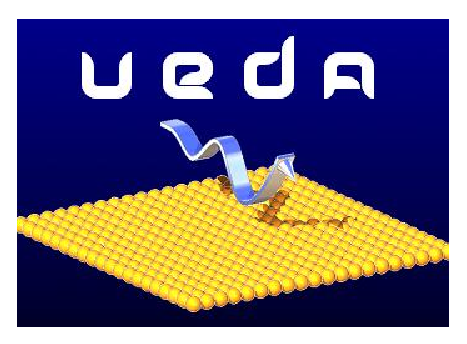
\includegraphics[width=2in]{logo2} 
\end{figure}

Copyright 2009-2020 John Melcher, Daniel Kiracofe, Shuiqing Hu, Steven
Johnson, Arvind Raman

\newpage{}

\tableofcontents{}

\newpage{}

\section{\label{sec:WhyVEDA} Why VEDA?}

Since its debut in 1986, atomic force microscopy (AFM) invented by
Rohher, Binnig et al.~\cite{Binnig_1986} has emerged as a powerful
tool in nanotechnology. In particular, dynamic atomic force microscopy
(dAFM) \cite{Martin_1987,Albrecht_1991} has proven to be an invaluable
tool that has enabled the imaging, measurement and manipulation of
matter at the molecular and atomic scale. As the ability for AFM to
measure and manipulate properties at the nanoscale has increased,
so too has the importance of understanding the tip dynamics as the
oscillating AFM probe interacts with nonlinear tip-sample interaction
forces~\cite{Garcia_SSR_2002,Garcia_PRB_1999,Hu_PRL_2006,Lee_PRB_2002,Rutzel_PROC_2003,Garcia_PRB_2000,Anczykowski_PRB_1996,Haugstad_ULTRA_1999}.
Thus the topographic images generated in dAFM scans are actually a
cumulative result of nonlinear interaction forces between the probe
tip and the sample \cite{Garcia_SSR_2002,Garcia_PRB_1999,Hu_PRL_2006,Lee_PRB_2002,Rutzel_PROC_2003,Garcia_PRB_2000,Anczykowski_PRB_1996,Haugstad_ULTRA_1999},
cantilever probe mechanics \cite{Rutzel_PROC_2003,Salapaka_JAP_1997,Stark_APL_1999,Minne_APL_1996},
tip-sample geometry convolution \cite{Montelius_APL_1993,Ramirez-Aguilar_LANG_1998,Velegol_LANG_2003,Villarrubia_1997},
and the AFM feedback control system \cite{Ashhab_AUTO_1999,Schitter_RSI_2001,El-Rifai_CEP_2007}.
Ultimately the limits of dAFM nanometrology depend on the ability
to correctly ``deconvolve'' or eliminate such spurious effects in
some manner. From an experimentalist's point of view, operating an
dAFM can often be quite non-intuitive due to the underlying nonlinear
dynamics. As a result the choice of operating conditions and cantilevers
for a specific experiment can involve much trial and error. Where
intuition fails, simulations can provide powerful insights into the
fundamental physics of this instrument. With the aid of simulation
tools like VEDA (Virtual Environment for Dynamic AFM), students and
researchers can develop a deeper quantitative understanding of dAFM.

This document attempts to provide the user with the necessary information
about the theory, modeling, and computational approach that are present
in the VEDA simulation tools, and the inputs required to perform simulations.
Additionally, several demonstration examples are provided that point
out some of the nonlinear phenomena that underpin the operation of
dynamic AFM. User are encouraged to use these examples as a starting
point to explore the vast parameter space and variety of nonlinear
phenomena present in dAFM.

VEDA \cite{Melcher_RSI_2008,kiracofe2012veda} currently includes
many different tools. Each tools corresponds to a different type of
AFM experiment. This includes 
\begin{description}
\item [{The F-Z Curves tool}] (FZC) uses the equations and solution procedure
developed for the other Approach Curves tools to simulate an the mechanics
of an undriven microcantilever approaching or retracting from a sample.
This tool is useful for observing bi-stabilities in equilibria and
the related ``snap-in'' and ``pull-off'' phenomena.
\item [{The Frequency Sweep tool}] (FS) simulates the nonlinear response
of a driven cantilever swept across resonance. Simulations of single
or multiple eigenmodes are possible.
\item [{Dynamic Approach Curves}] simulates an AFM cantilever excited
near resonance and brought towards a sample surface. Several different
versions are available: Amplitude modulation (i.e. tapping mode) and
Frequency modulation. The AM tool has both a basic and advanced version.
The basic tool is suitable for simulating either ambient conditions
or ultra high vacuum (UHV). The advanced tool is an expanded version
of the basic tool allowing both multiple eigenmode simulations as
well as multiple excitation frequencies. This tool is designed specifically
for simulating approach/retraction curves in liquids, bimodal excitations,
and internal resonance (harmonic cantilevers) applications. The model
for cantilever dynamics includes a general number of eigenmodes and
users are able to specify either acoustic (base) and magnetic excitation
sources with single or multiple frequencies. The frequency modulated
version simulates the situation where the AFM cantilever is excited
at a frequency that is tuned to the nonlinear natural frequency through
the use of a phase locked loop (PLL) and amplitude is maintained constant
with an active feedback loop.
\item [{Scanning tools}] simulates scans over specified geometric features
with heterogeneous material properties. Several different version
are available corresponding to contact mode, amplitude modulated (i.e.
tapping mode), and frequency modulation. Both basic and advanced versions
of the Amplitude Modulated tool are also available, corresponding
to the same feature sets as the basic and advanced Amplitude Modulated
Approach Curves tools, respectively.
\end{description}
\newpage{}

\section{\label{sec:intro}Basic concepts and terminology}

In this section we will introduce basic AFM concepts and terminology
for the benefit of beginning AFM users. Additionally, schematics are
provided to illustrate relevant coordinates and reference frames.

\subsection{Basic AFM design}

A schematic of the standard AFM is shown in Figure \ref{fig:schematic}.
A microcantilever probe with a sharp tip (Figure \ref{fig:cant_sem})
interacts with a sample. The position of the sample is controlled
by a stage with piezo actuators. To create an image, the sample is
moved so that the microcantilever probe tip rasters over the sample.
The precise method by which an image of the sample's surface is generated
from the raster depends on the imaging mode. However, in general,
creating an image of the surface topography in AFM involves monitoring
some characteristic measure (deflection, amplitude, phase, etc.) of
the cantilever deflection caused by the interactions forces between
the tip and the sample. Measurements of the microcantilever deflection
have been made in a variety of ways. In the most common method, the
optical-lever technique, a laser beam is reflected off of the cantilever
and detected by a quadrature photodetector. For small deflections
of the probe, signal of the photodetector is proportional to the change
in slope (angle) of the microcantilever.

\begin{figure}[h]
\includegraphics[width=0.4\textwidth]{schematic} 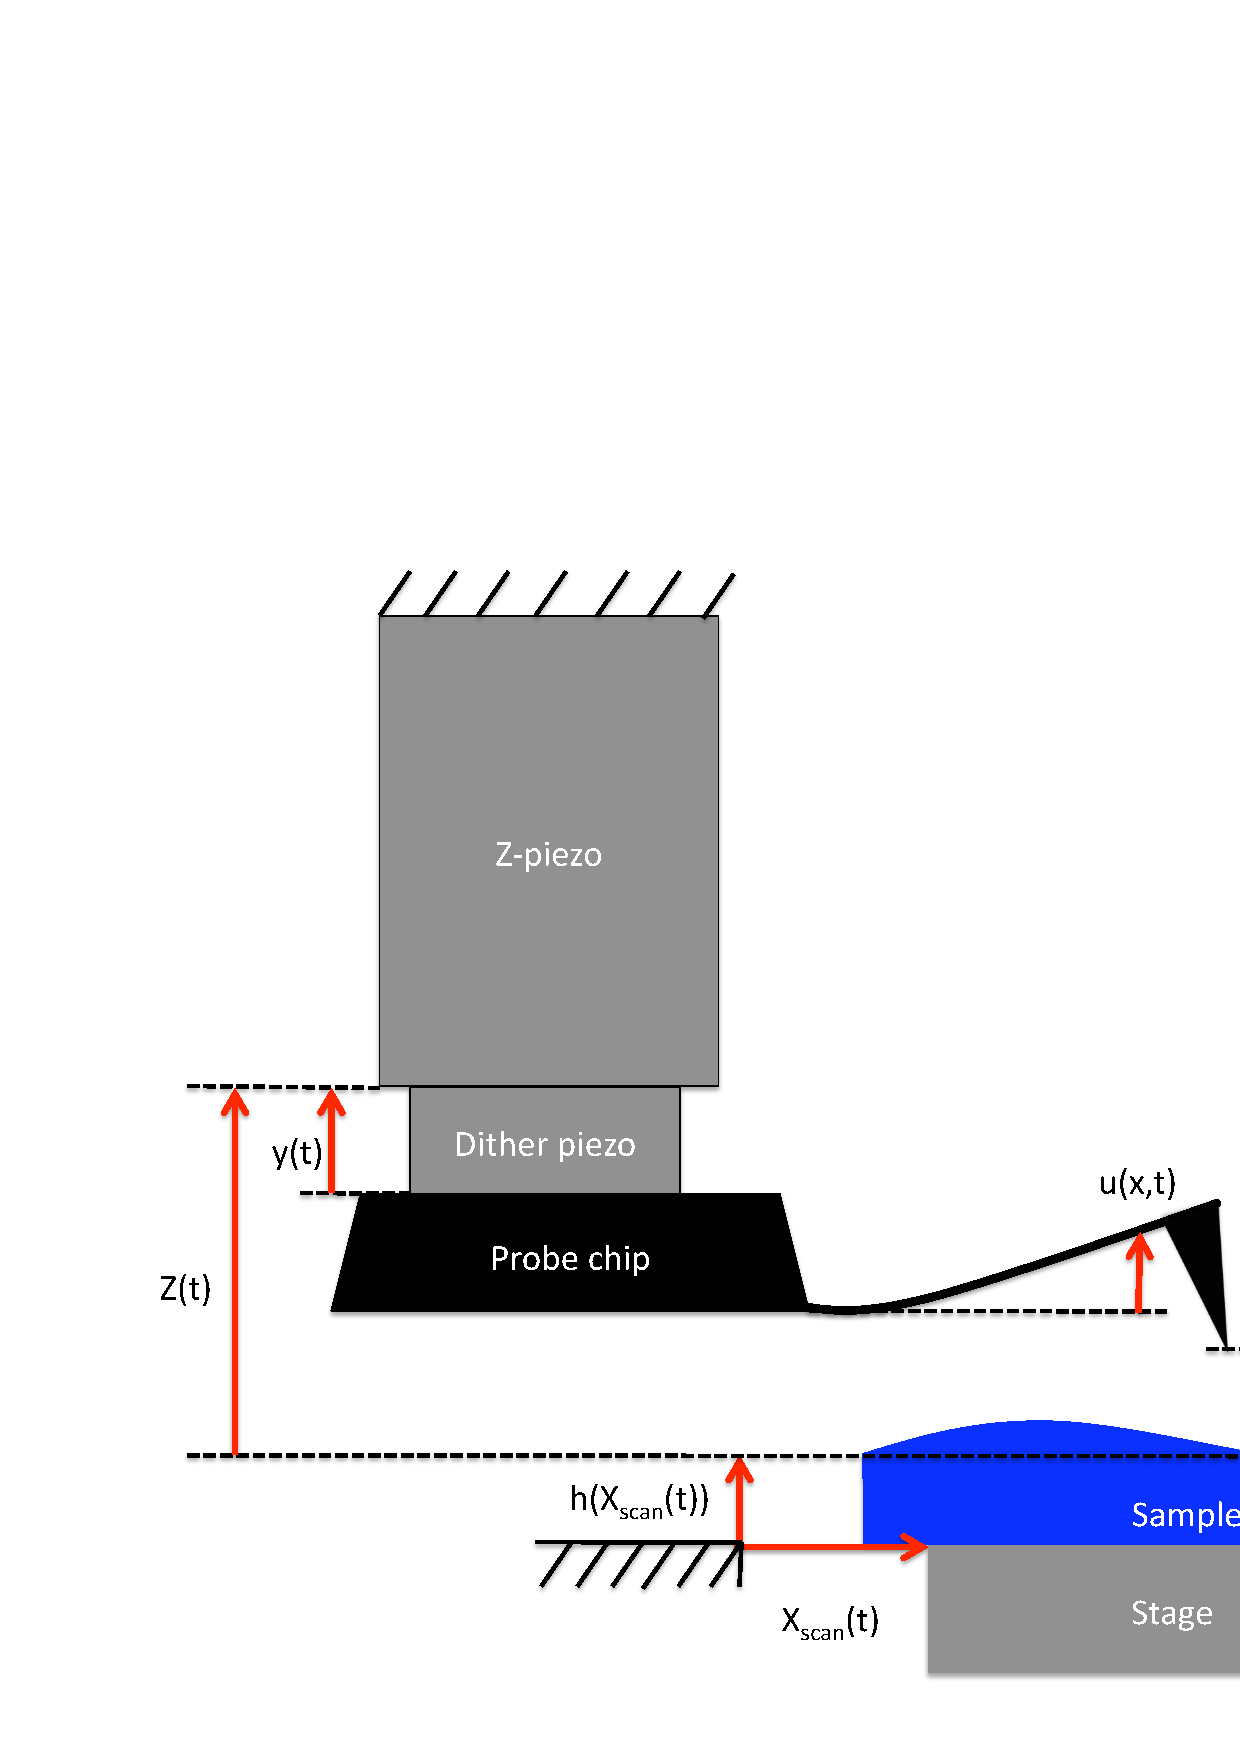
\includegraphics[width=0.6\textwidth]{coords_schematic}
\caption{A schematic of basic AFM operation (top \cite{Hu_thesis}) and important
coordinates (bottom). The Z-piezo expands or contracts in order to
modify the Z distance $Z(t)$. The dither piezo is used to excite
the cantilever by shaking the base (acoustic excitation) by $y(t)$.
The transverse deflection relative to the base is $u(x,t)$, where
$x$ is the axial displacement from the base. Scanning is achieved
by varying $X_{scan}(t)$ by a constant scanning velocity $V_{scan}=X_{scan}(t)/dt$.
The instantaneous gap between the tip and the sample is $d(t)=Z(t)+y(t)+u(L,t)$,
where the Z distance $Z(t)$ is modified by the Z-piezo extension/displacement
or variations in the sample height $h(t)$.}

\label{fig:schematic} 
\end{figure}

\begin{figure}[h]
\includegraphics[width=0.4\textwidth]{NSC12_small} \caption{SEM image of a typical AFM cantilever. The imaging tip is in the lower
right.}

\label{fig:cant_sem} 
\end{figure}

Components of the AFM along with relevant coordinates are shown in
Figure \ref{fig:schematic}. Simulations approaching the sample, either
statically (F-Z curves) or with an oscillating probe are achieved
through extensions of the Z-piezo to reduce the Z distance $Z(t)$.
While the cantilever is approaching the sample, the stage is fixed
($X_{scan}$ is constant). While cantilever is scanning over the sample,
the stage moves the sample at a constant rate $X_{scan}(t)$ at a
constant rate $V_{scan}=dX_{scan}(t)/dt$.

\subsection{Imaging modes}

There are myriad different AFM operating modes, all of which are built
on the basic design above. These different modes have different strengths
and weaknesses, and a particular task may be better served by one
mode than another. A taxonomy of the major AFM modes is shown in Figure
\ref{fig:imaging_modes}. There is a major division between static
modes and dynamic modes. In dynamic modes, the cantilever probe is
excited (typically at resonance) as it is scanned over the surface.
In static modes, the probe is not excited. Within static modes, two
of the major modes are contact mode and force-volume mode. In contact
mode, the probe is essentially in contact with the sample at all times.
In force-volume mode and the related jump mode, the probe touches
a point, retracts, moves to the next point, approaches, and touches
the next point. Both of these modes are built upon force-distance
curves, also known as F-Z Curves. In dynamic modes, two of the main
modes are amplitude modulated (AM) and frequency modulated (FM). These
names can be confusing because in both AM and FM modes a feedback
controller is used to keep the vibration amplitude constant during
a scan. In AM mode, the height of the probe above the sample is what
is used to keep the vibration amplitude constant, while in FM mode,
a more complicated feedback scheme is used that attempts to keep the
oscillation amplitude, phase, and frequency shift constant while scanning
the sample.. These feedback schemes are described in more detail in
Section \ref{sec:theory}.

\begin{figure}[htb]
\includegraphics[clip,width=0.5\textwidth]{imaging_modes} \caption{A taxonomy of some major AFM modes.}

\label{fig:imaging_modes} 
\end{figure}

A diagram of the operation of contact mode, AM, and FM modes is shown
in Figure \ref{fig:scanning}. Note that FM-AFM (Figure \ref{fig:scanning}b)
is shown scanning far away from the sample to indicate operation in
the attractive regime, and that AM-AFM (Figure \ref{fig:scanning}c)
is shown closer to the sample to indicate intermittent contact or
repulsive regime. Although this is usually the way the two modes are
used in practice, it is not the distinguishing characteristic. AM-AFM
can be used in the attractive regime and FM-AFM can be used in the
repulsive regime. The distinguishing characteristic between the two
modes is the feedback scheme.

VEDA was originally written with AM-AFM in mind. Later expansions
have allowed simulations of F-Z/F-d Curves and FM methods.

\begin{figure}[htb]
\includegraphics[width=0.5\textwidth]{scanning} \caption{Schematic diagrams of the operation mechanisms for (a) contact mode
AFM, (b) FM-AFM, and (c) AM-AFM. Taken from \cite{Hu_thesis}}

\label{fig:scanning} 
\end{figure}

%Arvind's comment on this figure:  I would (a) label quantities in red that are kept constant with feedback i.e. in AM-AFM only the A and in FM-AFM it should be A, , phi and delta f - these are the feedback variables (b) label the control variables in say blue...i.e. in contact mode Z(t) and also in AM-AFM, but in FM-AFM you should have Z(t), f(t), and y(t)....



\subsection{Excitation methods}


With dynamic modes, there are many different methods by which the
cantilever can be vibrated. Two of the most common are acoustic mode
and magnetic mode. Figure \ref{fig:mag-v-aco} shows these two methods
schematically. In the magnetic mode, a magnetic coating (or magnetic
particles) is applied to the cantilever and a solenoid provides an
alternating magnetic field that drives the cantilever. In acoustic
mode, a so-called dither piezo vibrates up and down. which moves the
base of the cantilever up and down. Note that due to the readout scheme
used in most AFMs, the absolute deflection of the cantilever cannot
be accessed but only the deflection relative to the base (bending).
This can cause significant complications for acoustic mode in low
Q (e.g. liquid) operation. More details on the difference between
these excitations can be found in \cite{Xu_JAP_2007}

\begin{figure}[htb]
\includegraphics[width=0.7\textwidth]{acoustic_vs_magnetic} \caption{A schematic showing the different tip motions measured in the magnetic
mode and acoustic mode. In magnetic mode the measured tip motion is
the absolute tip motion $w(x,t)$. While in the acoustic mode the
measured motion $w(x,t)$ (transverse cantilever deflection) is the
motion $u(x,t)$ relative to the base motion $y(t)$. Reproduced from
\cite{Xu_JAP_2007}}

\label{fig:mag-v-aco} 
\end{figure}



\subsection{Photodiode output}


In this section, we demonstrate why the photodiode is more sensitive
to slope than displacement.

In \ref{fig:photodiode}, we see that if a flat mirror is moved down,
the laser spot will move on the photodiode. Similarly, if a flat mirror
is rotated, the laser spot will move on the photodiode. Now for a
cantilever, there will be some displacement at the end and some slope.
There will be contributions from both. But which is more sensitive?

The static bending shape of a cantilever is given by $g(x)=1-0.5{(x/L)}^{2}(3(x/L))$,
where $L$ is cantilever length. This means that the slope $g^{\prime}(L)=-1.5/L$.
In other words, for a bending displacement of $h$, the cantilever
has a slope at the end of $1.5h/L$, which means the rotation angle
is $d\theta=\arcsin(1.5h/L)$. Because the angles are small, $\sin(d\theta)\approx d\theta$.
So, for bending displacement of $h$, the laser spot moves $H*2*1.5h/L$.

For example assume H = 1 cm, $\theta$=45 deg, h=1e-9, L=100e-6 Then
the displacement contribution to spot movement is 1.4e-9 = 1.4 nm
and the rotation contribution is H{*}2{*}1.5h/L = 2e-7 = 200 nm. In
other words, the displacement contribution is less than 1 percent
of the rotation contribution. For this reason, we typically ignore
the displacement contribution.

\begin{figure}[htb]
\includegraphics[width=0.7\textwidth]{photodiode} \caption{A schematic explaining why the photodiode measures slope and not true
deflection}

\label{fig:photodiode} 
\end{figure}

\newpage{}




\section{\label{sec:Tools}Tools}

\subsection{\label{sec:Tools.DAC}Amplitude Modulated Approach Curves (AMAC,
basic)}

At the backbone of dAFM is the assumption that the microcantilever's
oscillations are affected by nonlinear interactions between the tip
and sample. In particular, in AM-AFM, the amplitude of the microcantilever
is affected by of both attractive and repulsive forces interactions
between the tip and the sample. This occurs primarily because of the
detuning on the nonlinear natural frequency from the fixed excitation
frequency as the probe approaches the sample. However when the oscillation
amplitude is much smaller than the decay length of the interaction
forces, there is also a shift in linear frequency of the oscillator
which can reduce the driven oscillation amplitude. Monitoring characteristics
of the microcantilever's oscillation while approaching a sample reveals
information about the mechanical properties of the sample and of tip-sample
interaction (imaging) forces. Additionally, an appropriate set-point
amplitude for use in AM-AFM scanning (and simulated by the AMS tool)
can be determined. The Amplitude Modulated Approach Curves (AMAC)
tool can be utilized to simulate the response of a microcantilever
excited near it's fundamental resonance and gradually introduced to
the sample by extending the Z-piezo and reducing the $Z$ distance
between the base and the sample. Input parameters for AMAC (basic)
include the properties of the cantilever and the tip-sample interactions,
as well as operating conditions and simulation parameters.

The following assumptions have been made in the AMAC tool (in addition
to the assumptions made in the models): 
\begin{enumerate}
\item Cantilever dynamics are modeled by a single eigenmode model (Eq. \ref{eq:ndmdof}
for $i=1$). 
\item Interactions between the tip and the sample are modeled by any one
of the models given in Sec. \ref{sec:fts}. 
\item The cantilever is either acoustically or magnetically excited with
a single frequency. 
\item The $Z$ distance between the sample can be reduced or increased,
but the cantilever does not move laterally. Inertial and hydrodynamic
forces caused by the $Z$ motion are negligible. 
\end{enumerate}
This section provides an overview of the outputs of the Amplitude
Modulated Approach Curves (AMAC) tool in the form of three example
simulations.

\begin{table}[H]
\caption{\label{tab:DACEx}Input parameters for AMAC examples.}

\begin{ruledtabular} %
\begin{tabular}{lrrr}
~~~~\textbf{PARAMETER} & \textbf{EXAMPLE 1} & \textbf{EXAMPLE 2} & \textbf{EXAMPLE 3}\tabularnewline
~ &  &  & \tabularnewline
\textbf{Operating conditions and cantilever properties} &  &  & \tabularnewline
~~~~Unconstrained amplitude (nm) & 30 & 30 & 60\tabularnewline
~~~~$k$ (N/m) & 40 & 40 & 3\tabularnewline
~~~~$Q$ & 400 & 400 & 150\tabularnewline
~~~~$f$ (kHz) & 350 & 350 & 75\tabularnewline
~~~~$f_{d}$ (kHz) & 350 & 350 & 75\tabularnewline
~~~~Z approach velocity (nm/s) & 200 & 200 & 200\tabularnewline
~~~~Z range Determination & Autocalc & Specify & Autocalc\tabularnewline
~~~~Initial Z separation (nm) & NA & 0 & NA\tabularnewline
~~~~Final Z separation (nm) & NA & 35 & NA\tabularnewline
~ &  &  & \tabularnewline
\textbf{Tip-sample interaction properties} &  &  & \tabularnewline
~~~~Tip-sample interaction model & DMT contact & DMT contact & Hertz contact\tabularnewline
~~~~Tip radius (nm) & 20 & 20 & 10\tabularnewline
~~~~Young's modulus of tip (GPa) & 130 & 130 & 130\tabularnewline
~~~~Poisson's ratio of the tip & 0.3 & 0.3 & 0.3\tabularnewline
~~~~Auto calculate intermolecular distance? & no & no & n/a\tabularnewline
~~~~Intermolecular distance (nm) & 0.164 & 0.164 & n/a\tabularnewline
~~~~Hamaker constant (J) & $7.1\cdot10^{-20}$ & $7.1\cdot10^{-20}$ & n/a\tabularnewline
~~~~Young's modulus of sample (GPa) & 1.2 & 1.2 & 1\tabularnewline
~~~~Poisson's ratio of the sample & 0.3 & 0.3 & 0.3\tabularnewline
~~~~Sample visco-elastic forces? & none & none & Kelvin-voigt\tabularnewline
~~~~Sample viscosity ($Pa\cdot s$) & NA & NA & 500\tabularnewline
~ &  &  & \tabularnewline
\textbf{Simulation parameters} &  &  & \tabularnewline
~~~~Number of points plotted & 500 & 500 & 500\tabularnewline
~~~~Deflection points per cycle & 400 & 1000 & 1000\tabularnewline
~~~~Include time histories & yes & no & yes\tabularnewline
~~~~Number of time histories & 1 & NA & 1\tabularnewline
~~~~Choose amplitude ratio(s) & 0.55 & NA & 0.55\tabularnewline
~~~~Number of cycles & 5 & NA & 5\tabularnewline
~~~~Choose X-axis variable & Z-distance (nm) & Z-distance (nm) & Z-distance (nm)\tabularnewline
\end{tabular}\end{ruledtabular} 
\end{table}

\newpage{}



\subsubsection{\label{sec:Tools.DAC.Ex1}Example 1: Attractive and repulsive regimes
of oscillation}


In this example, two different regimes of oscillation are explored.
The attractive regime refers to oscillations where the interaction
forces between the tip and sample are primarily attractive. Likewise,
the repulsive regime refers to oscillations where the interactions
with the sample are primarily repulsive contact forces. Proper identification
of the attractive and repulse regimes is critical for an AFM experimentalist
for improving imaging resolution, avoiding imaging bi-stabilities
and correctly interpreting of phase contrast images. This first example
is aimed at reproducing some of the key results from Garcia and San
Paulo \cite{Garcia_PRB_1999}.

After opening VEDA, select \textit{Amplitude Modulated Approach Curves
(basic)} from the pull-down menu labeled {\em Application}. Once
the interface for the AMAC tool is loaded, there is a second pull-down
menu titled {\em Example loader}. Select {\em Example 1: Attractive
and repulsive regimes of oscillation} and the inputs for this example
listed in Table \ref{tab:DACEx} will be loaded automatically into
the interface. Take a moment to peruse the three input panels.

The first tab is {\em Operating conditions and cantilever properties}
and it contains the following input parameters: 
\begin{description}
\item [{Unconstrained amplitude}] this is the amplitude when the cantilever
is very far from the sample, sometimes called free amplitude or initial
amplitude. 
\item [{k (N/m)}] represents the cantilever stiffness of the fundamental
eigenmode. 
\item [{Q}] represents the quality factor of the resonance. The quality
factor is a measure of the sharpness of the resonance peak and is
easily determined experimentally from a frequency sweep or ``tuning
curve''.
\item [{ Nat. Freq (kHz)}] represents the fundamental natural frequency
in kilohertz. 
\item [{ Driving Freq. (kHz)}] represents the drive frequency, or excitation
frequency applied by the excitation source (acoustic or magnetic)
to the microcantilever. 
\item [{Z approach speed (nm/s)}] represents the average speed of the
Z piezo (i.e. the speed at which the base of the microcantilever approaches
the sample) in nanometers per second. 
\item [{Z range determination}] allows a few different options to specificy
the initial and final Z displacements of the base of the microcantilever.
For the purposes of this example, the autocalculated values will be
fine (in this case it will 5 nm above where the tip contacts the sample,
which is Z=35 nm because the unconstrained amplitude is 30 nm) 
\end{description}
The second tab is {\em Tip-sample interaction properties}. There
are several input parameters on this tab; however, the user required
only to input parameters relevant to the choice of tip-sample interaction
model. In this example, we choose the {DMT contact} model, which
is selected from the pull-down menu at the top of this panel. The
DMT contact model requires the following inputs:
\begin{description}
\item [{Tip radius (nm)}] represents the radius of the cantilever tip,
in nanometers, which will come into contact with the sample. 
\item [{Young's modulus of tip (GPa)}] represents the stiffness of the
elastic tip material. More precisely, the Young/s modulus is a relationship
between stress and strain for an elastic element according to Hooke's
law. For silicon (Si), $E\approx130$ GPa. 
\item [{Poisson's ratio of the tip}] represents the Poisson's ratio of
the material used in the cantilever's tip. This parameter is used
in all tip-sample interaction models except for the two linear-contact
models. The Poisson's ratio is a material property that relates a
uniaxial strain induced in a specific direction due to a stress applied
in the orthogonal direction. 
\item [{Auto calculate intermolecular distance}] gives the user the opportunity
to have the intermolecular distance $a_{0}$ automatically calculated.
If the box is checked (``yes''), $a_{0}$ will be calculated for
the DMT and DMT+DVLO models using the van der Waals adhesion force,
the tip radius, and the Hamaker constant. If unchecked (``no''),
the van der Waals adhesion force will be calculated from $a_{0}$,
the tip radius, and the Hamaker constant. This option is provided
solely for convenience. In either case, the component of the adhesion
resulting from the van der Waals forces is $F_{ad,vdW}=HR/6a_{0}^{2}$
(see tip-sample interaction models in the theory in Section \ref{sec:fts}). 
\item [{van der Waals adhesion force (nN)}] represents the component of
adhesion force, measured in nanonewtons, attributable to attractive
van der Waals forces. If the DMT contact model is applicable, the
adhesion forces is the ``pull-off'' force that can be found experimentally
from a static force-distance curve 
\begin{equation}
F_{ad}=|k_{c}\times w^{*}|,
\end{equation}
where $k_{c}$ is the static bending stiffness of the cantilever,
and $w^{*}$ is the deflection of the tip at the ``pull-off'' location
as the cantilever is withdrawn from the surface.
\item [{Hamaker constant (J)}] represents the value used to predict the
attractive van der Waals forces between the tip and the sample. This
parameter depends on the material of both the tip and the sample,
as well as the surrounding material.
\item [{Young's modulus of the sample (GPa)}] represents the stiffness
of the sample material.
\item [{Poisson's ratio}] of the sample: see Poisson's ratio of the tip
above.
\item [{Solvation forces}] this is applicable only for liquids, and thus
is not relevant to this example.
\item [{Nonconservative forces}] Allows users to include non-conservative
interaction forces between the tip and the sample. Non-conservative
dissipate mechanical energy of the probe during interaction. This
example does not call for including such forces. 
\end{description}
The third and final tab is {\em Simulation parameters}, which contains
input parameters relating to the simulation, but not the physics of
the problem. Relevant inputs in this example are: 
\begin{description}
\item [{Number of points plotted: }] This is the number of points contained
in each plot. This values of this parameter may be increased if the
user is interested in abrupt features in the results. 
\item [{Speed versus accuracy tradeoff: }] This controls the number points
that the differential equation solver computes in each drive cycle.
Using more points will give a more accurate result, but will take
longer to compute. 
\item [{Include time histories: }] The default outputs of VEDA are quantities
such as amplitude and phase that are averaged over several drive cycles
(similar to a real AFM). This option allows the user to examine the
raw data of each individual cycle (similar to hooking up an oscilloscope
to the AFM and viewing the raw voltage traces). 
\item [{Choose X-axis variable: }] Choose whether to plot simulation data
against $Z$ distance or against amplitude ratio ($A_{1}/A_{0}$) 
\end{description}
After reviewing that the input parameters, click on the Simulate button.
The simulation results for the input parameters are available by selecting
a result from the pull-down menu once the simulation has concluded.
The following provides a brief discussion of each result.

A few minutes after pressing the simulation button, the plot in Figure
\ref{fig:DAC_Ex1_AZ} should appear. Simulations running much longer
than a few minutes are likely due to erroneous or non-physical input
parameters. If these occurs even though the inputs parameters are
correct, please submit a support ticket by selecting the Help! button.

Figure \ref{fig:DAC_Ex1_AZ} shows that, as the cantilever approaches
the sample from right to left, there is first a reduction in amplitude
due to the attractive van der Waals interaction \cite{Garcia_PRB_1999}.
This reduction is due to the attractive interaction forces detuning
the nonlinear resonance frequency of the probe tip from the fixed
excitation frequency. This detuning also causes the phase of the first
harmonic to increase above 90 degrees, as shown in Figure \ref{fig:DAC_Ex1_Phase}.
The onset of repulsive regime is marked by a jump in amplitude and
corresponding jump in phase to a value less than 90 degrees.

\begin{figure}
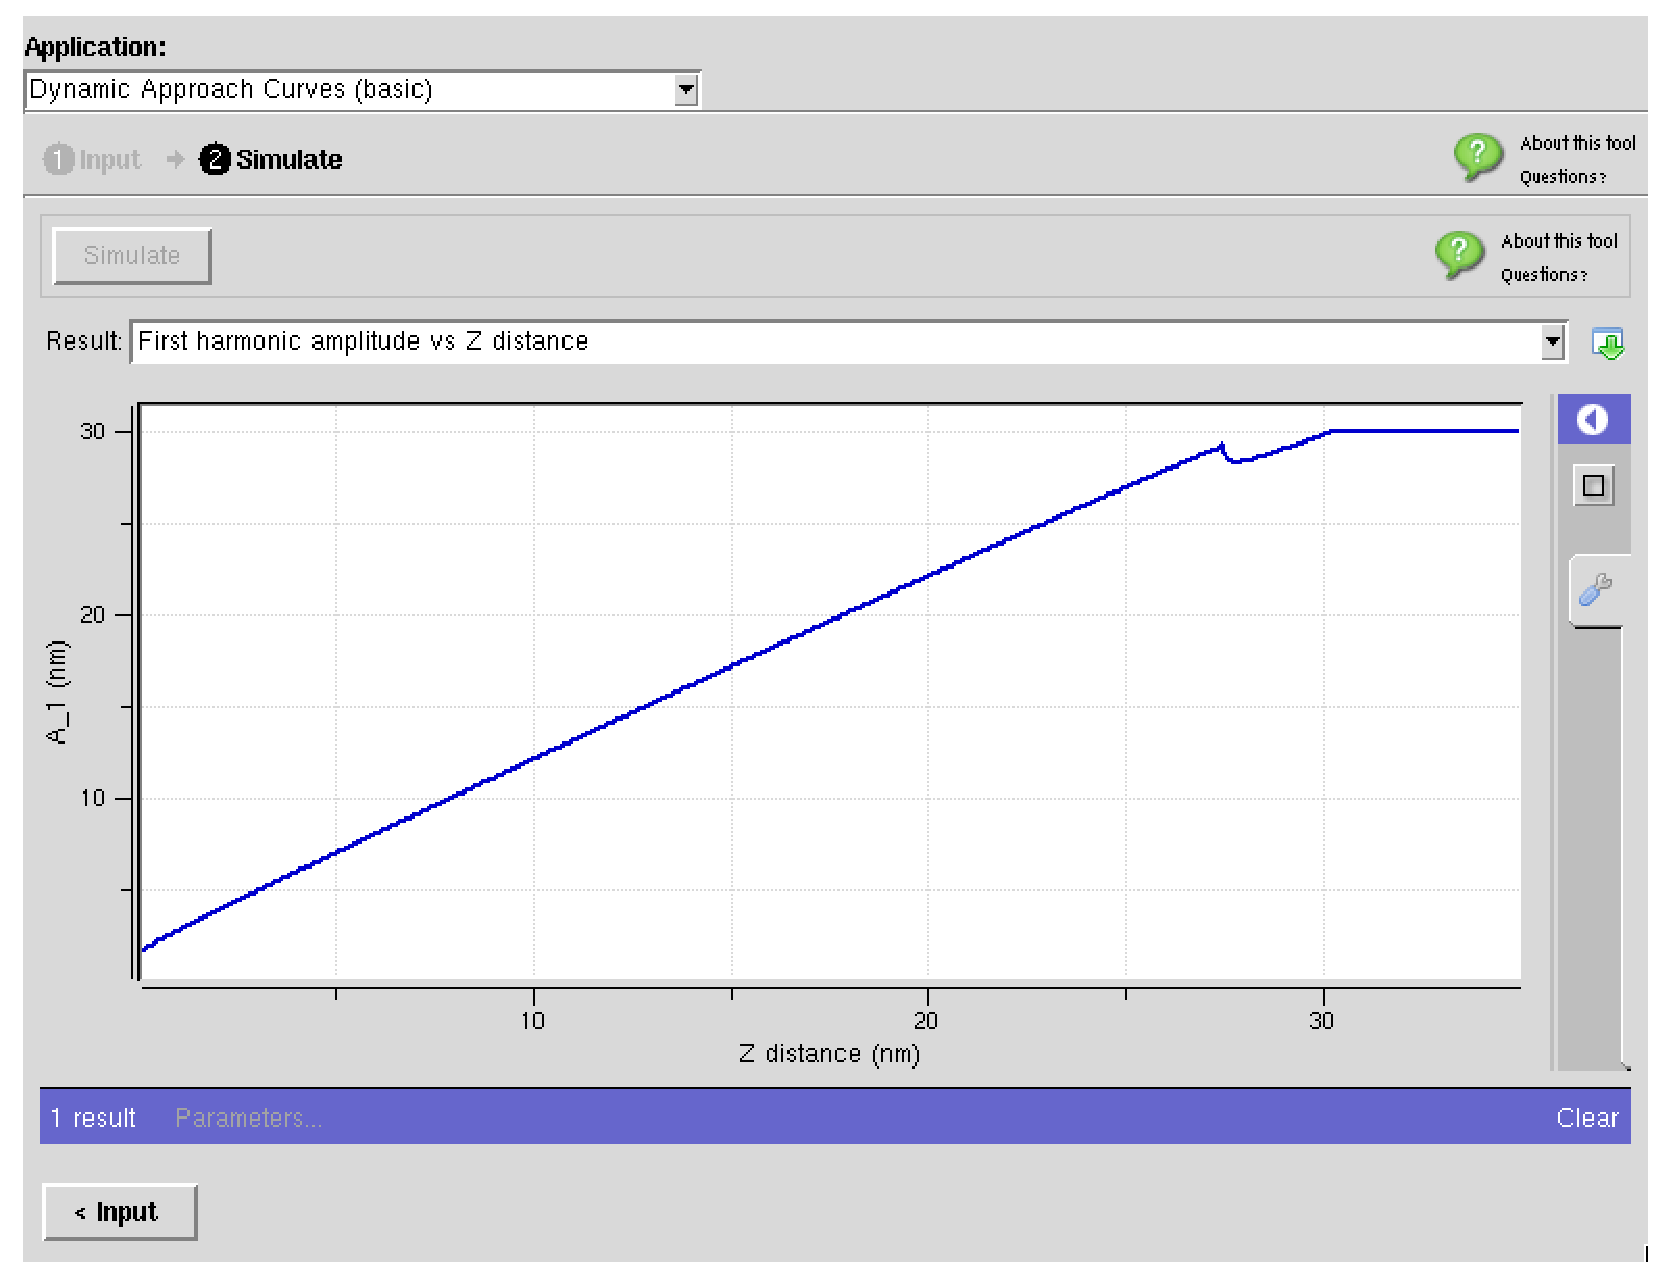
\includegraphics[width=5in]{DAC_Ex1_AZ} \caption{\label{fig:DAC_Ex1_AZ} Amplitude of the first harmonic vs. $Z$ distance
during approach to the sample. The abrupt change in amplitude marks
the transition from the attractive to the repulsive regime of oscillations.
(AMAC Ex 1)}
\end{figure}

%Arvind's comment: can you label attractive and repulsive regimes above with a dashed line?

\begin{figure}
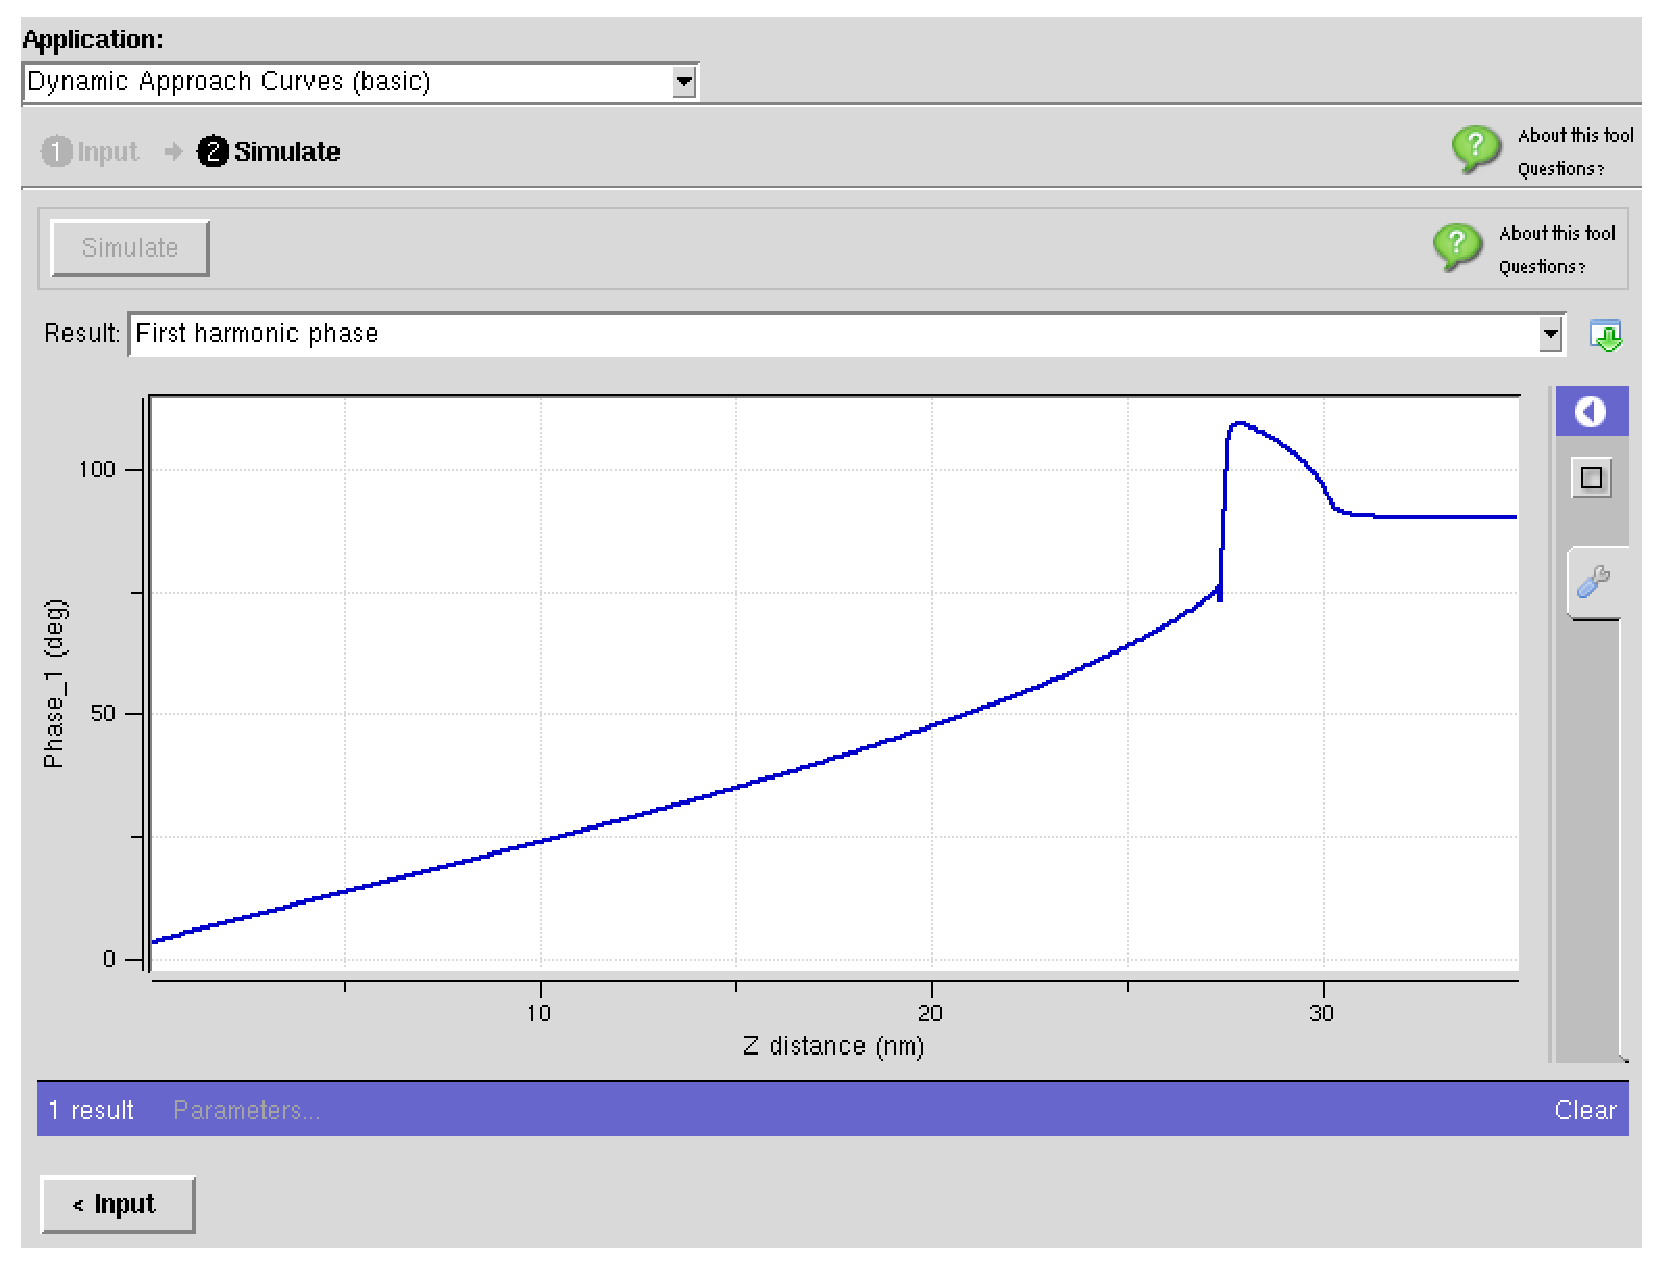
\includegraphics[width=5in]{DAC_Ex1_Phase} \caption{\label{fig:DAC_Ex1_Phase} Phase of the first harmonic vs. $Z$ distance
during approach to the sample. A phase greater than 90 degrees indicates
the attractive regime while a phase of less than 90 indicates the
repulsive regime. (AMAC Ex 1)}
\end{figure}

While approaching the sample, the first harmonic phase first increases
about 90 degrees in the attractive regime of oscillations due to the
softening of the nonlinear natural frequency. At this point, the nonlinear
natural frequency has been detuned (decreased in this case) from the
fixed excitation frequency applied to the probe. This results in a
phase greater than 90 degrees. Continuing to approach the sample,
a jump from the attractive to the repulsive regime occurs at a $Z$
distance around 27 nm. This jump is marked by a phase less than 90
degrees in Figure \ref{fig:DAC_Ex1_Phase}. In the repulsive regime,
the nonlinear natural frequency stiffens, and is now greater than
the fixed excitation frequency applied to the probe. If the user repeats
the simulations for an excitation frequency $f_{d}$ not equal to
the natural frequency $f$ (say 200 Hz above or below) the results
will be slightly different because the detuning effects of the attractive
and repulsive regimes will accomplish different results.

\begin{figure}[htp]
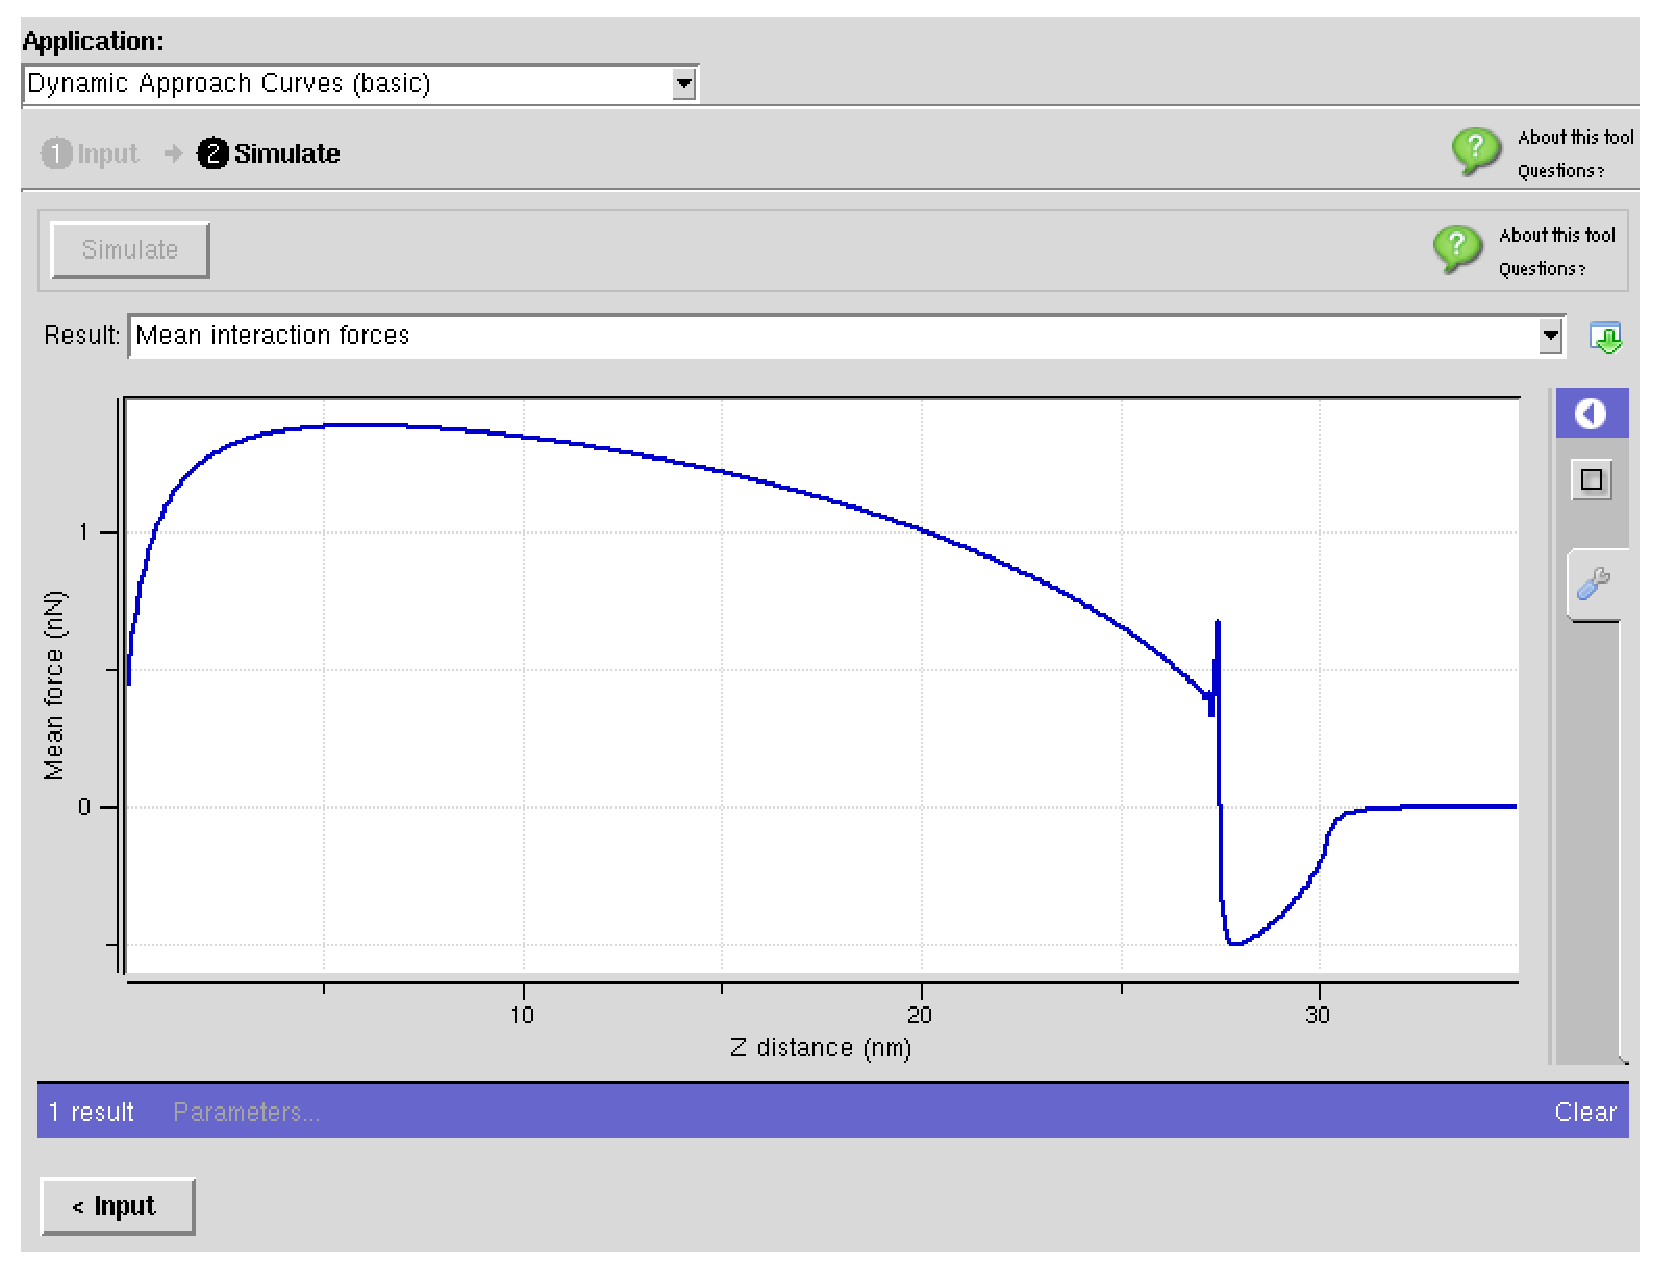
\includegraphics[width=5in]{DAC_Ex1_MF} \caption{\label{fig:DAC_Ex1_MF} Mean (oscillation cycle averaged) tip-sample
interaction forces during approach. Mean forces are negative in the
attractive regime and positive in the repulsive regime. (AMAC Ex 1)}
\end{figure}

As the cantilever proceeds through the attractive regime, there is
eventually a sharp change in amplitude as the probes transitions from
the attractive to the repulsive regime. By comparing the mean forces
(Figure \ref{fig:DAC_Ex1_MF}) to the amplitude (Figure \ref{fig:DAC_Ex1_AZ})
and phase (Figure \ref{fig:DAC_Ex1_Phase}), the user will find that
the jumps in amplitude and phase occur precisely when the mean forces
change abruptly from negative (attractive) to positive (repulsive).
In this example, the change occurs around Z = 27 nm. Hence, the two
regimes have been dubbed the attractive regime and the repulsive regime
according to the mean interaction force observed during oscillation.

Figure \ref{fig:DAC_Ex1_Def} contains a sample of photodiode deflection
signal $u_{p}(t)$ and interaction force histories containing five
complete cycles. The histories shown in Figure \ref{fig:DAC_Ex1_Def}
correspond to 1000 points per cycle. This number is likely to be sufficient
for most simulations. To accurately record very small time-scale interactions,
however, the user may wish to increase the value of the parameter.
It is important to note that the tip-sample interactions are not directly
measured in dAFM.

\begin{figure}
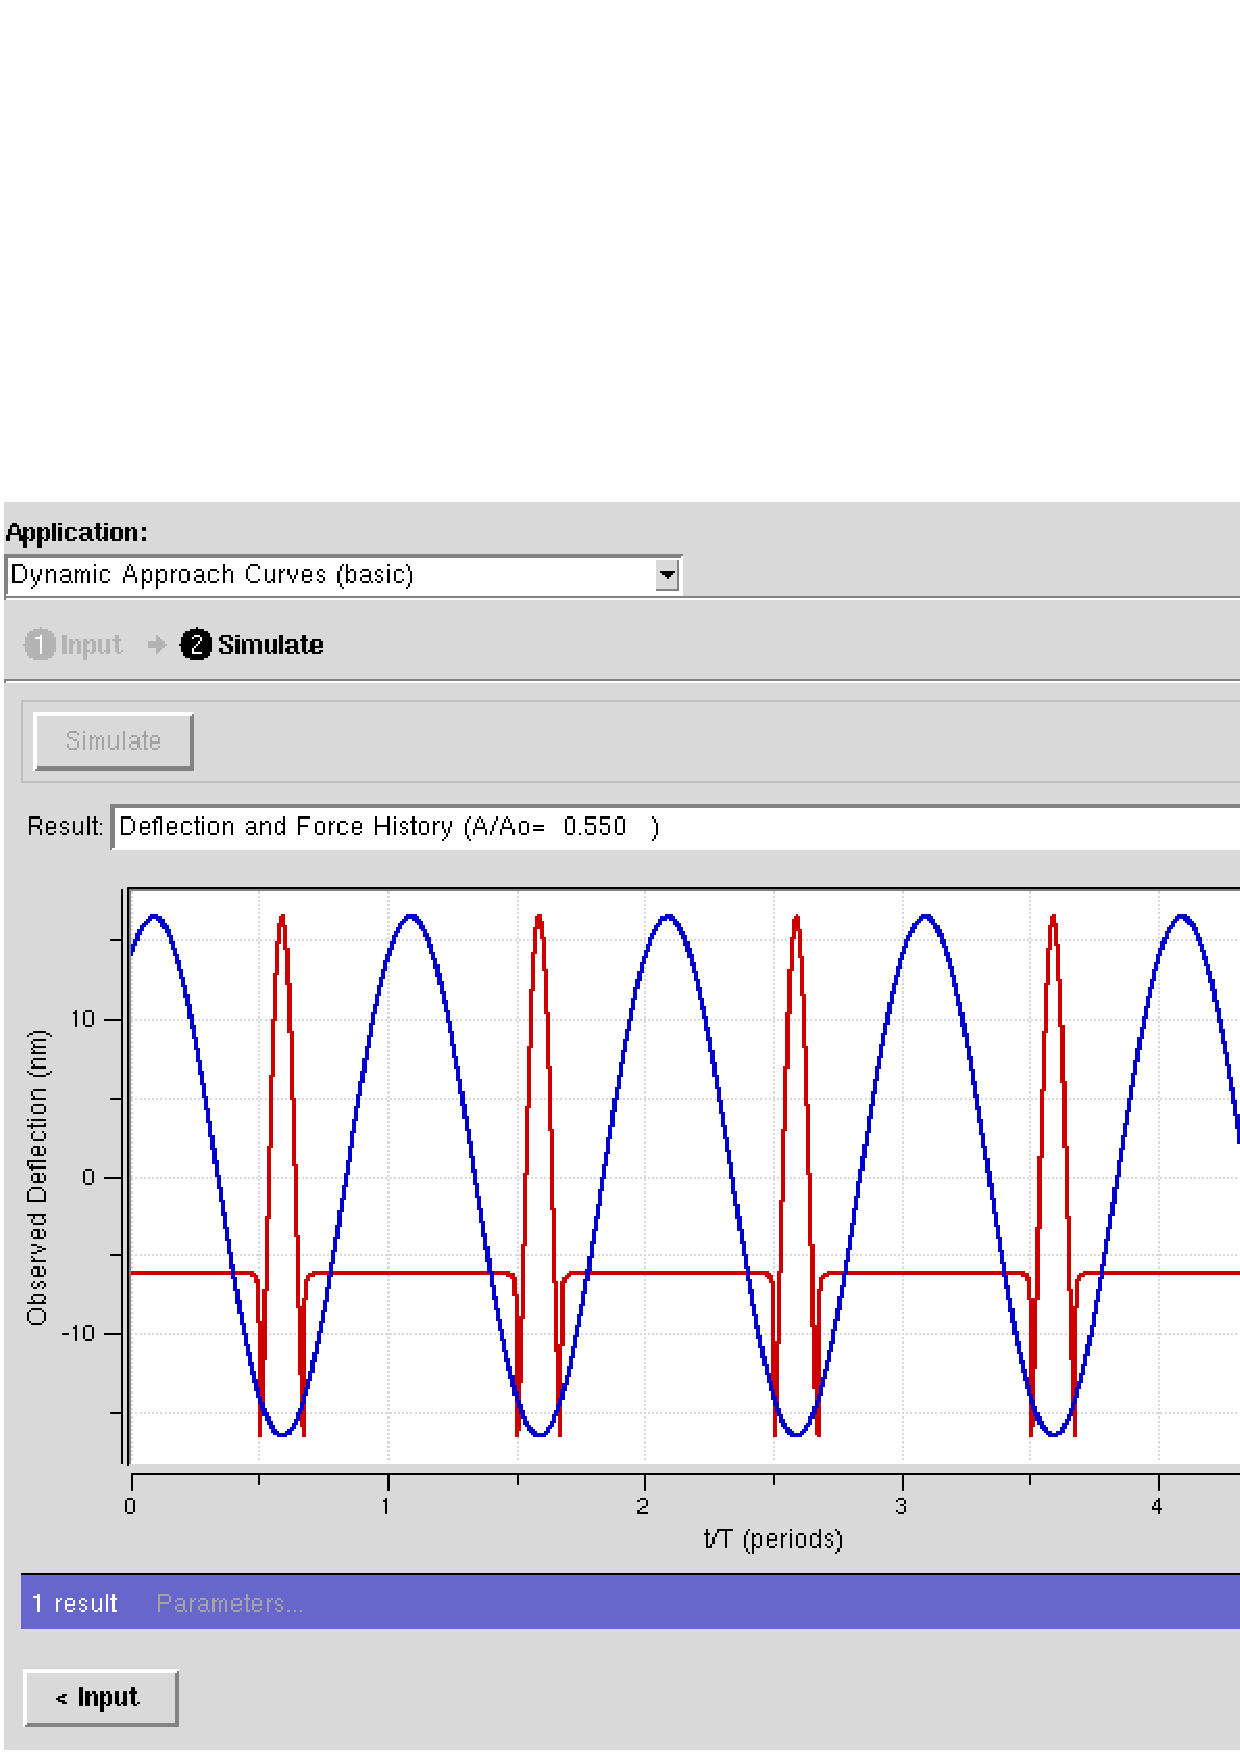
\includegraphics[width=5in]{DAC_Ex1_Def} \caption{\label{fig:DAC_Ex1_Def} Deflection signal from the photodiode accompanied
by the corresponding tip-sample interaction force (setpoint = 0.55
\%). (AMAC Ex 1) }
\end{figure}



\subsubsection{\label{sec:Tools.DAC.Ex2}Example 2: Retraction curves}


In this example, we investigate the tip dynamics during cantilever
retraction from the surface. The cantilever/sample parameters used
are the same in AMAC Example 1 (Section \ref{sec:Tools.DAC.Ex1}).
Retraction curves are particularly interesting when the approach curves
show a discontinuous amplitude jump from attractive to repulsive regimes
of oscillation. In fact it can be shown \cite{Garcia_PRB_1999} that
there is a noticeable amplitude hysteresis between approach and retraction
curves.

We recommend completing AMAC Example 1 before proceeding to this example
so the user can will be able to study the hysteresis due to the bi-stable
oscillation regimes. The physical parameters, such as the cantilever
properties and tip-sample interaction parameters, of this simulation
are identical to the first example; however, we have changed the operating
and simulation parameters to simulate retraction from the sample.
The retraction is achieved by changing \emph{Z range determination}
to {\em Specify Z range} and change the initial Z separation to
0 nm and the final Z distance to 35 nm. The default Z range for the
simulation is from 5 nm greater than the unconstrained amplitude (30
nm) to 0 nm. For this simulation we have simply inverted the default
Z range.

If you have not already run AMAC Example 1, then follow these instructions:
open the \textbf{AMAC} (basic) tool from the \textbf{VEDA} tools selection.
Wait for the user input window to open. Under the \emph{Operating
conditions and cantilever properties} tab, set the \emph{Unconstrained
amplitude (nm)} to 30, and set \emph{$k_{i}$ (N/m)} to 40. Change
\emph{$Q$} to 400, change both \emph{f (kHz)} and \emph{$f_{d}$
(kHz)} to 350, and change \emph{Z approach velocity (nm/s)} to 200.
Next, click the \emph{Tip-sample interaction properties} tab. Under
this tab, be sure that the \emph{Tip-sample interaction model} is
\emph{DMT contact}. Change the rest of the input parameters under
this tab and under the \emph{Simulation parameters} tab to match those
shown in Table \ref{tab:DACEx} Example 2. Once all of the inputs
have been correctly modified, click the \emph{Simulate} button in
the lower right-hand corner. This simulation generally takes about
4 minutes to run to completion.

\begin{figure}[h]
\begin{centering}
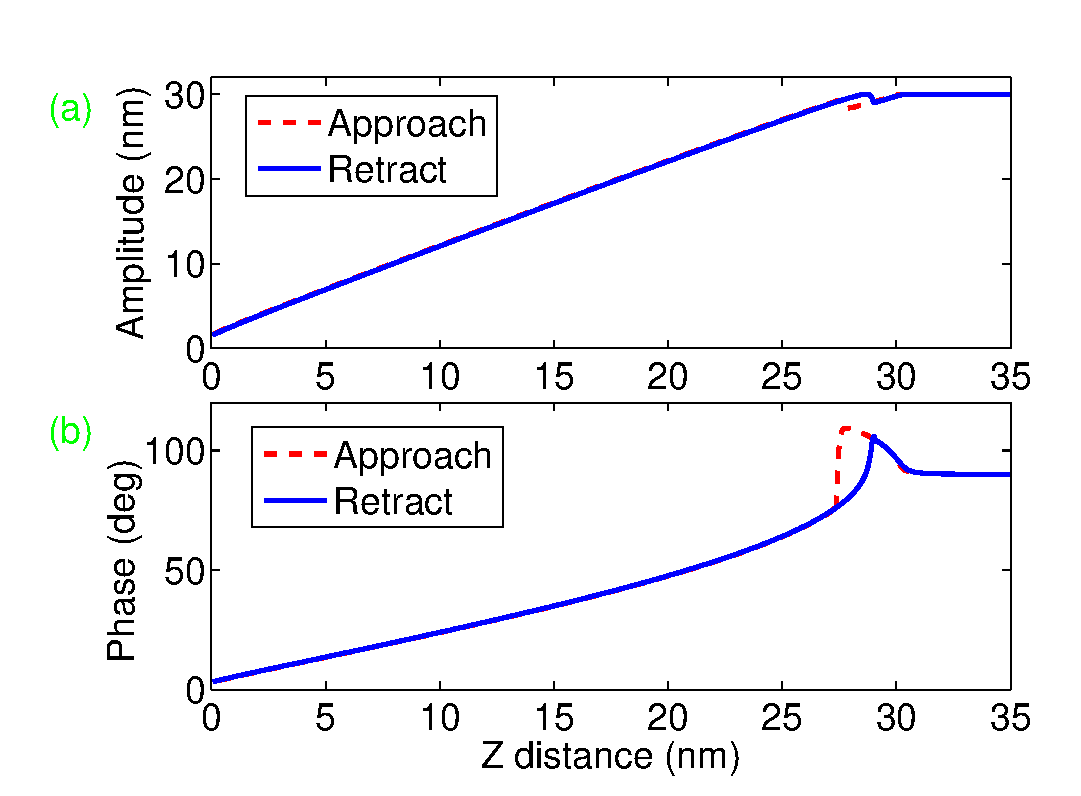
\includegraphics[width=3.5in]{DACex2_A_P} \caption{(a) Amplitude (nm) vs. Z distance for retraction. The jump between
attractive and repulsive regime oscillations occurs at a slightly
different location when retracting from the sample. (b) Phase (deg)
vs. Z distance for retraction from the sample. (\textbf{AMAC} Example
2)}
\par\end{centering}
\centering{}\label{fig:DACex2_A_P} 
\end{figure}

The results of the retraction simulation are shown in Figures \ref{fig:DACex2_A_P}-\ref{fig:DACex2_C}.
We find that there is noticeable amplitude and phase hysteresis for
Z distances between 27 to 30 nm. If the simulations for approaching
the sample and retracting from the sample are performed successively,
the user will be able to plot both sets of results for comparison.
We encourage users who are interested in hysteresis to download the
actual data for plotting purposes.

\begin{figure}[htp]
\begin{centering}
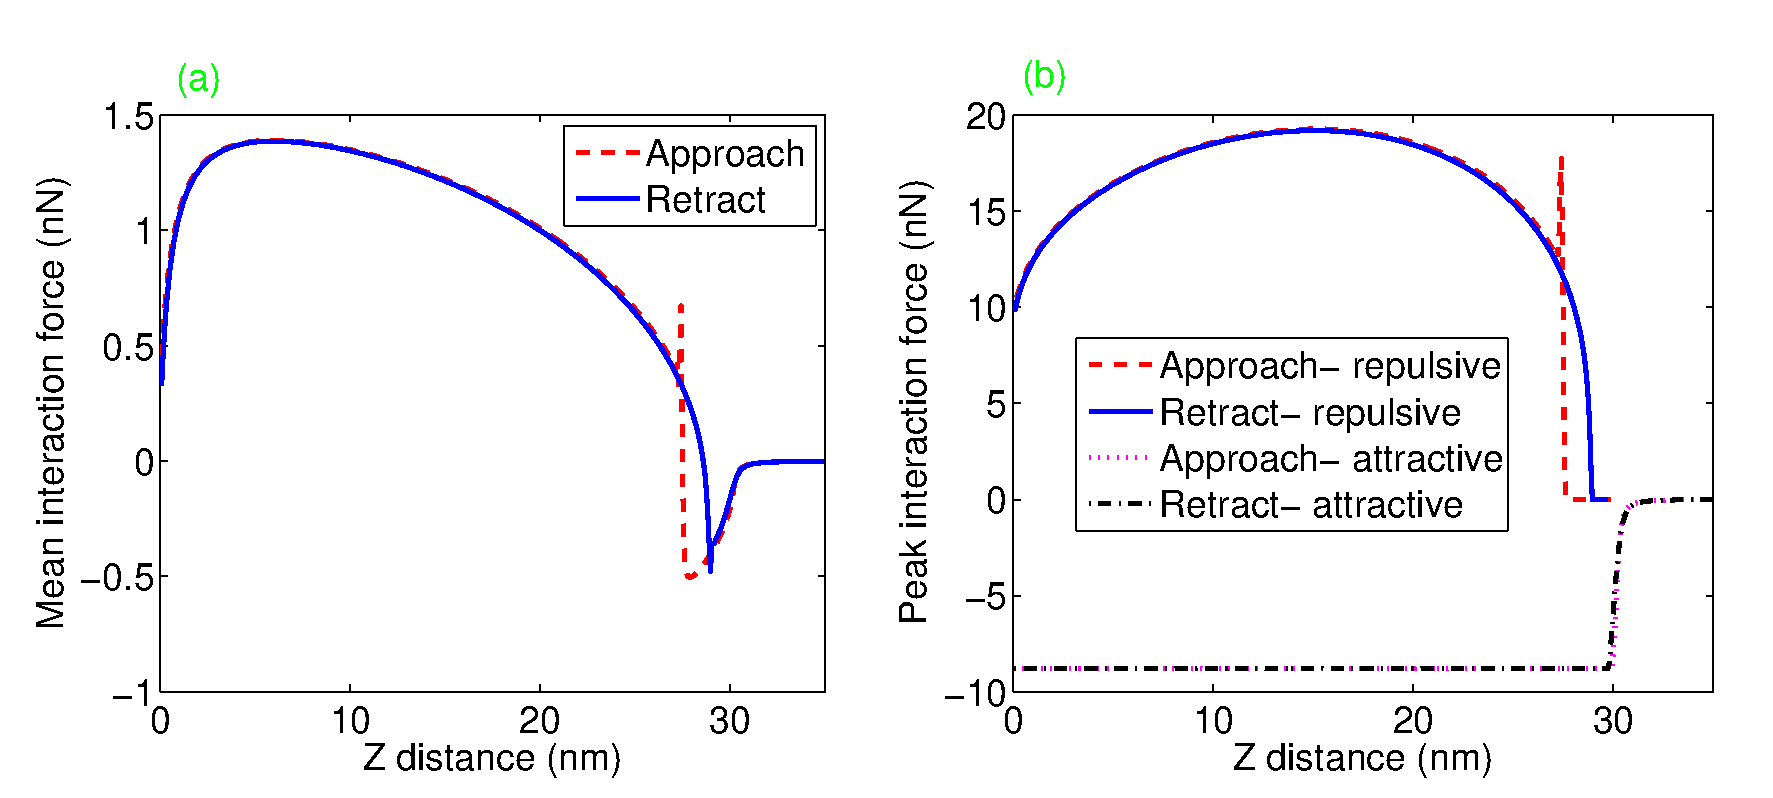
\includegraphics[width=6in]{DACex2_Mf_Pf} \caption{(a) Mean interaction force (nN) vs. Z distance (nm) while retracting
from the sample. (b) Peak attractive and repulsive interaction forces
(nN) vs. Z distance (nm) while retracting from the sample. (\textbf{AMAC}
Example 2)}
\par\end{centering}
\centering{}\label{fig:DACex2_Mf_Pf} 
\end{figure}

\emph{Important note:} For these operating parameters there is a range
of Z distances where there are two amplitude branches, hence the hysteresis.
If the user is interested in studying approach/retraction hysteresis,
the cantilever must start in the repulsive regime during retraction
curves and the attractive regime during approach. In this simulation,
the initial Z separation was chosen to be 0 assuring with a high degree
of confidence that the cantilever will start in the repulsive regime.
This is confirmed in Figure \ref{fig:DACex2_Mf_Pf}. Had we chosen
an initial Z separation closer to 25 nm, where there are two amplitude
branches, this may not have been the case.

\begin{figure}[htp]
\begin{centering}
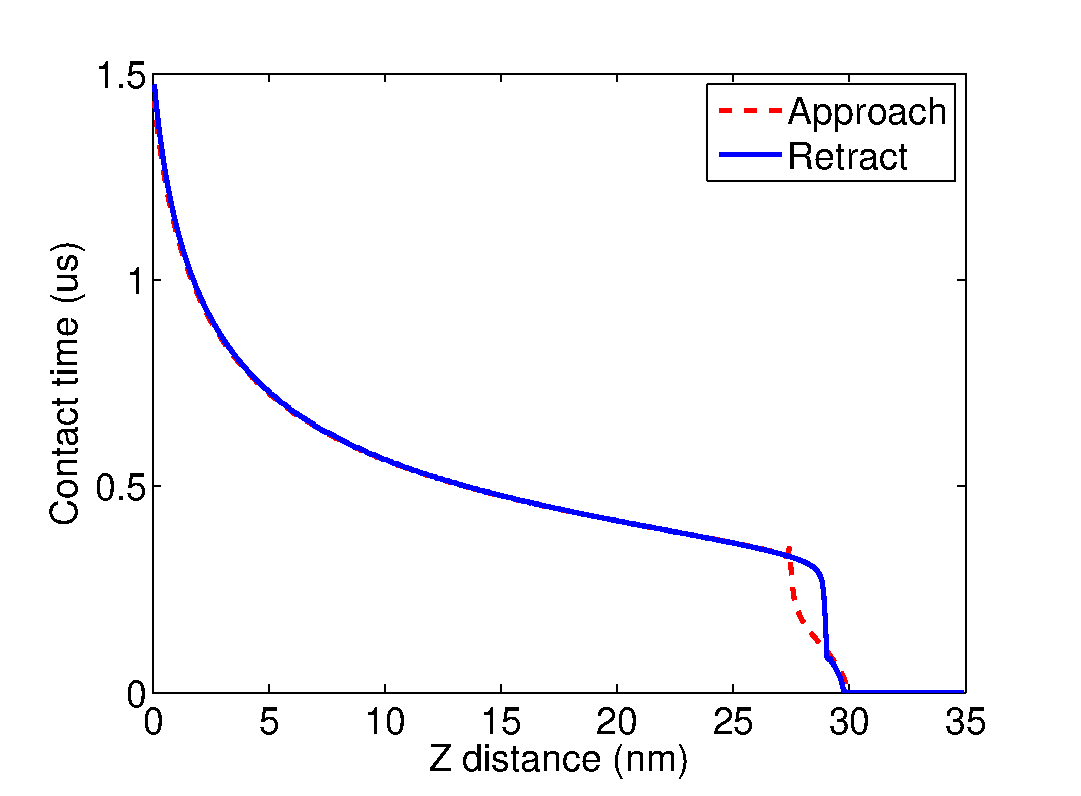
\includegraphics[width=3.5in]{DACex2_C} \caption{Contact time ($\mu s$) vs. Z distance (nm) while retracting from
the sample. (\textbf{AMAC} Example 2)}
\par\end{centering}
\centering{}\label{fig:DACex2_C} 
\end{figure}



\subsubsection{\label{sec:Tools.DAC.Ex3}Example 3: Effects of viscoelastic damping
in polymer samples}


Our final example focuses on the effects of sample viscoelastic damping
on the amplitude modulated approach curves and the resulting power
dissipation curve resulting from this particular form of non-conservative
tip-sample interaction. For this simulation, we choose sample properties
that are characteristic of typical polymers including a sample viscosity
of 500 Pa s (Table \ref{tab:DACEx}).

To begin this example, open the \textbf{AMAC} tool from the \textbf{VEDA}
tools selection. Wait for the user input window to open. Under the
\emph{Operating conditions and cantilever properties} tab, set the
\emph{Unconstrained amplitude (nm)} to 60, and set \emph{$k_{i}$
(N/m)} to 3. Change \emph{Q} to 150, change both \emph{f (kHz)} and
\emph{$f_{d}$ (kHz)} to 75, and change \emph{Z approach velocity
(nm/s)} to 500. Next, click the \emph{Tip-sample interaction properties}
tab. Under this tab, be sure that the \emph{Tip-sample interaction
model} is \emph{Hertz contact}. At the bottom under ``non-conservative
forces'', change ``Include sample viscoelastic forces'' to the
``Kelvin-voigt'' model. Change the rest of the input parameters
under this tab and under the \emph{Simulation parameters} tab to match
those shown in Table \ref{tab:DACEx} Example 3. Once all of the inputs
have been correctly modified, click the \emph{Simulate} button in
the lower right-hand corner. This simulation generally takes about
1.25 minutes to run to completion. After the simulation is finished,
click back to tab 2 and change the ``Include sample viscoelastic
forces'' to ``None''. Run this simulation and then compare the
results with and without the viscoelastic forces.

The results of this simulation are shown in Figures \ref{fig:DACex3_A_P}
- \ref{fig:DACex3_I_C}.

First, in Fig. \ref{fig:DACex3_A_P}, we see that the amplitude does
not change very much with the addition of the viscoelastic forces,
but the phase changes significantly. The change in phase can be related
to the fact that viscoelastic forces are non-conservative. That is,
they dissipate energy. This is seen in Fig. \ref{fig:DACex3_Mf_Pf_Wdot}.
Additional effects of the viscous interaction are seen in the mean
(Figure \ref{fig:DACex3_Mf_Pf_Wdot}a) and peak (Figure \ref{fig:DACex3_Mf_Pf_Wdot}b)
interaction forces. The viscoelasticity significantly raises the peak
force, although the mean force decreases slightly.

To have a better look at the forces, we can examine the interaction
force time histories shown in Figure \ref{fig:DACex3_D_TS}. During
most of the cycle, the tip is not in contact with the sample. This
figure shows just the small portion where they are in contact. Again,
the peak value of the force is higher with the viscoelasticity, although
the total area under the curve (the mean force) is approximately the
same. Most notable, the shape of the force curve is asymmetric due
to the viscous contribution.

Many additional details about viscoelasticity can be found under the
viscoelasticity part of the theory section of this manual.

\begin{figure}[htb]
\begin{centering}
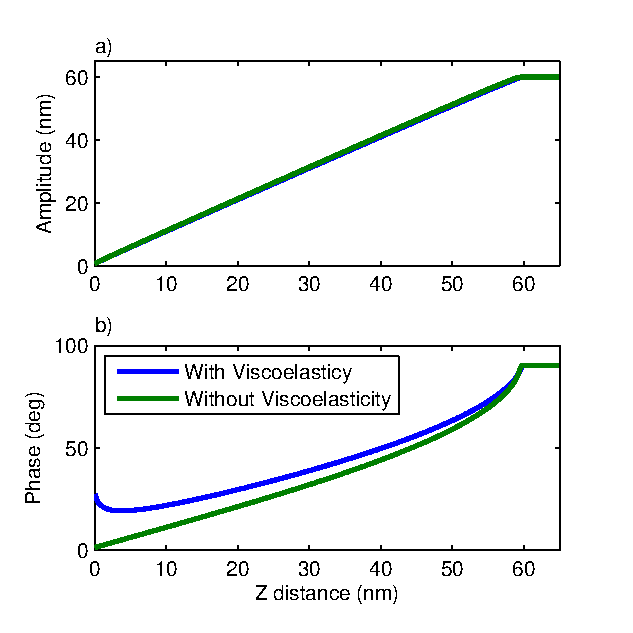
\includegraphics[width=3.5in]{DACex3_A_P} \caption{(a) Amplitude (nm) vs. Z distance. (b) Phase (deg) vs. Z distance.(\textbf{AMAC}
Example 3).}
\par\end{centering}
\centering{}\label{fig:DACex3_A_P} 
\end{figure}

\begin{figure}[htb]
\begin{centering}
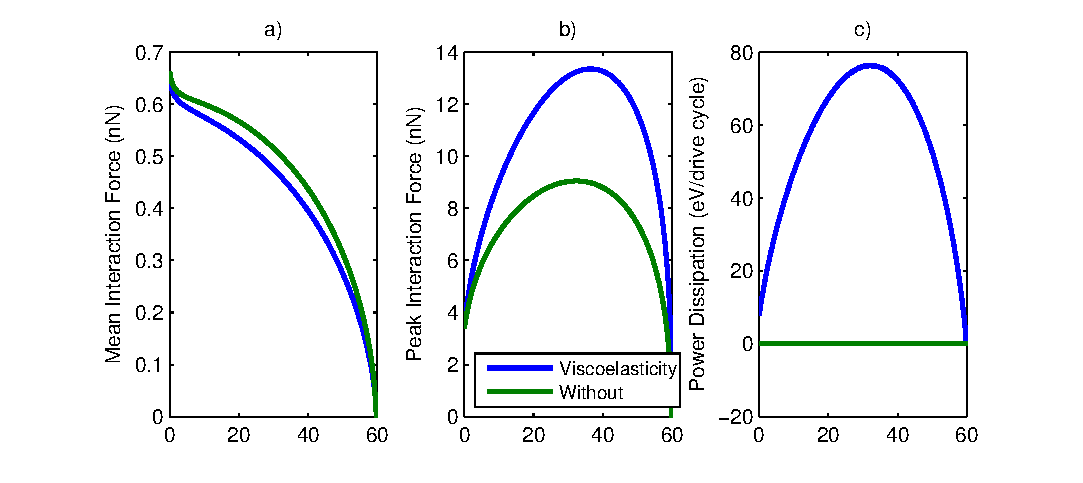
\includegraphics[width=6in]{DACex3_Mf_Pf_Wdot} \caption{(a) Mean interaction force (nN) vs. Z distance. (b) Peak interaction
force (nN) vs. Z distance. (c) Power dissipated (pW) vs. Z distance.
The power dissipated by viscoelastic damping depends on both the indentation
and rate of indentation (\textbf{AMAC} Example 3).}
\par\end{centering}
\centering{}\label{fig:DACex3_Mf_Pf_Wdot} 
\end{figure}

\begin{figure}[htb]
\begin{centering}
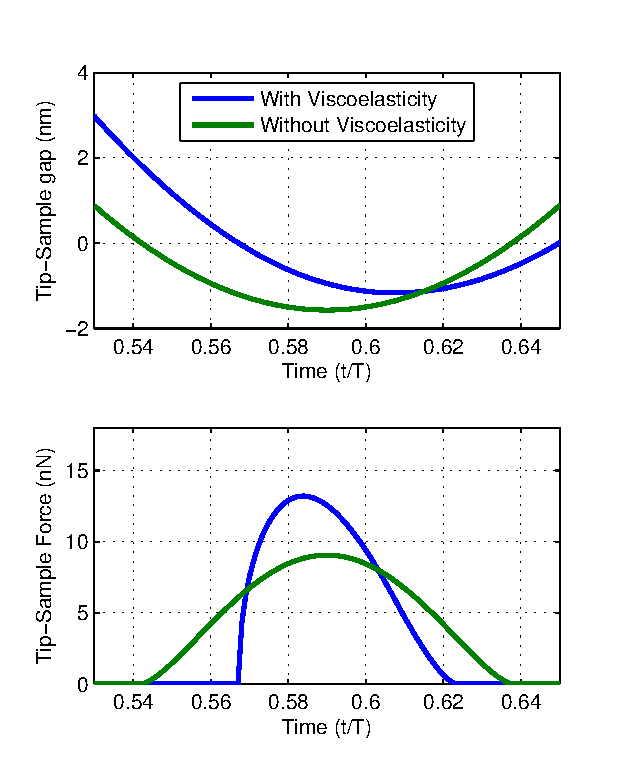
\includegraphics[width=4in]{DACex3_D_TS} \caption{Tip-sample gap and interaction force histories corresponding to $A/A_{0}=0.55$.
The viscoelastic forces cause the interaction force history to be
asymmetric. (\textbf{AMAC} Example 3).}
\par\end{centering}
\centering{}\label{fig:DACex3_D_TS} 
\end{figure}

\begin{figure}[htb]
\begin{centering}
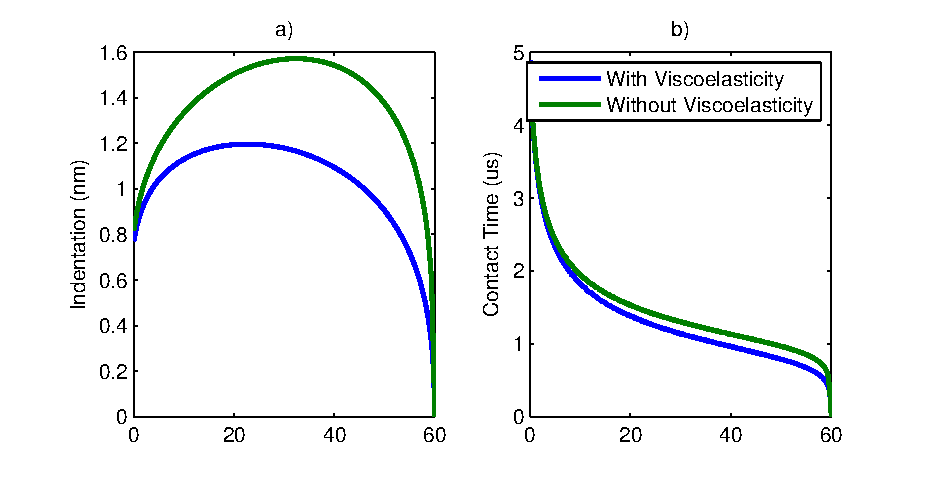
\includegraphics[width=4in]{DACex3_I_C} \caption{(a) Indentation (nm) vs. Z distance (nm). (b) Contact time ($\mu s$)
vs. Z distance (nm). (\textbf{AMAC} Example 3)}
\par\end{centering}
\centering{}\label{fig:DACex3_I_C} 
\end{figure}

\newpage{}



\subsection{\label{sec:Tools.AMS}Amplitude Modulated Scanning (basic)}

A microcantilever is commonly used to image nano-scale surfaces by
tapping along the surface while monitoring the location of the cantilever
base as well as the tip deflection amplitude. The Amplitude Modulated
Scanning tool (AMS) was created to simulate the response of a microcantilever
excited near its first flexural natural frequency and in contact with
a sample while being moved along the surface of the sample as a controller
attempts to keep the cantilever tip deflection amplitude constant.

The following assumptions are unique to the basic Amplitude Modulated
Scanning tool: 
\begin{enumerate}
\item Cantilever dynamics are modeled by a single eigenmode model (Eq. \ref{eq:ndmdof},
$i=1$). 
\item The cantilever is acoustically or magnetically excited with a single
frequency. 
\item The $Z$ separation between the sample can be reduced or increased,
but the cantilever does not move laterally. 
\item The AFM controller is modeled as a simple proportional-integral (PI)
controller. 
\item Inertial and hydrodynamic forces acting on the cantilever due to the
controller's Z adjustment of the base while scanning are negligible. 
\end{enumerate}
This section provides an overview of the outputs of the basic Amplitude
Modulated Scanning (AMS) tool in the form of several example simulations.
\begin{table}[H]
\caption{\label{tab:AMSEx}Input parameters for AMS examples.}

\begin{ruledtabular} %
\begin{tabular}{lrrrrr}
~~~~\textbf{PARAMETER} & \textbf{EX. 1} & \textbf{EX. 2} & \textbf{EX. 3} & \textbf{EX. 4} & \textbf{EX. 5}\tabularnewline
~ &  &  &  &  & \tabularnewline
\textbf{Operating cond. + Cantilever prop.} &  &  &  &  & \tabularnewline
~~~~Choose excitation source & Acoustic & Acoustic & Acoustic & Acoustic & Acoustic\tabularnewline
~~~~Unconstrained Amplitude (nm) & 30 & 30 & 13 & 10 & 6\tabularnewline
~~~~$k$ (N/m) & 40 & 1 & 0.3 & 0.3 & 1\tabularnewline
~~~~$Q$ & 400 & 200 & 100 & 100 & 10\tabularnewline
~~~~$f$ (kHz) & 350 & 30 & 150 & 150 & 40\tabularnewline
~~~~$f_{d}$ (kHz) & 350 & 350 & 150 & 150 & 40\tabularnewline
~~~~Tip mass, ($m_{tip}/m_{c}$) & 0 & 0 & 0 & 0 & 0\tabularnewline
~~~~Set point ratio & 0.9 & 0.9 & 0.98 & 0.85 & 0.7\tabularnewline
~~~~Signal/Noise ratio (dB) & 20 & 80 & 30 & 30 & 60\tabularnewline
~~~~Scan Lines per second & 13.33 & 33.33 & 33.33 & 33.33 & 10\tabularnewline
~~~~Proportional gain & 0.002 & 0.002 & 0.008 & 0.001 & 0.04\tabularnewline
~~~~Integral gain & 0.002 & 0.0015 & 0.004 & 0.004 & 0.1\tabularnewline
~~~~Sampling frequency (Mhz) & 1 & 1 & 1 & 1 & 1\tabularnewline
~~~~Lock-in filter order & 2nd & 2nd & 2nd & 2nd & 2nd\tabularnewline
~~~~Lock-in time constant ($\mu s$) & 50 & 50 & 50 & 50 & 200\tabularnewline
~ &  &  &  &  & \tabularnewline
\textbf{Tip-sample int. prop: substrate} &  &  &  &  & \tabularnewline
~~~~Tip-sample interaction model & DMT contact & DMT contact & DMT contact & DMT contact & Hertz\tabularnewline
~~~~Tip radius (nm) & 10 & 10 & 10 & 10 & 10\tabularnewline
~~~~Young's modulus of tip (GPa) & 130 & 130 & 130 & 130 & 130\tabularnewline
~~~~Poisson's ratio of the tip & 0.3 & 0.3 & 0.3 & 0.3 & 0.3\tabularnewline
~~~~Auto Calculate intermolecular distance? & yes & yes & no & yes & NA\tabularnewline
~~~~van der Waals Adhesion force (nN) & 3.2 & 3.4 & N/A & 1.4 & NA\tabularnewline
~~~~Intermolcular distance (nm) & N/A & N/A & 0.2 & N/A & NA\tabularnewline
~~~~Hamaker constant (J) & $1.8\cdot10^{-19}$ & $2.96\cdot10^{-19}$ & $3.4\cdot10^{-20}$ & $3.4\cdot10^{-20}$ & NA\tabularnewline
~~~~Young's modulus of sample (GPa) & 130 & 10 & 60 & 60 & 1\tabularnewline
~~~~Poisson's ratio of the sample & 0.3 & 0.3 & 0.3 & 0.3 & 0.3\tabularnewline
~~~~Include sample visco-elastic forces & None & 3 element & None & None & None\tabularnewline
~~~~Sample E2 modulus (GPa) & NA & 0.1 & NA & NA & NA\tabularnewline
~~~~Sample Viscosity ($Pa\cdot s$) & NA & 100 & NA & NA & NA\tabularnewline
~ &  &  &  &  & \tabularnewline
\textbf{Simulation parameters} &  &  &  &  & \tabularnewline
~~~~Number of points plotted & 1000 & 1000 & 1000 & 1000 & 1000\tabularnewline
~~~~Maximum number of deflection points per cycle & 1000 & 1000 & 1000 & 1000 & 1000\tabularnewline
~~~~Scan size (length) (nm) & 150 & 30 & 30 & 30 & 100\tabularnewline
~ &  &  &  &  & \tabularnewline
\textbf{Feature properties} &  &  &  &  & \tabularnewline
~~~~Select a geometric feature & Trapezoid & Step & Step & Step & Step\tabularnewline
~~~~Feature height (nm) & -40 & 0 & 1 & 1 & 0\tabularnewline
~~~~Length of feature (nm) & 110 & 10 & 10 & 10 & 50\tabularnewline
~~~~Length of trapezoid top (nm) & 50 & NA & NA & NA & NA\tabularnewline
~~~~Include geometric convolution & no & no & no & no & no\tabularnewline
~~~~Specify material properties & no & yes & yes & no & yes\tabularnewline
~~~~Tip-sample interaction model & NA & DMT contact & DMT contact & NA & DMT contact\tabularnewline
~~~~Auto Calculate intermolecular distance? & NA & yes & no & NA & yes\tabularnewline
~~~~Intermolecular distance & NA & NA & 0.2 & NA & NA\tabularnewline
~~~~van der Waals Adhesion force (nN) & NA & 4.4 & N/A & NA & 15\tabularnewline
~~~~Hamaker constant (J) & NA & $7.1\cdot10^{-20}$ & $3.0\cdot10^{-20}$ & NA & 1e-19\tabularnewline
~~~~Young's modulus of sample (GPa) & NA & 1.2 & 60 & NA & 1\tabularnewline
~~~~Poisson's ratio of the sample & NA & 0.3 & 0.3 & NA & 0.3\tabularnewline
~~~~Include sample visco-elastic forces & None & 3 element & None & None & None\tabularnewline
~~~~Feature E2 modulus (GPa) & NA & 0.1 & NA & NA & NA\tabularnewline
~~~~Feature Viscosity ($Pa\cdot s$) & NA & 10 & NA & NA & NA\tabularnewline
\end{tabular}\end{ruledtabular} 
\end{table}


\subsubsection{\label{sec:Tools.AMS.Ex1}Example 1: Silicon trench}

In the first example, we choose to simulate an amplitude modulated
AFM scan of a silicon trench, representing a critical feature of a
semiconductor device.

Prior to performing the scanning simulation, we first explore the
dynamics between the cantilever probe and the sample with the Amplitude
Modulated Approach Curves tool. The necessary inputs for this simulation
are all also present in Table \ref{tab:AMSEx} with the exception
of the Z approach velocity, which was chosen as 200 nm/s. To begin
this example, open the \textbf{AMAC} tool from the \textbf{VEDA} tools
selection. Enter the proper user inputs as shown in the Table \ref{tab:AMSEx},
then click the \emph{Simulate} button in the lower right-hand corner.
After this simulation is complete, open the \textbf{AMS} tool from
the \textbf{VEDA} tools selection. After the user input window has
opened, change the input values to those shown in Table \ref{tab:AMSEx},
and click the \emph{Simulate} button in the lower right-hand corner.

From the results of AMAC simulation (Figure \ref{fig:AMS_Ex1_dac_A_P}),
we find that the transition from attractive to repulsive regime is
more subtle (See Example 1 (\ref{sec:Tools.DAC.Ex1}) of AMAC for
a contrasting example). To ensure that the cantilever will be tapping
on the sample at the chosen set point ratio, we look at the phase
vs. Z distance curve (Figure \ref{fig:AMS_Ex1_dac_A_P}). When exciting
the cantilever at resonance, a negative phase shift confirms that
the cantilever is oscillating in the repulsive regime or ``tapping''
on the sample as long as the interaction is conservative. Finally,
larger set point ratios are generally preferred to reduce peak repulsive
interaction forces (Figure \ref{fig:AMS_Ex1_dac_Pf}). With this in
mind, we choose a set point ratio of 0.90 for this simulation. 
\begin{figure}[htb]
\begin{centering}
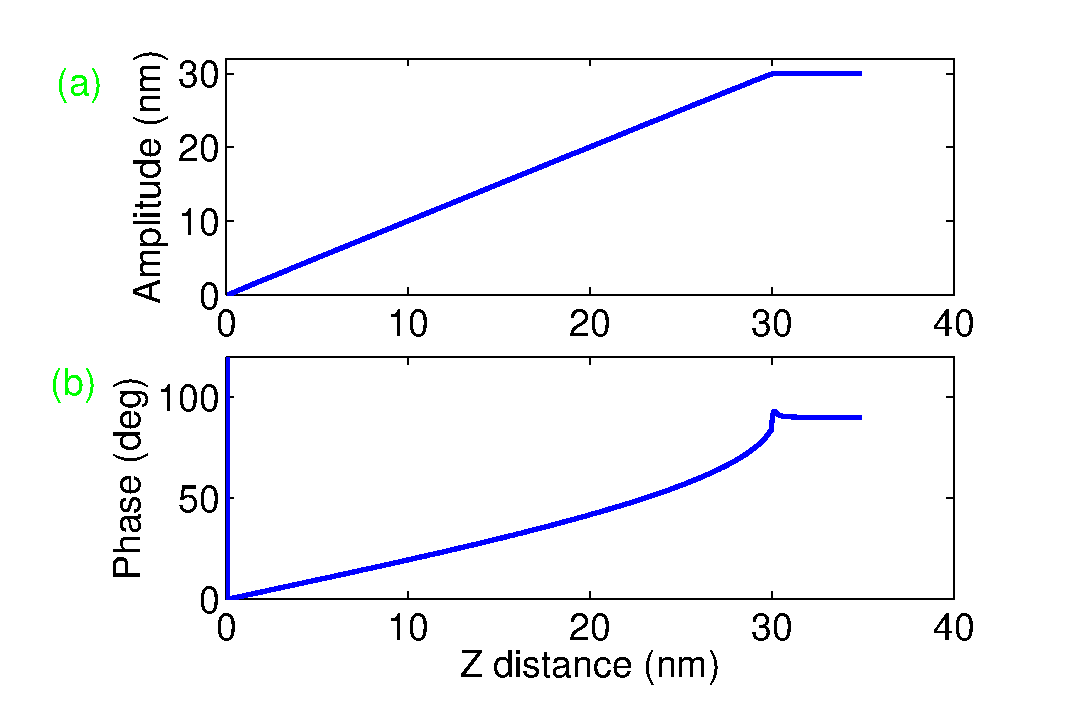
\includegraphics[width=3.5in]{AMS_Ex1_dac_A_P} \caption{(a) Amplitude (nm) vs. Z distance (b) Phase (deg) vs. Z distance (nm).
(\textbf{AMS} Example 1)}
\par\end{centering}
\centering{}\label{fig:AMS_Ex1_dac_A_P} 
\end{figure}

\begin{figure}[htb]
\begin{centering}
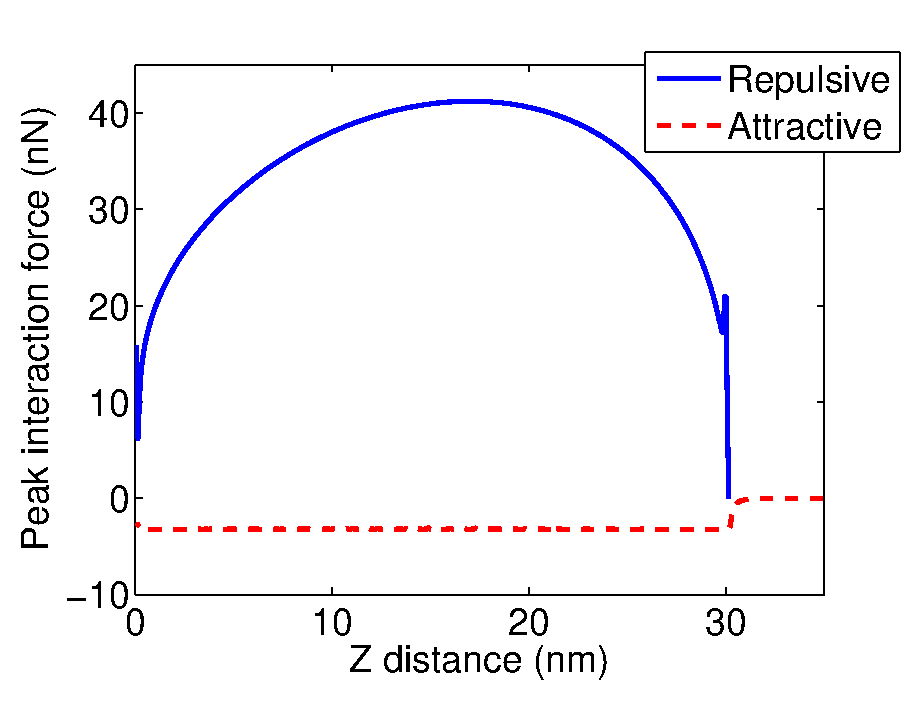
\includegraphics[width=3.5in]{AMS_Ex1_dac_Pf} \caption{Peak repulsive and attractive interaction forces (nN) vs. Z distance
(nm). (\textbf{AMS} Example 1)}
\par\end{centering}
\centering{}\label{fig:AMS_Ex1_dac_Pf} 
\end{figure}

Next, we need to determine the proportional gain and integral gain
of the controller. To do so, we can apply the following methodology.
The default gains should provide a good starting point, however these
values may need to be adjusted for different cantilever and tip-sample
properties and lock-in time constant. In general, if the system is
unstable, or if there is a large ringing effect, these gains should
be decreased. If the system is stable and there is no ringing, then
these gains may be increased if there is a slow response time. Note
that the controller is active during the transient computations so
if the simulation progress bar stays on transient for a very long
time, you may have an unstable controller and should probably decrease
your gains.

Through some experimentation, we choose 0.002 as the proportional
gain and 0.002 as the integral gain. Finally, the sample geometry
is constructed by choosing the trapezoidal feature type and entering
a negative feature height. All other inputs for this example are shown
in Table \ref{tab:AMSEx}.

The results of the scanning simulation are shown in Figures \ref{fig:AMS_Ex1_H_P}
- \ref{fig:AMS_Ex1_I}. The measured topography (Figure \ref{fig:AMS_Ex1_H_P}a)
refers to the sample height imaged by the AFM. This is determined
by first allowing the simulation to reach steady state oscillations
at the specified set point ratio, and then as the cantilever begins
to scan over the sample and the change in Z distance based on the
lock-in (Eq. \ref{eq:cont}) is recorded as the sample topography.
The measurement error (Figure \ref{fig:AMS_Ex1_Merr_Aerr}) represents
the difference between the actual sample height and the measured topography.
The amplitude error (Figure \ref{fig:AMS_Ex1_Merr_Aerr}) represents
the difference between the computed amplitude and the amplitude that
satisfies the set point ratio. The amplitude is calculated two ways.
First, by the lock-in and second by a Fourier transform. The controller
uses the lock-in's calculation, the Fourier transform is provided
as a reference so that you can check the performance of the lock-in.
The phase (Figure \ref{fig:AMS_Ex1_H_P}) is computed is the same
manner. Finally, the mean and peak interaction forces (Figure \ref{fig:AMS_Ex1_Mf_Pf})
and indentation (Figure \ref{fig:AMS_Ex1_I}) are found from the tip
oscillation waveform (without noise).

\begin{figure}[htb]
\begin{centering}
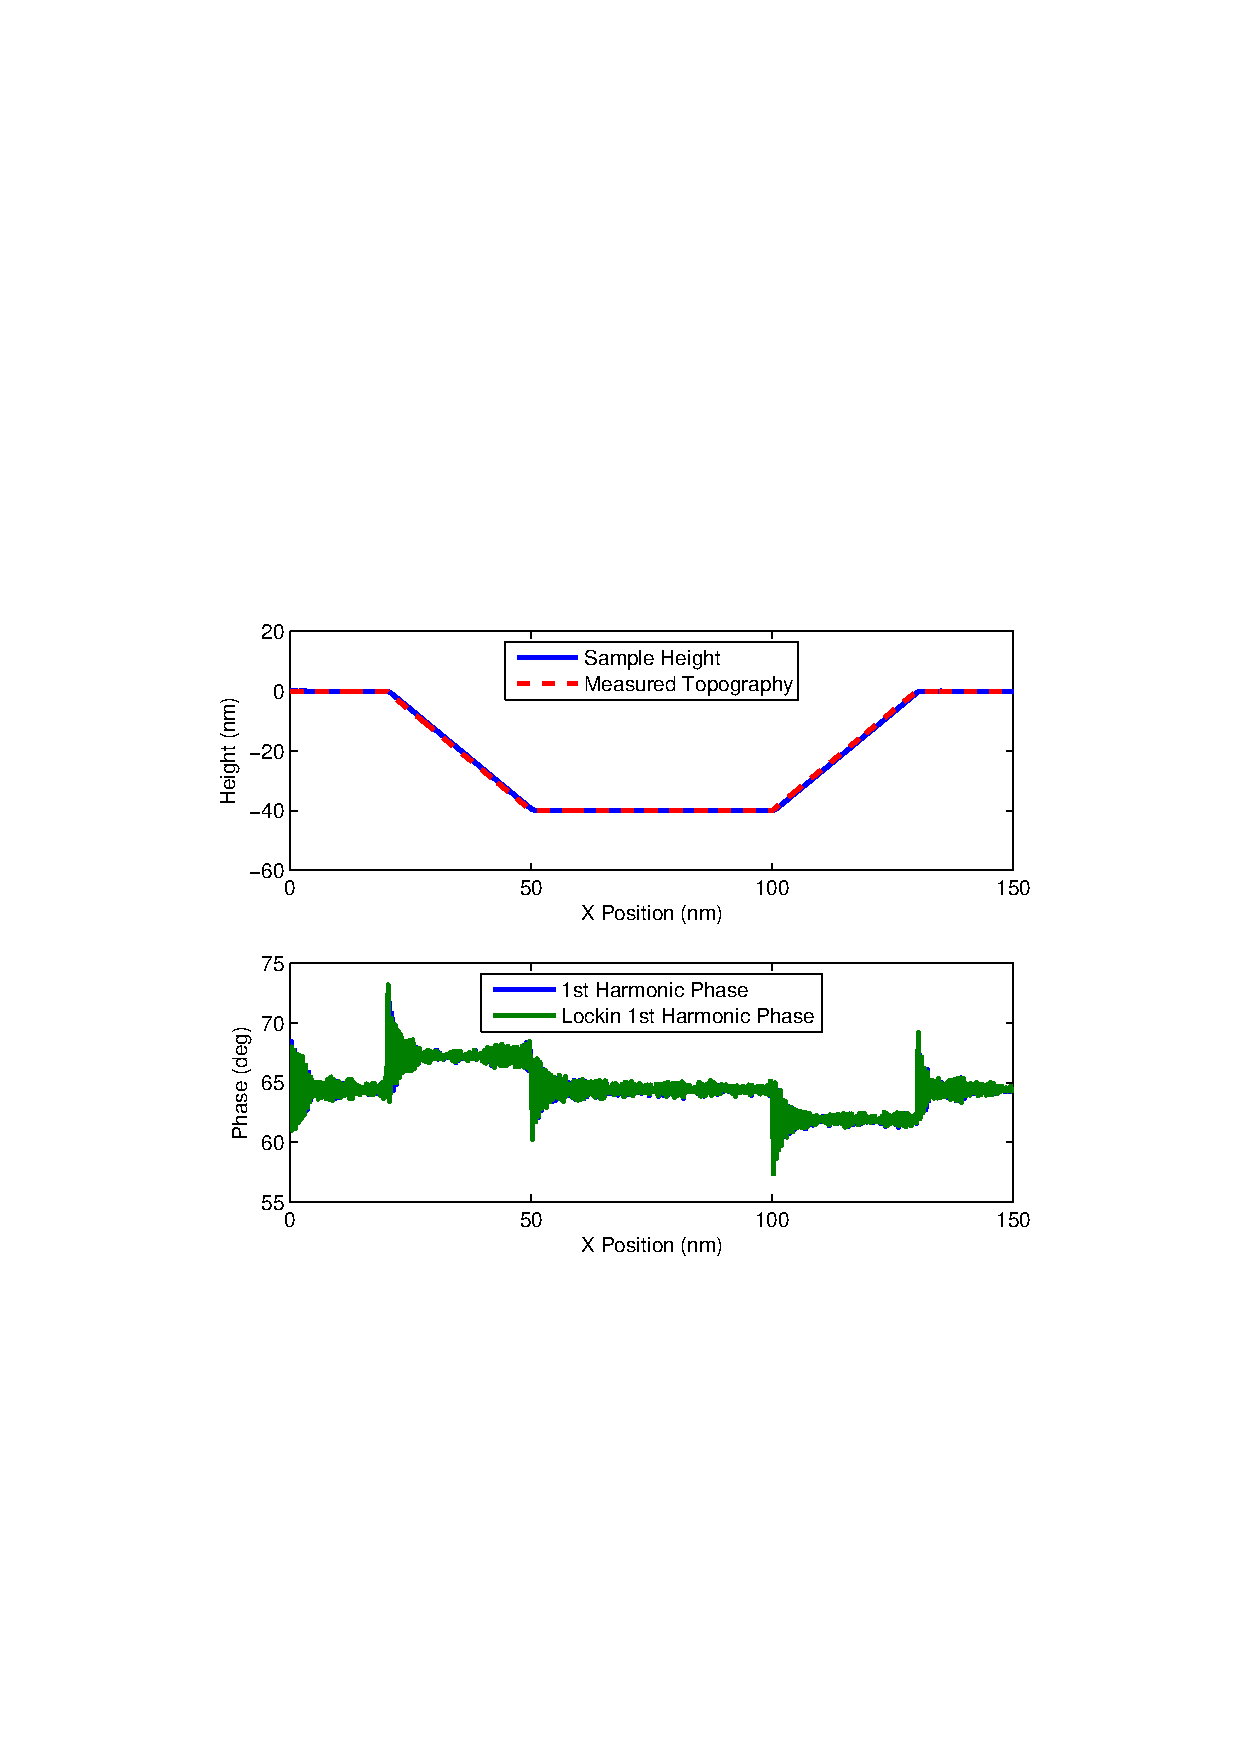
\includegraphics[clip,width=4.5in]{AMS_Ex1_H_P} \caption{(top) Measured topography and true sample height vs. X distance (nm)
over which the AFM scans. (bottom) The phase (deg) vs. X distance
(nm). (\textbf{AMS} (basic) Example 1)}
\par\end{centering}
\centering{}\label{fig:AMS_Ex1_H_P} 
\end{figure}

\begin{figure}[htb]
\begin{centering}
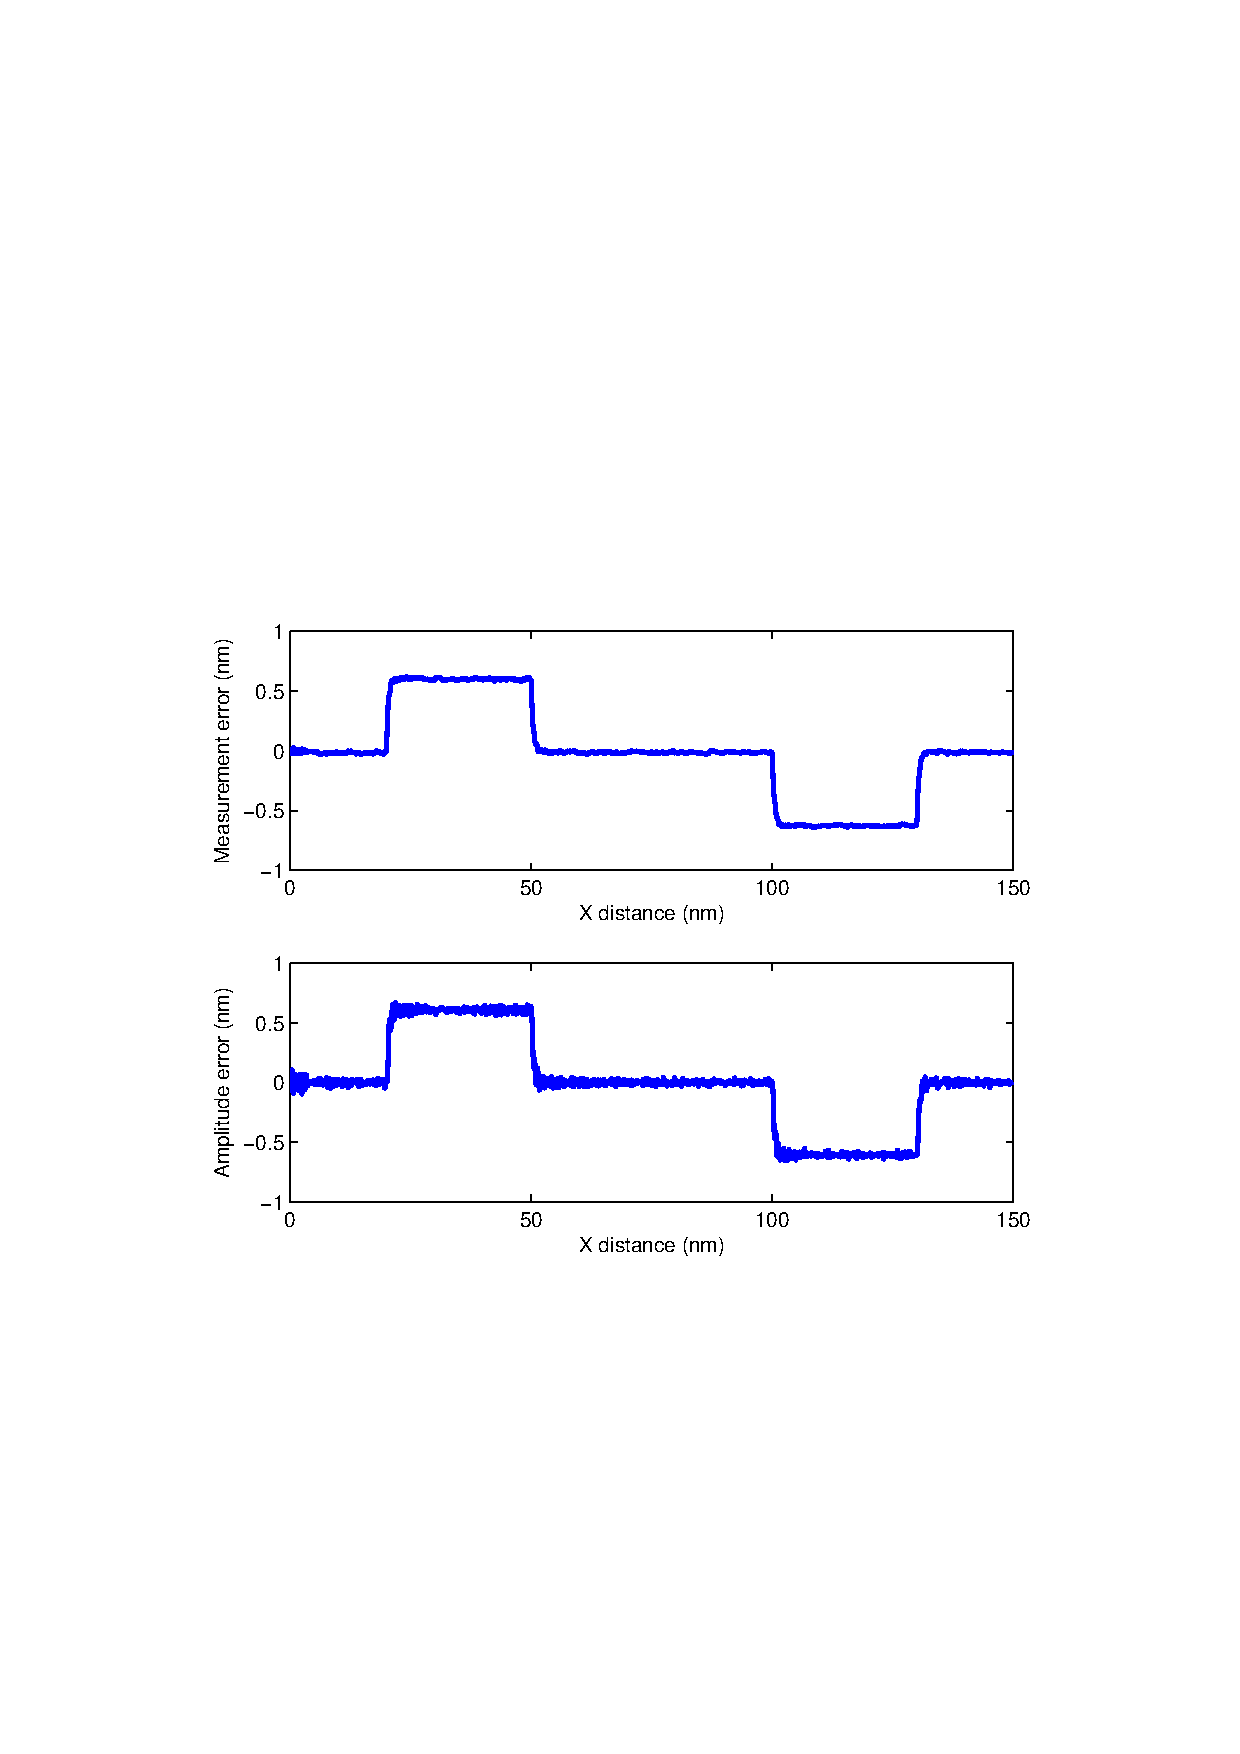
\includegraphics[clip,width=4.5in]{AMS_Ex1_Merr_Aerr} \caption{(a) The measurement error (nm) vs. X distance (nm) plotted represents
the difference between the measured topography and the sample height
(see Figure \ref{fig:AMS_Ex1_H_P}). (b) Amplitude error (nm) vs.
X distance (nm). The amplitude error is defined in Eq. \ref{error}
and differs from the measurement error due to the integral feedback
term (Eq. \ref{eq:cont}). (\textbf{AMS} Example 1)}
\par\end{centering}
\centering{}\label{fig:AMS_Ex1_Merr_Aerr} 
\end{figure}

\begin{figure}[htb]
\begin{centering}
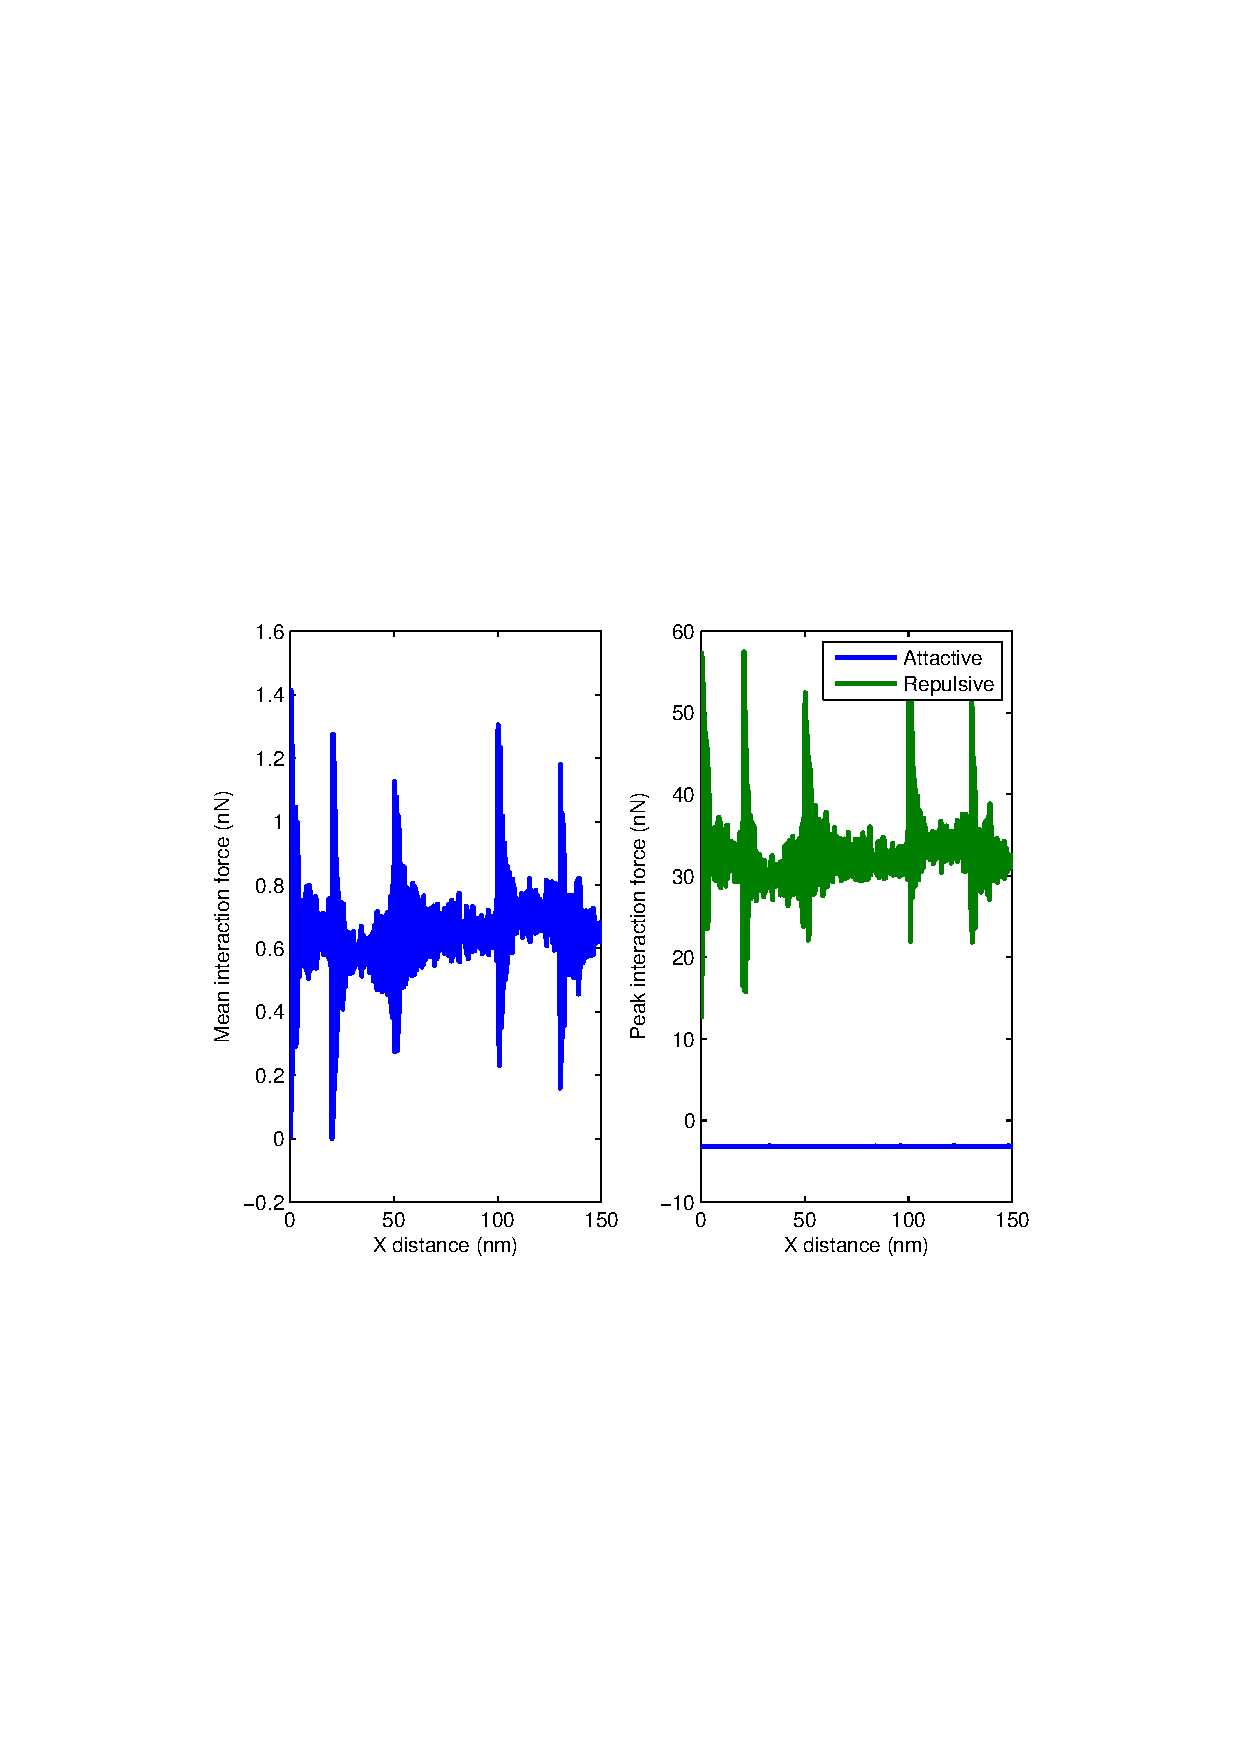
\includegraphics[clip,width=4.5in]{AMS_Ex1_Mf_Pf} \caption{(a) The mean interaction force (nN) vs. X distance (nm) is calculated
based on the clean, padded tip oscillation waveform. (b) Peak attractive
and repulsive interaction forces (nN) vs. X distance. Peak forces
are calculated based on the clean tip oscillation waveform. (\textbf{AMS}
Example 1)}
\par\end{centering}
\centering{}\label{fig:AMS_Ex1_Mf_Pf} 
\end{figure}

\begin{figure}[htb]
\begin{centering}
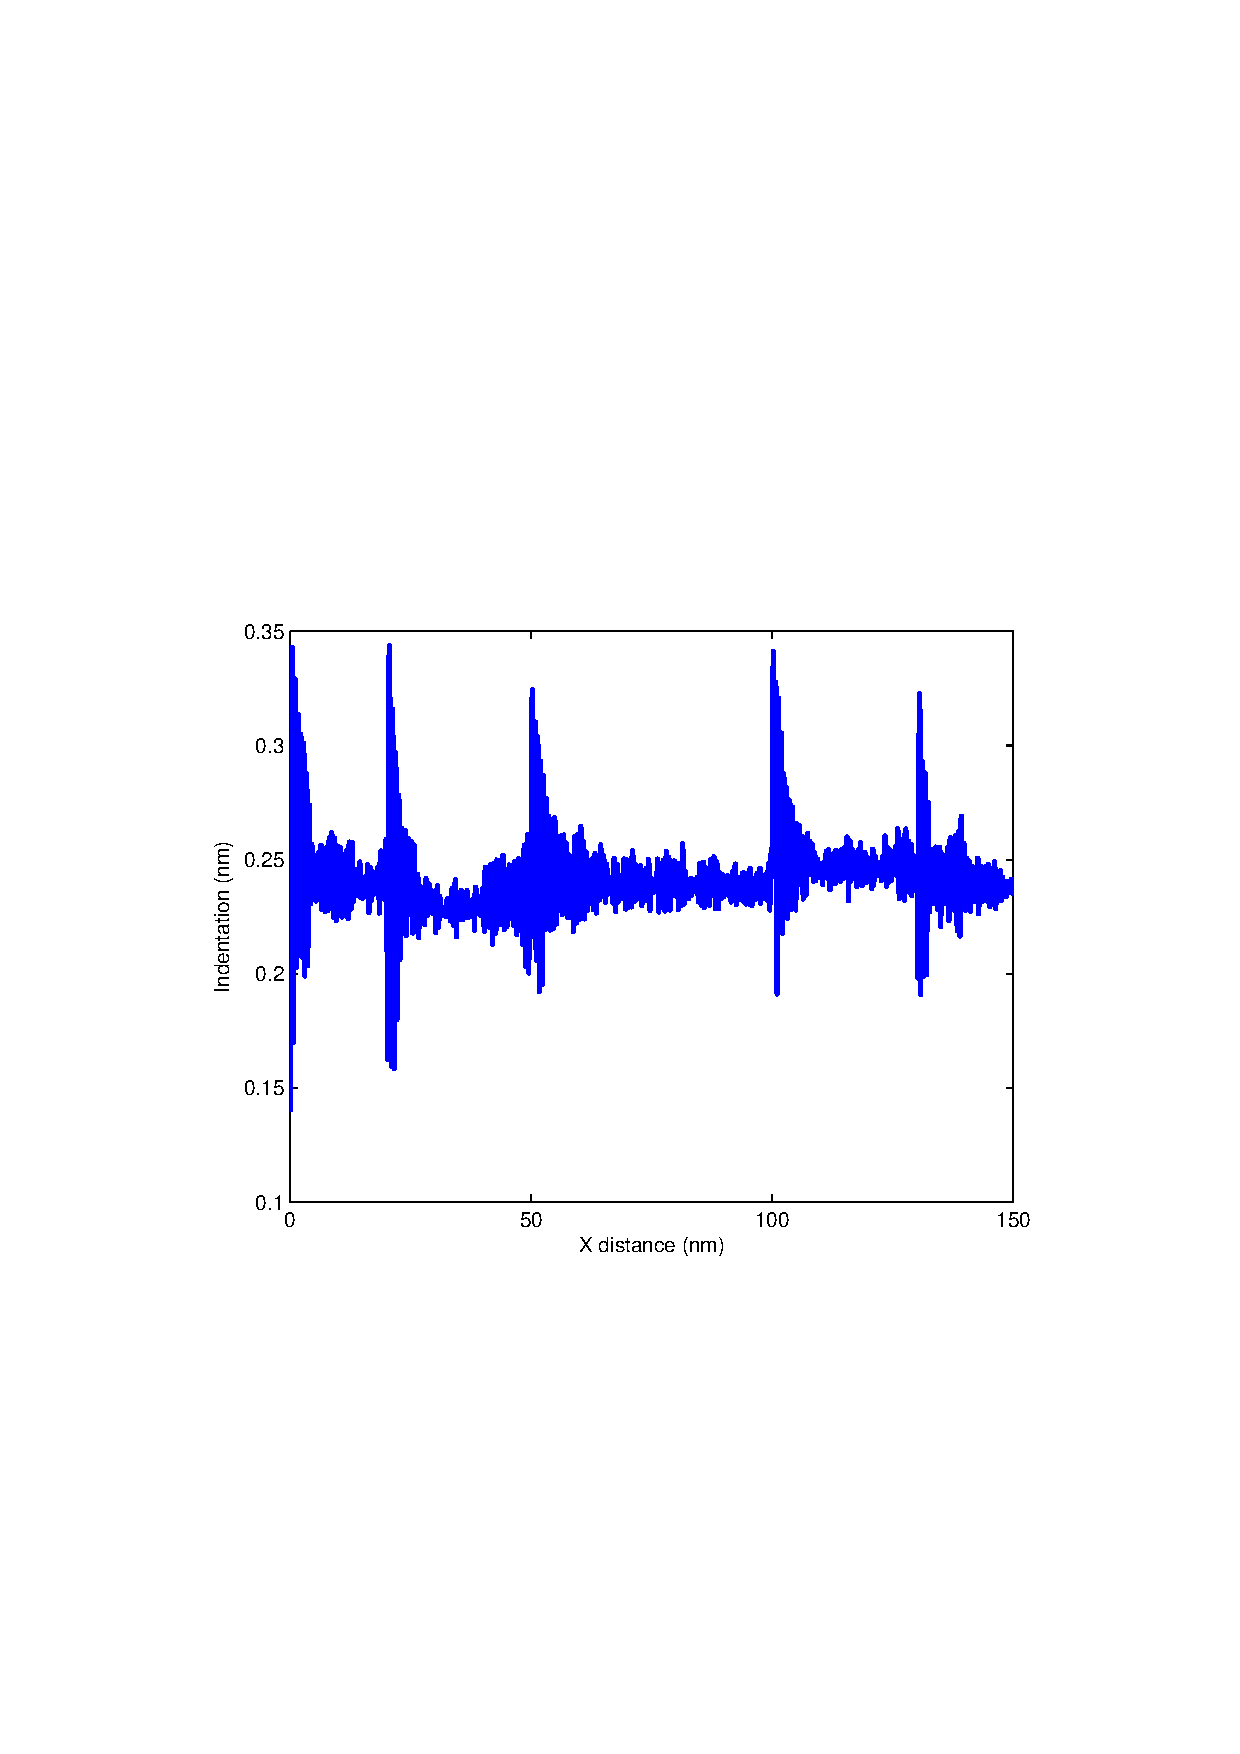
\includegraphics[clip,width=3.5in]{AMS_Ex1_I} \caption{The indentation (nm) vs. X distance (nm) corresponds to the peak repulsive
force for the DMT contact force model. Indentation is calculated from
the clean tip oscillation waveform. (\textbf{AMS} Example 1)}
\par\end{centering}
\centering{}\label{fig:AMS_Ex1_I} 
\end{figure}

\clearpage{}

\subsubsection{\label{sec:Tools.AMS.Ex2}Example 2: Phase contrast in polymer blends}

In this example we simulate scanning over a flat (no change in actual
topography), heterogeneous sample composed of two different polymers.
The total sample is 30 nm long and there is a 10 nm patch in the center
that has different visco-elastic properties than the rest. We choose
a smooth sample (Figure \ref{fig:AMS_Ex2_H_P}) to investigate the
spurious topography imaged by the AFM due to different tip-sample
interaction properties for the two materials. Finally, we choose similar
input parameters as the previous example (Table \ref{tab:AMSEx}),
but with a cleaner signal (60 dB) to reduce measurement error due
to signal noise.

To run this simulation, choose ``Example 2'' from the example loader
drop down box. Looking at the material properties tab for the substrate
versus the feature, we see that we are modeling the contact with a
Hertz contact based model (sec \ref{subsec:Hertz-contact-based})
and modeling the viscoelastic properties with a three element model
(sec \ref{subsec:Three-element-model}) The two modulii $E_{1}$ and
$E_{2}$ are the same, but the viscosity is different. A better understanding
of what this means can be gained by using equations \eqref{eq:Gstorage3elm}
and \eqref{eq:Gloss3elm} to calculate the storage and loss modulus
for each material. This is shown in Figure \label{fig:AMS_ex2_dyn_mod}.
Because $E_{1}$ and $E_{2}$ are the same, the static modulus (i.e.
the modulus that would be probed by a slow F-z curve) are the same,
as are the high frequency behaviors. However, because the viscosity
is not the same, the dynamic behavior at intermediate frequencies
is different. Specifically, near the drive frequency of 30 kHz (dashed
line), the red curve (the feature in the center) is significantly
\emph{softer} than the blue curve (the substrate). The loss modulus
is significantly higher on the blue material, so we expect more energy
dissipation there. 

The results for this simulation are shown in Figure \ref{fig:AMS_Ex2_H_P}-\ref{fig:AMS_Ex2_Mf_Pf_Wdot}.
Figure \ref{fig:AMS_Ex2_H_P} shows the topography imaged by the AFM.
There is a step between the materials, but the sample is actually
flat, so this is a measurement error of around -0.8 nm. Looking as
the indentation (c) we see that there is also a 0.8 nm difference
in indentation and we conclude that the measurement error is largely
due to the difference in indentation of the (dynamically) softer sample.
Thus topography errors can be expected due to changes in local viscoelasticity
of the sample.

If we were to repeat this simulation with a cantilever natural frequency
that was significantly lower, there would be a reverse in phase contrast
because there would be significantly more energy dissipation on the
blue material than on the red. (try it yourself: for example 35 kHz
nat. freq. and drive frequency. Also use a lockin time constant 2
kHz and 3.33 line/s).

There is also clear phase contrast for the two different regions (d).
In particular, the red material has a lower phase. This corresponds
to less energy dissipation on the red material, as expected from the
lower loss tangent at the driving frequency. 

This simulation was relatively straighforward. Now let us repeat the
simulation for a case that is not so easy to interpret. Increase the
natural frequency and driving frequency to 200 kHz and increase the
cantilever stiffness to 40 N/m. You may also want to increase the
Scan lines per second to 36 so that the simulation runs in a similar
amount of time. Repeat the simulation for both a setpoint of 0.9 and
a setpoint of 0.3. 

The result is shown in Figure \ref{fig:AMS_Ex2_higherfreq}. We see
that now, the red material has a \emph{higher} phase at 90\textbackslash\%
setpoint, but a \emph{lower} phase at 30\% setpoint. How can this
contrast reversal be explained? After all, the drive frequency is
the same in both cases, and the red material has a lower loss tangent
at the driving frequency. 

To shed some light on the situation, we want to examine some time
histories. If you've used the example loader, these were enabled.
Otherwise, click to tab 3 Simulation Parameters, check the box ``Include
time histories'', set number of histories to 1, and enter 15 for ``choose
time history points''. This gives one time history when the tip is
in the middle of the red region. We will want to compare the time
histories for the different setpoints.

The time history of force is shown in Figure \ref{fig:AMS_Ex2_timehist}.
Note that while the \emph{cantilever deflection} is nearly sinusoidal,
the time history of \emph{force} is far from sinusoidal. In other
words, if we examine the fourier transform of the force, it contains
many higher harmonics (even though the fourier transform of the cantilever
would have no significant higher harmonics). This means that the quantity
of interest is not the loss tangent of the material at the driving
frequency, but the loss tangent over a wide range of driving frequencies.
Importantly, the number and relative magnitude of the higher harmonics
is different for the two different setpoints, which means that effectively
a different frequency range of the materials is being sampled in each
case. 

\begin{figure}
\begin{centering}
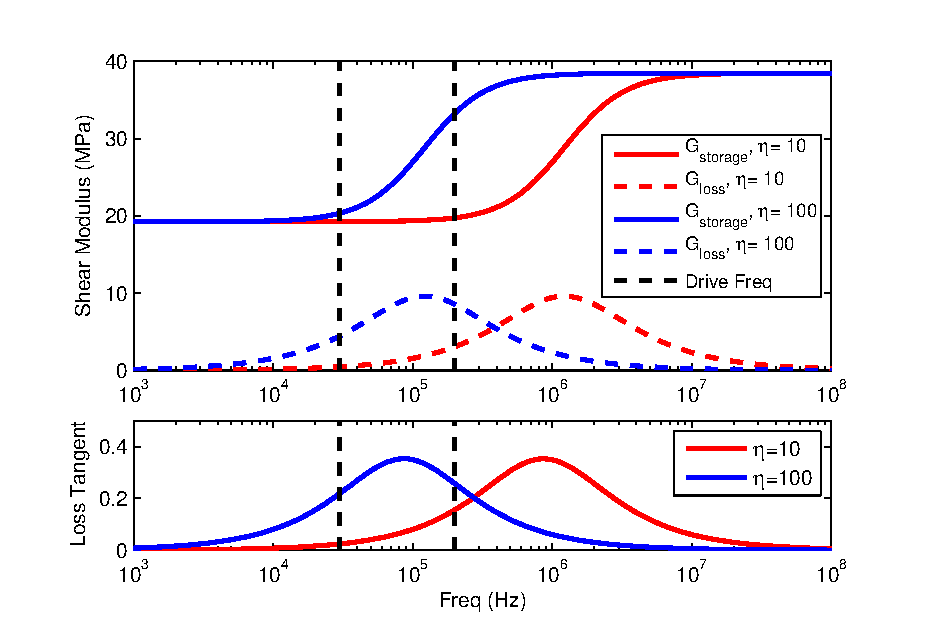
\includegraphics[width=4.5in]{scanbasic_ex2_dynamic_modulus} \caption{Dynamic Storage and Loss modulus for the two materials used in this
example. (\textbf{AMS} Example 2)}
\par\end{centering}
\centering{}\label{fig:AMS_ex2_dyn_mod} 
\end{figure}

\begin{figure}
\includegraphics{ams_ex2_sample_sch}
\begin{centering}
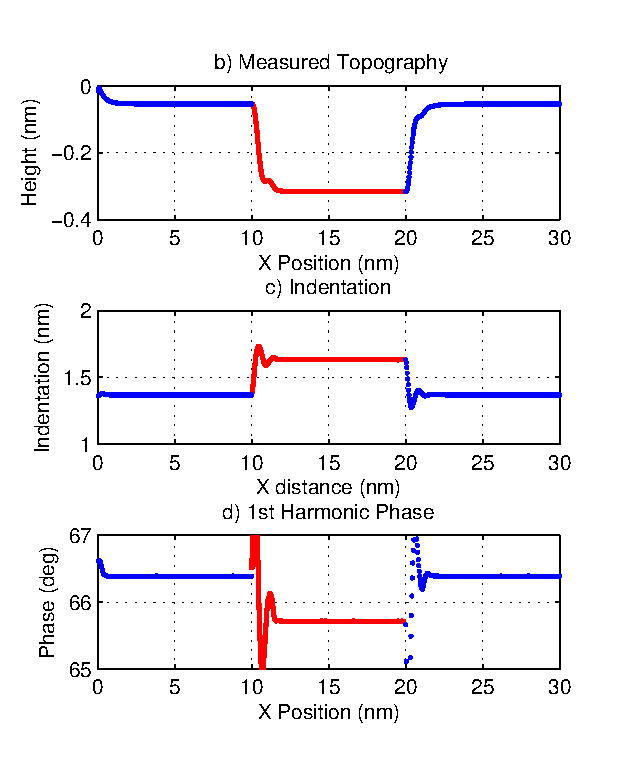
\includegraphics[clip,width=4.5in]{AMS_Ex2_H_P} \caption{a) Schematic of sample. There is a region in the middle (the ``feature'')
that has the same height as the surrounding area (the ``substrate'')
but different material properties. b) Measured topography vs. X distance
over which the AFM scans. The sample is actually flat so the step
in topography is an artifact. c) The indentation, which shows that
the measurement error is due to an increased indentation on the softer
region. d) The lock-in phase (deg) vs. X distance (nm). (\textbf{AMS}
Example 2)}
\par\end{centering}
\centering{}\label{fig:AMS_Ex2_H_P} 
\end{figure}

\begin{figure}[htb]
\begin{centering}
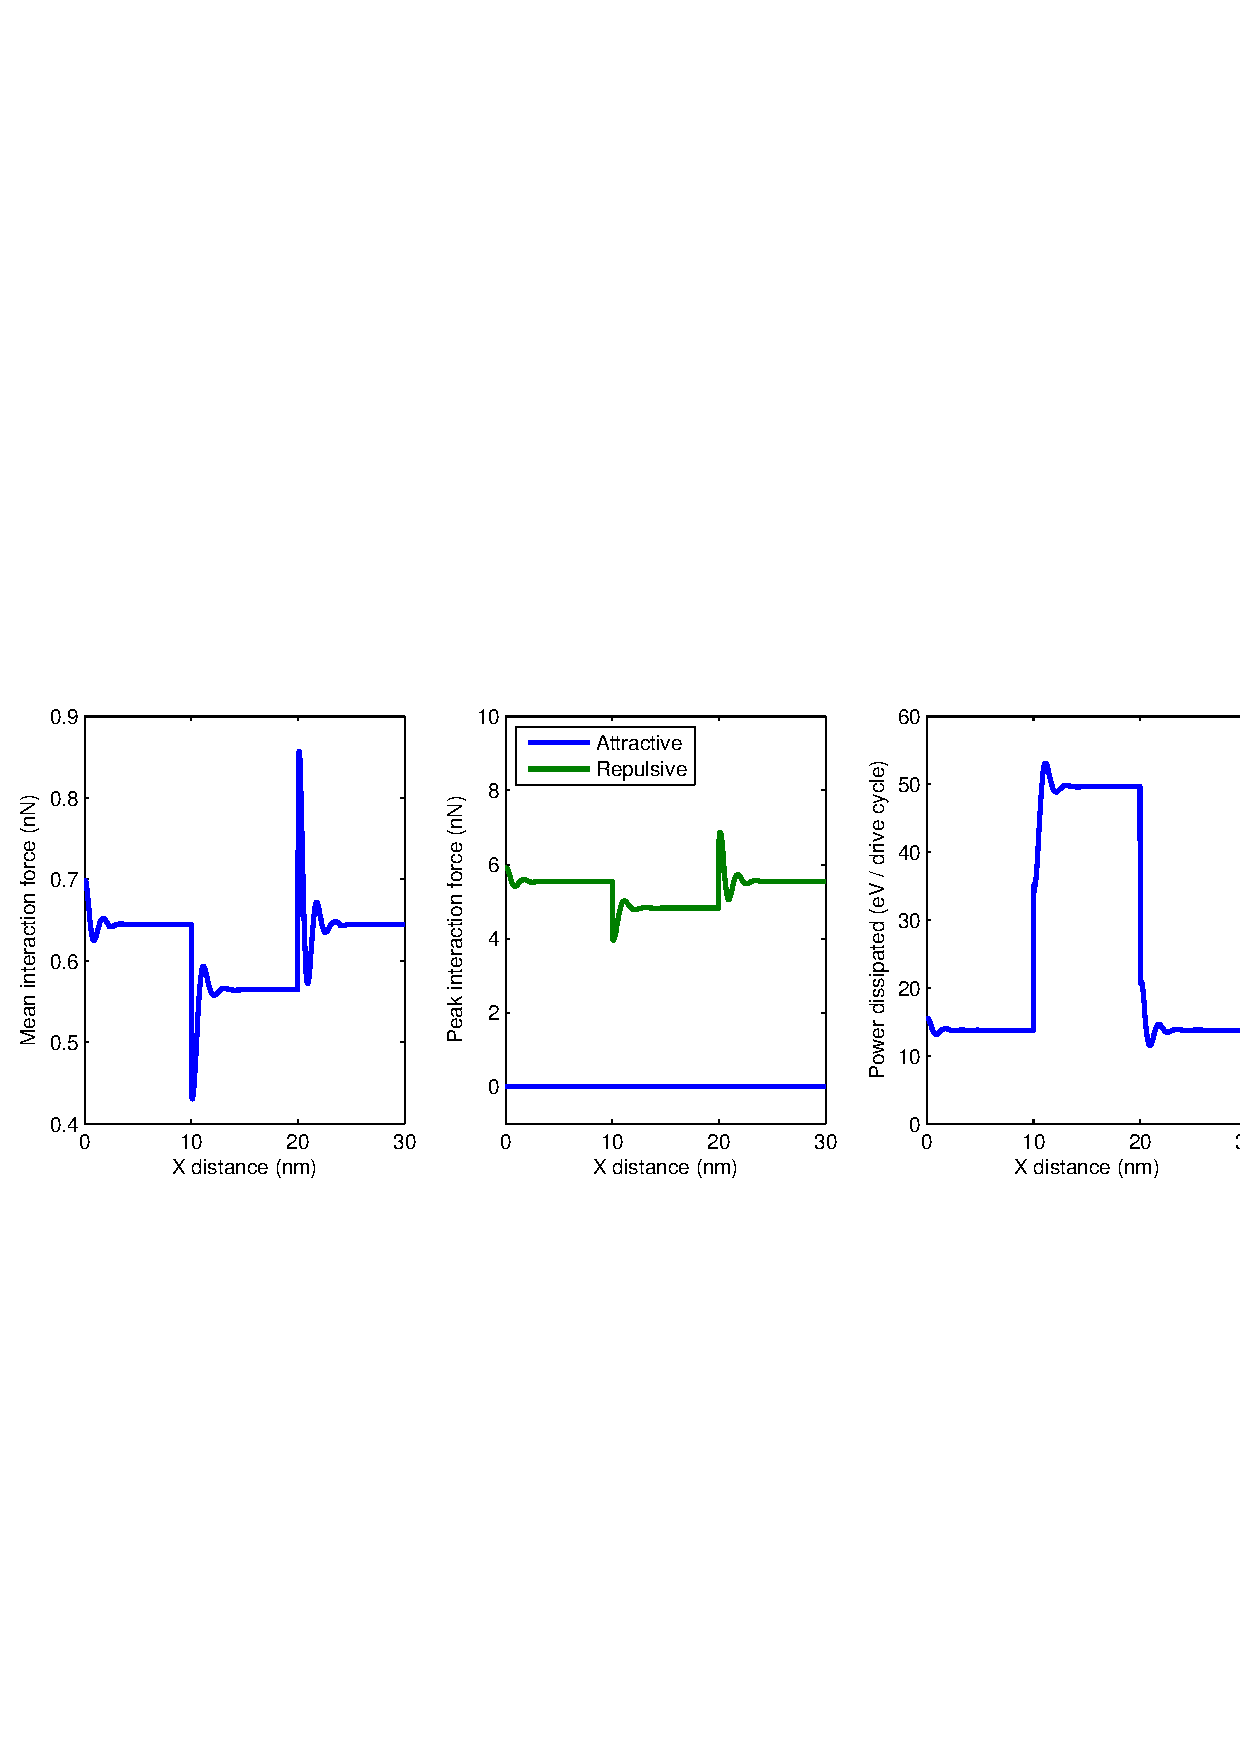
\includegraphics[width=5.5in]{AMS_Ex2_Mf_Pf_Wdot} \caption{(a) The mean interaction force (nN) vs. X distance (nm). The magnitude
of the average force is affected by the viscoelastic sample damping.
(b) Peak attractive and repulsive interaction forces (nN) vs. X distance.
(c) The tip-sample energy dissipation (eV / drive cycle) vs. X distance
(nm). (\textbf{AMS} Example 2)}
\par\end{centering}
\centering{}\label{fig:AMS_Ex2_Mf_Pf_Wdot} 
\end{figure}

\begin{figure}[htb]
\centering{}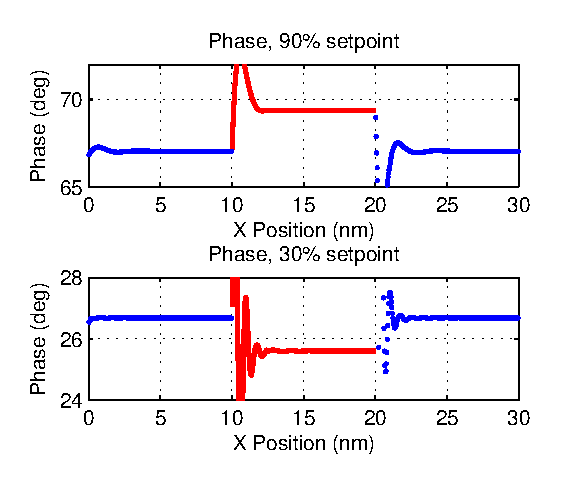
\includegraphics[clip,width=4.5in]{AMS_Ex2_higherfreq}
\caption{1st harmonic phase versus X for two different setpoints when the natural
frequency is increased to 200 kHz and the stiffness is raised to 40
N/m. There is now a phase contrast reversal between the different
setpoints.\label{fig:AMS_Ex2_higherfreq}}
\end{figure}

\begin{figure}

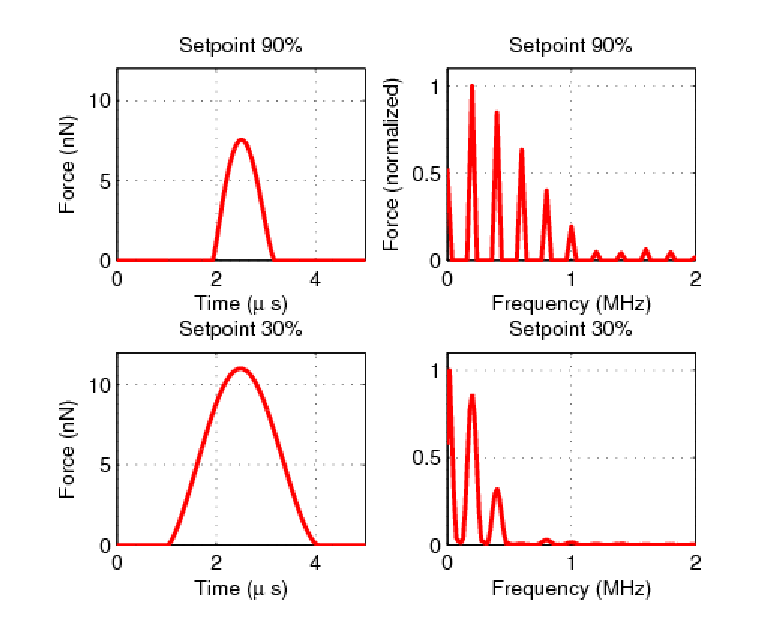
\includegraphics{AMS_Ex2_timehist}

\caption{\label{fig:AMS_Ex2_timehist}Time histories of force for the two different
setpoints in Figure \ref{fig:AMS_Ex2_higherfreq}. Also shown in the
Fourier transform of the time history. At the higher setpoint, the
contact time is shorter, which means higher frequency components.
At the lower setpoint, the contact time is longer, which means not
as many high frequency components. (\textbf{AMS Example 2})}

\end{figure}

\clearpage{}

\subsubsection{\label{sec:Tools.AMS.Ex3}Example 3: Effects of adhesion, Jumps between
regimes}

In the previous example, the topography error was largely attributed
to a difference in indentation caused by a difference in sample elasticity.
In this example we demonstrate that even for samples with identical
elasticity, there can be topography errors that are not related indentation.
This simulation consists of a hard substrate with a small step feature
on it. The feature has identical tip-sample interaction properties
to the substrate except that the Hamaker constant is slightly smaller.
We also explore consequences of the attractive and repulsive regimes
introduced in the Amplitude Modulated Approach Curves section. You
may wish to work through AMAC example 1 and 2 before trying this example.

You can run the example by choosing ``Example 3'' from the drop
down menu, or by entering the parameters from the table manually.
After the simulation runs look at the measured topography, Figure
\ref{fig:AMS_Ex3_topo1}. You will note that the red line indicates
the true topography and the blue line the measured topography. Clearly
there is a significant error.

It will be instructive in sorting this out to consider what really
is the effect on tip-sample interaction of changing the Hamaker constant
while keeping the intermolecular distance the same? The Force Viewer
tool can easily show this. This tool is explained in section \ref{sec:Tools.ForceViewer}.
For now, we simply present the result in figure \ref{fig:AMS_Ex3_Fts}.
We note that for the larger Hamaker constant, the minimum value of
force is smaller, although it occurs at the same gap. Also, for a
given force that is less than the minimum, say -1 nN, it occurs farther
from the sample surface with a larger Hamaker constant. Since tapping
mode images at a constant amplitude reduction, and to a rough approximation
the same amplitude reduction will happen with a similar force level,
we see that we might expect that with a larger Hamaker constant, the
cantilever will be farther away from the same surface at the same
amplitude reduction.

Now, is there anything that we could do to get a better scan? Examine
the mean interaction forces, shown in figure \ref{fig:AMS_Ex3_mf1}.
Note that they are negative for the whole scan. That is, we are imaging
in an attractive regime. We may guess that if we were to image in
an repulsive regime, the effects of the attractive forces may be less
important. The proper way to find the repulsive regime would be use
the Amplitude Modulated Approach Curves tool (section \ref{sec:Tools.DAC}).
For now, assume that we'll try to guess a better set of parameters.
Lower the setpoint ratio from 0.98 to 0.95 and re-run the simulation.
The results should look like Figure \ref{fig:AMS_Ex3_topo2}. This
is actually worse than before. Not only is the feature height incorrect,
the section of substrate after the feature is incorrect as well. What
is going on here? Again, examine the mean interaction forces for a
clue, see Figure \ref{fig:AMS_Ex3_mf2}. Note that the substrate section
at the begining of the scan has an repulsive mean force while the
substrate section at the end of the scan has an attractive mean force.
We are now in a bi-stable region, which is even worse.

Again, the proper way to correct this situation is to perform Amplitude
Modulated Approach Curves and find a good region for imaging. For
now, try the following: raise the Unconstrained Amplitude from 13
nm to 25 nm. The results show now like look figures \ref{fig:AMS_Ex3_topo3}
and \ref{fig:AMS_Ex3_mf3}. The topography error is now much smaller
on the step, and the mean interaction forces are repulsive for the
whole scan. You'll note, of course, that now we have some overshoot
at the leading edge of the step. This is due to poor controller gains.
We briefly discussed controller gains in the next example.

\begin{figure}[htb]
\begin{centering}
\includegraphics[clip,width=4.5in]{AMS_Ex3_topo1} \caption{Measured topography and sample height. (\textbf{AMS} Example 3)}
\par\end{centering}
\centering{}\label{fig:AMS_Ex3_topo1} 
\end{figure}

\begin{figure}[htb]
\begin{centering}
\includegraphics[clip,width=4.5in]{AMS_Ex3_Fts} \caption{Tip-sample interaction forces for (\textbf{AMS} Example 3). The bold
line is A=3.4e-20, the thin line is A=6.8e-20}
\par\end{centering}
\centering{}\label{fig:AMS_Ex3_Fts} 
\end{figure}

\begin{figure}[htb]
\begin{centering}
\includegraphics[clip,width=4.5in]{AMS_Ex3_mf1} \caption{Mean interaction forces. (\textbf{AMS} Example 3)}
\par\end{centering}
\centering{}\label{fig:AMS_Ex3_mf1} 
\end{figure}

\begin{figure}[htb]
\begin{centering}
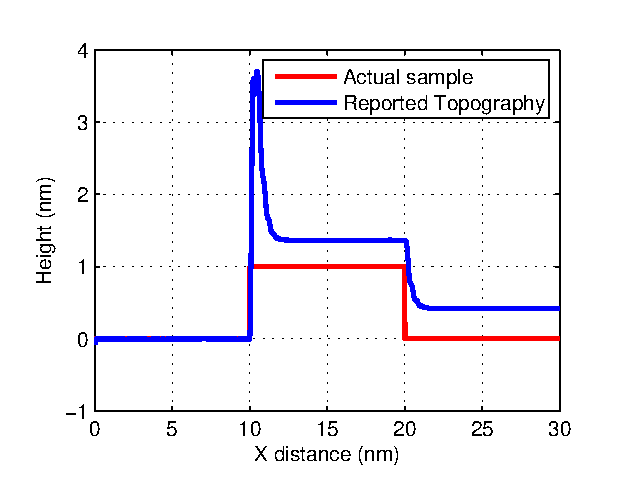
\includegraphics[clip,width=4.5in]{AMS_Ex3_topo2} \caption{Measured topography and sample height, with setpoint lowered to 0.65
(\textbf{AMS} Example 3)}
\par\end{centering}
\centering{}\label{fig:AMS_Ex3_topo2} 
\end{figure}

\begin{figure}[htb]
\begin{centering}
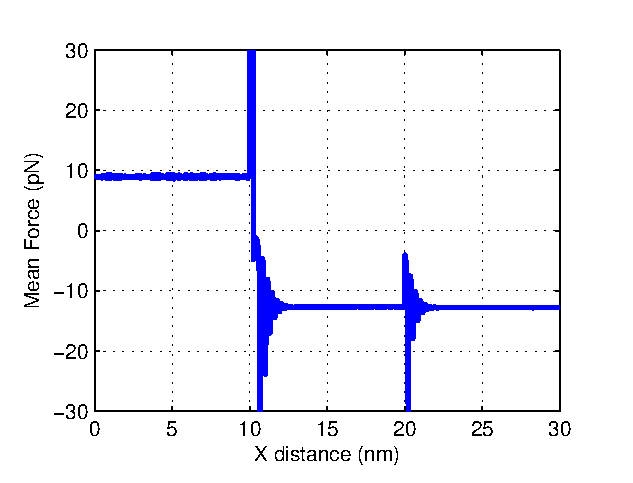
\includegraphics[clip,width=4.5in]{AMS_Ex3_mf2} \caption{Mean interaction forces with setpoint lowered to 0.65 (\textbf{AMS}
Example 3)}
\par\end{centering}
\centering{}\label{fig:AMS_Ex3_mf2} 
\end{figure}

\begin{figure}[htb]
\begin{centering}
\includegraphics[clip,width=4.5in]{AMS_Ex3_topo3} \caption{Measured topography and sample height with unconstrained amplitude
raised to 25 nm. (\textbf{AMS} Example 3)}
\par\end{centering}
\centering{}\label{fig:AMS_Ex3_topo3} 
\end{figure}

\begin{figure}[htb]
\begin{centering}
\includegraphics[clip,width=4.5in]{AMS_Ex3_mf3} \caption{Mean interaction forces with unconstrained amplitude raised to 25
nm. (\textbf{AMS} Example 3)}
\par\end{centering}
\centering{}\label{fig:AMS_Ex3_mf3} 
\end{figure}

\clearpage{}



\subsubsection{\label{sec:Tools.AMS.Ex4}Example 4: Effect of controller gains}


In this section we explore the effects of controller gains on the
scanning response. There are many factors which affect the response,
the largest ones are scanning speed (slower speed = more accurate
scan), setpoint ratio, lock-in time constants, and controller gains.
In this example we will explore only the controller integral gains.

This example use the same basic parameters from Example 3 but the
feature material properties to be the same as the substrate. To run
this example, first select Example 4 from the Example loader drop
down menu. The initial value of Integral gain will be 0.001. Run this
simulation. Then click Input to go back, and enter an integral of
0.002. Repeat for 0.004 and 0.008. Then, examine the topography response
(click the All button to overlay the results). If you zoom in, it
should look similar to Figure \ref{fig:AMS_Ex4}, your lines may be
different colors. The blue line in this example corresponds to a gain
of 0.001. This gain is clearly a little low, it takes awhile for the
controller to respond when it hits the step edge. The green line is
0.002. This is a little better. The purple line is 0.004. This response
is much quicker, but now there is some overshoot. Finally, the orange
line is 0.008. This gain is so high that the controller is on the
verge of going unstable, and rings significantly.

If we take this example to the extreme, try entering an integral gain
of 0.032. You will note that the transient percent number fluctuates
rapidly and does not converge. Eventually, it will give up without
ever performing the simulation. This represents the fact that the
controller cannot stabilize on the substrate surface and so it cannot
even begin the scan (let alone the step edge). You will note that
are some hints on stabilizing the controller in the ``ErrorMessage''
drop down. Conversely, if we enter a value of 0.00001 for the integral
gain, the controller will take so long to stabilize on the substrate
surface that it will time out.

\begin{figure}[htb]
\begin{centering}
\includegraphics[clip,width=4.5in]{AMS_Ex4} \caption{The effect of integral gain on the measured topography response. (\textbf{AMS}
Example 4)}
\par\end{centering}
\centering{}\label{fig:AMS_Ex4} 
\end{figure}



\subsubsection{\label{sec:Tools.AMS.Ex5}Example 5: Controller Instability}


 In this example we demonstrate an imaging artifact that can occur
on sticky (i.e. highly adhesive) samples. Choose example 5 from the
Example loader. Note that this simulation models the substrate with
Hertz contact (no adhesion) and the feature with DMT contact (adhesion).
When you run the simulation, the measured topography should look like
Figure \ref{fig:AMS_Ex5_1}. On the feature (between X=25 and X=75),
there is a series of sharp spikes. The cantilever appears to be jumping
away from the surface for some reason. This is apparently some kind
of controller instability. Based on the results in the previous example,
we might try to decrease the controller gains. However that will not
change the behavior (try it for yourself).

The best way to determine what is going on is to open the Dynamic
Approach Curves tool and examine the approach curve for the cantilever
and sample parameters. In particular, we should examine the behavior
around 70\% setpoint ratio that we are using in this example. Perform
one run for the substrate (Hertz contact) and one for the sample (DMT).
The result should look like \ref{fig:AMS_Ex5_2}. On the substrate
(red curve) the amplitude is reduced smoothly to zero as the cantilever
approaches the surface. But on the sample, the cantilever snaps in
to permanent contact with the surface at about A=4.5 nm (75\% setpoint).

We can now explain the scanning behavior. The cantilever starts far
from the surface with a large amplitude. The controller brings the
cantilever closer to the surface to reduce the amplitude. However,
before the amplitude is reduced to the setpoint of 70\%, the cantilever
snaps-in and the amplitude jumps to nearly 0. The controller sees
that this amplitude reduction has gone too far, and pulls the cantilever
away from the sample in order to increase the amplitude. The process
then repeats.

There simply is no settings of controller gains or scannin speeds
that would make this system stable. In a real experiment, the only
two choice would be to raise the setpoint ratio to a point that is
stable (e.g. 80\%), or to change the free amplitude. Raising the setpoint
is simple enough, but the behavior on change the free amplitude may
be non-intuitive. Try raising the unconstrained amplitude to 7 nm,
and then decreasing it to 5 nm. Which one gives a larger stable region
(in terms of amplitude ratio)?

You should find that raising the free amplitude decreases the width
of the stable region (i.e. the jump happens at 80\% instead of 75)
but lowering the free amplitude increases the width of the stable
region (i.e. the jump happens at 70\% instead of 75). Why should this
be? The answer has to do with the stability of dynamic systems, and
is somewhat out of the scope of this manual. The curious reader is
encouraged to find an introductory text on mechanical vibrations.

\begin{figure}[htb]
\begin{centering}
\includegraphics[clip,width=4.5in]{AMS_Ex5_1} \caption{Measured topography. The large spikes represent a controller instability.
(\textbf{AMS} Example 5)}
\par\end{centering}
\centering{}\label{fig:AMS_Ex5_1} 
\end{figure}

\begin{figure}[htb]
\begin{centering}
\includegraphics[clip,width=4.5in]{AMS_Ex5_2} \caption{Approach curves on the substrate (red) and sample (blue). On the sample,
the cantilever snaps in to the surface due to the large attractive
forces. (\textbf{AMS} Example 5)}
\par\end{centering}
\centering{}\label{fig:AMS_Ex5_2} 
\end{figure}

\newpage{}



\subsection{\label{sec:Tools.DAC Advanced}Amplitude Modulated Approach Curves:
Advanced}


Microcantilevers are used to image biological and other materials
in liquids. The Amplitude Modulated Approach Curves: Advanced (\textbf{AMAC:
Advanced}) tool was originally developed to simulate the response
of an excited microcantilever approaching a sample in liquid; however,
it can also be used for multi-mode simulations in air or vacuum. Both
the first and second flexural eigenmodes of the cantilever are considered
in the simulation (this allows for a better approximation of the cantilever
response in liquid).

The following assumptions are made in the \textbf{AMAC Advanced} tool: 
\begin{enumerate}
\item Cantilever dynamics are modeled by the multiple eigenmode model (Eq.
\ref{eq:ndmdof}). 
\item Interactions between the tip and the sample are modeled by any one
of the models described in Section \ref{sec:fts}. 
\item The cantilever is either acoustically excited or magnetically excited
\cite{Xu_JAP_2007}. 
\item The cantilever excitation occurs through either a single frequency
(conventional) or two-frequencies (bimodal). 
\item The $Z$ separation between the sample can be reduced or increased,
but the cantilever does not move laterally. Inertial and hydrodynamic
forces caused by the $Z$ motion are negligible. 
\end{enumerate}
This section provides an overview of the outputs of the AMAC: Advanced
tool in the form of several example simulations. 
\begin{table}[H]
\caption{\label{tab:ADACEx}Input parameters for AMAC: Advanced examples.}

\begin{ruledtabular} %
\begin{tabular}{lrrrrr}
~~~~\textbf{PARAMETER} & \textbf{EX. 1} & \textbf{EX. 2} & \textbf{EX. 3} & \textbf{EX. 4} & \textbf{EX. 5}\tabularnewline
~ &  &  &  &  & \tabularnewline
\textbf{Operating conditions, cantilever properties} &  &  &  &  & \tabularnewline
~~~~Choose excitation source & Magnetic & Magnetic & Magnetic & Magnetic & Acoustic\tabularnewline
~~~~Choose frequency scheme & Single freq. & Two freq. & Single freq. & Two freq. & Two freq.\tabularnewline
~~~~Number of eigenmodes  & 2 & 2 & 2 & 2 & 2\tabularnewline
~~~~Unconstrained Amplitude (nm) & 10 & 10 & 20 & 20 & 17\tabularnewline
~~~~Unconstrained Amplitude (2nd drive frq) (nm) & NA & 1 & NA & 1.17 & 0.56\tabularnewline
~~~~Auto calculate $k_{i}~(i>1)$? & no & no & no & no & yes\tabularnewline
~~~~$k_{i}$ (N/m) & 0.036, 1.4 & 0.036, 1.4 & 30, 1200 & 30, 1200 & 0.9\tabularnewline
~~~~$Q_{i}$ & 1.2, 2 & 1.2, 2 & 400, 1200 & 400, 1200 & 225, 1000\tabularnewline
~~~~$f_{i}$ (kHz) & 9.3, 72 & 9.3, 72 & 350, 2450 & 350, 2275 & 48.9, 306.6\tabularnewline
~~~~$f_{d}$ (kHz) & 9.3 & 9.3,72 & 350 & 350,2275 & 48.9, 306.6\tabularnewline
~~~~Tip mass, ($m_{tip}/m_{c}$) & 0 & 0 & 0 & 0 & 0\tabularnewline
~~~~Z approach velocity (nm/s) & 20 & 20 & 100 & 100 & 100\tabularnewline
~~~~Z range Determination & Autocalc & Autocalc & Autocalc & Autocalc & Specify\tabularnewline
~~~~Lock-in Time Constant (us) & 500 & 500 & NA & NA & 200\tabularnewline
~ &  &  &  &  & \tabularnewline
\textbf{Tip-sample interaction properties} &  &  &  &  & \tabularnewline
~~~~Tip-sample interaction model & Hertz & Hertz & Hertz & Hertz & DMT\tabularnewline
~~~~Tip radius (nm) & 30 & 30 & 10 & 10 & 20\tabularnewline
~~~~Young's modulus of tip (GPa) & 130 & 130 & 130 & 130 & 130\tabularnewline
~~~~Poisson's ratio of the tip & 0.3 & 0.3 & 0.3 & 0.3 & 0.3\tabularnewline
~~~~Intermolecular Distance & NA & NA & NA & NA & 0.1\tabularnewline
~~~~Hamaker constant & NA & NA & NA & NA & 4e-20\tabularnewline
~~~~Young's modulus of sample (GPa) & 10 & 1 & 1, 5 & 1, 5 & 1e-6\tabularnewline
~~~~Poisson's ratio of the sample & 0.3 & 0.3 & 0.3 & 0.3 & 0.3\tabularnewline
~~~~Include visco-elastic forces? & none & Kelvin-voigt & none & none & none\tabularnewline
~~~~Sample viscosity (Pa$\cdot$ s) & NA & 100 & NA & NA & NA\tabularnewline
~ &  &  &  &  & \tabularnewline
\textbf{Simulation parameters} &  &  &  &  & \tabularnewline
~~~~Number of points plotted & 1000 & 750 & 500 & 500 & 1000\tabularnewline
~~~~Deflection points per cycle & 1000 & 1000 & 1000 & 1000 & 1000\tabularnewline
~~~~Plot a higher harmonic? & no & no & yes & no & no\tabularnewline
~~~~Number of higher harmonics & NA & NA & 1 & NA & NA\tabularnewline
~~~~Choose higher harmonics & NA & NA & 7 & NA & NA\tabularnewline
~~~~Include time histories & yes & yes & yes & yes & no\tabularnewline
~~~~Number of time histories & 3 & 1 & 1 & 1 & NA\tabularnewline
~~~~Choose amplitude ratio(s) & 0.95, 0.9, 0.5 & 0.9 & 0.9 & 0.9 & NA\tabularnewline
~~~~Number of cycles & 2 & 2 & 2 & 4 & NA\tabularnewline
~~~~Choose X-axis variable & Amp. ratio & Z-distance & Amp. ratio & Amp. ratio & Amp. ratio\tabularnewline
\end{tabular}\end{ruledtabular} 
\end{table}

\newpage{}



\subsubsection{\label{sec:Tools.DAC Advanced.Ex1}Example 1: Multiple impact regimes
for a Biolever in liquid}


In this example, we will simulate a Biolever approaching a mica sample
in a buffer solution and observe oscillations with multiple impacts
per oscillation period \cite{Melcher_APL_2008}. We will show how
abrupt transitions in the phase correspond to grazing trajectories
which indicate multiple impact oscillations. Refer to Table \ref{tab:ADACEx},
Example 1 for the correct input values.

To begin this example, open the \textbf{Amplitude Modulated Approach
Curves (Advanced)} tool from the \textbf{VEDA} tools selection. Wait
for the user input window to open (you should start in the \emph{Operating
conditions and cantilever properties} tab). Either select ``Example
1'' from the \emph{Example Loader} dropdown box, or follow these
instructions to set the parameters manually: Change the \emph{excitation
source} to \emph{Magnetic}. Enter the first and second natural frequencies
in \emph{f (kHz)} and excitation frequencies both as comma delimited
values: $9.3,~72$. Next, click on the \emph{Tip-sample interaction
properties} tab. Verify the \emph{Include sample viscoelastic forces}
is set to \emph{None}, and change the \emph{Young's modulus of sample
(GPa)} to 10. Now, click on the \emph{Simulation parameters} tab.
Check the \emph{Include sample of time histories} box. Make sure that
the \emph{Number of time histories to collect} is 3, and that the
corresponding amplitude ratios are 0.95, 0.9, 0.5. Set the \emph{Number
of cycles included in sample} to 2. Finally, click \emph{Simulate}
and wait for the simulation to reach completion. The simulation runs
in less than one minute.

The simulation records three extractions of deflection/tip-sample
interaction time histories. The first corresponds to an amplitude
ratio $A_{1}/A_{0}=0.95$ (see Figure \ref{fig:ADACex1_D_TS}a). At
this amplitude ratio, single impact oscillations are observed where
the tip makes contact with the sample once per oscillation period.
Closer to the sample, at an amplitude ratio $A_{1}/A_{0}=0.9$ (see
\ref{fig:ADACex1_D_TS}b), double impact oscillations are observed
and eventually triple impacts occur are found at $A_{1}/A_{0}=0.5$
(see Figure \ref{fig:ADACex1_D_TS}c).

Looking at the phase of the response (Figure \ref{fig:ADACex1_P}),
we have identified the precise amplitude ratios where transitions
to the indicated multiple impact regime occurs where $Gn$ marks to
grazing trajectory which leads to an amplitude branch where $n$ impacts
per oscillation occur. Not surprisingly, we can see in Figure \ref{fig:ADACex1_Mf_Pf}
and Figure \ref{fig:ADACex1_C} that characteristics of the interaction
with the sample (mean force, peak force) are affected by multiple
impact regimes.

\begin{figure}[htb]
\begin{centering}
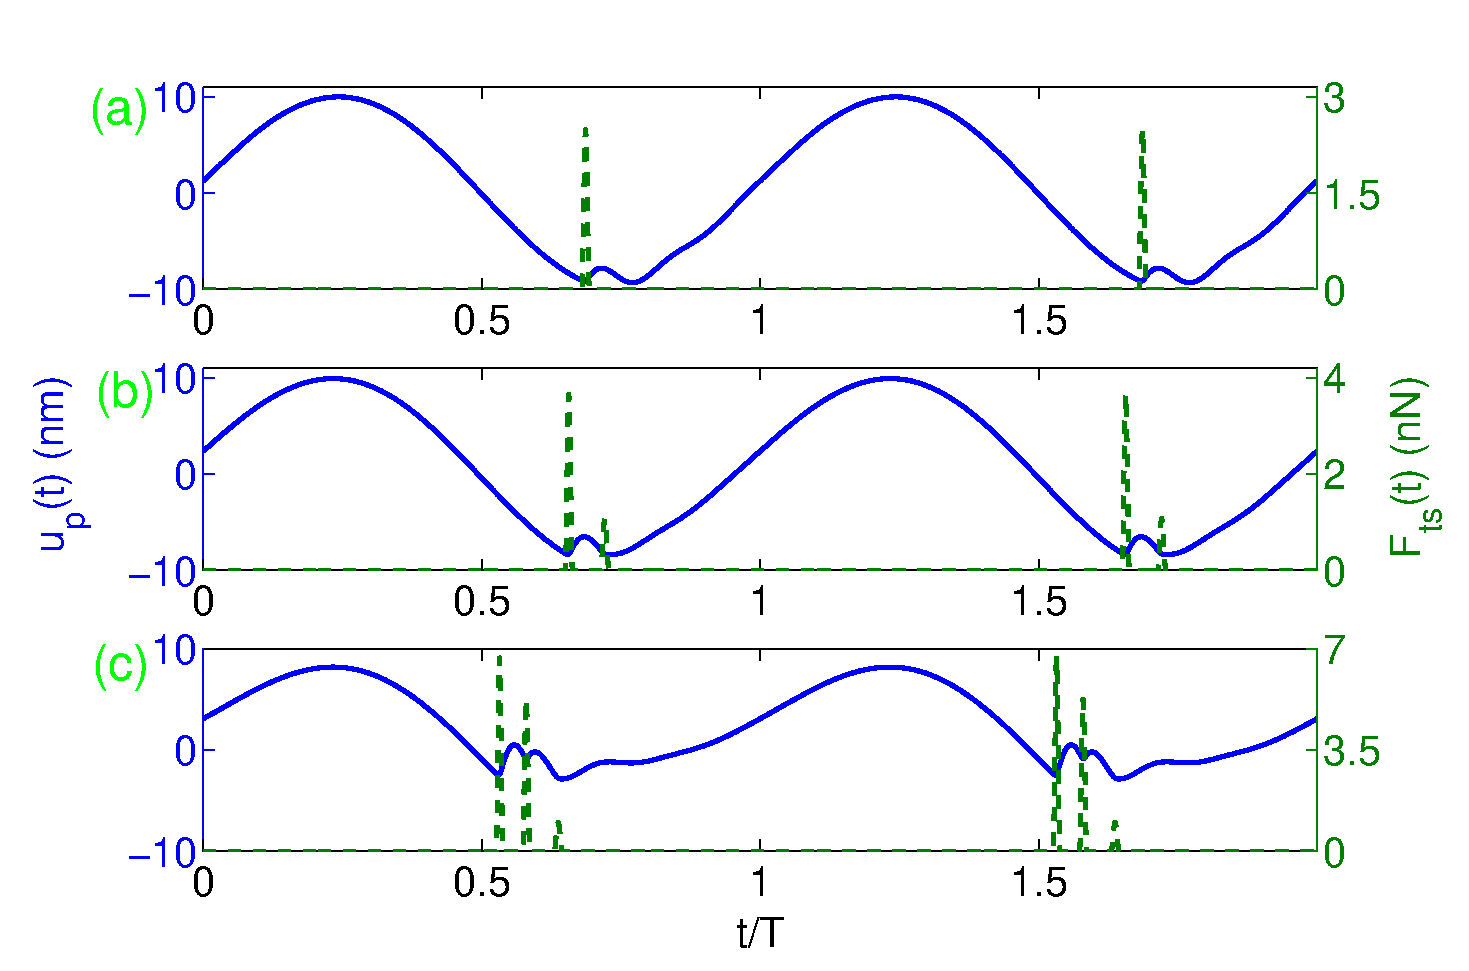
\includegraphics[width=3.5in]{ADACex1_D_TS} \caption{Photodiode deflection signal $u_{p}(t)$ and tip-sample interaction
force $F_{ts}(t)$ fro two periods of oscillation at amplitude ratios
$A_{1}/A_{0}$ of 0.95 (a), 0.9 (b), and 0.5 (c). Each time the cantilever
passes a grazing point, an additional impact with the sample is added
to the oscillation cycle. (\textbf{AMAC Advanced} Example 1)}
\par\end{centering}
\centering{}\label{fig:ADACex1_D_TS} 
\end{figure}

\begin{figure}[htb]
\begin{centering}
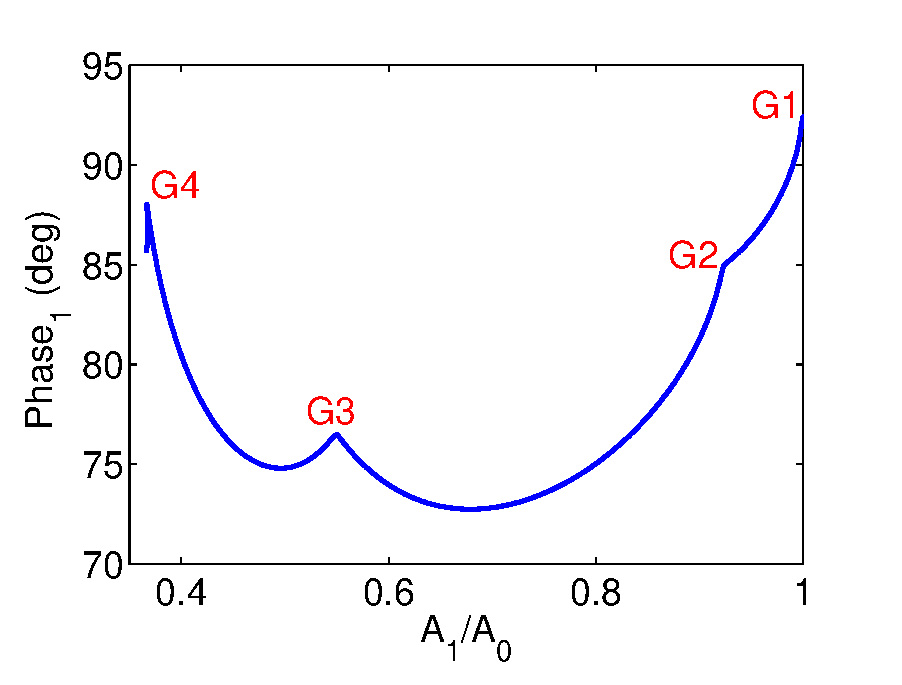
\includegraphics[width=3.5in]{ADACex1_P} \caption{Phase (deg) of the primary harmonic vs. amplitude ratio $A_{1}/A_{0}$.
G1-G4 are grazing points where the cantilever tip contacts the sample
at zero velocity (\textbf{AMAC Advanced} Example 1).}
\par\end{centering}
\centering{}\label{fig:ADACex1_P} 
\end{figure}

Figure \ref{fig:ADACex1_C} demonstrates that tip-sample contact time
for soft cantilevers in liquids behaves much differently than stiff
cantilevers in air (see Figure \ref{fig:DACex2_C}). Inside a given
impact regime, contact time is actually decreasing as amplitude ratio
decreases. This is happens because of the role momentary excitation
of the second eigenmode during tip-sample contact. Secondly, we see
that contact time increases nearly stepwise near the beginning of
a multiple impact regime, also indicating the importance of second
eigenmode dynamics to tip-sample contact for soft cantilevers in liquids.

\begin{figure}[htb]
\begin{centering}
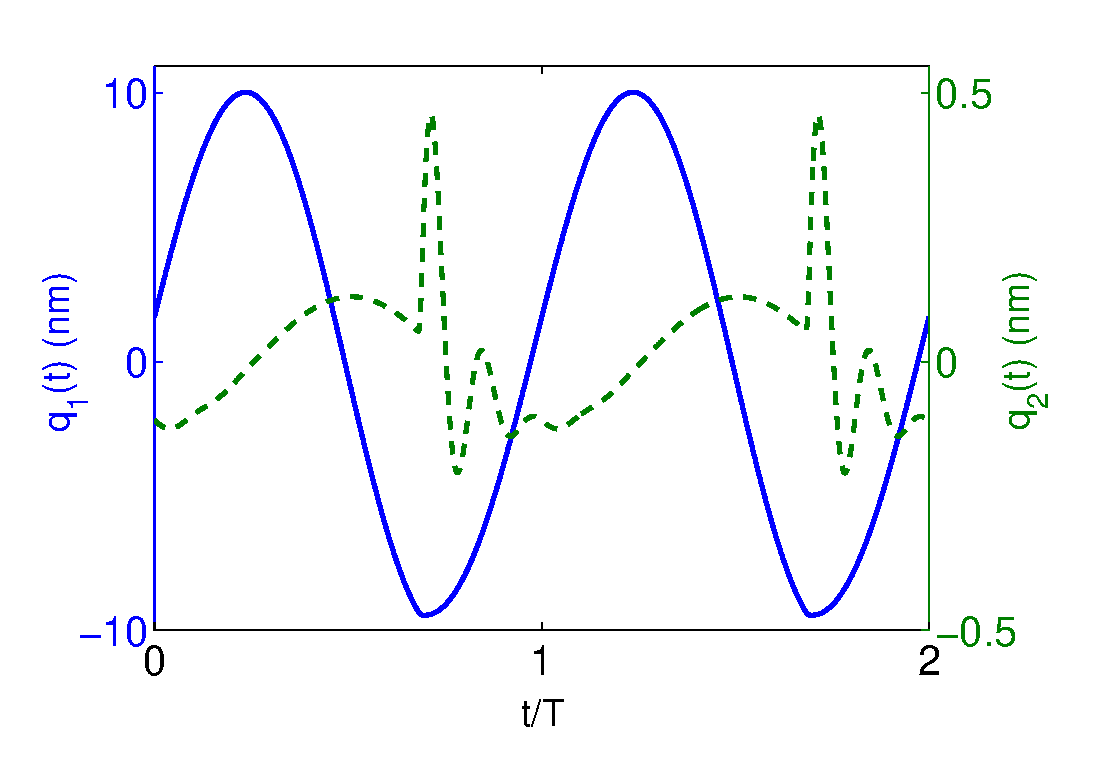
\includegraphics[width=3.5in]{ADACex1_Eig} \caption{Response of the first $q_{1}(t)$ and second $q_{2}(t)$ eigenmodes
tapping at an amplitude ratio $A_{1}/A_{0}=0.95$. Near times of contact
with the sample, the second eigenmode becomes momentary excited and
then decays. A slower varying deflection is caused by the excitation
force. (\textbf{AMAC Advanced} Example 1)}
\par\end{centering}
\centering{}\label{fig:ADACex1_Eig} 
\end{figure}

\begin{figure}[htb]
\begin{centering}
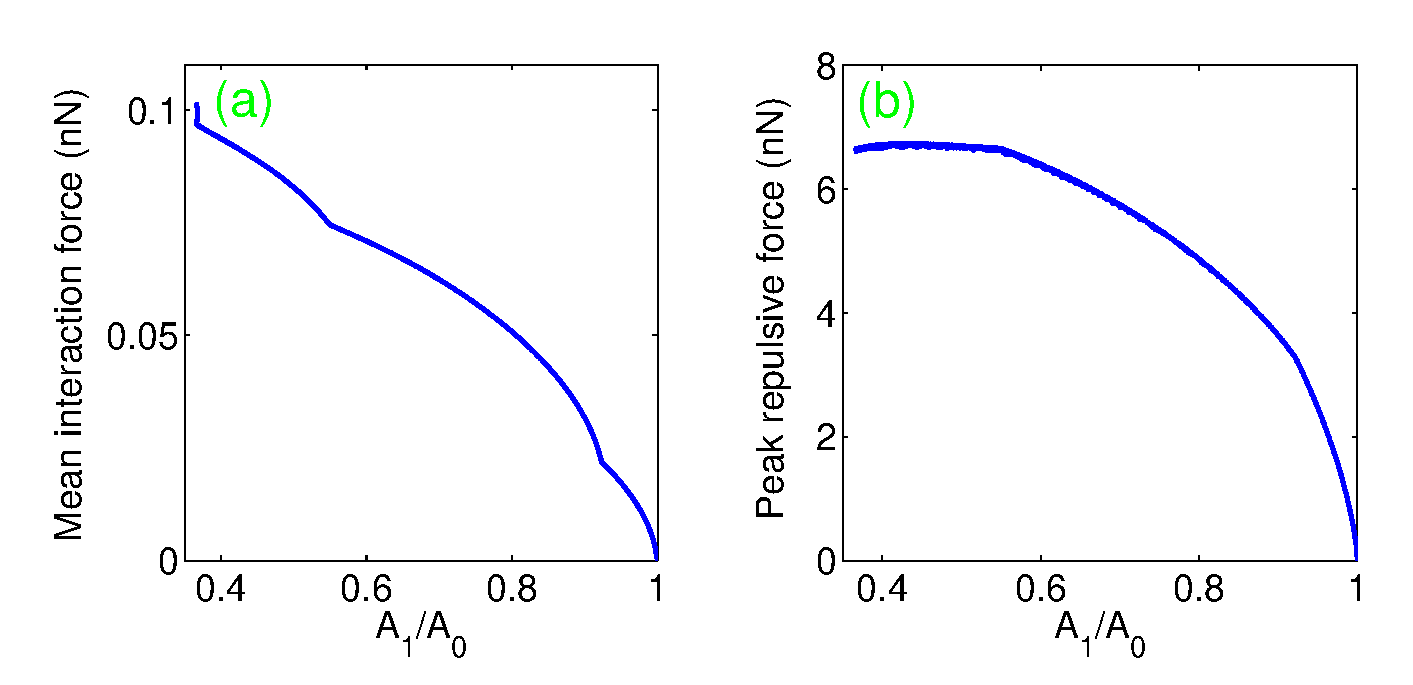
\includegraphics[width=5in]{ADACex1_Mf_Pf} \caption{Mean (a) and peak repulsive (b) interaction forces (nN) vs. amplitude
ratio. A sharp change in their trends occurs near the grazing trajectories.
(\textbf{AMAC Advanced} Example 1)}
\par\end{centering}
\centering{}\label{fig:ADACex1_Mf_Pf} 
\end{figure}

\begin{figure}[htb]
\begin{centering}
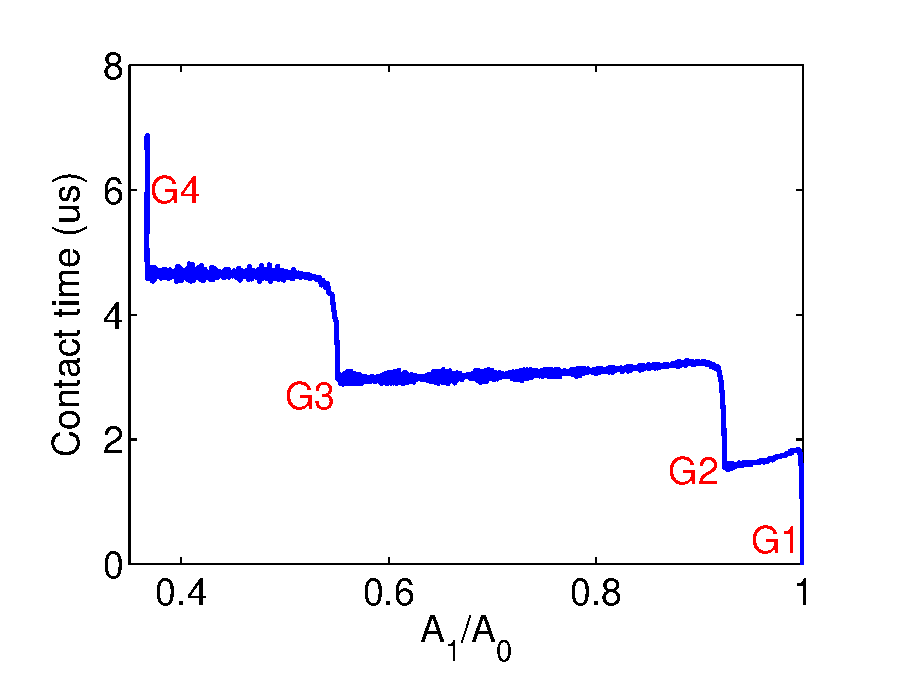
\includegraphics[width=3.5in]{ADACex1_C} \caption{Contact time ($\mu s$) vs. amplitude ratio $A_{1}/A_{0}$. Notice
the abrupt change in contact time occurring near each grazing point.
(\textbf{AMAC Advanced} Example 1)}
\par\end{centering}
\centering{}\label{fig:ADACex1_C} 
\end{figure}



\subsubsection{\label{sec:Tools.DAC Advanced.Ex2}Example 2: Bimodal excitation
of a Biolever in a liquid environment}


In this example, we will simulate a Biolever being excited at its
first two natural frequencies in a liquid environment. Refer to Table
\ref{tab:ADACEx}, Example 2 for the correct input values.

Because the least common multiple of two drive periods $\omega_{d1}=\omega_{1}=2\pi\cdot9.3$
kHz and $\omega_{d2}=\omega_{2}=2\pi\cdot72$ kHz is large, the period
of the overall oscillation is long $T=0.0033$s, which is very long
compared to the period of the fundamental drive. This requires a much
longer lock-in time constant for a good measurement. In this example,
we compare two lock-in time constants: of $500$ us and time constant
of $5$ ms.

To begin this example, open the \textbf{AMAC Advanced} tool from the
\textbf{VEDA} tools selection. Wait for the user input window to open
(you should start in the \emph{Operating conditions and cantilever
properties} tab). Either select ``Example 2'' from the \emph{Example
Loader} dropdown box, or follow these instructions to set the parameters
manually: Change the \emph{excitation source} to \emph{Magnetic} and
change the \emph{Frequency scheme} to \emph{two frequencies (bimodal)}.
Change the first and second natural frequencies in \emph{f (kHz)}
to $9.3,~72$, and include two drive frequencies \emph{$f_{d}$ (kHz)}
to 9.3,~72. Set \emph{Z approach velocity (nm/s)} to 20. Uncheck
the \emph{Autocalculate Time Constant} box and manually the set \emph{Lockin
Time constant} to 500 $\mu$s. Next, click on the \emph{Tip-sample
interaction properties} tab. Set the \emph{Young's modulus of sample
(GPa)} to 1. Under the \emph{Non-conservative forces} box, choose
\emph{Kelvin-voigt} for the \emph{sample viscoelastic forces} dropdown
box and set the \emph{Sample viscosity ($Pa\cdot s$)} to 100. Now,
click on the \emph{Simulation parameters} tab. Make sure the \emph{Include
sample of time histories} box is checked. Set the \emph{Number of
time histories to collect} to 1, and that the corresponding amplitude
ratio is 0.9 only. Set the \emph{Number of cycles included in sample}
to 2. Set the \emph{X-axis variable} to \emph{Z-distance (nm)} for
this example. At the bottom of this tab, uncheck \emph{Fourier} so
that only the lock-in computations are plotted not the Fourier integrals
(for clarity in the plots)

Finally, click the \emph{Simulate} button in the lower right-hand
corner, and wait for the simulation to reach completion. Once the
simulation has completed, click the \emph{Input} button. Open the
\emph{Operating conditions and cantilever properties} tab, and change
the \emph{Lock-in Time Constant} to 5 ms. Then, click the \emph{Simulate}
button again, and wait for the second simulation to reach completion.
For this example, each run generally takes less than 1 minute to complete.

The amplitudes of the primary and secondary excitations are shown
in Figure \ref{fig:ADACex2_AT} (a) and (b), respectively, for lock-in
time constants of 500 us and 5 ms. Only after increasing the lock-in
time constant by an order of magnitude does the amplitude of the second
eigenmode converge. The reason for this becomes clear looking at the
time history in Figure \ref{fig:ADACex2_DTS}. The second eigenmode
interacts sporadically with the sample due to the combination of external
forcing excitation and the momentary excitation from the tip-sample
interaction. This leads to mixture of single and double impact oscillations
occurring at the same amplitude ratio.

\begin{figure}[htb]
\begin{centering}
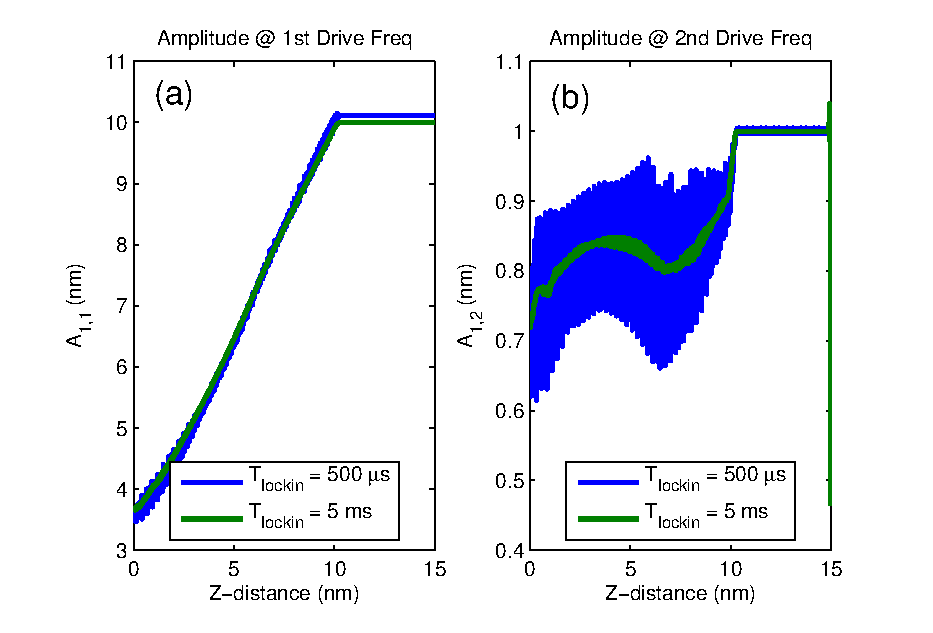
\includegraphics[width=5.5in]{ADACex2_AT} \caption{Amplitude (nm) vs. Z-distance (nm) for the first (\emph{Left}) and
second (\emph{Right}) frequencies. Two simulations were performed
with two different lock-in time constants: 500 us and 5 ms. (\textbf{AMAC
Advanced} Example 2)}
\par\end{centering}
\centering{}\label{fig:ADACex2_AT} 
\end{figure}

\begin{figure}[htb]
\begin{centering}
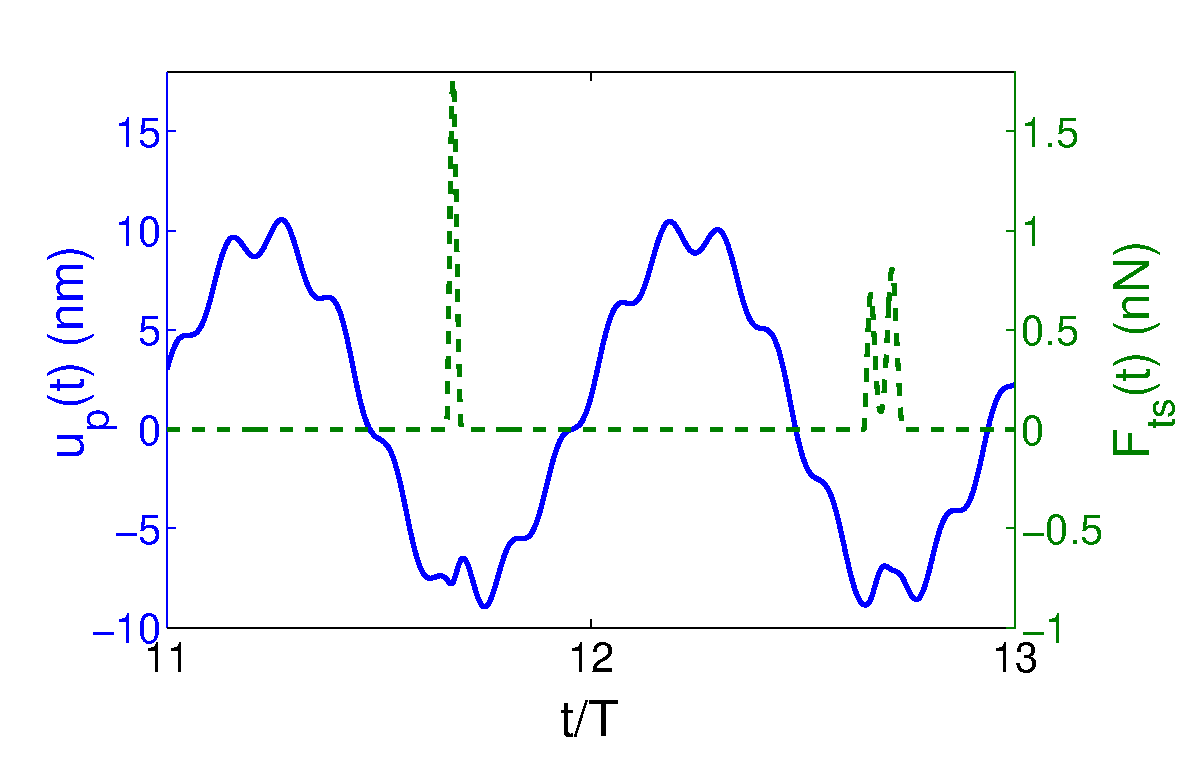
\includegraphics[width=3.5in]{ADACex2_DTS} \caption{Photodiode deflection signal $u_{p}(t)$ and tip-sample interaction
force vs. Z-distance (nm) at an amplitude ratio $A_{1}/A_{0}=0.9$.
(\textbf{AMAC Advanced} Example 2)}
\par\end{centering}
\centering{}\label{fig:ADACex2_DTS} 
\end{figure}

\begin{figure}[htb]
\begin{centering}
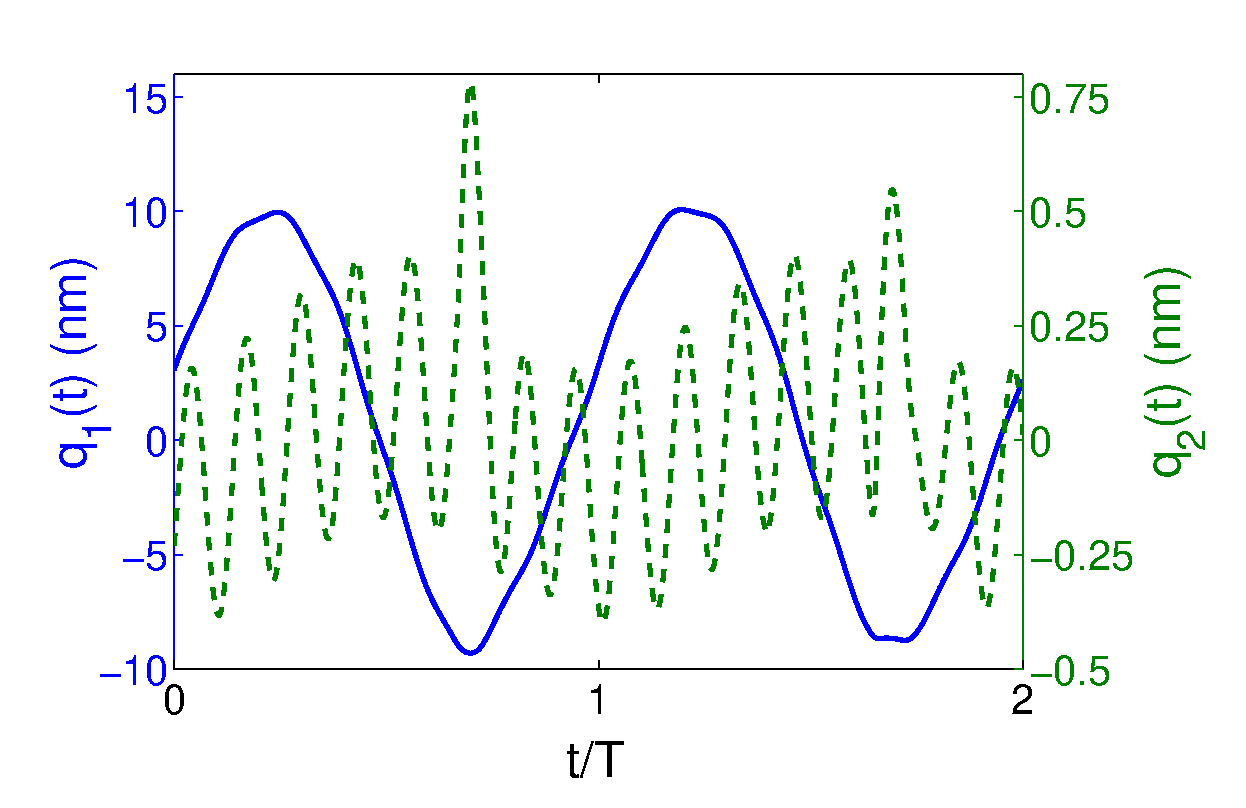
\includegraphics[width=3.5in]{ADACex2_Eig} \caption{Response of the first $q_{1}(t)$ and second $q_{2}(t)$ eigenmodes
of the cantilever at an amplitude ratio $A_{1}/A_{0}=0.9$. (\textbf{AMAC
Advanced} Example 2)}
\par\end{centering}
\centering{}\label{fig:ADACex2_Eig} 
\end{figure}



\subsubsection{\label{sec:Tools.DACAdvanced.Ex3}Example 3: Internal resonance of
a stiff cantilever in air}


In this example, we will simulate internal resonance of a stiff microcantilever
in air; this situation is commonly known as ``harmonic cantilevers''
in the AFM community. Internal resonance is a phenomenon that occurs
for special cantilevers in which a higher eigenmode, such as the second
flexural eigenmode or the first torsion mode, is very near an integer
multiple of the fundamental eigenmode \cite{Sahin_PRB_2004,Sahin_SA_2004,Sahin_RSI_2007,Sahin_NN_2007,Sahin_PRB_2008}.
This results in the higher eigenmode being excited by a harmonic of
the tip-sample interaction force. Refer to Table \ref{tab:ADACEx}
Example 3 for the correct input values for this example.

To begin this example, open the \textbf{AMAC Advanced} tool from the
\textbf{VEDA} tools selection. Wait for the user input window to open
(you should start in the \emph{Operating conditions and cantilever
properties} tab). Either select ``Example 3'' from the \emph{Example
Loader} dropdown box, or follow these instructions to set the parameters
manually: Change the \emph{excitation source} to \emph{Magnetic} and
set the \emph{Frequency scheme} to \emph{Single frequency (conventional)}.
Set the \emph{First frequency amplitude (nm)} to 20. Set the eigenmode
stiffness values (\emph{$k_{i}$ (N/m)}), and eigenmode quality factors
(\emph{Q}) to 30, 1200 and 400, 1200, respectively. Change the first
and second natural frequencies in (kHz) to 350, 2450, and change \emph{fd
(kHz)} to 350. Change the \emph{Z approach velocity (nm/s)} to 100.
Next, click on the \emph{Tip-sample interaction properties} tab. Under
this tab, change the \emph{Tip radius (nm)} to 10, and make sure the
\emph{Young's modulus of sample (GPa)} is set to 1 for the first simulation.
On the second run, the \emph{Young's modulus of sample (GPa)} will
be changed to 5. Set all non-conservative and forces to ``no'' or
``none''. Now, click on the \emph{Simulation parameters} tab. Set
the \emph{Number of points plotted} to 500. Check the \emph{Plot a
higher harmonic} box, and set the \emph{Number of higher harmonics}
to 1. Set the \emph{higher harmonic} to 7 only. Make sure the \emph{Include
sample of time histories} box is checked. Set the \emph{Number of
time histories to collect} to 1, and that the corresponding amplitude
ratio is 0.9 only. Set the \emph{Number of cycles included in sample}
to 2. Also, set the \emph{X-axis variable} to \emph{Amplitude ratio}
for this example.

Finally, click the \emph{Simulate} button in the lower right-hand
corner, and wait for the simulation to reach completion. Once the
simulation has completed, click the \emph{Input} button. Open the
\emph{Tip-sample interaction properties} tab, and change the \emph{Young's
modulus of sample (GPa)} to 5. Then, click the \emph{Simulate} button
again, and wait for the second simulation to reach completion. For
this example, each run generally takes about seven minutes to complete.
This gives a total running time of about 14 minutes.

Figure \ref{fig:ADACex3_DTS_E_s1} shows the key difference between
internal resonance in air for harmonic cantilevers, which is a steady
state resonant effect, and momentary excitation of higher eigenmode
for soft cantilevers in liquids shown in Figure \ref{fig:ADACex1_D_TS},
which is a transient ring-down effect that occurs because of low quality
factors inherent to soft cantilevers in liquids. For harmonic cantilevers
in air, which have high quality factors, the second eigenmode develops
a steady state {\em resonant} oscillation shown in Figure \ref{fig:ADACex3_DTS_E_s1}b.

The second eigenmode is excited by a harmonic of the tip-sample interaction
force and therefore contains information about tip-sample interaction
and thus the material properties of the sample. Unlike phase contrast
in air (See Figure \ref{fig:ADACex3_DTS_E_s2}), which tells only
about variations in dissipative (nonconservative) interactions, the
amplitude of the second eigenmode in an internal resonance scheme
contains information about conservative interactions. For the two
purely elastic samples (conservative tip-sample forces), there is
a clear contrast in the amplitude of the second 7th harmonic due to
the different elasticities.

\begin{figure}[htb]
\begin{centering}
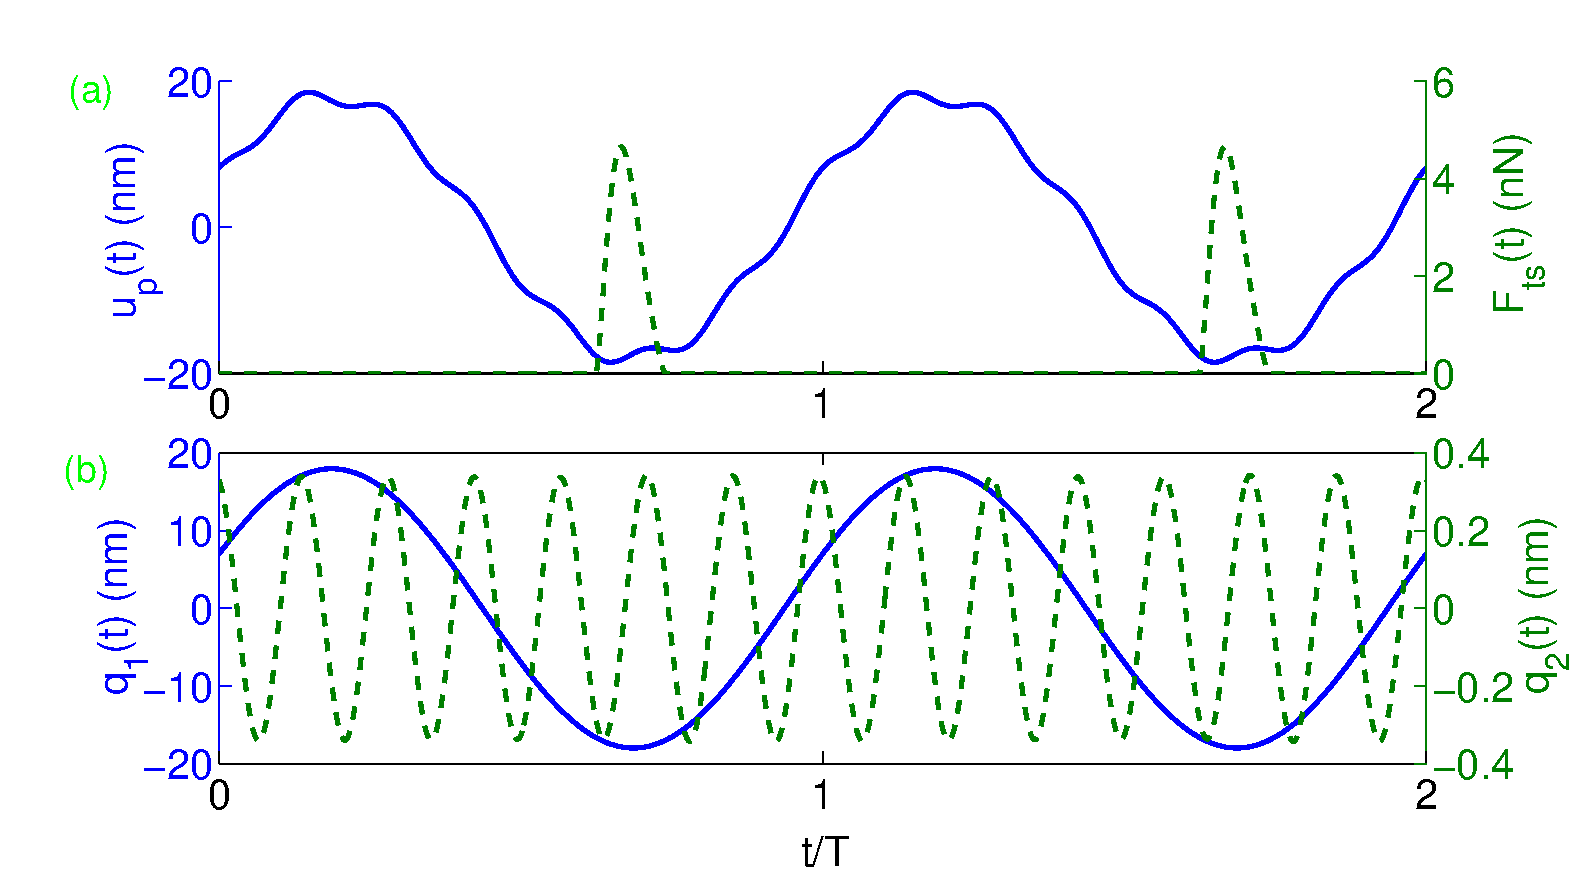
\includegraphics[width=3.5in]{ADACex3_DTS_E_s1} \caption{Internal resonance observed while tapping on a sample of $E=1$ GPa
at an amplitude ratio $A_{1}/A_{0}=0.9$. (a) Photodiode deflection
signal $u_{p}(t)$ and tip-sample interaction force $F_{ts}(t)$ vs.
time $t/T$ at $A_{1}/A_{0}=0.9$. (b) The first and second eigenmodes
at $A_{1}/A_{0}$=0.9. (\textbf{AMAC Advanced} Example 3)}
\par\end{centering}
\centering{}\label{fig:ADACex3_DTS_E_s1} 
\end{figure}

\begin{figure}[htb]
\begin{centering}
\includegraphics[width=3.5in]{ADACex3_DTS_E_s2} \caption{Internal resonance observed while tapping on a sample of $E=5$ GPa
at an amplitude ratio $A_{1}/A_{0}=0.9$. Photodiode deflection signal
$u_{p}(t)$ and tip-sample interaction force $F_{ts}(t)$ vs. time
$t/T$ at $A_{1}/A_{0}=0.9$. (b) The first and second eigenmodes
responses $A_{1}/A_{0}=0.9$. (\textbf{AMAC Advanced} Example 3)}
\par\end{centering}
\centering{}\label{fig:ADACex3_DTS_E_s2} 
\end{figure}

\begin{figure}[htb]
\begin{centering}
\includegraphics[width=4in]{ADACex3_A} \includegraphics[width=4in]{ADACex3_P}
\caption{(a) Amplitude $A_{1}$ (nm) or the primary harmonic of the excitation
frequency vs Z-distance for two different samples. (b) Phase of the
primary harmonic vs amplitude ratio $A_{1}/A_{0}$ where $A_{0}$
is the unconstrained amplitude. (c) Amplitude $A_{7}$ (nm) and (d)
phase (deg) of the $7^{th}$ harmonic vs amplitude ratio $A_{1}/A_{0}$
for two different samples. (\textbf{AMAC Advanced} Example 3)}
\par\end{centering}
\centering{}\label{fig:ADACex3_P} 
\end{figure}

\newpage{}



\subsubsection{\label{sec:Tools.DACAdvanced.Ex4}Example 4: Bimodal excitation in
air}


In this example, we will simulate a microcantilever excited in air
at its first two natural frequencies. To begin this example, open
the \textbf{AMAC Advanced} tool from the \textbf{VEDA} tools selection.
Wait for the user input window to open (you should start in the \emph{Operating
conditions and cantilever properties} tab). Either select ``Example
4'' from the \emph{Example Loader} dropdown box, or follow these
instructions to set the parameters manually: Change the \emph{excitation
source} to \emph{Magnetic} and set the \emph{Frequency scheme} to
\emph{two frequencies (bimodal)}. Set the unconstrained amplitude
\emph{$A_{0,1}$ (nm)} to 20 and set the \emph{Second frequency amplitude
(nm)} to 1.17. Then, set the equivalent stiffnesses of the eigenmodes
\emph{$k_{i}$ (N/m)}, and eigenmode quality factors \emph{$Q_{i}$}
to 30,1200 and 400,1200, respectively. Change the first and second
natural frequencies (kHz) and excitation frequencies (kHz) both to
$350,2250$, and change \emph{fd1 (kHz)} to 350. Set \emph{fd2 (kHz)}
to 2275. Change the \emph{Z approach velocity (nm/s)} to 100. Next,
click on the \emph{Tip-sample interaction properties} tab. Under this
tab, change the \emph{Tip radius (nm)} to 10, and make sure the \emph{Young's
modulus of sample (GPa)} is set to 1 for the first simulation. On
the second simulation, the \emph{Young's modulus of sample (GPa)}
will be changed to 5. Set the \emph{Sample viscosity ($Pa\cdot s$)}
to 0. Now, click on the \emph{Simulation parameters} tab. Set the
\emph{Number of points plotted} to 500. Uncheck the \emph{Plot a higher
harmonic} box. Make sure the \emph{Include sample of time histories}
box is checked. Set the \emph{Number of time histories to collect}
to 1, and that the corresponding amplitude ratio is 0.9 only. Set
the \emph{Number of cycles included in sample} to 4. Also, set the
\emph{X-axis variable} to \emph{Amplitude ratio} for this example.

Finally, click the \emph{Simulate} button in the lower right-hand
corner, and wait for the simulation to reach completion. Once the
simulation has completed, click the \emph{Input} button. Open the
\emph{Tip-sample interaction properties} tab, and change the \emph{Young's
modulus of sample (GPa)} to 5. Again, click the \emph{Simulate} button
and wait for the second simulation to complete. For this example,
each of the two simulations may take up to 6 minutes to complete for
a total running time of about 12 minutes.

Figure \ref{fig:ADACex4_DTS_E_s1} shows the waveform, tip-sample
interaction, and individual eigenmode responses for the first and
second eigenmode. Because of the high quality factors in air, the
momentary excitation of the second eigenmode is obviated and the waveform
is much less sporadic. However, the signal still does not evolve into
a periodic oscillation with respect to the drive frequency. Note the
slightly different tip-sample forces shown in Figure \ref{fig:ADACex4_DTS_E_s1}.

Unlike conventional single frequency tapping-mode, internal resonance,
and the first eigenmode of a bimodal scheme, we see that there is
phase contrast in the second eigenmode that occurs even for the purely
elastic samples (Figure \ref{fig:ADACex4_DTS_E_s2}). Additionally,
the amplitude contrast of the second eigenmode is inverted from internal
resonance (see Sec. \ref{sec:Tools.DACAdvanced.Ex3}, the stiffer
sample having a smaller amplitude.)

\begin{figure}[htb]
\begin{centering}
\includegraphics[width=4.5in]{ADACex4_DTS_E_s1} \caption{The cantilever response when approaching a sample of $E=1$ GPa. (a)
Photodiode deflection signal $u_{p}(t)$ and tip-sample interaction
force vs. Z-distance (nm) at $A_{1,1}/A_{0,1}$=0.9, where $A_{1,1}$
is the first harmonic or the primary excitation frequency and $A_{0,1}$
is the unconstrained amplitude at this frequency. (b) The response
of first and second eigenmodes at $A_{1,1}/A_{0,1}=0.9$. (\textbf{AMAC
Advanced} Example 4)}
\par\end{centering}
\centering{}\label{fig:ADACex4_DTS_E_s1} 
\end{figure}

\begin{figure}[htb]
\begin{centering}
\includegraphics[width=4.5in]{ADACex4_DTS_E_s2} \caption{The cantilever response when approaching a sample of $E=5$ GPa. (a)
Observed tip deflection and tip-sample interaction force vs. Z-distance
(nm) at $A_{1,1}/A_{0,1}=0.9$. (b) The first and second eigenmodes
at $A_{1}/A_{0}=0.9$. (\textbf{AMAC Advanced} Example 4)}
\par\end{centering}
\centering{}\label{fig:ADACex4_DTS_E_s2} 
\end{figure}

\begin{figure}[htb]
\begin{centering}
\includegraphics[clip,width=5in]{ADACex4_A} \includegraphics[clip,width=5in]{ADACex4_P}
\caption{(a) The amplitude $A_{1,1}$ (nm) of the first harmonic of the primary
excitation frequency vs Z distance for two different samples. (b)
Phase of the first harmonic of the primary excitation frequency vs.
amplitude ratio $A_{1,1}/A_{0,1}$ where $A_{0,1}$ is the unconstrained
amplitude of the primary frequency. The amplitude $A_{1,2}$ (nm)
(c) and phase (1,2) (d) of the primary harmonic of the \emph{second}
(bimodal) excitation frequency vs amplitude ratio $A_{1,1}/A_{1,0}$
for two different samples. (\textbf{AMAC Advanced} Example 4)}
\par\end{centering}
\centering{}\label{fig:ADACex4_P} 
\end{figure}



\subsubsection{\label{sec:Tools.DACAdvanced.Ex5}Example 5: Phase spectroscopy in
Bimodal AFM}

This example reproduces the results of \cite{lozano_prB_2009}. We
will attempt to show that bimodal AFM is sensitive to variations in
conservative attractive forces. Select example 5 from the dropdown
example loader and run the simulation. Then click back to tab 2 and
change the Hamaker constant from 4e-20 to 9e-20, and run the simulation.
Compare the two different results. In particular look at the 1st and
2nd frequency phase. Note that we are plotting these phases against
the 1st frequency amplitude ratio. Then, click back to tab 3, and
change the x-axis variable to \emph{2nd frequency amplitude ratio}.
Simulate both Hamaker constants. Examine the two phases now. Your
results should look like Figure \ref{fig:ADACex5}. You should find
contrast between the two materials when plotting the cross-mode representation.
That is, when you plot 2nd phase against 1st amplitude, or 1st phase
against 2nd amplitude, there is contrast between the two material.
But when you plot 1st phase versus 1st amplitude, or 2nd phase versus
2nd amplitude, the two materials look identical. Your simulation results
will likely show a little more noise than \cite{lozano_prB_2009}.
This is because we have picked a fast approach speed (100 nm/s) in
order to keep the simulation time short. Reducing the approach speed
will yield cleaner results.

\begin{figure}[htb]
\begin{centering}
\includegraphics[clip,width=5in]{ADAC_ex5_phase} \caption{Demonstration of bimodal sensitivity to conservative material properties.
The left column shows the parallel mode representation: 1st phase
vs 1st amp and 2nd phase vs 2nd amp. In this representation, both
materials have the same result (aside from a small amount of noise).
The right column shows the cross-mode representation, 1st phase vs
2nd amp and 2nd phase versus 1st amplitude. In this representation,
there is a very clear difference between the two materials. (\textbf{AMAC
Advanced} Example 5)}
\par\end{centering}
\centering{}\label{fig:ADACex5} 
\end{figure}



\subsection{\label{sec:AMS.adv}Amplitude Modulated Scanning (Advanced)}


The Advanced Amplitude Modulated Scanning builds upon the Basic Scanning
tool in the same way that the Advanced Amplitude Modulated Approach
Curves tool builds upon the Basic Amplitude Modulated Approach Curves.
Multiple eigenmodes, magnetic excitation, and other advanced features
are included. New users should first refer to the examples for the
Advanced Amplitude Modulated Approach curves tool and the Basic Amplitude
Modulated Scanning tool. All of the concepts in these tools are directly
transferable.



\subsubsection{\label{sec:AMS.adv.Ex1}Material Contrast in Bimodal AFM}


While imaging a two component-blend polymer sample with a tapping
mode cantilever in air, what types of material contrast can bimodal
AFM give between the two blends? Open the Amplitude Modulated Scanning
tool (advanced) and Load Example 1. This will set the parameters for
a small step feature on a substrate, initially the feature and the
substrate have the same material properties.

Before we run the bimodal case, let's run a plain tapping mode case.
Choose ``single frequency (conventional)'' from the dropdown box
``Choose frequency scheme'' on tab 1. Run this simulation and look
at the topography. By default, the feature has the same material properties
as the substrate. Now, click back and change the Feature Young's modulus
to 5 GPa on tab 4. Run this simulation. Examine the 1st harmonic phase.
Can you see any difference between the phase on the feature and on
the substrate?

You should notice two things. First, there is a topography error due
to the different stiffness of the feature. Second, there is no phase
contrast. Remember, phase in tapping mode depends on the RATIO of
dissipative to conservative forces. That ratio is zero for both cases
here because there is no dissipative component.

Now, change back to tab 1, and select Bimodal. You'll note that the
drive amplitudes and frequencies are already filled in for you. Run
this simulation. Examine second frequency amplitude and phase. You
should see a very clear contrast between the materials.

Experiment with different combinations of materials. What types of
contrasts can you see? \newpage{}



\subsection{\label{subsec:AM-SS}Amplitude Modulated Approach curves, steady
state solution}

\emph{THIS SECTION IS STILL UNDER CONSTRUCTION}

The basic idea of the tool is described in Ref \cite{rajabifar2018dynamic}.
This tool uses a completely different method than all of the other
tools. Instead of numerically solving the exact equations in time,
an single-harmonic steady state version is used. This is less accurate,
however in many situations can still provide a reasonable estimate
and is an order of magnitude faster than other tools. This was motivated
by the desire to simulate polymer surfaces using Attard's model (section
\ref{subsec:attard}). This model is computationally intractable for
the direct simulation used in the other tools, but runs in a reasonable
amount of time with this tool.

The basic options are similar to the other Amplitude Modulated Approach
Curves tools. Some exceptions are described below.

First, the excitation frequency is always assumed to be equal to the
natural frequency (i.e. on resonance operation). Second, for bimodal
operation, the tool needs to compute a number of cycles equal to the
lowest common multiple (aka as ``winding number'') of the two drive
periods. E.g. if the second frequency is 6.5 times the first, then
the winding number is 2 (i.e. the pattern repeats every 2 cycles of
the first frequency and every 13 cycles of the second frequency, because
13/2=6.5). If the ratio is 6.25 then the winding number is 4, and
if the ratio is 6.249, then the winding number is 1000 (6249/1000
= 6.249).

To avoid this number being excessive, the second drive frequency is
rounded. Two types of rounding are available. The first is ordinary
everyday rounding to either 1, 2 or 3 decimal places. For example
6.24 (156/25, winding number 25) could be rounded to 6.2 (31/5 winding
number 5). Although this is easy to understand, it may result in a
larger than necessary winding number (i.e. a slower simulation).

A more intelligent rounding is available. This looks for a pair integers
p, q such that p/q is approximately equal to the desired ratio and
q is no more than a specified limit. q is the winding number. E.g.
instead of rounding 6.24 down to 6.2 (winding number 5) with ordinary
rounding, we could round it up to 6.25, which has a winding number
of 4. This results in a simulation that is 20\% faster.

You can check the exact frequencies that were used by looking for
the ``Omega\_i (natural frequency)'' line in the ``Misc internal
values'' result.

The following examples are available
\begin{itemize}
\item Example 1: This is an identical set of parameters to Example 1 from
the Basic Amplitude Modulated Approach Curves tool, meant to illustrate
the differences between them. You should note that the steady state
tool runs an order of magnitude faster, and gets nearly the same result.
However, as the amplitude reduction must always be monotonic in this
tool, it misses a portion of the curve after the jump from attractive
to repulsive mode.
\item Example 2: This example illustrates using the tool on a conservative
sample, specifically capillary forces
\item Example 3: This example illustrates the use of Attard's model in tapping
mode, in repulsive regime. Examing the time history plots will show
the useful features of Attard's model.
\item Example 4: A second example of Attard's model, but this one is performed
in an attractive regime. Note in the time histories, the tip does
not indent the sample, rather you can see the sample rising up to
meet the tip.
\item Example 5: This example illustrates the use of bimodal on a conservative
sample (Hertz)
\item Example 6: This example illustrates the use of Attard's model in bimodal
\end{itemize}

\subsection{\label{sec:Tools.FrqSwp}Frequency Sweep}

In the process of imaging a sample, an AFM operator would typically
use a frequency sweep tuning curve to find a natural frequency (in
order to pick an operating frequency), and possibly to measure the
quality factor and/or stiffness of the given cantilever. In this case,
the frequency sweep performed far from the sample, and frequency response
is linear. To study nonlinear interactions with the sample, the cantilever
is brought closer to the sample so that the oscillating tip interacts
with the sample. The frequency sweep tool in VEDA is able to simulate
frequency sweeps while in interacting with the sample. This is useful
for gaining understanding of the underlying nonlinear dynamics of
AFM as well as understanding the operation of the instrument.

\subsubsection{\label{sec:Tools.FreqSweep.Ex1}Example 1: Examining the nonlinear
resonance response of a microcantilever near HOPG in air}

This example simulates the frequency response of an Olympus diving
board cantilever at various distances above HOPG in dry air. The parameters
for this simulation are taken from Lee, et al. \cite{Lee_PRB_2002}
and are given in Table \ref{tab:SweepEx}. In this example we will
investigate the nonlinear resonance response.

To begin this example, open the \textbf{Frequency Sweep} tool from
the \textbf{VEDA} tools selection. Start in the \emph{Operating conditions
and cantilever properties} tab. For \emph{excitation method} choose
\emph{Acoustic excitation}, for \emph{Excitation scheme}, choose \emph{Linear
ramp}, and uncheck the box \emph{Use setpoint}. Enter the values listed
in the table in the respective boxes. Then click the \emph{Tip-sample
interaction properties} tab. For \emph{Tip-sample interaction model}
select \emph{DMT contact}, and uncheck the box \emph{Auto Calculate
intermolecular distance}. Enter the values from the table in the respective
boxes. Then click simulate (the defaults in the \emph{Simulation parameters}
will be sufficient for this example.

The simulation should take approximately 20s. After the simulation
has run, click the input button in the lower left to go back to the
inputs. Select the \emph{Operating conditions and cantilever properties}
tab and increase the \emph{Unconstrained Amp @ Nat Freq (nm)} from
89.3 nm to 89.4 nm. Click the simulate tab. Repeat this process increasing
the unconstrained amplitude by 0.1 nm each time until a maximum of
90.2 nm (total 10 simulation runs).

Then, click the \emph{All} button to the right of the slider bar on
the graph window to plot all of the runs on top of each other. Then,
click and drag in the plot window to zoom in on the peak of the curves.
You should see a result like in Figure \ref{fig:SweepEx1_1}. This
figure is approximately the same as Fig 9 in Lee, et al., with three
exceptions. First, Lee, et al. plotted peak-peak amplitudes while
VEDA plots peak amplitudes, so the results are different by a factor
of two. Second, Lee, et al. did not use exactly 0.1 nm steps. Finally,
the paper was computed using AUTO97, which is able to find unstable
branches (the dashed lines in Figure 9 of Lee, et al. ). VEDA integrates
the differential equation numerically and so only the stable branches
can be plotted.

We note the following results about the plot. The lowest curve, representing
89.3 nm amplitude, is approximately the frequency response of a linear
single degree of freedom (DOF) oscillator. The separation 90 nm minus
the peak amplitude 89.3 nm yields a minimum tip-sample separation
of 0.7 nm during the oscillation. At this range the van der Waals
forces are almost zero, so there is little non-linear effect. With
each successive curve, the minimum tip-sample separation decreases,
so now van der Waals forces start to be significant. On each curve,
identify the point at which the maximum amplitude occurs. You will
notice that these points are decreasing in frequency as amplitude
increases. This is characteristic of a \emph{softening} non-linearity
(see, for example \cite{JordanSmith}). At 89.8 nm unconstrained amplitude,
the resonant peak will start to move up in frequency. This indicates
that the repulsive DMT forces are starting to have some effect. DMT
contact forces have a \emph{stiffening} effect. By 90.0 nm unconstrained
amplitude, the resonance peak has moved to the right of the original
resonant peak. If we draw a line connecting the resonance peaks for
each curve, we get the ``backbone'' curve, which is Figure 8 in
Lee, et al.

Let us use VEDA to examine some further features of this phenomena.
From the \emph{Result} drop down box, pick \emph{Mean Interaction
forces}. Drag \emph{Unconstrained Amp @ Nat Freq} slider bar from
left to right to highlight the curves one at a time. It should look
something like Figure \ref{fig:SweepEx1_2}. Notice that as the Unconstrained
amplitudes increase, the Mean forces become more and more negative
(attractive) until 89.8 nm. At 89.8 nm the mean force is still attractive
but it is has started to turn around and come back towards zero. At
90.0 you see that the mean force has become positive (repulsive) for
the first time. This is the transition between the so-called \textbf{attractive}
and \textbf{repulsive} imaging regimes.

Of course, in an real experiment we could not observe tip-sample interaction
force directly. But we can observe the phase of the response signal.
Choose \emph{First harmonic phase} from the drop down box, which will
look like Figure \ref{fig:SweepEx1_3}. For the curves in the attractive
regime, note that the phase angle increases (relative to the linear
case) as the frequency sweeps through resonance but for the curves
in the repulsive regime, the phase angle decreases.

\begin{table}[H]
\caption{\label{tab:SweepEx}Input parameters for Frequency sweep examples.}

\begin{ruledtabular} %
\begin{tabular}{lr}
~~~~\textbf{PARAMETER} & \textbf{EXAMPLE 1}\tabularnewline
\
~ & \tabularnewline
\textbf{Operating conditions, cantilever properties} & \tabularnewline
~~~~Choose excitation source & Acoustic\tabularnewline
~~~~Excitation scheme & Linear Ramp\tabularnewline
~~~~Number of eigenmodes & 1\tabularnewline
~~~~Unconstrained Amp. $@$ Nat. Freq.(nm) & 89.3\tabularnewline
~~~~Auto calculate $k_{i}~(i>1)$? & no\tabularnewline
~~~~$k_{i}$ (N/m) & 0.87\tabularnewline
~~~~$Q_{i}$ & 33.3\tabularnewline
~~~~Auto calculate Slope calibration? & yes\tabularnewline
~~~~$f_{1}$ (kHz) & 44\tabularnewline
~~~~$f_{dstart}$ (kHz) & 43.5\tabularnewline
~~~~$f_{dstop}$ (kHz) & 44.5\tabularnewline
~~~~Sweep time (s) & 0.1\tabularnewline
~~~~Tip mass, ($m_{tip}/m_{c}$) & 0\tabularnewline
~~~~Use setpoint & no\tabularnewline
~~~~Z distance (nm) & 90\tabularnewline
~ & \tabularnewline
\textbf{Tip-sample interaction properties} & \tabularnewline
~~~~Tip-sample interaction model & DMT contact\tabularnewline
~~~~Tip radius (nm) & 10\tabularnewline
~~~~Young's modulus of tip (GPa) & 130\tabularnewline
~~~~Poisson's ratio of the tip & 0.3\tabularnewline
~~~~Auto Calculate intermolecular distance? & no\tabularnewline
~~~~Intermolecular distance (nm) & 0.38\tabularnewline
~~~~Hamaker constant (J) & 2.96e-19\tabularnewline
~~~~Young's modulus of sample (GPa) & 10\tabularnewline
~~~~Poisson's ratio of the sample & 0.3\tabularnewline
~ & \tabularnewline
\textbf{Simulation parameters} & \tabularnewline
~~~~Number of points plotted & 1000\tabularnewline
~~~~Deflection points per cycle & 1000\tabularnewline
\end{tabular}\end{ruledtabular} 
\end{table}

\begin{figure}[htb]
\begin{centering}
\includegraphics[width=5in]{SweepEx1_1} \caption{First harmonic amplitude versus frequency for 10 different unconstrained
amplitudes. The series of curves illustrates the softening (due to
van der Waals) and then hardening (due to DMT contact) backbone curve
(\textbf{Frequency Sweep} Example 1)}
\par\end{centering}
\centering{}\label{fig:SweepEx1_1} 
\end{figure}

\begin{figure}[htb]
\begin{centering}
\includegraphics[width=5in]{SweepEx1_2} \caption{Mean interaction force versus frequency for 10 different unconstrained
amplitudes. The series of curves illustrates the transition from the
attractive regime to the repulsive regime (\textbf{Frequency Sweep}
Example 1)}
\par\end{centering}
\centering{}\label{fig:SweepEx1_2} 
\end{figure}

\begin{figure}[htb]
\begin{centering}
\includegraphics[width=5in]{SweepEx1_3} \caption{First harmonic phase versus frequency for 10 different unconstrained
amplitudes. The series of curves illustrates the transition from the
attractive regime to the repulsive regime (\textbf{Frequency Sweep}
Example 1)}
\par\end{centering}
\centering{}\label{fig:SweepEx1_3} 
\end{figure}



\subsubsection{\label{sec:Tools.FreqSweep.Ex1}Example 2: Effect of sample Stiffness
on non-linear response}


In this example, we will determine the effect of sample stiffness
on the non-linear frequency response that we found in the previous
example. This example will use the same basic parameter set as Example
1. If you have just run example 1, then hit the ``Clear'' button
in the outputs window to delete the old results and then go back to
the Simulation. If you are starting this example fresh, follow the
instructions to in Example 1 to input the first set of parameters,
or use the Example Loader to get the first set of parameters. Make
sure the Unconstrained Amplitude is 90.2 nm. Then in the simulation
tab, change the Young's modulus to 5 GPa and hit the ``simulate''
button. Once the simulation has run, return the to inputs window and
change Young's modulus to 10 GPa. Repeat for 15, 20, and 25 GPa.

Hit the ``All'' button to overlay the results. If you zoom in a
little bit, the output window should look like Figure \ref{fig:SweepEx2_1}.
You will notice that the jump-down happens farther to the right for
stiffer samples. That is, there is a larger range of frequencies where
non-linear effects are important. This is a general trend in AFM:
Tip-sample non-linearities are more pronounced for stiffer samples.

\begin{figure}[htb]
\begin{centering}
\includegraphics[width=5in]{SweepEx2_1} \caption{First harmonic amplitude versus frequency for 5 different sample Young's
moduli (\textbf{Frequency Sweep} Example 2)}
\par\end{centering}
\centering{}\label{fig:SweepEx2_1} 
\end{figure}



\subsubsection{\label{sec:Tools.FreqSweep.Ex1}Example 3: Sweep up versus sweep
down}


In this example, we will examine the difference between sweep up (starting
at a low frequency and gradually increasing the frequency) and sweep
down (starting at a high frequency and gradually decreasing the frequency).
For a linear system, these two are always identical, but for a non-linear
system they may be quite different. This example will use the same
basic parameter set as Examples 1 and 2. If you have just run example
1 or 2, then hit the ``Clear'' button in the outputs window to delete
the old results and then go back to the Simulation. If you are starting
this example fresh, follow the instructions to in Example 1 to input
the first set of parameters, or use the Example Loader to get the
first set of parameters. Make sure the Unconstrained Amplitude is
90.2 nm, and set the sample Young's modulus to 15 GPa and hit the
``simulate'' button. Once the simulation has run, return the to
inputs window and reverse fd start and fd stop (i.e. set fd start
= 44.5 and set fd stop = 43.5 kHz). Then hit simulate again. Hit the
``All'' button to overlay the two results.

You will notice that the sweep up and sweep down are close to each
other, except for a small region in the middle. If you zoom in on
this region, the output window should look like Figure \ref{fig:SweepEx3_1}.
First, examine the responses at 44.2 kHz. At this frequency, the sweep
up and sweep down simulations have very different amplitudes. This
mean that at this particular combination of Z, unconstrained amplitude,
and drive frequency, there are two different possible solutions. Which
solution you get depends on the initial conditions (i.e. where you
are coming from). Note that this condition, refered to as bi-stability,
can be undesirable for imaging. Bi-stabilities are explored more in
the Amplitude Modulated Approach Curves examples.

Now, examine the response at 44.3 kHz. There is also a small difference
between sweep up and sweep down here. Is this also due to a non-linear
effect? No. This is a linear effect due to the fact that we are changing
frequency at a fairly rapid rate (change of 1 kHz in 0.1s) so that
the system is not quite at steady state. If you were to repeat this
simulation but with a sweep time of 0.5s instead, there should be
much better agreement at 44.3 kHz, but of course that simulation will
take five times longer to run. You might also notice that the jump-downs
will be sharper (higher slope) at the slow sweep rate, and might happen
at slightly different frequencies.

\begin{figure}[htb]
\begin{centering}
\includegraphics[width=5in]{SweepEx3_1} \caption{First harmonic amplitude versus frequency for sweep up versus sweep
down (\textbf{Frequency Sweep} Example 3)}
\par\end{centering}
\centering{}\label{fig:SweepEx3_1} 
\end{figure}

\newpage{}



\subsection{\label{sec:Tools.FZcurves}Force Distance Curves}

This tool simulates approach and retraction curves between the tip
of an unexcited cantilever and a sample.

The following assumptions are unique to the F-Z Curves tool: 
\begin{enumerate}
\item The cantilever is unexcited (forcing function applied to the cantilever).
Any tip deflections would be caused by interactions between the tip
and sample only. 
\item Interactions between the tip and the sample are modeled by any one
of the models described in Section \ref{sec:fts}. 
\item The $Z$ separation between the sample can be reduced or increased,
but the cantilever does not move laterally.
\item Inertial forces caused by the $Z$ motion are negligible (but viscous
forces are included)
\end{enumerate}
The curves may be triggered (approach to a specific deflection and
then reverse) or untriggered (approach to a specific Z distance and
then reverse).

This section provides an overview of the outputs of the F-Z Curves
(FZC) tool in the form of several example simulations. 
\begin{table}[H]
\caption{\label{tab:FZcurvesEx}Input parameters for F-Z Curves examples.}

\begin{ruledtabular} %
\begin{tabular}{lrr}
~~~~\textbf{PARAMETER} & \textbf{EXAMPLE 1} & \textbf{EXAMPLE 2}\tabularnewline
~ &  & \tabularnewline
\textbf{Operating conditions and cantilever properties} &  & \tabularnewline
Operating mode & \multicolumn{2}{r}{Untriggered, Approach \& Retract}\tabularnewline
~~~~Number of eigenmodes & 1 & 1\tabularnewline
~~~~Auto calculate $k_{i}~(i>1)$? & no & no\tabularnewline
~~~~$k_{i}$ (N/m) & 0.87 & 0.87\tabularnewline
~~~~$Q_{i}$ & 33 & 33\tabularnewline
~~~~$f_{i}$ (kHz) & 44 & 44\tabularnewline
~~~~Tip mass & 0 & 0\tabularnewline
~~~~Z approach velocity (nm/s) & 200 & 200\tabularnewline
~~~~Gamma (Z drag) & 0 & 0\tabularnewline
~~~~Initial Z separation (nm) & 10 & -5\tabularnewline
~~~~Final Z separation (nm) & -5 & 10\tabularnewline
~ &  & \tabularnewline
\textbf{Tip-sample interaction properties} &  & \tabularnewline
~~~~Tip-sample interaction model & DMT contact & JKR\tabularnewline
~~~~Tip radius (nm) & 10 & 10\tabularnewline
~~~~Young's modulus of tip (GPa) & 130 & 130\tabularnewline
~~~~Poisson's ratio of the tip & 0.3 & 0.3\tabularnewline
~~~~Auto calculate intermolecular distance? & yes & NA\tabularnewline
~~~~van der Waals adhesion force (nN) & 1.4167 & 1.4167\tabularnewline
~~~~Hamaker constant (J) & $3.4\cdot10^{-20}$ & NA\tabularnewline
~~~~Young's modulus of sample (GPa) & 1 & 1\tabularnewline
~~~~Poisson's ratio of the sample & 0.3 & 0.3\tabularnewline
~ &  & \tabularnewline
\textbf{Simulation parameters} &  & \tabularnewline
~~~~Number of points plotted & 1000 & 1000\tabularnewline
~~~~Deflection points per cycle & 1000 & 1000\tabularnewline
\end{tabular}\end{ruledtabular} 
\end{table}

\newpage{}

\subsubsection{\label{sec:Tools.FZcurves.Ex1}Example 1: Approaching and retracting
from a sample modeled using DMT contact}

The primary experimental observable in this type of experiment is
tip deflection versus Z displacement, and this is shown in Figure
\ref{fig:FZex1_deflZ}. Typically this deflection is then multiplied
by the cantilever static bending stiffness to arrive at tip-sample
interaction force versus Z displacement. Since this is a simulation,
we have the tip-sample force available to us directly, see figure
\ref{fig:FZex1_FtsZ}. Note that there appears to be some ringing
of the cantilever on snap-in. This is because VEDA is simulating the
entire cantilever dynamics in the time-domain, it is not a static
solution. Two quantities that are often of interest in force spectroscopy
are tip-sample interaction force versus gap and indentation versus
Z displacement. In an experiment these would have to be reconstructed
from the observed deflection, but since this is a simulation, we have
them directly in Figures \ref{fig:FZex1_FtsD} and \ref{fig:FZex1_IZ}.

\begin{figure}[htb]
\begin{centering}
\includegraphics[clip,width=5in]{FZex1_deflZ} \caption{Observed cantilever tip deflection versus Z-distance for the unexcited
cantilever (modeled using DMT contact). (FZ Curves Ex. 1)}
\par\end{centering}
\centering{}\label{fig:FZex1_deflZ} 
\end{figure}

\begin{figure}[htb]
\begin{centering}
\includegraphics[width=3.5in]{FZex1_FtsZ} \caption{Tip-sample interaction force versus Z-distance for the unexcited cantilever
(modeled using DMT contact). (FZ Curves Ex. 1)}
\par\end{centering}
\centering{}\label{fig:FZex1_FtsZ} 
\end{figure}

\begin{figure}[htb]
\begin{centering}
\includegraphics[clip,width=5in]{FZex1_FtsD} \caption{Tip-sample interaction force versus gap for the unexcited cantilever
(modeled using DMT contact). (FZ Curves Ex. 1)}
\par\end{centering}
\centering{}\label{fig:FZex1_FtsD} 
\end{figure}

\begin{figure}[htb]
\begin{centering}
\includegraphics[width=3.5in]{FZex1_IZ} \caption{Tip indentation into sample versus Z-distance for the unexcited cantilever
(modeled using DMT contact).(FZ Curves Ex. 1)}
\par\end{centering}
\centering{}\label{fig:FZex1_IZ} 
\end{figure}

\newpage{}

\subsubsection{\label{sec:Tools.FZcurves.Ex2}Example 2: Approaching and retracting
from a sample modeled using JKR}

This example uses the exact same parameters as Example 1, except the
sample is modeled using JKR contact instead of DMT. Assuming you have
already run example 1, go back to tab 2, change the interaction model
to JKR and then simulate again. Compare the results for the two different
interaction models. When you examine the cantilever deflection versus
Z (Figure \ref{fig:JKRex2_FtsZ}) you will note that during the approach,
the cantilever tip snaps onto the sample later using the JKR model
than with the DMT contact model. The reason for this is the discontinuous
jump in the force seen in JKR, whereas the DMT contact model utilized
an attractive van der Waals force even before the cantilever tip contacts
the sample.

\begin{figure}[htb]
\begin{centering}
\includegraphics[width=3.5in]{JKRex2_FtsZ} \caption{Tip-sample interaction force versus Z-distance for the unexcited cantilever
(modeled using JKR). (FZ Curves Ex. 2)}
\par\end{centering}
\centering{}\label{fig:JKRex2_FtsZ} 
\end{figure}

\begin{figure}[htb]
\begin{centering}
\includegraphics[width=3.5in]{JKRex2_deflZ} \caption{Observed cantilever tip deflection versus Z-distance for the unexcited
cantilever (modeled using JKR).(FZ Curves Ex. 2)}
\par\end{centering}
\centering{}\label{fig:JKRex2_deflZ} 
\end{figure}

\begin{figure}[htb]
\begin{centering}
\includegraphics[width=3.5in]{JKRex2_IZ} \caption{Tip indentation into sample versus Z-distance for the unexcited cantilever
(modeled using JKR).(FZ Curves Ex. 2)}
\par\end{centering}
\centering{}\label{fig:JKRex2_IZ} 
\end{figure}


\subsubsection{Example 3: Approaching and retracting from a sample using Attard's
model}

This example demonstrates the use of Attard's model for viscoelasticity
(Section \ref{subsec:attard}). As this model is more complex than
other models, an additional visualization has been included: a movie
showing the interaction of the tip with the sample surface. This is
located under ``Surface Deformation Movie''

\begin{figure}
\includegraphics{Fz_ex3_DvZ}

\caption{Observed cantilever deflection vs Z distance for a soft sample modeled
using Attard's model (Fz curves Ex 3)}

\end{figure}

\begin{figure}
\includegraphics{AttardMovie}

\caption{Surface deformation movie. The top line is the tip and the bottom
line is the sample. (Fz curves Ex 3)}

\end{figure}

\newpage{}

\subsection{\label{sec:Tools.ForceViewer}Force Viewer}

In order to run a simulation, it is necessary to specify a tip-sample
interaction model. Cartoons of representative tip-sample interaction
models are given in section \ref{sec:fts}. It is often useful, however,
to see the exact tip-sample force vs. gap curve for a specific set
of parameters. The F-Z curves tool can be used for this (e.g. Figure
\ref{fig:FZex1_FtsD}), however the problem with that tool is that
since it simulates the cantilever dynamics, some regions of the F-d
curve are not visible. That is, when the cantilever snaps-in or pulls-off,
it skips over a region in the F-d curve. The force-viewer tool is
utility that does not have this deficiency. It plots the entire F-d
curve independent of any cantilever dynamics.

\subsubsection{Example 1: DMT Model}

As an example, we shall plot the tip-sample interaction force for
the parameter of F-Z curves Example 1. Open the Force Viewer tool
from the VEDA tools menu. Enter 5 nm for the starting gap, -0.9 for
the final gap. On the Tip-sample interaction tab, enter the parameters
from Table \ref{tab:FZcurvesEx} Example 1. Press simulate. You should
get an output like Figure \ref{fig:FViewEx1_FtsD}. Compare this with
Figure \ref{fig:FZex1_FtsD}. The two figures should be identical,
except Figure \ref{fig:FViewEx1_FtsD} contains the entire curve in
the area where Figure \ref{fig:FZex1_FtsD} had a blank spot.

The force viewer also plots the interaction stiffness, which is the
first derivative of the interaction force. This is useful for comparision
to many small-amplitude spectroscopy theories which calculate interaction
stiffness (e.g. \cite{debeer2010dissipation}). Note that the sign
convention on interaction stiffness is typically taken such that a
positive interaction stiffness causes a positive shift in resonance
frequency. In other words, $k_{int}=-\frac{\partial}{\partial d}F_{ts}(d)$.
Versions of VEDA prior to 2.0.19 (Feb 2011) used the opposite sign
convention (positive gradient causes negative frequency shift, which
is not as commonly used in the literature).

\begin{figure}[htb]
\begin{centering}
\includegraphics[clip,width=5in]{FViewEx1_FtsD} \caption{Tip-sample force versus gap (modeled using DMT). Force Viewer Ex.
1}
\par\end{centering}
\centering{}\label{fig:FViewEx1_FtsD} 
\end{figure}


\subsubsection{Example 2: Viscoelastic Material Models}

The force viewer tool can also be used to explore non-conservative
forces. In this case, the forces when approaching the sample are different
than the forces retracting from the sample. In this example, we demonstrate
using the tip-sample force viewer to see the forces when a Prony series
model is used.

We start with the DMA (Dynamic Mechanical Analysis) data of Read \cite{Read1989}
for polypropylene. The raw data is reproduced in Figure \ref{fig:Read_polymer}.
This data is specified as $E_{loss}$ and $E_{storage}$ versus frequency,
which is typical for DMA data. VEDA cannot directly utilize this type
of data. Instead, we must fit the data to one of the constitutive
models in section \ref{sec:fts}. In this case we use a Prony series
(Generalized Maxwell) section \ref{subsec:Prony}. The Prony series
consists of a set of pairs of modulii $G_{j}$ and relaxation times
$\tau_{j}$. To do the fit, we specify the $\tau_{j}$ a priori, and
then use a least squares fit to calculate the modulii $G_{j}$ that
best fit the data.

In this case we choose to use a seven term series (more terms will
fit the data better, but obviously will take longer to simulate).
We anticipate running a simulation with a 100 kHz cantilever which
will have a contact time of a few microseconds, so we choose the relaxation
times equally spaced (on a logarhythmic scale) between 2 ms and 0.1
us, which gives relaxation time spaced above and below the expected
contact time. The fit is conducted using lsqcurvefit() command in
Matlab. You can use the ``Fit Viscoelastic DMA data to Prony Series''
tool to do these fits on your own data.

The results are shown in figure \ref{fig:Read_polymer_fit}. As you
can tell, the Prony series fits the data reasonable well between 100
Hz and 1 MHz. A better fit could have been obtained with more terms,
but this is not bad for an example.

Now we will see the forces that result from indenting this sample.
Open the force viewer tool and select Example 2 from the drop down
box. You'll note that the Non-conservative velocity option has been
set to a sine wave with duration 10 microseconds, and that the initial
gap is set just above zero. This approximately simulates a contact
time of 10 us. On the tip-sample interaction tab, you'll note that
the Prony series coefficients have been filled in at the bottom under
Non-conservative forces. Click to simulate a single tap with these
parameters. Then, go back to tab 1 and decrease the time from 10 microseconds
to 0.1 microsecond and re-run.

The results are shown in Figure \ref{fig:Forceviewer_prony}

\begin{figure}
\centering{}\includegraphics[clip]{Read_polymer} \caption{\label{fig:Read_polymer}DMA data from \cite{Read1989} for polypropylene.
Force Viewer Ex. 2}
\end{figure}

\begin{figure}
\centering{}\includegraphics[clip]{read_estorage_fit} \includegraphics[clip]{read_eloss_fit}
\caption{\label{fig:Read_polymer_fit}Prony series fit to dma data. Force Viewer
Ex. 2}
\end{figure}

\begin{figure}
\centering{}\includegraphics[clip]{forceviewer_prony} \caption{S\label{fig:Forceviewer_prony}imulation of a single tap on a polymer
at two different rates. Force Viewer Ex. 2}
\end{figure}


\subsection{\label{sec:Tools.FMAC}FM Approach Curves}

\subsubsection{\label{sec:Tools.FMAC_Ex1}Approach to a Si facet in UHV}

In this example we simulate the approach of a silicon tip onto a (111)
silicon facet. The majority of the parameters are taken from \cite{Nony_PRB_2006}.
The only difference is that Nony's controller scheme is slightly different,
so we have used controller gains appropriate to VEDA's controller.

Launch the Frequency Modulated Approach Curves tool and enter the
parameters shown in Table \ref{tab:FMACEx}. The majority of the parameters
are similar to those in the Amplitude Modulated Approach Curves tool
so we will only walk through a few of the parameters.

The Frequency Modulation tab is unique to the FM tools. On it you
will find the controller gains for the frequency modulation controllers.
Chose Direct Amp/Freq Control yes (see section \ref{sec:theory.FM-CTRLdyn}
). We have implemented the method of \cite{Kilpatrick2009} to automatically
calculate gains for the PLL and amplitude controller. Leave this box
checked to get a good starting guess for the gains. After the simulation
has run, you can see the gains that were calculated in the \emph{Misc.
Internal Values} result, and use them as starting values if you want
to tweak the controller performance.

The simulation parameters tab contains one difference from the AM
tools. For the AM tools, it was possible to plot most variables against
either Z displacement or setpoint ratio. For FM, setpoint ratio does
not exist because amplitude is constant. Therefore, the options are
Z displacement and min gap (also known as the ``distance of minimum
approach'' in the literature). Choose min gap for this simulation
to compare with Nony's results.

Hit the simulate button and wait for the simulation to run. Note that
this simulation does take several minutes to run. If you are short
on time, you can increase the approach speed to 20 nm/s. The results
will be slightly off, but the general picture will be okay.

The first thing you should check in any frequency modulation approach
curve is the the controller performance. Examine the first harmonic
amplitude and first harmonic phase. You will want to verify that the
these two parameters stay relatively constant during the approach.
The phase is shown in Figure \ref{fig:FMAC_Ex1_Phase}. In this case
phase is constant to within about 0.1 degree during the majority of
the approach and starts to deviate at the very end (where the Morse
potential starts changing very rapidly). The amplitude controller
also performs well, about 0.1 percent deviation over the entire range.
This controller performance should be acceptable. When you start to
run your own simulations, always check these two parameters. If the
first harmonic amplitude or phase starts to deviate from a straight
line, you'll need to tune the controller parameters. If these drop
significantly, you may need to increase the gains. If they start a
growing oscillation, you may need to decrease the gains. You will
need to reconsider the gains any time you change a parameter, but
especially approach speed, quality factor, lock-in parameters, sampling
rate, and natural frequencies

Now, examine the FM Feedback results. This contains the two main FM
observables. The frequency shift is of most interest. The shape of
the frequency shift follows the tip-sample interaction force. In fact,
the exact tip-sample interaction force should be recoverable from
the frequency shift (see \cite{Sader_APL_2004}). The other channel
is the drive amplitude, which is sometimes called the ``apparent
dissipation'' or sometimes just ``dissipation.'' In this case,
the Morse potential is a purely conservative interaction, so there
is no actual dissipation there. However, the driving frequency is
changing, and the energy dissipation of a simple harmonic oscillator
changes with the drive frequency. This is one contribution to the
apprent dissipation. A second component is the small phase error we
noted before. A phase error indicates that the PLL is not exactly
tracking the natural frequency, and when driving off resonance more
energy is required. To reduce this error, we could decrease the approach
speed to give the PLL more time to react.

\begin{figure}[htb]
\begin{centering}
\includegraphics[clip,width=5in]{FMAC_Ex1_phase} \caption{First harmonic phase versus min gap during the approach curve. The
phase stays relatively constant during most of the approach, indicating
a good controller. Near the left side of the figure, the change in
phase indicates that the controller cannot keep up as well in this
region. FMAC Ex. 1}
\par\end{centering}
\centering{}\label{fig:FMAC_Ex1_Phase} 
\end{figure}

\begin{figure}[htb]
\begin{centering}
\includegraphics[clip,width=5in]{FMAC_Ex1_FMFeedback} \caption{Frequency shift (blue) and Drive Amplitude (red) (aka apparent dissipation)
during the approach curve. FMAC Ex. 1}
\par\end{centering}
\centering{}\label{fig:FMAC_Ex1_FMFeedback} 
\end{figure}

\begin{table}[H]
\caption{\label{tab:FMACEx}Input parameters for Frequency Modulated approach
curve examples.}

\begin{ruledtabular} %
\begin{tabular}{lrr}
~~~~\textbf{PARAMETER} & \textbf{EXAMPLE 1} & \textbf{EXAMPLE 2}\tabularnewline
\
~ &  & \tabularnewline
\textbf{Operating conditions, cantilever properties} &  & \tabularnewline
~~~~Choose excitation source & Acoustic & magnetic\tabularnewline
~~~~Choose frequency scheme & Single Frequency & Single Frequency\tabularnewline
~~~~Number of eigenmodes & 1 & 2\tabularnewline
~~~~Unconstrained Amp. $@$ Nat. Freq.(nm) & 7.0 & 1\tabularnewline
~~~~Auto calculate $k_{i}~(i>1)$? & no & yes\tabularnewline
~~~~$k_{i}$ (N/m) & 30 & 0.6\tabularnewline
~~~~$Q_{i}$ & 100 & 3,4\tabularnewline
~~~~$f_{1}$ (kHz) & 150 & 10,70\tabularnewline
~~~~$f_{d}$ (kHz) & 150 & 10\tabularnewline
~~~~Tip mass, ($m_{tip}/m_{c}$) & 0 & 0\tabularnewline
~~~~Approach velocity (nm/s) & 2 & 5\tabularnewline
~~~~Initial Z separation (nm) & 9.5 & 3\tabularnewline
~~~~Final Z separation (nm) & 7.1 & 0.5\tabularnewline
~~~~Choose Lock-in filter order & 4th order & 2nd order\tabularnewline
~~~~Lock-in time constant & 50 us & 1 ms\tabularnewline
~~~~Sampling frequency (MHz) & 0.5 & 1\tabularnewline
~ &  & \tabularnewline
\textbf{Frequency Modulation} &  & \tabularnewline
~~~~Direct Amp/Phase Control & yes & yes\tabularnewline
~~~~Autocalculate Controller gains & yes & yes\tabularnewline
\textbf{Tip-sample interaction properties} &  & \tabularnewline
~~~~Tip-sample interaction model & Morse Potential + van der Waals & Hertz\tabularnewline
~~~~Tip radius (nm) & 5 & 5\tabularnewline
~~~~Hamaker constant(J) & 1.865e-19 & NA\tabularnewline
~~~~Morse equilibrium position(nm) & 0.2357 & NA\tabularnewline
~~~~Morse range(nm) & 0.12 & NA\tabularnewline
~~~~Morse depth(J) & 3.641e-19 & NA\tabularnewline
~~~~Young's modulus of sample & 60 & \tabularnewline
~~~~Poisson's ratio of the sample & 0.3 & \tabularnewline
~~~~Include hydration forces & no & yes\tabularnewline
~~~~Lambda & NA & 0.245\tabularnewline
~~~~Hydration scaling & NA & 1.2e7\tabularnewline
~~~~Non-conservative solvation forces & no & yes\tabularnewline
~~~~Scaling & NA & 1e-5\tabularnewline
~~~~Decay & NA & 0.25\tabularnewline
~ &  & \tabularnewline
\textbf{Simulation parameters} &  & \tabularnewline
~~~~Number of points plotted & 1000 & \tabularnewline
~~~~Deflection points per cycle & 1000 & \tabularnewline
~~~~Choose x-axis variable & Min gap & \tabularnewline
~~~~use defaults for all other parameters on this tab &  & \tabularnewline
\end{tabular}\end{ruledtabular} 
\end{table}



\subsubsection{\label{sec:Tools.FMAC_Ex2}Approach to mica in liquid}

This example is under construction

\subsection{\label{sec:Tools.FMScan}FM Scanning}

The FM scanning tool combines the functionality of the other scanning
tools with the frequency modulation discussed under FM Approach Curves.
The only additions are that there is now a frequency shift setpoint
on tab 2 (you can specify if this should be an attractive or repulsive
shift).

It is recommended to use autocalculation of the Amplitude and PLL
gains when using this tool. If you wish to use non-default gains,
it is suggested that you use the FM Approach curves tool to find stable
gains first, then move on to this tool. Otherwise if you have stability
problems, it will be difficult to determine if the problem is with
your Z (topography) gains or with the FM gains.

There are currently no examples for the FM Scanning tool.

\subsection{\label{sec:Tools.ContactScan}Contact Mode Scanning}

The contact mode scanning tool simulates one of the earliest and simplest
AFM imaging modes. The utility of this tool is that allows understanding
the operation of the controller without having to deal with the complexities
of dynamic AFM.

\subsubsection{Example 1: Tip-sample geometry convolution}

This example illustrates the tip-sample geometry convolution described
in section \ref{sec:theory.TSgeom_conv}. Select example 1 from the
drop down menu. On the tip-sample interaction properties tab, note
that we have picked a 5 nm tip radius. The end of the tip is assumed
to be spherical. Also, on the feature properties tab, we've picked
a sinusoidal feature with height 30 nm and width 35 nm and checked
the box for tip-sample convolution.

Click simulate to begin the simulations. When it's done, the result
should look like \ref{fig:scancontact_Ex1_1}. The measured topography
(blue) resembles the actual sample geometry (red), but it is just
slightly wider. This is a common problem with measuring widths of
small features.

Go back to the feature properties tab and reduce the feature width
to 25 nm. Repeat the simulation for feature widths of 15, 5, and 1
nm. When you're finished the result should look some like Figure \ref{fig:scancontact_Ex1_2}.
Note that we've turned off the ``sample height'' plots to improve
clarity (click on the triangle to reveal the legend, and uncheck all
the red lines). Note that as the feature width decreases, the measured
geometry looks less and less like a sinusoid, and more like a rectangle
a circle of radius 5 nm on top (draw in dashed line for illustration).
In this case, the sample is showing us an image of the tip, instead
of the tip showing us an image of the sample!

\begin{figure}[htb]
\begin{centering}
\includegraphics[clip,width=0.9\textwidth]{scancontact_ex1_1} \caption{Measured topography for a 5 nm tip radius compared with the actual
sinusoidal feature of width 35 nm. The measured topography resembles
the feature, but is just slightly wider.}
\par\end{centering}
\centering{}\label{fig:scancontact_Ex1_1} 
\end{figure}

\begin{figure}[htb]
\begin{centering}
\includegraphics[clip]{scancontact_ex1_2} \caption{Measured geometry for a 5 nm tip radius and a sinusoidal feature of
successively decreasing widths. For very small features, the measured
geometry begins to resemble a circle with a radius of 5 nm - the feature
is imaging the tip instead of the tip imaging the feature}
\par\end{centering}
\centering{}\label{fig:scancontact_Ex1_2} 
\end{figure}


\subsection{Peak force tapping tool}

\emph{THIS SECTION IS STILL UNDER CONSTRUCTION}

The peak force tapping tool simulates the scanning mode of the same
name (https://www.bruker.com/content/bruker/int/en/products-and-solutions/microscopes/materials-afm/afm-modes/peakforce-tapping.html).
In this mode, the Z piezo is oscillated at a frequency considerably
lower than the cantilever resonance, e.g. 2 kHz for a 100 kHz cantilever.
Effectively this collects a series of force-distance curves. For each
curve, the deflection is processed to extract the peak force, and
then a feedback control is used to adjust the mean Z position such
that the peak force is constant over the scan.

Major assumptions of this tool:
\begin{itemize}
\item In a real AFM, only the deflection is an experimental observable and
the force must be reconstructed. This is illustrated in Figure \ref{fig:peakforcetappingassumption}.
In the quasi-static limit (excitation <\textcompwordmark < resonance
frequency), the cantilever behaves as a simple spring F=kx and force
is simply deflection times stiffness. For finite excitation frequencies,
there will be some steady state dynamic response, but it is fairly
easy to filter it out and recover the tip-sample force. As the excitation
frequency becomes higher, this reconstruction becomes more difficult.
The feedback control in the VEDA peak force tapping tool is directly
on the simulated tip-sample force. In other words, it is assumed that
the force can be \emph{perfectly} reconstructed from the observed
deflection. This will be true only for very low excitation frequencies.
\end{itemize}
\begin{figure}
\includegraphics[width=1\columnwidth]{PeakForceTappingAssumption}

\caption{\label{fig:peakforcetappingassumption}}

\end{figure}


\subsubsection{Example 1: Peak force tapping on sinusoidal feature, modeled with
Hertz contact}

This is a basic example intended to demonstrate the operation of the
Peak Force Tapping mode.

\subsubsection{Example 2: Flat sample with two different materials, using Attard's
model}

This example is similar to the Amplitude Modulated Scanning (basic)
Example 2 in section \ref{sec:Tools.AMS.Ex2}, in that a flat sample
is modeled with two different materials. Whereas that example used
a Hertz based viscoelastic contact model, in this example we demonstrate
the use of Attard's viscoelastic contact model (section \ref{subsec:attard}).

As Attard's model is more computationally demanding, the scan lines
per second has been increased to 10 for this example versus the previous
one to keep the run time reasonable. This can be decreased if you
want to more realistically simulate a higher resolution scan.

\subsection{\label{sec:Tools.JumpMode}Jump mode tool}

The tool formerly referred to as the ``jump mode'' tool (which actually
just did a single triggered force curve) has been combined into the
Force distance curves tool (section \ref{sec:Tools.FZcurves})

\subsection{\label{sec:Tools.SinglePoint}Single point tool}

Instead of performing an approach curve (or a scan), this tool simply
computes a solution at a single point. This is most useful when you
want to examine the time histories for a particular Z distance but
you do not wish to compute an entire approach curve or scan.

There are currently no examples for this tool

\newpage{}

\section{\label{sec:theory}Theory}

In this section, we describe the basic theory behind the various VEDA
tools. We develop a general multiple degree-of-freedom (DOF) model
for the AFM microcantilever interacting with a sample. This section
begins with a description of the tip-sample interaction force model,
followed by models for cantilever dynamics, controller dynamics, the
DDASKR numerical integration scheme, and tip-sample geometry convolution.

\subsection{\label{sec:fts}Models for tip-sample interaction}

VEDA currently offers several options for models for interaction forces
between the tip and the sample, including piecewise linear contact,
Hertz contact, Derjaguin-Müller-Toporov (DMT), Derjaguin-Landau-Verwey-Overbeek
(DLVO) electrostatic double layer forces, Chadwick model for thin
membranes and Kelvin-Voigt dissipation. With the exception of the
ad-hoc linear contact model, interaction models are based on a spherical
tip interacting with an elastic medium. The contact mechanics for
these models is strictly valid for a spherical tip interacting with
a flat, isotropic, linearly elastic sample surface and will continue
to hold so long as the features of the sample are sufficiently larger
than the tip radius. However, when interacting with nanostructures
that are of the similar size as the tip, the contact mechanics model
is not adequate.

\subsubsection{\label{sssec:lincon}Piecewise linear contact}

The piecewise linear contact model, the simplest of the models described
here, is an ad-hoc model which is often applied to small indentations
of small shell-like structures such as viral capsids, hollow microtubules
or carbon nanotubes. This model will be applicable when Van der Waals
or electrostatic forces are negligible (e.g. in high ionic concentration
buffer solutions). This model is useful for simple simulations and
to compare sample stiffness directly to cantilever stiffness. For
a contact stiffness (force gradient) $k_{ts}^{rep}$ and tip-sample
gap $d$, the piecewise linear contact model is

\begin{eqnarray}
F_{ts}(d)=\left\{ \begin{array}{ll}
0, & d>0\\
-k_{ts}^{rep}d, & d\leqslant0
\end{array}\right.\label{eq:lincon}
\end{eqnarray}
where $d=0$ is the sample surface.

\begin{figure}[htb]
\includegraphics[width=0.5\textwidth]{LinCon_F-d} \caption{Tip-sample force versus gap for the piecewise linear contact model.}

\label{figure:LinCon} 
\end{figure}


\subsubsection{\label{sssec:lincona}Piecewise linear attractive/repulsive contact}

The piecewise linear attractive/repulsive model is the next more complex
model. A linear attractive gradient is added to the repulsive gradient.
This model is useful for simple simulations and to compare sample
stiffness directly to cantilever stiffness, but when van der Waals
or electrostatic forces are not completely negligible. For a contact
stiffness (force gradient) $k_{ts}$, gap between the tip and sample
$d$, attractive gradient $k_{a}$, and maximum adhesion force $F_{ad}$,
the piecewise linear attractive/repulsive contact model is

\begin{eqnarray}
F_{ts}(d)=\left\{ \begin{array}{ll}
0, & d\ge L_{0}\\
k_{a}(d-L_{0}), & 0<d<L_{0}\\
F_{ad}-k_{ts}d, & d\le0
\end{array}\right.\label{eq:linatt}
\end{eqnarray}
where $d=0$ is the sample surface. The adhesion force is given by
$F_{ad}=k_{a}L_{0}$, where $L_{0}$ is the length of the attractive
gradient.

\begin{figure}[htb]
\includegraphics[width=0.5\textwidth]{LinAR_F_d} \caption{Tip-sample force versus gap for the piecewise linear attractive/repulsive
contact model.}

\label{figure:LinAR} 
\end{figure}

			


\subsubsection{\label{sec:Hertz}Hertz contact}


The Hertz contact model considers an elastic sphere indenting an elastic
half-space \cite{Butt_SSR_2005}, For a tip-sample gap $d$ (sample
surface is located at $d=0$), the model may be written as

\begin{eqnarray}
F_{ts}(d)=\left\{ \begin{array}{ll}
0, & d>0\\
\frac{4}{3}E^{*}\sqrt{R}{(-d)}^{3/2}, & d\leqslant0
\end{array}\right.\label{eq:hertz}\\
\nonumber \\
E^{*}=\left[\frac{1-\nu_{tip}^{2}}{E_{tip}}+\frac{1-\nu_{sample}^{2}}{E_{sample}}\right]^{-1}.\label{eq:Estar}
\end{eqnarray}
where, $R$ is the radius of the tip, $E$ and $\nu$ are elastic
Young's moduli and Poisson's ratios and $E^{*}$ is the effective
elastic modulus between the tip and the sample system. This model
is reasonable under conditions when van der Waals, electrostatic,
and chemical forces are negligible compared to the repulsive elastic
interaction such as in high ionic concentration buffer solutions.

Technically, this model is actually not for a spherical tip, but for
a paraboloid tip. The paraboloid is a good approximation to a sphere
when the tip radius is larger than the contact radius (i.e. when the
indendation is not too large).

\begin{figure}[htb]
\includegraphics[width=0.6\textwidth]{Hertz_F-d} \caption{Example Tip-sample force versus gap for the Hertz contact model. The
example shown is for $E^{*}$=110 MPa and tip radius R=10 nm}

\label{figure:Hertz} 
\end{figure}

For a rigid tip, we could also write $E^{*}=E_{sample}/\{1-\nu_{sample}^{2}\}$,
then for a linear elastic material \cite{mase1999continuum} shear
modulus is expressed in terms of Young's modulus and Poisson's ratio
as $G=E/2(1+\nu)$. Thus an alternative form of the Hertz force is

\begin{eqnarray}
F_{ts}(d)=\left\{ \begin{array}{ll}
0, & d>0\\
\frac{8G}{3(1-\nu)}\sqrt{R}(-d)^{3/2}, & d\leqslant0
\end{array}\right.
\end{eqnarray}



\subsubsection{\label{sec:Hertzcone}Hertz contact conical tip}


The previous model is for a paraboloid tip (or a large sphere). For
a conical tip with opening angle $\theta$, the equation becomes

\begin{eqnarray}
F_{ts}(d)=\left\{ \begin{array}{ll}
0, & d>0\\
\frac{2E^{*}\tan(\theta)}{\pi}(-d)^{2}, & d\leqslant0
\end{array}\right.=\left\{ \begin{array}{ll}
0, & d>0\\
\frac{4G\tan(\theta)}{(1-\nu)\pi}(-d)^{2}, & d\leqslant0
\end{array}\right.
\end{eqnarray}

This is generally only valid for large $\theta$ (for small $\theta$
the material will plastically yield at the apex of the cone). Note
that some authors define the angle $\theta$ as the angle between
the cone surface and the sample (the exterior angle), while we have
choose the opening angle of the cone (the interior angle). The difference
is whether $\tan(\theta)$ appears in the numerator or denominator.



\subsubsection{\label{sec:dmt} Derjaguin-Müller-Toporov (DMT) contact model}


The Derjaguin-Müller-Toporov (DMT) contact model \cite{Derjaguin_1975}
includes attractive, noncontact van der Waals forces \cite{Israelachvili_1985,Butt_SSR_2005}
combined with Hertz contact forces \cite{Butt_SSR_2005} and is valid
for low adhesion, relatively stiff contacts when operated in air or
vacuum and under very dry conditions. Even at low humidities, capillary
condensation can occur between the tip and sample which is not included
in this model. The results therefore may not be applicable for extremely
compliant, highly adhesive contacts. For a tip-sample gap $d$, where
$d=a_{0}$ (the intermolecular distance) is the sample surface, the
DMT model can be written as

\begin{eqnarray}
F_{DMT}(d)=\left\{ \begin{array}{ll}
-\frac{HR}{6d^{2}}, & d>a_{o}\\
~\\
-\frac{HR}{6a_{0}^{2}}+\frac{4}{3}E^{*}\sqrt{R}(a_{0}-d)^{3/2}, & d\leqslant a_{0}
\end{array}\right.\label{eq:dmt}
\end{eqnarray}
where $H$ is the Hamaker constant, $R$ is the radius of the tip,
$E$ and $\nu$ are elastic moduli and Poisson's ratios and $E^{*}$
is the effective elastic modulus between the tip and the sample system
defined in Eq. \eqref{eq:hertz}. For $d>a_{0}$ the tip experiences
van der Waals forces. At $d\leqslant a_{0}$ the van der Waals force
saturates and Hertz contact forces begin.

\begin{figure}[htb]
\includegraphics[width=0.6\textwidth]{DMT_F-d} \caption{Tip-sample force versus gap for the DMT contact model.}

\label{figure:DMT} 
\end{figure}



\subsubsection{Derjaguin-Landau-Verwey-Overbeek electrostatic double layer forces}


For simulation in liquid environments where salt buffer concentrations
are low to moderate, we have taken the model from \cite{Basak_APL_2007},
which combines Derjaguin-Landau-Verwey-Overbeek (DLVO) model for electrostatic
double layer forces and DMT short-range forces (\ref{sec:dmt}). For
a tip-sample gap $d=0$, where the sample surface is located at $d=a_{0}$,
the conjunction of DMT and DLVO models can be written as 
\begin{eqnarray}
F_{DLVO+DMT}(d)=\left\{ \begin{array}{ll}
\frac{4\pi R}{\epsilon\epsilon_{0}K_{D}}\sigma_{T}\sigma_{S}e^{-K_{D}d}-\frac{HR}{6d^{2}}, & d>a_{0}\\
\\
\frac{4\pi R}{\epsilon\epsilon_{0}K_{D}}\sigma_{T}\sigma_{S}e^{-K_{D}a_{0}}-\frac{HR}{6a_{0}^{2}}+\frac{4}{3}E^{*}\sqrt{R}(a_{0}-d)^{3/2}, & d\leqslant a_{0}
\end{array}\right.\label{eq:dlvo}\\
\nonumber \\
E^{*}=\left[\frac{1-\nu_{tip}^{2}}{E_{tip}}+\frac{1-\nu_{sample}^{2}}{E_{sample}}\right]^{-1}.~~~~~~~~~~~~~~~~~~~~~~~~~~~~\nonumber 
\end{eqnarray}
where $H$ is the Hamaker constant, $R$ is the radius of the tip,
$E$ and $\nu$ are elastic moduli and Poisson's ratio's and $E^{*}$
is the effective elastic modulus between the tip and the sample system,
$1/K_{D}$, $\epsilon_{0}$, $\epsilon$, $\sigma_{T}$ and $\sigma_{S}$
are Debye length, the permittivity of free space, the dielectric constant
of the medium, the surface charge density of the tip, and the surface
charge density of the sample, respectively.

\begin{figure}[htb]
\includegraphics[width=0.6\textwidth]{DMTDLVO_F-d} \caption{Tip-sample force versus gap for the DLVO contact model. Note that
if $F_{ad}$ is used as an input, it is used to calculate the intermolecular
distance $a_{0}$ considering the van der Waals forces only (neglecting
the double layer forces). This is why $F_{ad}$ appears as a relative
measurement in the figure (and \emph{not} as the absolute adhesion
force) }

\label{figure:DLVO} 
\end{figure}



\subsubsection{Johnson-Kendall-Roberts (JKR) contact model}


The Johnson-Kendall-Roberts (JKR) model \cite{JKR_1971} predicts
a hysteretic adhesion due to the necking of the sample. JKR and DMT
contact models, which both derive from Hertzian elastic theory, have
been shown to be limiting cases of Maugis theory \cite{Maugis_JCIS_1992}.
While DMT applies to stiff samples with low adhesion, JKR applies
to soft, compliant surfaces and allows the sample to ``neck'' in
the presence of an adhesive load. The JKR contact model is nonconservative
and includes a dependency of the history of the tip-sample contact.
The JKR model can be written compactly through the use of a mode variable
$m$ describing the state of the tip-sample contact \cite{Dankowicz_CONF_2009}.
Let $m=1$ signify contact with the sample and $m=0$ otherwise. Accordingly,
the JKR model can be expressed as

\begin{eqnarray}
F_{ts}(a,m)=\left\{ \begin{array}{ll}
0, & m=0\\
\frac{4E^{*}a^{3}}{3R}-\sqrt{8\pi W_{JKR}E^{*}a^{3}}, & m=1
\end{array}\right.\label{eq:jkr}
\end{eqnarray}

where $W_{JKR}=2F_{ad}/3\pi R$ is the work of adhesion, $F_{ad}$
is the adhesion force, $a$ is the contact radius that is described
implicitly as 
\begin{equation}
d=-\frac{a^{2}}{R}+\sqrt{\frac{2\pi W_{JKR}a}{E^{*}}}\label{eq:jkr2}
\end{equation}

where the critical gap $d_{crit}=\sqrt{2\pi W_{JKR}a_{crit}/E^{*}}-a_{crit}^{2}/R$
is the distance at which the contact terminates, and $a_{crit}=(\pi Rtip^{2}W_{JKR}/8E^{*})^{1/3}$
is the corresponding contact radius. While approaching in noncontact
(m=0), contact occurs at $d=0$ where the mode variable changes to
$m=1$. Upon retraction from the sample, tip-sample contact persists
until $d>d_{crit}>0$. At this point, the tip and sample separate
and there is an abrupt transition from contact to noncontact. Note
that the representation of the JKR model in Eq. \ref{eq:jkr} permits
a trajectory which passes through the $d_{crit}$ boundary where the
tip remains in noncontact with the sample while departing from the
sample. This dependence on the history of the gap between the tip
and sample makes the mode variable necessary to describe this model.

\begin{figure}[htb]
\begin{centering}
\includegraphics[width=4in]{JKR_F-d} \caption{Tip-sample force versus gap for the hysteretic JKR contact model.
While the tip is approaching the sample, interaction forces are zero
until contact is made at $d=0$. While the tip is retracting from
the sample, contact persists for $d>0$ where the sample necks in
the presence of adhesive forces. At $d=d_{crit}$ an abrupt transition
from contact to noncontact occurs. }
\par\end{centering}
\centering{}\label{figure:JKR} 
\end{figure}



\subsubsection{\label{subsec:Chadwick-theory-for}Chadwick theory for thin membranes}


Chadwick theory \cite{Chadwick_SIAM_2002} models the indentation
of an elastic sphere interacting with a thin incompressible membrane
that is supported on a rigid substrate, when the thickness of the
layer is small relative to the contact area. The Chadwick model is
expressed as 
\begin{eqnarray}
F_{membrane}(d)=\left\{ \begin{array}{ll}
0, & d>0\\
\frac{2\pi E^{*}Rd^{2}}{3h}, & d\leqslant0
\end{array}\right.\label{eq:chad}
\end{eqnarray}
where the membrane has a thickness $h$ and the membrane surface is
located at $d=0$, $R$ is the radius of the tip, $E^{*}$ is the
effective elastic modulus between the tip and the sample system Equation
\eqref{eq:Estar}. The model above assumes that the membrane slips
without friction on the substrate. Ref \cite{Chadwick_SIAM_2002}
gives an equation for the case when the membrane is bonded to the
substrate, but this is not implemented.

\begin{figure}[htb]
\includegraphics[width=0.6\textwidth]{Chadwick_F-d} \caption{Tip-sample force versus gap for the Chadwick contact model.}

\label{figure:Chadwick} 
\end{figure}


\subsubsection{Hertz contact with bottom effect correction for thin samples, (Dimitriadis
et al, Gavara \& Chadwick)}

The Hertz contact model section \ref{sec:Hertz} assumes the sample
is a half-space, which is suitable when the thickness of the sample
is very large. When the sample is extremely thin, the theory of section
\ref{subsec:Chadwick-theory-for} is applicable. When the sample thickness
is an intermediate between these two, another theory is needed.

For a rigid spherical indenter, and an incompressible ($\nu=0.5$)
sample, Ref \cite{dimitriadis2002determination} gives the following
formula:

\begin{eqnarray}
F(d)=\left\{ \begin{array}{ll}
0, & d>0\\
\frac{16E}{9}R^{1/2}\delta^{3/2}[1+0.884\chi+0.781\chi^{2}+0.386\chi^{3}+0.0048\chi^{4}], & d\leqslant0
\end{array}\right.\label{eq:chad-1}
\end{eqnarray}

where $\chi=\sqrt{R\delta}/h$, the membrane has a thickness $h$
and the membrane surface is located at $d=0$, $R$ is the radius
of the tip.

The model above assumes that the membrane slips without friction on
the substrate. This reference also gives an equation for the case
when the membrane is bonded to the substrate, but this is not implemented.

For a conical indenter (again rigid tip and incompressible sample),
Ref \cite{gavara2012determination} gives the formula, also referred
to as the Bottom Effect Cone Corrected model

\begin{eqnarray}
F(d)=\left\{ \begin{array}{ll}
0, & d>0\\
\frac{8E\tan\theta\delta^{2}}{3\pi}[1+1.7795\frac{2\tan\theta}{\pi^{2}}\frac{\delta}{h}+16(1.7795^{2})\tan^{2}\theta\frac{\delta^{2}}{h^{2}}], & d\leqslant0
\end{array}\right.\label{eq:garava}
\end{eqnarray}


\subsubsection{Lennard-Jones Potential + van der Waals}


The Lennard-Jones Potential is commonly used to describe interatomic
forces. It is often used in non-contact FM AFM to describe short range
forces between the atoms on the tip and atoms on the sample. Van der
Waals forces may be added to describe the long range forces between
the atoms in the bulk of the tip and the bulk of the sample (e.g.
\cite{Holscher00}) This interaction model is only adequate for the
attractive regime. It does not model contact forces well. Therefore
it should only be used for non-contact FM AFM. It should not be used
for tapping mode AFM or any operation in repulsive regime. The force
is given by

\begin{eqnarray}
F_{LJ}(d)=\begin{array}{ll}
-\frac{HR}{6d^{2}}+\frac{12E_{0}}{r_{0}}\left[\left(\frac{r_{0}}{d}\right)^{13}-\left(\frac{r_{0}}{d}\right)^{7}\right]\end{array}\label{eq:LJ}
\end{eqnarray}
where $H$ is the Hamaker constant, $R$ is the tip radius, $E_{0}$
is the binding energy, $r_{0}$ is the equilibrium distance, and $d$
is the tip-sample gap.

\subsubsection{Viscoelastic contact models}

The description of viscoelastic contact models grew so big that it
was convenient to give it a separate subsection. Please see section
\ref{subsec:viscoel-models}.

\subsubsection{Morse Potential}

The Morse potential is similar to the Lennard-Jones potential and
is also used in combination with van der Waals for FM AFM \cite{Nony_PRB_2006}.
The same conditions apply. The force is given by: 
\begin{eqnarray}
F(d)=\begin{array}{ll}
-\frac{HR}{6d^{2}}+\frac{2U_{0}}{\lambda}\left[\exp(\frac{r_{c}-d}{\lambda})-\exp(\frac{2r_{c}-2d}{\lambda})\right]\end{array}\label{eq:Morse}
\end{eqnarray}
where $H$ is the Hamaker constant, $R$ is the tip radius, $U_{0}$
is the depth, $r_{c}$ is the equilibrium distance, $\lambda$ is
the range, and $d$ is the tip-sample gap. An example is shown in
figure \ref{figure:morse}.

\begin{figure}[htb]
\includegraphics[width=0.6\textwidth]{morse_F-d} \caption{Tip-sample force versus gap for the Morse potential.}

\label{figure:morse} 
\end{figure}



\subsubsection{Long range electrostatic forces (noncontact)}


VEDA includes two different models for the long range electrostatic
force between a sphere and a plane. The first is from \cite{xu_2001}.

\begin{equation}
F(d)=-4\pi\varepsilon_{0}\frac{\varepsilon-1}{\varepsilon+1}\frac{R_{tip}^{2}}{d^{2}}V_{tip}^{2}\label{electrostatic_xu}
\end{equation}

where $\varepsilon_{0}$ is the permittivity of free space, $\varepsilon$
is the local dielectric constant, $d$ the tip-sample distance, $R_{tip}$
is tip radius and $V_{tip}$ is the potential difference between the
tip and sample $V_{tip}=V_{DC}-\phi_{surface}+V_{AC}\cos(\omega_{AC}t)$
where $V_{DC}$ , $\phi_{surface}$ , $V_{AC}$ , $\omega_{AC}$ are
the applied DC bias voltage, surface potential, applied AC bias voltage,
and bias frequency, respectively.

Note that this model has the same functional form ($1/d^{2}$) as
the van der Waals component of DMT contact. However, DMT contact assumes
that the van der Waals force saturates at some finite distance away
from the sample. This model does not include any contact forces and
the forces will not saturate. If the tip-sample gap ever becomes zero,
the simulation will halt with an error.

When using an applied AC bias voltage, you may wish to make use of
the higher harmonics outputs to see the cantilever oscillation amplitude
at the frequency of the bias voltage oscillation (and twice that frequency).
Remember that the higher harmonics are specified relative to the cantilever
(e.g. piezo) driving frequency.

An example is shown in Figure \ref{figure:electrostatic} (for pure
DC bias).

The second model is from \cite{gil2003electrostatic}

\begin{equation}
F_{total}(d)=\frac{4\pi}{(\pi-\theta_{lever})^{2}}\varepsilon\varepsilon_{0}V_{tip}^{2}\left(ln\left(\frac{d-\frac{\delta}{2}+h}{d+\frac{\delta}{2}}\right)-sin\left(\frac{\theta_{tip}}{2}\right)\frac{h-\delta}{\left(d-\frac{\delta}{2}+h\right)}\frac{d-\frac{\delta}{2}}{d+\frac{\delta}{2}}\right)-\frac{HR}{6d^{2}}
\end{equation}

Where the lever is characterized by its length $l$, width $w$, and
angle $\theta_{lever}$ with respect to the sample surface. The tip
is a truncated cone of height $h$ and opening angle $\theta_{tip}$
that ends smoothly in a paraboloidal tip apex of radius $r$. Additionally,
$\delta$ is the height of the truncated part of the cone and is given
by the relation $\delta=\frac{r}{\tan^{2}\left(\frac{\theta_{tip}}{2}\right)}$,
and the final term is a van der Waals force on the tip.

\begin{figure}[htb]
\includegraphics[width=0.6\textwidth]{electrostatic_F-d} \caption{Tip-sample force versus gap for the electrostatic model of \cite{xu_2001},
equation \eqref{electrostatic_xu}}

\label{figure:electrostatic} 
\end{figure}



\subsubsection{Capillary forces}


When a tip comes into contact with a sample in the presence of moist
air, a liquid capillary can form between them. When the tip retracts,
the capillary neck breaks. This process causes a hysteretic, non-conservative
force. The model used in VEDA is from Kober et al. \cite{Kober2008}.
The hysteretic force in this model can be added on top of the other
contact models. The force is given by:

\begin{eqnarray}
F_{cap}(d,m)=\left\{ \begin{array}{ll}
0, & m=0\\
\frac{2\Delta E}{D_{0}^{2}}(d-D_{0}), & d\geq a_{0},m=1\\
F_{ad,cap}, & d<a_{0},m=1
\end{array}\right.\label{eq:cap}
\end{eqnarray}
where $d=a_{0}$ is the DMT intermolecular distance (set to 0 for
Hertz model), $d=D_{0}$ is the distance at which the neck breaks,
$\Delta E$ is the energy dissipated per hysteretic cycle, $F_{ad,cap}$
is the force jump when the capillary neck forms $F_{ad,cap}=\frac{2\Delta E}{D_{0}^{2}}(a_{0}-D_{0})$
and $m$ is a state variable defined as follows: When $m=0$ the capillary
neck is ``off'' and when $m=1$ the capillary neck is ``on''.
When $d<a_{0}$, then $m$ is set to 1. When $d>D_{0}$, then $m$
is set to 0. At all other times, $m$ retains its value from the previously
computed point.

\begin{figure}[htb]
\includegraphics[width=0.6\textwidth]{DMT_Capillary_F-d} \caption{Tip-sample force versus gap for the Capillary model. Note that the
capillary forces are shown on top of a DMT contact model, but could
just as easily be added to Hertz, Linear contact, etc.}

\label{figure:Capillary} 
\end{figure}



\subsubsection{Molecular recognition forces: Worm like chain model}


When a functionalized vibrating tip approaches to the sample surface
of interest and ligand binds to specific recognition sites, a molecular
bonding force will be detected, modifying the microcantilever dynamics
\cite{Hinterdorfer16041996,Stroh24082004}. When the tip intermitently
interacts with the sample surface and recognition occurs, a transient
reduction in oscillation amplitude is observed with no change in actual
sample topography. Specific recognition forces (forces between ligand
thetered at a tip and a sample surface recognition sites) will be
modeled using the worm like chain (WLC) model \cite{Bustamante_WLC,Fuss20091189}:

\begin{equation}
F_{WLC}(d)=\begin{cases}
0, & d<0\\
0, & d\ge0,m=0\\
-\frac{k_{B}T}{L_{P}}\left[\frac{1}{4\left(1-\frac{d}{L_{0}}\right)^{2}}-\frac{1}{4}+\frac{d}{L_{0}}\right], & d\ge0,m=1
\end{cases}
\end{equation}

In which: d is the tip-sample gap (where d=0 is the sample surface),
$k_{B}$ is the Boltzmann's constant, $L_{P}$ is the persistance
length, $L_{0}$ is the contour length, T is the temperature, and
$m$ is a mode variable indicating if the chain is attached to the
tip or not. The transitions are that the chain form ($m$ goes from
0 to 1) at $d=0$, and the chain break ($m$ from 1 to 0) at at pre-specified
distance $d=L_{r}$. The distance $L_{r}$ can be choosen such that
the bond ruptures at a particular force. This transition behavior
is an approximation for ease of computation. In reality the bond rupture
will be controlled by a stochastic process where there is a certain
probability of the bond breaking at a given force level. This is a
reasonable approximation because for many applications, the tip sample
forces stay well below the bond rupture force (i.e. the chain never
breaks).



\subsubsection{Solvation forces: conservative}


 Solvation forces have to do with an ordering of liquid molecules
near a solid-liquid interface \cite{Israelachvili_1985}. This can
give rise to a so-called oscillatory force with a period approximately
equal to the molecule diameter, as well as a monotonic background
force known as a hydration force. An example oscillatory force is
shown in Figure \ref{fig:osc_F-d} and is given by a simple decaying
cosine \cite{Israelachvili_1985}.

In VEDA, we use the model of \cite{Jeffery04prB} which attempts to
include the effect of a shaped tip by slicing the tip into several
parts and calculating the force on each part:

\begin{equation}
F(d)=\underset{k=0}{\overset{N}{\sum}}2\pi r^{2}(z_{k})k_{B}T\rho\cos\left(\frac{2\pi(z_{k}+d)}{\sigma}\right)\exp\left(-\frac{z_{k}+d}{\sigma}\right)
\end{equation}

where $z_{k}$ denoted the height of the kth slice of the tip (we
assume a spherical tip here), and $\sigma$ is a decay length. With
one slice, the model reduces to the simple model of \cite{Israelachvili_1985}
above. Note that we have adopted the conservative part of this model
only. See below for the non-conservative part.

Similarly, \cite{Jeffery04prB} gives a hydration force of

\begin{equation}
F(d)=\underset{k=0}{\overset{N}{\sum}}2\pi r^{2}(z_{k})p_{h}\exp\left(-\frac{z_{k}+d}{\lambda}\right)\label{eq:hyd}
\end{equation}

where $\lambda$ is decay lengths. Versions of VEDA prior to 2.0.27
(Jan 2012) used this model. However, with some algebra it can be shown
that this sum does not converge. In other words, as the number of
slices is increased, the force increases without bound. Further, using
the Derjaguin approximation \cite{butt2003physics}, if the energy
per unit area of two flat surfaces is given by $w(d)=\exp(-d/\lambda)$,
then the integrated force over the entire tip is proportional to $\exp(-d/\lambda)$
regardless of the tip shape. Therefore, versions of VEDA starting
from 2.0.27 use the following for the hydration force:

\begin{equation}
F(d)=2\pi r^{2}p_{h}\exp\left(-\frac{d}{\lambda}\right)\label{eq:hyd}
\end{equation}

(i.e. the same equation as before but with N=1)

In the results of \cite{Jeffery04prB}, $\lambda$ and $\sigma$ were
found to be approximately the diameter of the liquid molecules (e.g.
around 0.25 nm for water). However, \cite{Israelachvili_1985} suggests
that $\lambda$ could be as much as 1 nm for hydophilic surfaces in
water, and as much as 2 nm for hydrophobic surfaces in water. The
user is suggested to consult the literature for the specific system
you are interested in. $p_{h}$ is an empirically determined constant.

Normally, the solvation forces saturated at $d=0$. However, this
means that the gradient is discontinuous there, which may be non-physical.
When the ``enforce continuous gradient'' option is checked, the
solvation forces continue at act even below $d=0$. This should only
be used for stiff samples for which indentation is small. For soft
samples this option is not useful.

\begin{figure}[htb]
\begin{centering}
\includegraphics[width=4.5in]{osc_F-d} \caption{Tip sample interaction force versus gap for oscillatory forces}
\par\end{centering}
\centering{}\label{fig:osc_F-d} 
\end{figure}



\subsubsection{Solvation forces: non-conservative}


\cite{Jeffery04prB} suggested that the non-conservative solvation
force was proportional the conservative solvation force at any given
separation. This leads to an oscillatory non-conservative force. However,
more recent works such as \cite{kaggwa08apl} have suggested that
the non-conservative part of the solvation forces should be monotonic.
For simplicity, we adopt only a monotonic model. Specifically

\[
F_{ts}(d,\dot{d})=\begin{cases}
c\dot{d}e^{-\frac{d}{\lambda}} & d>0\\
c\dot{d} & d<0
\end{cases},
\]

where $c$ is an empirically determined scaling constant (kg/s) and
$\lambda$ is a decay length (on the order of the liquid molecule
diameter).

Previous versions of VEDA, (prior to 2.0.33 June 2012, and including
the recent journal publication \cite{kiracofe2012veda}) had the viscosity
decay smoothly to zero as the tip indents the sample. However, that
was somewhat ad-hoc. The present assumption that the viscosity saturates
to a constant value at contact is more physically justifiable. The
assumption that even when the tip and sample are in contact, there
is still a region just outside the contact area where liquid molecules
are being squeezed. It is similar to the assumption in the DMT model
that attractive forces saturate when the tip and sample contact. The
difference between the previous model and the present model is trivially
small for stiff samples. This is because the indentations are typically
small on stiff samples, and the velocities are small when the tip
and sample are in contact.

\subsubsection{Magnetic dipole-dipole interactions}

The magnetic dipole-dipole interactions are from \cite{rasa2002atomic}.
The tip is modeled as a sphere, and the sample is modeled as a spheric
superparamagnetic material coated with a thin layer of non-magnetic
material. The tip is assumed to be directly above the particle (this
makes the model most useful for approach curve simulations and not
as useful for scanning simulations).

\[
F_{ts}(d)=\frac{-3\mu_{0}m_{p}m_{t}}{\pi(d+R/2+d_{m}/2+\delta)^{4}}
\]

where $\mu_{0}$ is the permeability of free space, $m_{p}$ is the
magnetic model of the particle, R is the tip radius, $d_{m}$ is the
effective magnetic radius of the particle, and $\delta$ is the thickness
of the nonmagnetic layer.

\subsubsection{Tip-sample squeeze film damping}

Reynold's squeeze film damping has been proposed to act in liquid
AFM between tip and sample at small separation distances \cite{debeer2010dissipation}.
It can be described by a damping coefficient given by

\begin{equation}
\gamma=6\pi\eta\frac{R_{tip}^{2}}{d}
\end{equation}

so that the force is simply

\begin{equation}
F=6\pi\eta\frac{R_{tip}^{2}}{d}\dot{d}
\end{equation}

This model obviously has a problem at d=0. In VEDA we therefore propose
the following correction

\[
F_{ts}(d,\dot{d})=\begin{cases}
6\pi\eta\frac{R_{tip}^{2}}{d}\dot{d}, & d>a_{0}\\
6\pi\eta\frac{R_{tip}^{2}}{a_{0}}\frac{d}{a_{0}}\dot{d}, & 0<d<a_{0}\\
0, & d<0
\end{cases}
\]


\subsubsection{Surface Energy Hysteresis}

Surface energy hysteresis is a catch-all term for a large number of
physical processes that cause the energy of forming a solid-solid
interface to be greater that the energy of destroying the interface.
For these processes, the total energy dissipation will depend only
on the total contact area formed, not on the tip velocity. Ref. \cite{Garcia2006}
suggests a tip sample interaction model including surface energy hysteresis.
The model was based on a DMT model. In the original formulation, the
attractive and repulsive parts are handled separately (the attractive
part was called ``long-range dissipative interfacial interactions'').
Using a slightly different notation, they can be combined into one
expression as follows

\[
F_{ts,app}(d)=\begin{cases}
-\frac{HR}{d^{2}} & d>a_{0}\\
\frac{4}{3}E^{*}\sqrt{R}(a_{0}-d)^{3/2}-\frac{HR}{a_{0}^{2}}, & d<a_{0}
\end{cases}
\]

\[
F_{ts,ret}(d)=\begin{cases}
-\frac{(H+4\pi\gamma a_{0}^{2})R}{d^{2}} & d>a_{0}\\
\frac{4}{3}E^{*}\sqrt{R}(a_{0}-d)^{3/2}-\frac{HR}{a_{0}^{2}}-4\pi R\gamma, & d<a_{0}
\end{cases}
\]

\[
F_{ts}(d,\dot{d})=\begin{cases}
F_{ts,app}(d), & \dot{d}<0\\
F_{ts,ret}(d), & \dot{d}>0
\end{cases}
\]
We note that this model includes only a single parameter $\gamma$,
which is the change in surface energy (J/m\textsuperscript{2}) between
approach and retract , to describe the strength of the hysteresis.
Ref. \cite{Garcia2006} had two parameters, one for $d<a_{0}$ and
a separate one for $d>a_{0}$. Although that is a more general case
than our model, it means that the force described by that model is
not necessarily continuous at $d=a_{0}$. We have restricted ourselves
only to the case where the force is continuous. 

This model has been shown to match several features of experimental
energy dissipation measurements well, and it is well suited to analysis
(e.g. the method of averaging). However, for numerical simulation
it can present a problem. The switch between the approach and retract
forces happens instantaneously. This means that the force is discontinuous
at the switch, which is clearly non-physical. This may cause difficulties
for the differential equation solver, and it can also introduce non-physical
high frequency oscillation of the cantilever.

Therefore, we suggest a modification which allows the force to be
continuous everywhere. Initially, $\dot{d}<0$ and $F_{ts}(d)=F_{ts,app}(d)$.
If, at time $t=t_{0}$ and $d=d_{0}$, the velocity switches sign
from $\dot{d}<0$ to $\dot{d}>0$, then the force for time $t>t_{0}$
is defined as $F_{ts}(d)=F_{ts,ret}(d)+\left(F_{ts,app}(d_{0})-F_{ts,ret}(d_{0})\right)e^{-(d-d_{0})/\lambda}$,
where $\lambda$ is a decay length (we use 0.1 nm typically). In other
words, when the velocity switches, the current trajectory is smoothly
transitioned into the new trajectory. The difference between the current
and new trajectories decays exponentially. 

The above definition is sufficient for single frequency AFM (e.g.
tapping mode). However, for bimodal AFM, it is possible that the velocity
might reverse two (or more) times, and the second reversal might happen
before the transition to the new trajectory is complete. Therefore,
we instead use this definition: If the velocity reverses at time $t=t_{0}$
and $d=d_{0}$, then then let $F^{*}$ be the force at time $t_{0}$.
Then the force for time $t>t_{0}$ is defined as $F_{ts}=F_{ts,m}(d)+\left(F^{*}-F_{ts,m}(d_{0})\right)e^{(-d-d_{0})/\lambda}$,
and $m$ equals either $app$ or $ret$, depending on which direction
the velocity has switched to. This allows an arbitrary number of reversals
at arbitrary distances, while still always maintaining continuity
of the forces. 

\subsubsection{Non-smoothness of the interaction force models}

Note that all the tip-sample interaction models above describe interaction
forces that are mostly continuous with respect to the tip-sample gap
$d$. However at the critical gap value ($d=0$ or $d=a_{0}$) when
the repulsive force model begins, the $F_{ts}$ vs. $d$ curve becomes
non-smooth. This is important because performing numerical simulations
of tip motion with non-smooth interactions creates the possibility
of errors creeping in due to the choice of the numerical integration
scheme. In VEDA we do not artificially smooth out such forces but
rather retain them in their ideal form and instead rely on specialized
numerical integration schemes to deal with such non-smooth forces.

\subsection{\label{subsec:viscoel-models}Tip samples interaction: Viscoelasticity}

An elastic material is one where the stress (forces) at time $t$
depends only on the strain (displacements) at time $t$, and does
not depend on the rate of strain, or on any past history of the strain.
For example, a steel spring could be considered as an elastic body.
A viscous material, on the other hand, is one in which the stresses
are dependent on only on the strain rate (velocity). For example,
most common liquids such as water or oil. Many materials, however,
display some mixture of viscous and elastic response. That is, the
stresses may depend both on the current strain as well as the strain
rate and the past history of the strain. This is called viscoelasticity.

There are several different continuum models for viscoelasticity,
which can be combined with the tip-sample interaction models above
in a few different ways. The three common classical elements are shown
in Figure \ref{fig:viscoelastic_elements}.

In the next section, we describe viscoelasticity based on the linear
contact model. Then, we give several sections describing viscoelasticity
based on the Hertz contact model.

\begin{figure}[htb]
\includegraphics[width=0.6\textwidth]{viscoelastic_elements} \caption{The three classical viscoelastic elements. (a) the Kelvin-voigt model,
a spring and a damper in parallel. (b) the Maxwell model, a spring
and a damper in series, (c) the three element model (delayed elasticity),
a spring in series with a Kelvin-voigt element}

\label{fig:viscoelastic_elements} 
\end{figure}


\subsubsection{Viscoelasticity based on Linear Contact}

The linear contact model was described in \ref{sssec:lincon}. In
this model, the tip-sample interaction force is represented by a simple
spring. To extend this model to viscoelasticity, we simply add linear
dashpots (and possibly some extra springs). The dashpot can be combined
in with the spring in several different ways (i.e. series versus parallel).
The Kelvin-Voigt viscoelastic dissipation model assumes a spring in
parallel with a damper. This model is applicable when the relaxation
time of the material is very short (compared to the tip-sample contact
time).

A naive implementation of this model would be to simply add the spring
and dashpot forces. Let $\eta$ be the damping coefficient in N-s/m.
Then the force is given by:

\begin{equation}
F_{ts}(d)=\begin{cases}
0, & d>0\\
-k_{ts}^{rep}d-\eta\dot{d}, & d<0
\end{cases}\label{eq:kv}
\end{equation}

This referred to in VEDA as the ``Ad-hoc kelvin-voigt'' model (for
linear contact) and this was the default model prior to 2.0.22 (Aug
2011). However, there is a problem with this model: for very viscous
samples the total force can go negative, which is non-physical. The
linear contact model does not include any attractive forces, so the
tip should leave contact with the sample instead of the force going
negative. Therefore, we introduce an extra condition as follows:

\begin{equation}
F_{ts}(d)=\begin{cases}
0, & d>0\\
-k_{ts}^{rep}d-\eta\dot{d}, & -k_{ts}^{rep}d-\eta\dot{d}>0\\
0, & \mathrm{otherwise}
\end{cases}\label{eq:kv}
\end{equation}

The condition on the second line prevents the force from being negative.
For the linear attractive/repulsive model (section \ref{sssec:lincona}),
the condition is modified to allow the force to go negative up to
the adhesion force. This condition is, admittedly, somewhat ad-hoc,
but the linear model is ad-hoc to begin with. The Hertz contact based
models (described below) have a more rigorously developed viscoelastic
theory.

The biggest problem with this model is that the viscous force is discontinuous.
Immediately upon entering contact the force can be huge. If you have
convergence problems with this model, try to using another model (or
Hertz contact) instead

It may be instructive to compute the energy dissipated per cycle for
this model in the case of permanent contact with the sample. $W=\oint F_{ts}(d,\dot{d})dd=\intop_{0}^{2\pi/\omega}F_{ts}(d,\dot{d})\dot{d}dt$
Assume a sinusoidal $d=A\cos(\omega t)$. Then

\begin{equation}
W=-\intop_{\pi/\omega}^{2\pi/\omega}\eta(\omega A\sin(\omega t))^{2}dt=\frac{\pi}{2}\eta\omega A^{2}.\label{eq:diss-visc}
\end{equation}

Note that this term includes $\omega$. The energy loss per cycle
depends on the frequency, thus this is classified as a rate dependent
dissipation model.

For linear contact, we can also formulate the response for the three
element model. This consists of two springs and one dashpot arranged
as in \ref{fig:viscoelastic_elements}. We can derive the force as
follows: Let the compression of spring 1 be $d_{1}$ and force in
spring 1 be $k_{1}d_{1}$. Then let then compression of the spring-dashpot
pair be $d_{2}$ and the force is $F_{2}=k_{2}d_{2}+\eta\dot{d}_{2}$.
Then, the two contraints on the system are the overall displacement
of the system $d=d_{1}+d_{2}$ and the force in each set is the same
$F=F_{1}=F_{2}$. Using these conditions, we arrive at a governing
differential equation

\begin{equation}
k_{1}d(t)=(k_{1}+k_{2})d_{2}(t)+\eta\dot{d}_{2}
\end{equation}

which can be solved for $d_{2}$

\begin{equation}
d_{2}\left(t\right)=\frac{k_{1}}{\eta}{{\rm e}^{-{\frac{t\left(k_{1}+k_{2}\right)}{\eta}}}}\int_{0}^{t}\!d\left(\tau\right){{\rm e}^{{\frac{\left(k_{1}+k_{2}\right)\tau}{\eta}}}}{d\tau}
\end{equation}

From this and $F_{2}=k_{2}d_{2}+\eta\dot{d}_{2}$, the force can be
found. This model has the advantage that the force is not discontinuous
upon contact, unlike the Kelvin-voigt model. For a sinusoidal excitation
$d(t)=A\sin(\omega t)$, this is solved to yield $d_{2}(t)=k_{1}A\left(-\eta\omega\cos(\omega t)+(k_{1}+k_{2})\sin(\omega t)\right)/\left(k_{1}^{2}+2k_{1}k_{2}+k_{2}^{2}+\omega^{2}\eta^{2}\right)$,
which leads to the loss tangent being $\tan\delta=\frac{k_{1}\eta\omega}{k_{1}k_{2}+k_{2}^{2}+\omega^{2}\eta^{2}}$.

It is also possible to use other viscoelastic consitutive equations
with the linear contact model (e.g. maxwell, generalized maxwell)
but we have not done so here.



\subsubsection{\label{subsec:Hertz-contact-based}Hertz contact based viscoelasticity,
Kelvin-Voigt}

For the Hertz (and related) tip-sample interaction models, the force
calculation is more complex than for linear contact. The elastic Hertz
formulas in section \ref{sec:Hertz} were derived by calculating the
area of contact between the tip and the sample that would occur for
a given indentation. From the contact area, a contact force can be
computed. Therefore to calculate the viscoelastic response, we must
take the contact area into account. We start with the simple Kelvin-voigt
model and then extend to other models in subsequent sections.

Before describing the full Kelvin-voigt model, we also briefly mention
the \emph{ad-hoc} Kelvin-voigt model. This was the model used in VEDA
prior to version 2.0.22 (Apr 2010), and it has been used in the literature
several times (for example \cite{Garcia_PRL_2006,Melcher_PNAS_2009}).
The model is deriving by assuming that the viscoelastic material's
contact area and sample deformation are related to the identation
by the exact same formula as in the purely elastic problem. This leads
to the combined elastic plus viscous force being

\begin{eqnarray}
F_{ts}(d,\dot{d})=\left\{ \begin{array}{ll}
0, & d>0\\
\frac{4}{3}E^{*}\sqrt{R}(-d)^{3/2}-\eta\dot{d}\sqrt{-Rd}, & d\leqslant0
\end{array}\right.\label{eq:kv-hertz}
\end{eqnarray}

However, there are two problems with this model. First, if $\dot{d}$
and $\eta$ are large, then it is possible for $F_{ts}$ to be negative.
But the Hertz contact model should not include any attractive forces,
so this is non-physical. Put another way, as the tip withdraws, the
deformed sample does not return to its original condition instantly,
but it takes some time to relax because of the viscoelasticity. If
the tip withdraws too fast, then it may completely pull away from
the sample before $d=0$. However, the ad-hoc model cannot account
for this. Essentially, if the tip pulls away quickly, the ad-hoc model
is applying an attractive force to slow it down and forcing it to
withdraw only as fast as the sample can relax.

The reason that the model has this error is the assumption that the
contact area and indentation were related by the same formulas as
in the elastic case. The correct formula take into account a different
relation between them. According to the so called ``correspondance
principle'' if the solution to an elastic problem is known, then
the solution to the corresponding viscoelastic solution is found by
replacing the shear modulus $G$ with a viscoelastic operator appropriate
to the material \cite{mase1999continuum}. Therefore, in the standard
contact mechanics theory \cite{johnson_1985,lee1960contact}, the
solution for viscoelastic contact is found by taking the Hertz formula
$F=\frac{4}{3}E^{*}\sqrt{R}d^{3/2}=\frac{8}{3(1-\nu)}G\sqrt{R}d^{3/2}$
and replacing $G$ with a convolution integral

\begin{equation}
F(t)=\frac{8}{3(1-\nu)}\sqrt{R}\intop_{0}^{t}\psi(t-\tau)\frac{d}{d\tau}d^{3/2}(\tau)d\tau\label{eq:visc-conv}
\end{equation}

where $\psi$ is the stress relaxation operator for the linear viscoelastic
material in question. This operator describes the stress in the material
if a step change in strain is applied. For the Kelvin-voigt model,
this is:

\begin{equation}
\psi(t)=G+\eta\delta(t)\label{eq:kv-relaxation}
\end{equation}

where $\delta$ is the Dirac delta. That is to say, a step change
in strain is a delta function in strain rate, and in the Kelvin-voigt
model the visous portion of the stress is directly proportional to
strain rate. Another way to say this is that the stress relaxes instantly
after the load is applied. The delta function in \eqref{eq:kv-relaxation}
makes the convolution integral \eqref{eq:visc-conv} particularly
simple to evaluate. We have merely $F(t)=\frac{4}{3}E^{*}\sqrt{R}d^{3/2}-\frac{2\eta}{1-\nu}\dot{d}\sqrt{-Rd}$.
This is similar to the ad-hoc model. However, there is one caveat.
This theory only applies when the contact area is increasing (i.e.
when the tip is going down into the sample).

When the contact area is decreasing (tip is withdrawing), the theory
of \cite{ting1966} must be used. The first step is to find the value
of $t_{1}$ that satisfies the formula

\begin{equation}
\int_{t_{1}(t)}^{t}\psi(t-\tau)\frac{\partial}{\partial\tau}d(\tau)d\tau=0\label{eq:int_t1}
\end{equation}

When this formula is satisfied, the contact area (i.e. radius of the
circle of contact) at time $t_{1}$ and time $t$ will be the same.
For Kelvin-Voigt, we substitute \eqref{eq:kv-relaxation} in and use
the properties of Dirac delta {[}note: A commonly given definition
of the Dirac delta is $\int_{-\infty}^{\infty}\delta(x)dx=1$. In
this case we are integrating over a smaller interval so we need the
definition $\int_{0}^{\infty}\delta(x)dx=1/2${]} to find:

\begin{equation}
G\left(d(t)-d(t_{1})\right)+\frac{1}{2}\eta\dot{d}(t)=0
\end{equation}

and then re-arrange:

\begin{equation}
d(t_{1})=d(t)+\frac{1}{2}\frac{\eta}{G}\dot{d}(t)\label{eq:kv_t1}
\end{equation}

Thus, we can find $t_{1}$ by simply looking backwards through the
indentation history to find the time at which this value of indentation
occured. Now that we know $t_{1}$, we can find the force from \eqref{eq:visc-conv},
except we must change the limits of integration to

\begin{equation}
F(t)=\frac{8}{3(1-\nu)}\sqrt{R}\intop_{0}^{t_{1}}\psi(t-\tau)\frac{d}{d\tau}d^{3/2}(\tau)d\tau
\end{equation}

Therefore, we can write the entire force model as:

\[
F(d,\dot{d},t)=\begin{cases}
0 & m=0\textrm{ (not in contact)}\\
\frac{8}{3(1-\nu)}\sqrt{R}\int_{t_{0}}^{t}\psi(t-\tau)\frac{d}{d\tau}d^{3/2}(\tau)d\tau, & m=1,\dot{d}<0\textrm{ (indentation increasing)}\\
\frac{8}{3(1-\nu)}\sqrt{R}\int_{t_{0}}^{t_{1}}\psi(t-\tau)\frac{d}{d\tau}d^{3/2}(\tau)d\tau, & m=1,\dot{d}>0\textrm{ (indentation decreasing)}
\end{cases}
\]

Where $m$ is a mode variable that keeps track of if the tip is in
contact or not. The non-contact to contact transition ($m=0$ to $m=1$
) happens when tip-sample gap transitions when $d<0$ . The contact
to non-contact transition ($m=1$ to $m=0$ ) happens when either
$d>0$ or $t_{1}<t_{0}$ , where $t_{0}$ is the time at which the
non-contact to contact transition occurred,

Now, for Kelvin-voigt, we know that $t_{1}<t$, so the Dirac delta
simplifies and we have merely $F(t)=\frac{4}{3}E^{*}\sqrt{R}d(t_{1})^{3/2}$.
But, we already know $d(t_{1})$ from \eqref{eq:kv_t1}. Therefore,
it is not necessary that we actually find $t_{1}$. We can use

\[
F(t)=\frac{4}{3}E^{*}\sqrt{R}(d(t)+\frac{1}{2}\frac{\eta}{G}\dot{d}(t))^{3/2}
\]

Thus, the entire force model is:

\[
F_{ts}(d,\dot{d})=\left\{ \begin{array}{ll}
0, & m=0\\
\frac{4}{3}E^{*}\sqrt{R}(-d)^{3/2}-\frac{2}{(1-\nu)}\eta\dot{d}\sqrt{-Rd}, & m=1,\dot{d}<0\\
\frac{4}{3}E^{*}\sqrt{R}(-d-\frac{1}{2}\frac{\eta}{G}\dot{d})^{3/2} & m=1,\dot{d}>0,
\end{array}\right\} 
\]

The tip first contacts the sample ($m=0$ to $m=1$ transition) the
first time that $d<0$ , and contact is broken ($m=1$ to $m=0$ transition)
when either $d>0$ or $-d-\frac{1}{2}\frac{\eta}{G}\dot{d}<0$ . An
example force curve is shown in Figure \ref{fig:Visco}.

These models assume that the sample can be approximated by a semi-infinite
half-space. Also, the tip is assumed to be rigid (i.e. the modulus
of the tip is assumed to be much higher than the modulus of the sample).

Viscoelastic forces are not applicable to models not based on Hertz
contact (e.g. Morse or Lennard-Jones potential models).

Finally, we have not yet described how to take into account any attractive
forces. In VEDA we include only a simple ad-hoc implementation of
a DMT like attractive force model with the viscoelastic models. The
assumptions are that 1) there is no energy dissipation when the tip
is no touching the sample. 2) the sample does not neck. 3) the attractive
forces saturate at a fixed value ($F_{ad}=-HR/(6a_{0}^{2})$) below
$d=a_{0}$. In this case we can simply add the van der Waals forces
directly to the viscoelastic forces.

\[
F_{ts}(d,\dot{d})=\left\{ \begin{array}{ll}
0, & m=0\\
\frac{4}{3}E^{*}\sqrt{R}(-d)^{3/2}-\frac{2}{(1-\nu)}\eta\dot{d}\sqrt{-Rd}, & m=1,\dot{d}<0\\
\frac{4}{3}E^{*}\sqrt{R}(-d-\frac{1}{2}\frac{\eta}{G}\dot{d})^{3/2} & m=1,\dot{d}>0,
\end{array}\right\} +\left\{ \begin{array}{ll}
-\frac{HR}{6d^{2}}, & d>a_{o}\\
-\frac{HR}{6a_{0}^{2}}, & d\leqslant a_{0}
\end{array}\right\} 
\]

If the sample necks (i.e. deforms even when tip and sample are not
in contact), then this model will not be applicable. In that case
a DMT contact is not applicable and a JKR type contact is more relevant.
However, Viscoelasticity in conjunction with JKR contact is based
on an entirely different set of theory which is significantly more
complicated, and is not available currently in VEDA.

For reference, we also give the creep compliance function for Kelvin-voigt

\begin{equation}
\phi(t)=\frac{1}{G}\{1-e^{-t/T}\}\label{eq:kv-creepcompliance}
\end{equation}

\begin{figure}[htb]
\includegraphics[width=0.6\textwidth]{Fts_visco_F-d} \caption{Example Tip-sample force versus gap for a Kelvin-voigt viscoelastic
model}

\label{fig:Visco} 
\end{figure}


\subsubsection{Viscoelasticity conical tip}

The previous section was for a parabolic (``spherical'') tip. For
a conical tip, Eq \eqref{eq:int_t1} still holds, but in analogy to
section \ref{sec:Hertzcone}, Eq \eqref{eq:visc-conv} must be replaced
with

\begin{equation}
F(t)=\frac{4\tan(\theta)}{(1-\nu)\pi}\intop_{0}^{t}\psi(t-\tau)\frac{d}{d\tau}d^{2}(\tau)d\tau=\frac{8\tan(\theta)}{(1-\nu)\pi}\intop_{0}^{t}\psi(t-\tau)d\dot{d}d\tau\label{eq:visc-conv-cone}
\end{equation}


\subsubsection{Maxwell viscoelasticity}

The Maxwell model for viscoelasticity is a spring in series with a
dashpot. This model is applicable when the relaxation time of the
material is very long (compared to the tip-sample contact time). In
this case the stress relaxation function is \cite{johnson_1985}

\begin{equation}
\psi(t)=Ge^{-t/T}
\end{equation}

where $T=\eta/G$ is the relaxation time of the material.

In this case, the convolution integral of equation \eqref{eq:visc-conv}
is not easy to evaluate in closed form and must be done numerically.
Also, we must find $t_{1}$ explicitly. This makes the evaluation
of the Maxwell model significantly slower than the Kelvin-voigt model.
However, the constant $G$ can be pulled out the equation and then
rewritten in terms of reduced modulus

\begin{equation}
F(t)=\frac{4}{3}E^{*}\sqrt{R}\intop_{0}^{t}\exp(\frac{\tau-t}{T})\frac{d}{d\tau}d^{3/2}(\tau)d\tau
\end{equation}

and simplified

\begin{equation}
F(t)=2E^{*}\sqrt{R}\intop_{0}^{t}\exp(\frac{\tau-t}{T})\sqrt{d}\dot{d}d\tau
\end{equation}

We can also find \cite{mase1999continuum} for this model

$G_{storage}=\frac{G\omega^{2}T^{2}}{1+\omega^{2}T^{2}}$, $G_{loss}=\frac{G\omega T}{1+\omega^{2}T^{2}}$,
$\tan\delta=\frac{1}{\omega T}=\frac{G}{\eta\omega}$

which is the opposite loss tangent behavior as Kelvin-voigt.

\subsubsection{\label{subsec:Three-element-model}Three element model}

The standard three element model is a spring in series with a Kelvin-voigt
element. The stress relaxation function is \cite{johnson_1985}

\begin{equation}
\psi(t)=\frac{G_{1}}{G_{1}+G_{2}}\{G_{2}+G_{1}\exp(-t/T_{\sigma})\}
\end{equation}
where $T_{\sigma}=\eta/(G_{1}+G_{2})$ is the stress relaxation time.
The creep compliance is \cite{Mainardi2011}\cite{kelly}

\begin{equation}
\phi(t)=\frac{1}{G_{1}}+\frac{1}{G_{2}}*\{1-\exp(-t/T_{\epsilon})\}
\end{equation}
where $T_{\epsilon}=\eta/G_{2}$ is the creep retardation time. When
$T_{\sigma}$ is very short (compared to the contact time), this model
reduces to the Kelvin-voigt model. When $T_{\sigma}$ is very long,
this model reduces to the maxwell model. When $T_{\sigma}$ is on
the same order as the contact time, this model exhibits behavior that
the Kelvin-voigt and maxwell models cannot capture.

Useful relationships for the three-element model are:

\begin{equation}
G_{storage}(\omega)=\frac{G_{1}G_{2}}{G_{1}+G_{2}}+\frac{G_{1}^{2}}{G_{1}+G_{2}}\frac{\tau^{2}\omega^{2}}{1+\tau^{2}\omega^{2}}\label{eq:Gstorage3elm}
\end{equation}

\begin{equation}
G_{loss}(\omega)=\frac{G_{1}^{2}}{G_{1}+G_{2}}\frac{\tau\omega}{1+\tau^{2}\omega^{2}}\label{eq:Gloss3elm}
\end{equation}

\begin{equation}
\tan\delta(\omega)=\frac{\omega\tau G_{1}}{G_{2}+G_{2}\tau^{2}\omega^{2}+G_{1}\tau^{2}\omega^{2}}
\end{equation}

The maximum $\tan\delta$ is

\begin{equation}
\tan\delta(\omega)=\frac{sqrt{(G_{1}+G_{2})G_{2}}G1}{2(G_{1}+G_{2})G_{2}}
\end{equation}

The formulas can also be written as

\begin{equation}
\psi(t)=G_{\infty}+(G_{0}-G_{\infty})\exp(-t/T)
\end{equation}

where

\[
G_{0}=\psi(0)=\frac{G_{1}}{G_{1}+G_{2}}\{G_{2}+G_{1}\exp(0)\}=\frac{G_{1}(G_{1}+G_{2})}{G_{1}+G_{2}}=G_{1}
\]

, and

\[
G_{\infty}=\underset{t\rightarrow\infty}{\lim}\psi(t)=\frac{G_{1}}{G_{1}+G_{2}}\{G_{2}+G_{1}\exp(-t/T)\}=\frac{G_{1}G_{2}}{G_{1}+G_{2}}
\]

Going the other way

\[
G_{2}=\frac{G_{\infty}G_{0}}{G_{0}-G_{\infty}}
\]

Also

\[
T_{\epsilon}=T_{\sigma}\frac{G_{0}}{G_{inf}}
\]

Useful relationships in the frequency domain are:

\begin{equation}
G_{storage}(\omega)=G_{\infty}+(G_{0}-G_{\infty})\frac{\tau^{2}\omega^{2}}{1+\tau^{2}\omega^{2}}\label{eq:Gstorage3elm}
\end{equation}

\begin{equation}
G_{loss}(\omega)=(G_{0}-G_{\infty})\frac{\tau\omega}{1+\tau^{2}\omega^{2}}\label{eq:Gloss3elm}
\end{equation}


\subsubsection{\label{subsec:Prony}Generalized Maxwell Model. Prony Series}

The three element model still lacks sufficient generality to describe
all materials. In reality, there is not one relaxation process, but
multiple relaxation processes occuring simultanously \cite{nielsen1994mechanical}.
To describe this, the Generalized Maxwell model includes multiple
Maxwell elements in parallel. The stress relaxation function is:

\begin{equation}
\psi(t)=G_{\infty}+\underset{j}{\sum}G_{j}\exp(-t/T_{j})
\end{equation}

where $G_{\infty}$ is the modulus after the material is fully relaxed.
The summation is known as a Prony series. An alternative description
is

\begin{equation}
\psi(t)=G_{0}-\underset{j}{\sum}G_{j}\{1-\exp(-t/T_{j})\}
\end{equation}

Where $G_{0}$ is the initial modulus before any relaxation ( $G_{0}=G_{\infty}+\underset{j}{\sum}G_{j}$
) We implement the first form in VEDA.

Useful relationships for the Prony series are (http://polymerfem.com/polymer\_files/Prony\_Series\_Conversion.pdf)

\begin{equation}
G_{storage}(\omega)=G_{\infty}+\underset{j}{\sum}\frac{G_{j}\tau_{j}^{2}\omega^{2}}{1+\tau_{i}^{2}\omega^{2}}\label{eq:GstorageProny}
\end{equation}
\begin{equation}
G_{loss}(\omega)=\underset{j}{\sum}\frac{G_{j}\tau_{j}\omega}{1+\tau_{i}^{2}\omega^{2}}\label{eq:GLossProny}
\end{equation}

The creep compliance function for the generalized Maxwell model is
not easy to write down in closed form, but it can found \cite{park1999methods}.
There is also a generalized Kelvin-voigt model, consisting of a number
of elements in series. For generalized kelvin-voigt, the creep compliance
function can be easily written directly, but the stress relaxation
function is difficult to find (but not impossible). Because the formulation
of the equations here requires the stress relaxation function, we
do not implement a generalized Kelvin-voigt model in VEDA. If you
need to simulate a model described by generalized Kelvin-voigt, we
suggest that you find the stress relaxation function for it, and then
convert to an equivalent generalized Maxwell model.

\subsubsection{Dynamic elastic modulus}

The properties of viscoelastic materials are often described using
a concept called ``dynamic elastic modulus''. The traditional Young's
modulus is replaced with a ``storage modulus'' that describes conservative
response and a ``loss modulus'' that describes energy dissipation.
Unfortunately, there is currently no good way to directly use these
storage and loss modulii in VEDA. If you have storage and loss modulus
data versus frequency for a material of interest, you must fit the
data to a Prony series and then perform the simulation using the Generalized
maxwell model. More details will be added to this section in future
releases.

\subsubsection{\label{subsec:attard}Spatial discretization models (Attard)}

The above several subsections dealt with the extension of the elastic
Hertz contact problem to a viscoelastic material. This theory is satisfactory
in many cases, however, there are two big limitations:
\begin{itemize}
\item The numerical calculations are only reasonable for the situation where
the contact area increases monotonically to a single maximum and then
decreases monotonically to zero. This usually the case for standard
tapping mode. However, for bimodal AFM, the contact area may have
any number of minima and maxima during a single tap. Although \cite{ting1966}
has provided analytical expressions for these situations, they are
too complicated to be practically useful (requiring numerical integration
followed by numerical differentation followed by numerical integration).
\item There is no good way to couple attractive forces into the solution.
Some authors have extended the JKR contact model to viscoelastic materials,
but again there may be issues with non-monotonic contact areas.
\end{itemize}
Therefore, in addition to the Hertz-based models, we have also implemented
another viscoelastic model into VEDA. This model is based on the work
of \cite{attard2001langmuir,attard2001prE}. This is an entirely different
approach. It is more akin to a finite element or boundary element
method than a contact mechanics problem. We discrete the sample surface
with a mesh, and then solve for the deflection and pressure at each
point explicitly. This removes all assumptions about the relations
between contact area, indentation, and force, and allows the use of
arbitrary attractive forces.

We start with an axisymmetric elastic halfspace. If the pressure distribution
$P(r)$ is specificed, then the vertical deformation $u(r)$ can be
computed from:

\begin{equation}
u(r)=\frac{-1}{\pi E^{*}}\int\frac{P(s)}{|\mathbf{r}-\mathbf{s}|}d\mathbf{s}\label{eq:elastic}
\end{equation}

where $1/E^{*}$ is the reduced elasticity \footnote{Attard has used $2/E^{*}$ for reduced elasticity instead}.
Let the separation between the tip and the surface be given by $h(r)=d+\frac{r^{2}}{2R}-u(r)$,
where $d$ is the tip-sample gap at the center of tip, $r^{2}/2R$
specifies a parabolic tip shape. Let $p(z)$ be a potential (such
as lennard-jones) specifying the pressure between two infinite plates
at a separation of z. Then, eq \ref{eq:elastic} becomes

\begin{equation}
u(r)=\frac{-1}{\pi E^{*}}\int\frac{p(h(s))}{|\mathbf{r}-\mathbf{s}|}d\mathbf{s}=\frac{-1}{\pi E^{*}}\int\frac{p(d+\frac{s^{2}}{2R}-u(s))}{|\mathbf{r}-\mathbf{s}|}d\mathbf{s}\label{eq:elastic-1}
\end{equation}

This is a non-linear integral equation for $u$ (the pressure depends
on the deformation, but the deformation depends on the pressure).
It could be solved by Newton-Rhapson or another numerical method.
For a viscoelastic problem, apply the correspondence principle:

\begin{equation}
u(r,t)-u(r,0)=\int_{0}^{t}\frac{-1}{\pi E(t-t^{\prime})}\int\frac{\dot{p}(h(s,t^{\prime}))}{|\mathbf{r}-\mathbf{s}|}d\mathbf{s}dt^{\prime}\label{eq:corrsp}
\end{equation}

Whereas the elastic case involved the solution of an integral equation
that is non-linear in $u$, the viscoelastic case involves solving
a differential-integral equation that is \emph{linear} in $u$. Taking
a time derivative on both sides gives

\begin{equation}
\dot{u}(r,t)-\dot{u}(r,0)=\frac{-1}{\pi}\int_{0}^{t}\left(\frac{d}{dt}\frac{1}{E(t-t^{\prime})}\right)\left(\int\frac{\dot{p}(h(s,t^{\prime}))}{|\mathbf{r}-\mathbf{s}|}d\mathbf{s}\right)dt^{\prime}+\frac{-1}{\pi E(0)}\int\frac{\dot{p}(h(s,t))}{|\mathbf{r}-\mathbf{s}|}d\mathbf{s}\label{eq:corrsp-1}
\end{equation}

Assume that $1/E(t)$, which is the creep compliance, represents a
three element model:

\[
\frac{1}{E(t)}=\frac{1}{E_{\infty}}+\frac{E_{\infty}-E_{0}}{E_{\infty}E_{0}}e^{-t/\tau}
\]

then $1/E(0)=1/E_{0}$ and $\frac{d}{dt}(1/E(t-t^{\prime}))=-\frac{1}{\tau}\frac{E_{\infty}-E_{0}}{E_{\infty}E_{0}}e^{-t/\tau}$,
from which we get

\begin{equation}
\dot{u}(r,t)-\dot{u}(r,0)=\frac{-1}{\pi}\int_{0}^{t}\left(-\frac{1}{\tau}\frac{E_{\infty}-E_{0}}{E_{\infty}E_{0}}e^{-t/\tau}\right)\left(\int\frac{\dot{p}(h(s,t^{\prime}))}{|\mathbf{r}-\mathbf{s}|}d\mathbf{s}\right)dt^{\prime}+\frac{-1}{\pi E_{0}}\int\frac{\dot{p}(h(s,t))}{|\mathbf{r}-\mathbf{s}|}d\mathbf{s}\label{eq:corrsp2}
\end{equation}

Then, comparing back to eq \ref{eq:corrsp}, we recognize a pattern.
Add and subtract $1/E_{\infty}$

\begin{equation}
\dot{u}(r,t)=\frac{1}{\pi\tau}\int_{0}^{t}\left(\frac{E_{\infty}-E_{0}}{E_{\infty}E_{0}}e^{-t/\tau}+\frac{1}{E_{\infty}}-\frac{1}{E_{\infty}}\right)\left(\int\frac{\dot{p}(h(s,t^{\prime}))}{|\mathbf{r}-\mathbf{s}|}d\mathbf{s}\right)dt^{\prime}+\frac{-1}{\pi E_{0}}\int\frac{\dot{p}(h(s,t))}{|\mathbf{r}-\mathbf{s}|}d\mathbf{s}\label{eq:corrsp-1-1-1}
\end{equation}

which yields

\begin{equation}
\dot{u}(r,t)=\frac{1}{\pi\tau}\int_{0}^{t}\left(\frac{1}{E(t)}-\frac{1}{E_{\infty}}\right)\left(\int\frac{\dot{p}(h(s,t^{\prime}))}{|\mathbf{r}-\mathbf{s}|}d\mathbf{s}\right)dt^{\prime}+\frac{-1}{\pi E_{0}}\int\frac{\dot{p}(h(s,t))}{|\mathbf{r}-\mathbf{s}|}d\mathbf{s}\label{eq:corrsp-1-1-1-1}
\end{equation}

Therefore we can rearrange and rename:

\[
\dot{u}(r,t)=\frac{-1}{\tau}\left(u(r,t)-u_{\infty}(r,t)\right)-\frac{1}{\pi E_{0}}\int\frac{\dot{p}(h(s,t))}{|\mathbf{r}-\mathbf{s}|}d\mathbf{s}
\]

\[
u_{\infty}(r,t)=\frac{-1}{\pi E_{\infty}}\int\frac{p(h(s,t))}{|\mathbf{r}-\mathbf{s}|}d\mathbf{s}
\]

where $u_{\infty}$ represents the surface position that would result
if the pressure distribution were fixed at its current value and then
the sample is allowed to relax for an infinite amount of time. But
we also have

\[
\dot{p}(h(r,t))=p^{\prime}(h(r,t))\left(\dot{d}(t)-\dot{u}(r,t)\right)
\]

and also considering the formula (14) from \cite{attard1992deformation},
we have

\begin{equation}
\dot{u}(r,t)=\frac{-1}{\tau}\left(u(r,t)-u_{\infty}(r,t)\right)-\frac{1}{E_{0}}\int p^{\prime}(h(s,t))\left(\dot{d}(t)-\dot{u}(s,t)\right)k(r,s)sds\label{eq:main_eq}
\end{equation}

where $k(r,s)$ is given by

\begin{equation}
k(r,s)=\begin{cases}
\frac{4}{\pi r}K(s^{2}/r^{2}), & s<r\\
\frac{4}{\pi s}K(r^{2}/s^{2}), & s>r
\end{cases}\label{eq:kk}
\end{equation}
where $K(m)$ is the complete elliptical integral of the first kind
with modulus $m$. Note that Eq. \ref{eq:kk} is the same as formula
(15) from \cite{attard1992deformation} except a typo has been corrected.
We precompute $k$ to save time. Because the combination $k(r,s)s$
always appears together, we precompute it together. So define $\kappa(r,s)=k(r,s)s$

\begin{equation}
\dot{u}(r,t)=\frac{-1}{\tau}\left(u(r,t)-u_{\infty}(r,t)\right)-\frac{1}{E_{0}}\int p^{\prime}(h(s,t))\left(\dot{d}(t)-\dot{u}(s,t)\right)\kappa(r,s)ds\label{eq:main_eq-2}
\end{equation}
Attard implies that he uses an iterative solver. In practice this
seems to be slow\footnote{At least, for the typical problem sizes we have considered of 50 -
200 radial points. Iterative solvers could potentially be faster for
larger problems.}. If we discretize the integral in \ref{eq:main_eq} into N points,
(with $\Delta r_{j}$ accounting for non-uniform spacing, and accouting
for trapezoidal integration) 

\begin{equation}
\dot{u}_{i}=-\frac{1}{\tau}\left(u(r_{i},t)-u_{\infty}(r_{i},t)\right)-\frac{1}{E_{0}}\sum_{j=1}^{N}(\Delta r_{j})p^{\prime}(h(r_{j},t))\left(\dot{d}(t)-\dot{u}(r_{j},t)\right)\kappa(r_{i},r_{j})\label{eq:main_eq-1}
\end{equation}
Note that there is a singularity in $k(r,s)$ at $r=s$. However,
the integral has a finite area. Therefore the value of $\kappa(r_{i},r_{j})$
at $i=j$ can be calculated according to \cite{attard2000interaction}.
Defining the matrix $J$ as

\[
J_{ij}=\frac{2}{E_{0}}(\Delta r_{j})p^{\prime}(h(r_{j},t))\kappa(r_{i},r_{j})-\delta_{ij}
\]
where $\delta$ is kroneker delta, and defining the vector $b$

\[
b_{i}=\frac{1}{\tau}\left(u(r_{i},t)-u_{\infty}(r_{i},t)\right)+\frac{1}{E_{0}}\sum_{j}(\Delta r_{j})p^{\prime}(h(r_{j},t))\dot{d}(t)\kappa(r_{i},r_{j})
\]

where $u_{\infty}$ can also be discretized $u_{\infty}=-\frac{1}{E_{\infty}}\sum_{j=1}^{N}(\Delta r_{j})p(h(r_{j},t))\kappa(r_{i},r_{j})$

Then we get the simple linear equation

\begin{equation}
b_{i}=J_{ij}\dot{u}_{i}\label{eq:main_eq-1-1}
\end{equation}
which is easily solved directly.

After inverting the matrix, we have a system of ordinary differential
equations, which can be solved using the same differential equation
solver as used for the cantilever dynamics. Inversion of the matrix
will obviously take some time, but as long as the number of points
is kept small, the problem can be solved in a reasonable time.

The solution time of Eq \ref{eq:main_eq-1-1} can be further reduced
by performing a Fourier transform and truncating the highest order
terms. Specifically, let $u(r_{i},t)=\sum_{k=1}^{M}a_{k}(t)cos(\pi kr_{i}/R)$,
where $R$ is the radial extent of the computational domain, and $M$
is the number of Fourier basis function ($M\leq N)$, so then $\dot{u}(r,t)=\sum_{k=1}^{M}\dot{a_{k}}(t)cos(\pi kr_{i}/R)$.
Substituting into the above, we obtain

\[
b_{i}=J_{ij}\sum_{k=1}^{N}\dot{a_{k}}(t)cos(kr_{i}/R)
\]

or

\begin{equation}
b_{i}=J_{ij}C_{ik}\dot{a}_{k}\label{eq:main_eq_fourier}
\end{equation}

where $C_{ik}=cos(\pi kr_{i}/R)$ is the Fourier transform matrix.
If $M=N$, then Eq \ref{eq:main_eq_fourier} is solvable by Gaussian
Elimination just as Eq \ref{eq:main_eq-1-1}. However, for time savings,
we desire $M<N$. Therefore Eq \ref{eq:main_eq_fourier} is over constrained,
and we solve it in the least squares sense

\begin{equation}
C_{ik}^{T}b_{i}=C_{ik}^{T}J_{ij}C_{ik}\dot{a}_{k}\label{eq:main_eq_fourier-1}
\end{equation}

This approach is similar to that described in \cite{rajabifar2018dynamic},
but is better conditioned numerically.

For further time savings, the model is not solved when the tip is
so far away from the sample that the force is nearly zero. By default,
the cutoff is 4 nm. This is user adjustable.

For all other VEDA models, when output plots refer to ``tip sample
gap'', it is referenced to the equilibrium position of the \emph{undeformed}
sample surface. This was appropriate as the deformation of the sample
surface was not tracked as indepedent variable. For Attard's model,
the deformation of the surface is tracked independently. Plots that
refer to ``gap'' still refer to the undeformed surface, not the
deformed surface. The deformed position at the center of the tip (i.e.
$u(0,t)$) is output separately.

Finally, for this model, movies of the tip interacting with the sample
can be produced to visual the interaction. These are available in
Force Distance Curves tool, and when time histories are selected in
another of the other tools.

\subsection{\label{sec:theory.DYNmod}Models for cantilever dynamics}

This section is devoted to modeling the dynamics of the continuous
cantilever beam as it interacts with a sample. A continuous beam is
represented by an infinite DOF system, where each DOF corresponds
to an eigenmode of the beam. Any numerical simulation of a cantilever
beam involves an approximate truncated DOF model where only a finite
number of eigenmodes are retained. In conventional dAFM in air or
vacuum where the excitation frequency is near the resonance of the
first eigenmode, a single DOF (point-mass) model is appropriate \cite{Rodriguez_APL_2002}.
However, soft cantilevers in liquid environments \cite{Basak_APL_2007},
internal resonance \cite{Sahin_PRB_2004,Sahin_SA_2004,Balantekin_APL_2005,Sahin_NN_2007,Sahin_RSI_2007,Sahin_PRB_2008},
or bimodal excitation \cite{Proksch_APL_2006,Lozano_PRL_2008} will
require two or more DOFs. In what follows, we first discuss the characteristics
of the equivalent point-mass model \cite{Melcher_APL_2007} for a
single eigenmode, followed by classic Bernoulli-Euler beam theory
for a cantilever beam with tip mass and solve for the dispersion relationship
for the eigenvalues and normal eigenmodes. Using the normal eigenmodes
as a basis, we show how the standard Galerkin discretization method
can produce the equivalent point-mass model or a more general multiple
DOF model.

\subsubsection{\label{sec:equivmodel}The equivalent point-mass model}

Figure \ref{fig:ptmass} illustrates the concept of the equivalent
point-mass model. A single eigenmode of the cantilever beam can be
represented as an equivalent point-mass model describing the dynamics
of the tip interacting with a sample \cite{Melcher_APL_2008}. The
continuous cantilever beam has a linear mass density $\rho_{c}$,
elastic modulus $E_{c}$, area moment of inertia $I_{c}$ and length
$L_{c}$. For the $i^{th}$ eigenmode $u_{i}(x,t)=\Phi_{i}(x)q_{i}(t)$,
the equivalent point-mass model has an equivalent mass $m_{i}$ and
stiffness $k_{i}$. Depending on the excitation source (i.e., acoustic
or magnetic), there is also a specific equivalent forcing. The damping
of the point-mass oscillator is characterized by a measured quality
factor.

\begin{figure}[htb]
\begin{centering}
\includegraphics[width=4.5in]{point_mass} \caption{(a) Schematic of a continuous AFM microcantilever with acoustic (piezo)
excitation and (b) the equivalent point-mass model. The continuous
microcantilever distributed mass, $\rho_{c}$, Young's modulus, $E_{c}$,
area moment, $I_{c}$, and length, $L_{c}$. The point-mass has equivalent
stiffness, $k_{i}$, and equivalent mass, $m_{i}$, and is driven
by an equivalent base motion $y_{i}$. Both oscillators have identical
kinetic and potential energy for a given state of tip motion $(q,\dot{q})$.
Furthermore, in both models, the tip-sample interaction force, $F_{ts}(d)$,
is identical.}
\par\end{centering}
\centering{}\label{fig:ptmass} 
\end{figure}

Before proceeding with a rigorous mathematical derivation, let us
consider a simple physical concept. For the time being, all we need
to know about continuous vibrations is that vibrations of a continuous
beam may be decomposed into eigenmodes; each of which represents one
DOF of an infinite DOF system. Accordingly, each eigenmode can be
represented as an equivalent point mass model \cite{Melcher_APL_2007}.
In doing so, we must ensure that the kinetic $T$ and potential $V$
energy of the eigenmode $u_{i}(x,t)=\Phi_{i}(x)q_{i}(t)$ are equal
respectively equal to the kinetic and potential energy of the point-mass
model for a given state ($u_{i}(L_{c},t),\dot{u_{i}}(L_{c},t)$) of
the probe {\em tip}. From the condition on the kinetic energy on
the $i^{th}$ eigenmode is

\begin{equation}
\frac{1}{2}\int_{0}^{L_{c}}\rho_{c}[\dot{u}_{i}(x,t)]^{2}dx+\frac{1}{2}m_{tip}[\dot{u}_{i}(L_{c},t)]^{2}=\frac{1}{2}m_{i}[\dot{u}_{i}(L_{c},t)]^{2}\label{eq:ke}
\end{equation}
where $\rho_{c}$ is the linear mass density and $m_{i}$ is the equivalent
mass. Substituting $u_{i}(x,t)=\Phi_{i}(x)q_{i}(t)$ into Eq. \ref{eq:ke},
we find 
\begin{equation}
m_{i}=\rho_{c}\int_{0}^{L_{c}}\left[\frac{\Phi_{i}(x)}{\Phi_{i}(L_{c})}\right]^{2}dx+m_{tip}
\end{equation}
Eq. \ref{eq:ke} holds for any arbitrary scaling of $\Phi_{i}(x)$,
however, logically we can define a unique scaling of the eigenfunction
such that $\overline{\Phi}_{i}(x)=\Phi_{i}(x)/\Phi_{i}(L_{c})$ (i.e.,
the eigenfunctions are normalized such that the deflection at the
tip is unity in every mode). Consequently, the generalized coordinates
$q_{i}$ now correspond to the deflection of the tip in the $i^{th}$
eigenmode and the equivalent mass is unique.

Similarly, the potential energy can be written as 
\begin{equation}
V=\frac{1}{2}\int_{0}^{L_{c}}E_{c}I_{c}[u_{i}''(x,t)]^{2}\,dx=\frac{1}{2}k_{i}[u_{i}(L_{c},t)]^{2}\label{eq:pe}
\end{equation}
Substituting $u_{i}(L_{c},x)=\overline{\Phi}_{i}(x)q_{i}(t)$ into
Eq. \ref{eq:pe} 
\begin{equation}
k_{i}=E_{c}I_{c}\int_{0}^{L_{c}}\left[\overline{\Phi}_{i}''(x)\right]^{2}dx\label{eq:ki}
\end{equation}
One can use the principle of virtual work to derive the equivalent
forcing.

In the following sections, we will provide a full derivation of a
general multiple DOF model starting from classical Bernoulli-Euler
beam theory. This process is guided by the principle that each eigenmode
must be represented by an equivalent point-mass model in the final
discretized multiple DOF model.

\subsubsection{\label{sec:theory.DYNmod.BernEule}Bernoulli-Euler beam model}

The classical Bernoulli-Euler beam model is applicable to small deflections
of slender, uniform beams. Here, we develop a model for the dynamics
of the AFM probe from Bernoulli-Euler beam theory. In this section
we have assumed:
\begin{enumerate}
\item The AFM probe is a diving-board type cantilever that can be modeled
in theory as a slender, uniform, and rectangular beam. 
\item Deflection amplitudes of the cantilever tip are very small relative
to the cantilever length. 
\item A probe tip located at the free-end of the cantilever has a small
but finite mass and negligible rotational inertia. This assumption
hinges on the fact that most tips are conical or pyramidal, and should
have relatively small rotational inertia about their bases. 
\item All of the damping comes from hydrodynamic forces, and internal damping
of the cantilever is negligible. 
\end{enumerate}
The most general partial differential equation (PDE) governing the
small deflections of the cantilever beam for either an acoustic (base)
excitation or a magnetic excitation \cite{Han_AppPhys_1996} according
to classical Bernoulli-Euler beam theory for small deflections in
a ground-fixed (inertial) frame is as follows

\begin{equation}
\rho_{c}\ddot{w}(x,t)+F_{hydro}(\dot{w}(x,t))+E_{c}I_{c}w''''(x,t)=F_{ts}(d,\dot{d})\delta(x-L_{c})+F_{mag}(t),\label{eq:pdew}
\end{equation}
where $x$ is the axial coordinate along the cantilever's longitudinal
axis, $L_{c}$ is the length, dots represent temporal derivatives,
primes are derivatives with respect to $x$, $F_{hydro}$ is the hydrodynamic
force and $\rho_{c}$, $E_{c}$, $I_{c}$ are the linear density,
elastic modulus and area moment of inertia respectively. The absolute
deflection, $w(x,t)=Z(t)+y(t)+u(x,t)$, is composed of the separation
from the sample, $Z(t)$, the acoustic excitation $y(t)$, and the
deflection in the non-inertial frame attached to the base $u(x,t)$,
$F_{mag}$ represents a uniformly distributed magnetic excitation.
If the cantilever is acoustically excited, $F_{mag}$ is set to zero.
Otherwise, $y(t)=0$ if the cantilever is magnetically excited. The
tip-sample interaction force $F_{ts}(d,\dot{d})$ (see Sec. \ref{sec:fts}),
and $\delta(\cdot)$ is the Dirac delta distribution.

The boundary conditions are:

\begin{eqnarray}
u(0,t)=0~,~~~~u'(0,t)=0~,~~~~u''(L_{c},t)=0~,\label{bc_w}\\
E_{c}I_{c}u'''(L_{c},t)=m_{tip}\ddot{w}(L_{c},t)=m_{tip}(\ddot{u}(L_{c},t)+\ddot{y}(t)+\ddot{Z}(t)).
\end{eqnarray}

Typically in dAFM, a photodiode measures the bending angle $u'(L,t)$
and infers the deflection $u(L,t)$ relative to the base, therefore,
we proceed to model the dynamics of the cantilever in the non-inertial,
moving frame attached to the cantilever's base. The equation of motion
(Eq. \ref{eq:pdew}) in the non-inertial frame attached to the moving
base is: 
\begin{equation}
\rho_{c}\ddot{u}(x,t)+F_{hydro}(\dot{u}(x,t)+\dot{y}(t)+\dot{Z}(t))+E_{c}I_{c}u''''(x,t)=F_{ts}(d,\dot{d})\delta(x-L_{c})-\rho_{c}\ddot{y}(t)+F_{mag}(t).\label{eq:pdeu}
\end{equation}

Regarding $F_{hydro}$, we assume that the Reynold's number is low
so that force due to $\dot{u}(x,t)$, $\dot{y}(t)$, $\dot{Z}(t)$
can be treated by linear superposition. Also because of the low Reynold's
number, we expect the damping force to have a linear dependence velocity.
Now $\dot{Z}(t)$ will typically have much lower frequency content
than $\dot{u}(x,t)$ or $\dot{y}(t)$, so we allow difference coefficients.
Thus, $F_{hydro}(\dot{u}(x,t)+\dot{y}(t)+\dot{Z}(t))=\gamma_{f}\dot{u}(x,t)+\gamma_{f}\dot{y}(t)+\gamma_{d}\dot{Z}(t)$.
An empirical correlation for $\gamma_{d}$ can be found in \cite{Janovjak2005}
while $\gamma_{d}$ will be discussed later.

Henceforth, allow

\begin{equation}
F(x,t)=-\rho_{c}\ddot{y}(t)-\gamma_{f}\dot{y}(t)-\gamma_{d}\dot{Z}(t)+F_{mag}(t)\label{eq:genericforcing}
\end{equation}

to represent the excitation of the driving force per unit length of
the cantilever. Note while the velocity of the Z-piezo motion $\dot{Z}(t)$
is nonzero when scanning and its acceleration $\ddot{Z}(t)$ is also
nonzero while scanning, it is reasonable to assume $\dot{Z}(t)\ll\dot{y}(t)$
and $\ddot{Z}(t)\ll\ddot{y(t)}$. Therefore, in the scanning tool
we neglect hydrodynamic and inertial forces due to $Z(t)$. In the
F-Z Curves and the approach curves tools, $\gamma_{d}\dot{Z}(t)$
is included while $\rho_{c}\ddot{Z}(t)$ is neglected (for those tools
$\ddot{Z}(t)$ would only be non-zero at the very beginning and end
of the approach anyway). In the frequency sweep tool, $Z$ is constant
so these effects are not relevant.



\subsubsection{\label{subsec:dispersion} The dispersion relationship and normal
eigenmodes}


Our goal is to truncate the infinite DOF model represented by the
PDE in Eq. \ref{eq:pdeu} single or multiple DOF model describing
the dynamics of the dAFM probe tip in the non-inertial frame. The
truncation is achieved by a Galerkin discretization of the governing
PDE using the normal eigenmodes as a basis.

We can derive the dispersion relationship and normal eigenmodes of
the cantilever by neglecting the nonconservative forces (i.e., damping
or tip-sample interactions) and external forcing. Under such conditions,
Eq. \ref{eq:pdeu} reduces to 
\begin{equation}
\rho_{c}\ddot{u}(x,t)+E_{c}I_{c}u''''(x,t)=0.\label{eq:pdeu}
\end{equation}
The solution process for solving Eq. \ref{eq:pdeu} follows the standard
separation of variable approach. In doing so, we make the substitution
$u(x,t)=\Phi(x)q(t)$ into Eq. \ref{eq:pdeu}, yielding 
\begin{equation}
\frac{\ddot{q}(t)}{q(t)}=-\frac{E_{c}I_{c}}{\rho_{c}}\frac{\Phi''''(x)}{\Phi(x)}.\label{sepvar}
\end{equation}
The only way for Eq. \ref{sepvar} to hold for all time and $x$ is
for the right and left sides to be constant which we will call $\omega^{2}$.
This yields two ordinary differential equations (ODEs) for the temporal
and spatial components of $u(x,t)$. The ODE describing the temporal
component $q(t)$ becomes 
\begin{equation}
\ddot{q}(t)+\omega^{2}q(t)=0,\label{temp}
\end{equation}
which has a solution of general form 
\begin{equation}
q(t)=A\sin{\omega t}+B\cos{\omega t}.\label{qsoln}
\end{equation}
The spatial component $\Phi(x)$ is governed by 
\begin{equation}
\Phi''''(x)-\left(\frac{\alpha}{L_{c}}\right)^{4}\Phi(x)=0,\label{spat}
\end{equation}
where $\alpha$ is defined for convenience by 
\begin{equation}
\alpha^{4}\equiv\rho_{c}\omega^{2}L_{c}^{4}/E_{c}I_{c}\label{eq:alpha}
\end{equation}

The solution to Eq. \ref{spat} has a general form 
\begin{equation}
\Phi(x)=c_{1}\sin{\left(\frac{\alpha_{i}x}{L_{c}}\right)}+c_{2}\cos{\left(\frac{\alpha_{i}x}{L_{c}}\right)}+c_{3}\sinh{\left(\frac{\alpha_{i}x}{L_{c}}\right)}+c_{4}\cosh{\left(\frac{\alpha_{i}x}{L_{c}}\right)}\label{phisoln}
\end{equation}
The general form of $\Phi(x)$ is decided by the boundary conditions.
Since we are considering the unforced problem in this section, the
boundary conditions \ref{bc_w} reduce to: 
\begin{equation}
u(0,t)=0~,~~~~u'(0,t)=0~,~~~~u''(L_{c},t)=0~,~~~~u''(L_{c},t)=0~,~~~~E_{c}I_{c}u'''(L_{c},t)=m_{tip}\ddot{u}(L_{c},t).\label{bc_u}
\end{equation}

Substituting $u(x,t)=\Phi(x)q(t)$ into Eq. \ref{bc_u} and realizing
$\ddot{q}=-\omega^{2}q(t)$ (Eq. \ref{temp}), we find 
\begin{equation}
\Phi(0)=0~,~~~~\Phi'(0)=0~,~~~~\Phi''(L_{c})=0~,~~~~E_{c}I_{c}\Phi'''(L_{c})+\omega^{2}m_{tip}\Phi(L_{c})=0.\label{eq:bc_phi}
\end{equation}

Substituting the general form of $\Phi(x)$ (Eq. \ref{phisoln}) in
the first and second boundary conditions, we quickly find $c_{2}=-c_{4}$
and $c_{1}=-c_{3}$. Eliminating $c_{3}$ and $c_{4}$ from the remaining
two boundary conditions, and then using Eq. \eqref{eq:alpha} we are
left with two equations and two unknowns: 
\begin{equation}
\begin{bmatrix}\sin\alpha+\sinh\alpha, & \cos\alpha+\cosh\alpha\\
\cos\alpha+\cosh\alpha-\overline{m}_{tip}\alpha(\sin\alpha-\sinh\alpha), & -\sin\alpha+\sinh\alpha-\overline{m}_{tip}\alpha(\cos\alpha-\cosh\alpha)
\end{bmatrix}\begin{pmatrix}c_{1}\\
c_{2}
\end{pmatrix}=\begin{pmatrix}0\\
0
\end{pmatrix}\label{bc2}
\end{equation}
where $\overline{m}_{tip}=m_{tip}/m_{c}$ is the non-dimensional tip
mass where $m_{c}=\rho_{c}L_{c}$ is the mass of the cantilever beam.
The nontrivial solutions to Eq. \ref{bc2} are found by taking the
determinant of the matrix which yields the dispersion relationship:
\begin{equation}
\cos\alpha\cosh\alpha+1+\overline{m}_{tip}\alpha(\cos\alpha\sinh\alpha-\sin\alpha\cosh\alpha)=0.\label{disp}
\end{equation}
Eq. \ref{disp} supports a countably infinite number of solutions
$\alpha_{i}$, each of which correspond to an eigenmode. The general
solution takes the form $u(x,t)=\sum_{i=1}^{\infty}\Phi_{i}(x)q_{i}(t)$
where the eigenfrequencies of the $i^{th}$ eigenmode are given by
$\alpha_{i}^{4}=\rho_{c}\omega_{i}^{2}L_{c}^{4}/E_{c}I_{c}$ and the
eigenfunction $\Phi_{i}(x)$ is found by eliminating $c_{2}$ using
the first three boundary conditions in Eq. \ref{bc2}, which leaves
an arbitrary scaling $c_{1}$ for the entire eigenfunction. Choosing
$c_{1}=1$, we have 
\begin{equation}
\Phi_{i}(x)=\sin{\left(\frac{\alpha_{i}x}{L_{c}}\right)}-\sinh{\left(\frac{\alpha_{i}x}{L_{c}}\right)}-\sigma_{i}\left[\cos{\left(\frac{\alpha_{i}x}{L_{c}}\right)}-\cosh{\left(\frac{\alpha_{i}x}{L_{c}}\right)}\right]\label{eigf}
\end{equation}
where $\sigma_{i}=\frac{\sin\alpha_{i}+\sinh\alpha_{i}}{\cos\alpha_{i}+\cosh\alpha_{i}}$.
Note that the eigenfunction in Eq. \ref{eigf} is identical to the
simple cantilever beam (without tip mass). The effect of the particle
mass located at the free-end has only modified the eigenvalues $\alpha_{i}$
according to Eq. \ref{disp}.

While $\overline{m}_{tip}$ is fairly small (around 10\% for many
commercial levers), these values of tip mass can still have a profound
effect on higher eigenmodes in dAFM applications. As tip mass is added
to the cantilever, the outer-most node of higher eigenmodes gradually
move towards the tip. When a node is close to the free-end, large
amounts of kinetic and potential energy are present for small deflections
of the tip in that eigenmode. This results in large stiffnesses and
masses of the higher eigenmodes \cite{Melcher_APL_2007}. The first
eigenmode, which contains no nodes, is not affected significantly
by the tip mass.



\subsubsection{\label{sec:galerkin}The Galerkin discretization}


Now that we know the eigenfunctions $\Phi_{i}(x)$, we can use them
as a basis for a Galerkin discretization of Eq. \ref{eq:pdeu}. In
particular, we will use the unique scaling of the eigenmode $\overline{\Phi}_{i}(x)$
to ensure that energy is preserved when taking the inner product.
Note that the cantilever beam with tip mass is a self-adjoint system
with orthogonal eigenmodes \cite{Meirovitch_1997}

\begin{eqnarray}
\int_{0}^{L_{c}}\overline{\Phi}_{i}(x)\overline{\Phi}_{j}(x)dx=\left\{ \begin{array}{ll}
-\bar{m}_{tip}, & \mathrm{for}~~i\neq j\\
\mu_{i}, & \mathrm{for}~~i=j
\end{array}\right.\label{eq:ortho}
\end{eqnarray}
where $\mu_{i}$ is the portion of the cantilever equivalent mass
resulting from the beam mass (not including the tip mass). If the
tip mass is zero, $\mu_{i}=1/4$; however, if it is nonzero, the higher
eigenmodes are affected, and therefore $\mu_{i}$ are affected.

The Galerkin discretization is performed by substituting $u(x,t)=\sum_{j=1}^{\infty}\overline{\Phi}_{j}(x)q_{j}(t)$
into Eq. \ref{eq:pdeu}, and taking the inner product with $\overline{\Phi}_{i}(x)$
as follows 
\begin{equation}
\int_{0}^{L_{c}}\overline{\Phi}_{i}(x)\left(\rho_{c}\sum_{j=1}^{\infty}\overline{\Phi}_{j}(x)\ddot{q}_{j}(t)+\gamma_{f}\sum_{j=1}^{\infty}\overline{\Phi}_{j}(x)\dot{q}_{j}(t)+E_{c}I_{c}\sum_{j=1}^{\infty}\overline{\Phi}_{j}''''(x)q_{j}(t)=F(x,t)\right)dx.
\end{equation}

or

\begin{equation}
\rho_{c}\sum_{j=1}^{\infty}\int_{0}^{L_{c}}\overline{\Phi}_{i}(x)\overline{\Phi}_{j}(x)dx\ddot{q}_{j}(t)+\gamma_{f}\sum_{j=1}^{\infty}\int_{0}^{L_{c}}\overline{\Phi}_{i}(x)\overline{\Phi}_{j}(x)dx\dot{q}_{j}(t)+E_{c}I_{c}\sum_{j=1}^{\infty}\int_{0}^{L_{c}}\overline{\Phi}_{i}(x)\overline{\Phi}_{j}''''(x)dxq_{j}(t)=\int_{0}^{L_{c}}\overline{\Phi}_{i}(x)F(x,t)dx.\label{eq:fullgalerkin}
\end{equation}

Also substitute the sum into the boundary conditions \eqref{eq:bc_phi}
\begin{eqnarray}
\Phi(0)=0~,~~~~\Phi'(0)=0~,~~~~\Phi''(L_{c})=0\nonumber \\
E_{c}I_{c}\sum_{j=1}^{\infty}\overline{\Phi}(L_{c})'''_{j}(x)q_{j}(t)=m_{tip}(\sum_{j=1}^{\infty}\overline{\Phi}(L_{c})_{j}(x)\omega_{j}^{2}q_{j}(t)+\ddot{y}(t)+\ddot{Z}(t))
\end{eqnarray}

We integrate the stiffness term by parts \cite{Meirovitch_1997}

\begin{equation}
\sum_{j=1}^{\infty}\left(E_{c}I_{c}\int_{0}^{L_{c}}\overline{\Phi}_{j}''''(x)\overline{\Phi}_{i}(x)dx\right)=\sum_{j=1}^{\infty}\left(E_{c}I_{c}\overline{\Phi}_{j}'''(x)\overline{\Phi}_{i}(x)\rvert_{0}^{L_{c}}-E_{c}I_{c}\overline{\Phi}_{j}''(x)\overline{\Phi}_{i}'(x)\rvert_{0}^{L_{c}}+E_{c}I_{c}\int_{0}^{L_{c}}\overline{\Phi}_{i}''(x)\overline{\Phi}_{j}''(x)dx\right)\label{eq:intparts}
\end{equation}
From the boundary conditions (Eq. \ref{bc_phi2}), $\overline{\Phi}_{j}''(x)\overline{\Phi}_{i}'(x)\rvert_{0}^{L_{c}}=\cancel{\overline{\Phi}_{j}''(L_{c})}\overline{\Phi}_{i}'(L_{c})-\overline{\Phi}_{j}''(0)\cancel{\overline{\Phi}_{i}'(0)}=0$.
Also, from the boundary conditions (Eq. \ref{bc_phi2}): $\sum_{j=1}^{\infty}\left(E_{c}I_{c}q_{i}(t)\overline{\Phi}_{j}'''(x)\overline{\Phi}_{i}(x)\rvert_{0}^{L_{c}}\right)=\sum_{j=1}^{\infty}\left(E_{c}I_{c}q_{i}(t)\left[\overline{\Phi}_{j}'''(L_{c})\Phi_{i}(L_{c})-\overline{\Phi}_{j}'''(0)\cancel{\overline{\Phi}_{i}(0)}\right]\right)=m_{tip}\left(\sum_{j=1}^{\infty}\ddot{q}_{j}(t)+\ddot{y}+\ddot{Z}\right)$.
Note the last term in Eq. \ref{eq:intparts} is the equivalent stiffness
(Eq. \ref{eq:ki}), which can be shown to be diagonal. Substitute
these results into Eq. \ref{eq:fullgalerkin}

\begin{align}
\sum_{j=1}^{\infty}\left(\rho_{c}\int_{0}^{L_{c}}\overline{\Phi}_{i}(x)\overline{\Phi}_{j}(x)dx+m_{tip}\right)\ddot{q}_{j}(t)+\gamma_{f}\sum_{j=1}^{\infty}\int_{0}^{L_{c}}\overline{\Phi}_{i}(x)\overline{\Phi}_{j}(x)dx\dot{q}_{j}(t)+E_{c}I_{c}\int_{0}^{L_{c}}[\overline{\Phi}_{j}''(x)]^{2}dxq_{j}(t)=\nonumber \\
\int_{0}^{L_{c}}\overline{\Phi}_{i}(x)F(x,t)dx-m_{tip}\left(\ddot{y}+\ddot{Z}\right)
\end{align}

Then the orthogonality relation in Eq. \ref{eq:ortho} can be used
to simplify the mass terms:

\begin{align}
\left(\rho_{c}\int_{0}^{L_{c}}\overline{\Phi}_{i}^{2}(x)dx+m_{tip}\right)\ddot{q}_{i}(t)+\gamma_{f}\sum_{j=1}^{\infty}\int_{0}^{L_{c}}\overline{\Phi}_{i}(x)\overline{\Phi}_{j}(x)dx\dot{q}_{i}(t)+E_{c}I_{c}\int_{0}^{L_{c}}[\overline{\Phi}_{i}''(x)]^{2}dxq_{i}(t)=\nonumber \\
\int_{0}^{L_{c}}\overline{\Phi}_{i}(x)F(x,t)dx-m_{tip}\left(\ddot{y}+\ddot{Z}\right).
\end{align}

At this point, note that the damping terms still have off-diagonal
elements if $m_{tip}$ is non-zero. Thus the damped eigenmodes are
not diagonal in the basis of undamped eigenmodes. Equivalently speaking,
the modal equations we have developed are coupled. However, in VEDA,
we neglect the off diagonal terms and work with uncoupled equations.
This is valid for the following reasons: in air, the damping is very
small, and therefore it has little overall effect on the eigenmodes,
and the undamped and damped eigenmodes are nearly identical. In liquid,
the off-diagonal terms are small compared to the on-diagonal terms,
therefore we can neglect them. Finally, we obtain the desired result
\begin{align}
\left(\rho_{c}\int_{0}^{L_{c}}\overline{\Phi}_{i}^{2}(x)dx+m_{tip}\right)\ddot{q}_{i}(t)+\left(\gamma_{f}\int_{0}^{L_{c}}\overline{\Phi}_{i}^{2}(x)dx\right)\dot{q}_{i}(t)+\left(E_{c}I_{c}\int_{0}^{L_{c}}[\overline{\Phi}_{i}''(x)]^{2}dx\right)q_{i}(t)=\nonumber \\
\int_{0}^{L_{c}}\overline{\Phi}_{i}(x)F(x,t)dx-m_{tip}\left(\ddot{y}+\ddot{Z}\right)
\end{align}

We can rearrange Eq. \ref{eq:disc} to include experimentally observable
parameters, such as $\omega_{i}$ and the quality factor $Q_{i}$,
to obtain 
\begin{equation}
\frac{\ddot{q}_{i}(t)}{\omega_{i}^{2}}+\frac{\dot{q}_{i}(t)}{\omega_{i}Q_{i}}+q_{i}(t)=\frac{F_{ts}(d,\dot{d})}{k_{i}}+\frac{F_{i}(t)}{k_{i}}\label{eq:disc2}
\end{equation}
where $F_{i}$ is the equivalent forcing or excitation of the $i^{th}$
eigenmode (which includes the tip mass inertial loading) and $d=Z+y(t)+\sum_{1}^{N}{q_{i}}(t)$
is the instantaneous gap between the tip and the sample and $N$ is
the number of eigenmodes (DOFs) retained in the model. The dependence
of the tip-sample interaction on the tip-sample gap $d$ and its rate
$\dot{d}$ couples the response of all eigenmodes 1 through $N$ together.
For example, consider a two-eigenmode model ($N=2$) for a magnetically
excited cantilever ($y(t)=0$) and a conservative tip-sample interaction
potential of the type $F_{ts}=F_{ts}(d)$ where $d=Z+q_{1}+q_{2}$
\cite{Basak_APL_2007}. In this case, the two-eigenmode model can
be expressed as

\begin{eqnarray}
\frac{\ddot{q}_{1}(t)}{\omega_{1}^{2}}+\frac{\dot{q}_{1}(t)}{\omega_{1}Q_{1}}+q_{1}(t)=\frac{F_{ts}(Z+q_{1}+q_{2})}{k_{1}}+\frac{F_{1}(t)}{k_{1}}\nonumber \\
\frac{\ddot{q}_{2}(t)}{\omega_{2}^{2}}+\frac{\dot{q}_{2}(t)}{\omega_{2}Q_{2}}+q_{2}(t)=\frac{F_{ts}(Z+q_{1}+q_{2})}{k_{2}}+\frac{F_{2}(t)}{k_{2}}
\end{eqnarray}
The form of $F_{i}(t)$ will vary depending on the source (magnetic
or acoustic) and the frequency scheme (single or multifrequency excitation).
This is discussed in Sec. \ref{sec:excite}.

%%%%


\subsubsection{\label{sec:mdofmodel}The non-dimensional multiple degree-of-freedom
model}

%%%%

For the purposes of the simulation, it becomes essential to nondimensionalize
Eq. \ref{eq:disc2} by characteristic length and time scales to avoid
a loss of precision during numerical integration. We nondimensionalize
time according to $\tau=t\Omega$, where $\Omega$ is an arbitrary
scaling frequency. For good numerical practices, $\Omega$ is chosen
to make characteristic time scales, such as oscillation period, on
the order of unity. Common choices for the scaling frequency are $\omega_{d}$
or $\omega_{1}$. Similarly, the spatial coordinates are nondimensionalized
by according to $\overline{q}=q/\Lambda$, where $\Lambda$ is an
arbitrary length scale chosen to make characteristic length scales,
such as amplitude, on the order of unity. One common choice is $\Lambda=A_{0}$,
where $A_{0}$ is the unconstrained amplitude. Allowing primes to
denote $d/d\tau$, the nondimensional equation of motion is expressed
as 
\begin{equation}
\overline{q}_{i}''(\tau)+\frac{{\Omega_{i}}}{Q_{i}}\overline{q}_{i}'(\tau)+{\Omega}_{i}^{2}\overline{q}_{i}(\tau)=\frac{\Omega_{i}^{2}}{k_{i}}\left[\overline{F}_{ts}(\overline{d},\overline{d}')+\overline{F}_{i}(\tau)\right]\label{eq:ndmdof}
\end{equation}
where $\Omega_{i}=\omega_{i}/\Omega$ and $\overline{d}=d/\Lambda$.
For convenience, we have also the scaled forces $\overline{F}_{i}=F_{i}/\Lambda$
and $\overline{F}_{ts}=F_{ts}/\Lambda$.

%


\subsubsection{\label{sec:photo}The photodiode signal}

%

Since most commercial AFMs utilize the photodiode optical-lever technique,
which measures the bending angle and attempts to infer the cantilever
deflection, our simulations designed to reproduce the photodiode signal.
After properly calibrating the cantilever based on the first eigenmode
deflection, as explained in \cite{Basak_APL_2007}, the photodiode
deflection signal is 
\begin{equation}
\overline{u}_{p}(\tau)=\sum_{i=1}^{N}\chi_{i}\overline{q}_{i}(\tau)\label{eq:obsdefl}
\end{equation}
where $\chi_{i}=\overline{\Phi}_{i}'(\overline{x})/\overline{\Phi}_{1}'(\overline{x})|_{\overline{x}=1}$.
Note we have assumed that the laser is focused at the free end. Also,
note that the higher eigenmodes are naturally amplified by this measurement.
When the user specifies an unconstrained amplitude $A_{0}$, it is
referring to the amplitude of $\overline{u}_{p}(\tau)$. If instead
the true deflection is desired (such as would be obtained with an
interferometer measurement instead of a photodiode), the user can
specify this in the GUI (``output type'' near the bottom of the
``operating conditions and cantilever properties'' tab).

As a side note, a standard experimental method is to calibrate $\chi$
using a static F-z curve. This gives the static bending $\chi_{s}$
whereas in dynamic AFM we typically need the 1st eigenmode mode $\chi_{1}$.
For zero tip mass, $\chi_{1}\approx1.09\chi_{s}$, and $\chi_{s}\propto\frac{3}{2L}$
(rad/m) where $L$ is the length of the cantilever. This relation
is for an infintessimal laser spot size exactly at the free end. %


\subsubsection{\label{sec:excite}Excitation sources and schemes}


In this section, we discuss various models for the excitation $\overline{F}_{i}$
including magnetic excitation, acoustic excitation, photothermal excitation,
and briefly multiple frequency excitations. In liquid environments,
where quality factors are small, the source of cantilever excitation
becomes particularly important. For standard operation in ambient
or vacuum, the excitation source is not critical.

An excitation by an external magnetic field is the simplest to model.
Two different types of magnetic excitation in common use. One is referred
to as Lorentz force actuation \cite{buguin2001active} (such as Asylum's
i-Drive). This works by running an time-varying electrical current
through a wire loop on the cantilever. When a constant external magnetic
field is applied, this generates a uniform force distribution on the
cantilever such that $f(x,t)=f_{mag}\cos{\omega_{d}t}$. Then from
the general form of the equivalent forcing, we find that the modal
force on the $i$th eigenmode has the form 
\begin{equation}
\overline{F}_{i}^{mag}(\tau)=\overline{F}_{mag}\beta_{i}\cos{\Omega_{d}\tau}\label{eq:mag}
\end{equation}
where $\overline{F}_{mag}=f_{mag}L_{c}/\Lambda$, $f_{mag}$ is load
distribution, $\omega_{d}$ is the drive (excitation) frequency and
$\beta_{i}=\int_{0}^{1}\overline{\Phi}_{i}(\overline{x})\overline{x}$.
The first few values of $\beta_{i}$ are 0.391, -0.217, 0.127, -0.091
for i =1,2,3,4.

The other common method is to make the cantilever a permanent magnet.
This could be either with a thin coating of a magnetic material (such
as Agilent's MAC mode), or a small magnetic particle glued to the
cantilever. Then a time-varying external magnetic field is applied.
The most common case is when the external magnetic field is perpendicular
to the axis of magnetization of the cantilever \cite{Han_APL_1996,penedo2011}.
In this case the magnetic field effectively creates a torque on the
cantilever, which leads to the same modal force on each eigenmode.
In other words

\begin{equation}
\overline{F}_{i}^{mag}(\tau)\propto\overline{F}_{mag}\cos{\Omega_{d}\tau}\label{eq:mag}
\end{equation}

The difference between these two types of magnetic excitation is small
compared to the difference between magnetic and other modes. Note:
Versions of VEDA prior to Feb 2012 did not correctly distinguish these
two types of excitation. There was just a ``magnetic'' excitation
which was a uniform force.

From Eq. \ref{eq:ndmdof}, the transfer function for either of these
types of magnetic forcing is given by 
\begin{equation}
G_{i}^{mag}(j\overline{\Omega}_{d})\equiv\frac{\overline{A}_{i}(j\overline{\Omega}_{d,i})}{\overline{F}_{i}(j\overline{\Omega}_{d,i})/k_{i}}=\left[1-\overline{\Omega}_{d,i}^{2}+j\overline{\Omega}_{d,i}/Q_{i}\right]^{-1}\label{eq:g}
\end{equation}

\begin{equation}
\overline{U}_{p}(L_{c},j\overline{\Omega}_{d,i})=\overline{F}_{mag}\sum_{i=1}^{N}\chi_{i}\beta_{i}G_{i}^{mag}(j\overline{\Omega}_{d,i})/k_{i}.
\end{equation}
and 
\begin{equation}
\overline{F}_{mag}=\overline{A}_{0}\left\{ \left|\sum_{i=1}^{N}\chi_{i}\beta_{i}G_{i}^{mag}(j\overline{\Omega}_{d,i})\right|\right\} ^{-1}
\end{equation}
The forcing term is: 
\begin{equation}
\frac{\Omega_{i}^{2}}{k_{i}}\overline{F}_{i}(\tau)=\frac{\Omega_{i}^{2}}{k_{i}}\overline{F}_{mag}\beta_{i}
\end{equation}

% AC excitation
For an acoustic (base) excitation, the force is: 
\begin{equation}
\overline{F}_{i}^{AC}(\tau)=-\frac{k_{i}}{\Omega_{i}^{2}}\left(\frac{\beta_{i}+\overline{m}_{tip}}{\mu_{i}+\overline{m}_{tip}}\right)\overline{y},_{\tau\tau}(\tau)-\frac{k_{i}\beta_{i}}{\Omega_{i}\mu_{i}Q_{i}}\overline{y},_{\tau}(\tau).
\end{equation}
where $\mu_{i}=\int_{0}^{1}\overline{\Phi}_{i}^{2}(\overline{x})d\overline{x}$,
$\beta_{i}=\int_{0}^{1}\overline{\Phi}_{i}(\overline{x})d\overline{x}$
and $\overline{x}=x/L_{c}$. Considering harmonic excitation $\overline{y}(\tau)=\overline{A}_{base}\cos{\Omega_{d}\tau}$,
where $\Omega_{d}=\omega_{d}/\Omega$ is the drive (excitation) frequency,
the force becomes For an acoustic excitation, the transfer function
is 
\begin{equation}
G_{i}^{AC}(j\overline{\Omega}_{d,i})=\frac{\overline{A}(j\overline{\Omega}_{d,i})}{\overline{y}(j\overline{\Omega}_{d,i})}=\frac{\overline{\Omega}_{d,i}^{2}\left(\frac{\beta_{i}+\overline{m}_{tip}}{\mu_{i}+\overline{m}_{tip}}\right)-\frac{j\overline{\Omega}_{d,i}}{Q_{i}}\left(\frac{\beta_{i}}{\mu_{i}}\right)}{1-\overline{\Omega}_{d,i}^{2}+j\overline{\Omega}_{d,i}/Q_{i}}\label{eq:fmag}
\end{equation}
where $\overline{\Omega}_{d,i}=\omega_{d}/\omega_{i}$. In the case
of multiple frequency excitations $\overline{\Omega}_{d,i}^{(j)}=\omega_{d}^{(j)}/\omega_{i}$.
Also, define $N_{i}^{AC}$ to be the numerator or $G_{i}^{AC}$, then
an acoustic forcing term is given by 
\begin{equation}
\frac{\Omega_{i}^{2}}{k_{i}}\overline{F}_{i}(\tau)=\overline{A}_{base}\Omega_{i}^{2}|N_{i}^{AC}(j\overline{\Omega}_{d,i})|\cos{\left[\Omega_{d}\tau-\angle N_{i}^{AC}(j\overline{\Omega}_{d,i})\right]}
\end{equation}
where $\angle N_{i}^{AC}(j\Omega_{d})=\mathrm{atan2}\left[-\mathrm{Im}\{N_{i}^{AC}(j\Omega_{d})\},\mathrm{Re}\{N_{i}^{AC}(j\Omega_{d})\}\right]$.
The base amplitude is calculated from the specified unconstrained
amplitude $\overline{A}_{0}$ by 
\begin{equation}
\overline{A}_{base}=\overline{A}_{0}\left\{ \left|\sum_{i=1}^{N}\chi_{i}(L_{c})G_{i}^{AC}(j\overline{\Omega}_{d,i})\right|\right\} ^{-1}.
\end{equation}

The hydrodynamic force due to Z piezo motion, assuming a constant
velocity $\dot{Z}(t)=v_{aprch}$ (see section \ref{sec:theory.DYNmod.BernEule}),
is 
\begin{equation}
F_{i}^{Z}=\int_{0}^{L_{c}}\overline{\Phi}_{i}(x)dx\left(-\gamma_{d}\dot{Z}\right)=v_{aprch}\beta_{i}\gamma_{d}
\end{equation}
The equivalent forcing is: 
\begin{equation}
\overline{F}_{i}^{Z}=\frac{\Omega_{i}^{2}}{\Lambda k_{i}}{v}_{aprch}\beta_{i}\gamma_{d}=\frac{\Omega_{i}^{2}}{k_{i}}\overline{v}_{aprch}\Omega\beta_{i}\gamma_{d}
\end{equation}
where $\overline{v}_{aprch}=v_{aprch}/\Omega\Lambda$.

Multiple frequency excitations are also possible. The theoretical
considerations are the same as described for each frequency excitation,
and an unconstrained amplitude at each frequency must be specified.
For instance, a two frequency ($\omega_{d1}$, $\omega_{d2}$) magnetic
excitation will take the form 
\begin{equation}
\overline{F}^{mag}(\tau)=\left(\frac{F_{mag}^{(1)}\Omega_{i}^{2}}{k_{i}\Lambda}\int_{0}^{L_{c}}\overline{\Phi}_{i}(x)dx\right)\cos{\Omega_{d}^{(1)}\tau}+\left(\frac{F_{mag}^{(2)}\Omega_{i}^{2}}{k_{i}\Lambda}\int_{0}^{L_{c}}\overline{\Phi}_{i}(x)dx\right)\cos{\Omega_{d}^{(2)}\tau}
\end{equation}

For modes in which the drive frequency is fixed (e.g. tapping mode),
the above excitation schemes are sufficient to capture most of the
relevant dynamics. However, for modes in which the drive frequency
can vary (e.g. frequency modulation), there are additional considerations.
For acoustic excitation, the base motion $\overline{y}(\tau)$ may
not be constant with frequency, but may have a depedence $\overline{y}(\tau)=\overline{A}_{base}(\Omega_{d})\cos{\Omega_{d}\tau}$
(where $\overline{A}_{base}$ is complex valued - the amplitude and
phase may change with frequency). In VEDA, we include a simple model
whereby $\overline{A}_{base}(\Omega_{d})$ is given by a single degree
of freedom oscillator - the user gives a natural frequency and quality
factor.

We also include a model for photothermal excitation which has a frequency
dependence as well. Photothermal excitation is quite complex \cite{Ramos2006,pini2010}.
We include only a very simplified model here. First, we assume that
the laser spot is positioned in a location on the cantilever where
it excites mainly the first eigenmode and the excitation of the other
eigenmodes is negligible. Second, we assume that both the magnitude
and phase of the excitation force change linearly with frequency.
That is, we assume $F_{1}^{pt}=F_{pt}c_{1}(\bar{\Omega}_{d,1}-1)\cos(\Omega_{d}\tau+c_{2}(\bar{\Omega}_{d,1}-1))$,
where $c_{1}$ and $c_{2}$ are constants, and $F_{i}^{pt}=0$ for
$i=2,3,4\cdots$

%%%%%%%%%%%%%%%%%%%%%%%%%%%%%%%%%%%%%%%%%


\subsubsection{Self-excitation models (BETA testing)}

%%%%%%%%%%%%%%%%%%%%%%%%%%%%%%%%%%%%%%%%%
We include a simplified version of the self-excitation configuration
used by \cite{basso2008modelling}. This feature should be considered
a beta test. There may be bugs or errors in it.

The self-excitation is usable in Amplitude Modulated approach curves
(advanced), amplitude modulated scanning (advanced), and the new ``Amplitude
modulated single Z'' tool. To use the feature, for the box ``choose
frequency scheme'', change it from ``single frequency'' to ``self-excitation''.

I suggest that you make use of the time history outputs (on ``simulation
parameters'' tab). This will allow you to see the cantilever deflection
and applied force as a function of time so that you can see how I
am doing the gain and saturation, and how the cantilever responds
to the force.

Because this is still in beta testing, there are a few limitations:

1) We only implemented the self-excitation for magnetic drive. For
acoustic (piezo) drive it is more complicated because we must keep
track of both the base position and the forces. For air (high Q),
the magnetic drive and the acoustic drive will give the same answer
anyway so it does not matter. For liquids, acoustic and magnetic is
very different.

2) \cite{basso2008modelling} suggests that the phase delay between
the motion of the base and the modal forcing on the cantilever provides
a natural phase delay and that a phase shifter is not strictly necessary.
However, per above, we use only a magnetic force that is assumed to
act instantly. Therefore it may be necessary to introduce a phase
delay. However, we have actually not implemented a true phase shifter,
but a rather a simple time delay. That is, we read the cantilever
motion, wait a specified amount of time, and then output the force.
For air (high Q), the cantilever motion will be dominated by a single
harmonic anyway, so this delay is fine. For liquids (low Q), the cantilever
motion may include higher harmonics. In this case the time delay might
not represent your physical system.

3) Finally, the output is reported using a lock-in amplifier model
that has a center frequency as the ``driving frequency'', even though
the self-excitation may stabilize on a solution that is not exactly
at the first natural frequency. Therefore you may need a wide bandwidth
on the lock-in amplifier to get the correct amplitude signal (and
the phase signal might not be defined very well). In the future, we
might want to use an RMS measurement of amplitude, or use a Phase-locked-loop
to track the self-excitation frequency.

So essentially, the current implementation should work fairly well
for simulations in air. For simulations of liquid (Q < 10) it may
not work as well.

%%%%%%%%%%%%%%%%%%%%%%%%%%%%%%%%%%%%%%%%%


\subsubsection{Extensions to triangular and other non-standard geometries}

%%%%%%%%%%%%%%%%%%%%%%%%%%%%%%%%%%%%%%%%%

While the discretized models in this section are derived for rectangular
beams, the results provide a reasonable approximation for triangular
cantilevers and other geometries under standard operating conditions
and as long as the quality factors are sufficiently large ($Q_{1}\gtrsim20$)
- a condition that is typically met for cantilevers oscillating in
ambient conditions. By standard operating conditions, we mean that
a single drive frequency is tuned to the natural frequency of the
fundamental eigenmode ($\omega_{d}=\omega_{1}$), and the natural
frequencies of higher eigenmodes do not lie within integer multiples
of the fundamental. In this case, if $Q_{1}\gtrsim20$, only the fundamental
eigenmode will contribute significantly to the cantilever dynamics.
The motion of the base of the cantilever should be very small in the
case of acoustic excitation, and one can show the difference between
magnetic and acoustic excitation sources is negligible. Also, the
photodiode deflection $u_{p}(t)$ is approximately the response of
the fundamental eigenmode $q_{1}(t)$. Finally, for non-rectangular
geometries, calibration of the stiffness $k_{1}$ may require thermal
calibration methods to insure accurate predictions \cite{Hutter_RSI_1993,Melcher_APL_2007}.

%%%%%%%%%%%%%%%%%%%%%%%%%%%%%%%%%%%%%%%%%


\subsection{\label{sec:theory.LockIn}Models for lock-in amplifiers and noise}

%%%%%%%%%%%%%%%%%%%%%%%%%%%%%%%%%%%%%%%%%

In dynamic AFM (both amplitude modulated and frequency modulated),
the controller's objective is to maintain a constant tip amplitude
as the AFM cantilever probes the sample in the presence of tip-sample
interaction forces. To do this, an accurate measurement of the amplitude
is needed.

In commercial AFMs, the amplitude of the photodiode signal is generally
measured using a lock-in amplifier. A lock-in multiplies the photodiode
signal with the drive (reference) signal or possibly a higher harmonic
of the drive signal. Since both of these signals are approximately
sinusoidal, resulting in a signal of the form $(A\sin(\omega t))2\sin(\omega t)=A-A\sin(2\omega t)$.
Then a low pass filter is used to remove the $2\omega$ component
leaving only the constant $A$ component. The choice of the low-pass
filter time constant involves a trade-off between a quick time-domain
response of the filter and noise rejection. With a long filter time
constant, the filter will average over many drive cycles and thus
give a clean signal. However, it will take the filter longer to respond
to a change in the signal. With a short filter time constant, the
filter will average over fewer drive cycles and thus response is much
quicker, but noise and even nonlinearities, such as the higher harmonics,
may distort the measurement. In the current version of VEDA, you can
choose from either a 1st, 2nd or 4th order Butterworth filter with
various choices of time constant. Random noise can also be added directly
to the deflection signal to simulate measurement shot noise.

Another way to compute the amplitude is by a Fourier transform over
a specified number of oscillation cycles and then extracting the amplitude
at the drive frequency. This method usually has better noise rejection
than the lock-in method. Therefore, comparing the amplitude and phase
as measured by the fourier integral to the amplitude and phase as
measured by the lock-in can often serve as an indicator of whether
the choosen lock-in model is good. But there are two situations where
the fourier integral method performs worse than a lock-in. The integral
needs to be computed over an integer number of drive cycles to avoid
spectral leakage. For fixed frequency tools this is not a problem,
but for frequency modulation where the frequency can changes at every
step it is not always possible to get an integer number of drive cycles.
Additionally, in certain oscillation regimes (e.g. chaos) it is impossible.
In this cases the Fourier integrals may be unreliable.

For the tools which use feedback control, VEDA will plot both the
Fourier transform amplitude and the lock-in amplitude. But, only the
lock-in amplitude is used for feedback control (this is a difference
from previous versions, which did not have a lock-in model and thus
used the Fourier analysis for feedback control). The basic versions
of some tools plot only one method or the other to avoid unecessarily
complicating the ouput for begining users.

%%%%%%%%%%%%%%%%%%%%%%%%%%%%%%%%%%%%%%%%%


\subsection{\label{sec:theory.CTRLdyn}Models for AM controller dynamics}

%%%%%%%%%%%%%%%%%%%%%%%%%%%%%%%%%%%%%%%%%

In Amplitude Modulated (AM) AFM, when the response amplitude deviates
from the desired amplitude, the Z displacement is adjusted accordingly
and recorded as the sample topography.

For scanning simulations, we choose a simple proportional-integral
(PI) controller to maintain the desired amplitude. A block diagram
of the feedback scheme is shown in Figure \ref{fig:AM-blockdia} This
is the typical controller used in most commercial AFM instruments
today. More specifically, the feedback parameter is the amplitude
error, $e$, which is defined as:

\begin{equation}
e=A_{1}/A_{0}-A_{sp}\label{error}
\end{equation}
where $A_{1}$ and $A_{sp}$ are the current amplitude of the primary
harmonic and the set-point amplitude ratio respectively. Based on
the amplitude error, the Z displacement from the sample is adjusted
according to: 
\begin{equation}
\Delta Z(t_{n})=\left(-K_{P}e(t_{n})-\frac{K_{I}}{f_{s}}\sum_{i=1}^{i=n}e(t_{i})\right)\label{eq:cont}
\end{equation}
where, $K_{P}$ and $K_{I}$ are the proportional and integral gain
constants, $f_{s}$ is the sampling frequency, and $t_{n}=n/f_{s}$.
Note, the controller used in versions 2.0.6 and forward is slightly
different than previous controllers. You will need slightly different
gains to achieve the same response (the previous controller had an
extra integrator block in Figure \ref{fig:AM-blockdia} so that ``proportional''
control was effectively integral control, and ``integral'' controller
was effectively a double integral control.)

\begin{figure}[htb]
\includegraphics[width=0.7\textwidth]{veda-am-blockdia} \caption{Feedback control block diagram used in AM simulation}

\label{fig:AM-blockdia} 
\end{figure}

%%%%%%%%%%%%%%%%%%%%%%%%%%%%%%%%%%%%%%%%%


\subsection{\label{sec:theory.FM-CTRLdyn}Models for FM controller dynamics}

%%%%%%%%%%%%%%%%%%%%%%%%%%%%%%%%%%%%%%%%%

The controller scheme for frequency modulated (FM) AFM is significantly
more complicated. A block diagram is shown in Figure \ref{fig:FM-blockdia}.
Three separate controllers are used. First, a Phase Locked Loop (PLL)
is used to adjust the drive frequency. As the tip interacts with the
sample, attractive forces will effectively make the system softer
and lower the resonant frequency. Repulsive forces will effectively
make the system stiffer and increase the resonant frequency. The PLL
changes the drive frequency to follow the resonant frequency so that
the cantilever is always driven at resonance. Then, an second controller
is used to increase the driving force (either magnetic force for magnetic
drive or base amplitude for acoustic drive) to maintain a constant
amplitude. Finally, a Z controller adjusts the height in order to
keep the frequency shift from the PLL constant.

Some commercial AFMs use a different scheme. Since $\phi$ is nearly
90 degrees when the controller is operating properly, and since $\cos(\phi)\approx\phi$
and $\sin(\phi)\approx1$ when $\phi$ is nearly 90 degrees, $Y\approx A$
and $X\approx A\phi$. Thus, some AFMs use the $X$ and $Y$ channels
in the feedback controllers, skipping the step of computing true amplitude
and phase. This generally does not make much difference to the results
for properly tuned controllers. VEDA allows simulating both conditions.
\begin{figure}[htb]
\includegraphics[width=0.7\textwidth]{veda-fm-blockdia} \caption{Feedback control block diagram used in FM simulation}

\label{fig:FM-blockdia} 
\end{figure}

%%%%%%%%%%%%%%%%%%%%%%%%%%%%%%%%%%%%%%%%%


\subsection{\label{sec:theory.NUMint}Numerical integration scheme}

%%%%%%%%%%%%%%%%%%%%%%%%%%%%%%%%%%%%%%%%%

In this section, we describe the numerical integration algorithms,
which allow a relative tolerance of $10^{-}9$, that are implemented
in all VEDA simulation tools, and why such an approach is necessary.
As described earlier, the tip-sample interaction models discussed
in Section \ref{sec:fts} describe non-smooth interaction forces.
Smoothing the interaction forces or using conventional integration
routines to integrate the non-smooth forces cannot predict accurately
the tip vibration response. In order to accurately integrate the non-smooth
interaction forces, a DDASKR routine with a root-finding algorithm
based on DASPK differential algebraic equations (DAEs) software package
(\href{http://math.lanl.gov/~shenli/publications/daspk_doc.pdf}{DASPK},
\href{http://www.engineering.ucsb.edu/\%5C\%7Ecse/}{UCSB}) is used
\cite{Brenan_1989,Ascher_1998,VanKeken_GAFD_1995,Brown_SIAM_1994,Landman_1991}.
Conventional integration routines cannot accurately and efficiently
deal with the non-smooth interaction forces. Figure \ref{fig:ddaskr}
compares schematically the DDASKR integration routine and the conventional
integration routines. In Figure \ref{fig:ddaskr}, the upper region
represents the van der Waals regime (noncontact) and the lower region
represents the contact regime, where the tip of the cantilever is
said to be in contact with the sample surface according to the DMT
contact model (Eq. \ref{eq:dmt}). 
\begin{figure}[htb]
\begin{centering}
\includegraphics[width=4.5in]{DDASKR} \caption{Comparison between DDASKR and conventional integration routines.}
\par\end{centering}
\centering{}\label{fig:ddaskr} 
\end{figure}

Among the conventional integration routines, fixed time-step integration
routines (Figure \ref{fig:ddaskr}) integrate using the interaction
model in noncontact from A to F, even though F is already in the contact
region, and then use the contact interaction model to integrate from
F to G. Adaptive time-step integration routines tend to reduce the
time-step close to the boundary. Figure \ref{fig:ddaskr} indicates
that adaptive time-step routines integrate from A to D with the noncontact
interaction model, and then integrate from D to E with the contact
model. Adaptive time-step routines still cannot detect the position
of the boundary in order to integrate around the boundary. Unless
extremely small time-steps are chosen, conventional integration routines
cannot accurately integrate the non-smooth interaction forces.

The DDASKR routine uses a root finding algorithm to detect the sample
boundary, allowing for easy implementation of non-smooth or discontinuous
interaction forces. The DDASKR routine can detect the boundary between
two regions (contact and noncontact), and implement the noncontact
interaction model to integrate from A to the boundary position B,
then apply the contact interaction model to integrate from B to C.

%%%%%%%%%%%%%%%%%%%%%%%%%%%%%%%%%%%%%%%%%


\subsection{\label{sec:theory.TSgeom_conv}Tip-sample geometry convolution}

%%%%%%%%%%%%%%%%%%%%%%%%%%%%%%%%%%%%%%%%%

Scanning simulations also include the option to simulate image artifacts
due to the finite size of the probe tip. However, we stress that such
approximations consider only geometry \cite{Villarrubia_1997} and
do not account for differences in the tip-sample interaction potential
itself or any resulting nonconservative interactions. Figure \ref{fig:conv}
illustrates the actual tip-sample surface $h$ and geometrically convolved
surface $h^{*}$. For continuous functions $h^{*}$ may be determined
algebraically; however, since the scanning tool includes the option
of a sharp discontinuous step, the convolved surface is found by iteration.
Not surprisingly, we find that the tip geometry has a substantial
effect on the measured topography for sample features on the same
order or smaller than the tip radius. 
\begin{figure}[htb]
\begin{centering}
\includegraphics[width=4in]{convolve_fig} \caption{Geometric approximation for imaging artifacts due to finite probe
tip sizes. For the actual sample height, $h$, at a position $x$,
a convolved sample height, $h^{*}$, is observed at position $x$
due to a contact with the sample at position $x^{*}$.}
\par\end{centering}
\centering{}\label{fig:conv} 
\end{figure}


\subsection{\label{sec:theory.energy}Energy outputs}

To analyze AFM dynamics (e.g. to understand the meaning of phase contrast),
it is often convenient to work with the energy balances and compute
the energy coming in and out of the oscillating cantilever through
different channels. In order to compute this in the VEDA simulations,
we begin with the equations of motion with all terms having units
of force ((\ref{eq:disc2}) with terms re-arranged).

\[
\frac{k_{i}\ddot{q_{i}}}{\omega_{i}^{2}}+\frac{k_{i}\dot{q_{i}}}{\omega_{i}Q_{i}}+k_{i}q_{i}=F_{ts}(d,\dot{d})+F_{i}(t)
\]

\begin{flushleft}
then, in order to compute the work done by the different forces, we
take a path integral around one deflection cycle
\par\end{flushleft}

\begin{equation}
\oint\frac{k_{i}\ddot{q_{i}}}{\omega_{i}^{2}}\cdot dq_{i}+\oint\frac{k_{i}\dot{q_{i}}}{\omega_{i}Q_{i}}\cdot dq_{i}+\oint k_{i}q_{i}\cdot dq_{i}=\oint F_{ts}(d,\dot{d})\cdot dq_{i}+\oint F_{i}(t)\cdot dq_{i}\label{eq:path-int}
\end{equation}

\begin{flushleft}
We can parameterize the path integral by time, with T as the period
of one drive cycle: 
\par\end{flushleft}

\begin{equation}
\int_{0}^{T}\frac{k_{i}\ddot{q_{i}}}{\omega_{i}^{2}}\dot{q}_{i}dt+\int_{0}^{T}\frac{k_{i}\dot{q_{i}}}{\omega_{i}Q_{i}}\dot{q}_{i}dt+\int_{0}^{T}k_{i}q_{i}\dot{q}_{i}dt=\int_{0}^{T}F_{ts}(d,\dot{d})\dot{q_{i}}dt+\int_{0}^{T}F_{i}(t)\dot{q_{i}}dt\label{eq:param-mag}
\end{equation}

Or

\[
\int_{0}^{T}\frac{k_{i}\ddot{q_{i}}}{\omega_{i}^{2}}\dot{q}_{i}dt+E_{med,i}+\int_{0}^{T}k_{i}q_{i}\dot{q}_{i}dt=\int_{0}^{T}F_{ts}(d,\dot{d})\dot{q_{i}}dt+E_{drive,i}
\]

\begin{flushleft}
where $E_{med,i}=\int_{0}^{T}\frac{k_{i}\dot{q_{i}}}{\omega_{i}Q_{i}}\dot{q_{i}}dt$,
and $E_{drive,i}=\int_{0}^{T}F_{i}(t)\dot{q_{i}}dt$. The above can
be rewritten as 
\par\end{flushleft}

\[
\frac{1}{2}\int_{0}^{T}\frac{k_{i}}{\omega_{i}^{2}}\frac{d}{dt}\dot{q}_{i}^{2}dt+E_{med,i}+\frac{1}{2}\int_{0}^{T}k_{i}\frac{d}{dt}q_{i}^{2}dt=\int_{0}^{T}F_{ts}(d,\dot{d})\dot{q_{i}}dt+E_{drive,i}
\]

\begin{flushleft}
From which we can immediately recognize the kinetic and potential
energy terms for each eigenmode: 
\par\end{flushleft}

\[
\int_{0}^{T}\frac{d}{dt}E_{kin,i}dt+E_{med,i}+\int\frac{d}{dt}E_{pot,i}dt=\int_{0}^{T}F_{ts}(d,\dot{d})\dot{q_{i}}dt+E_{drive,i}
\]

\begin{flushleft}
Using the fundamental theorem of calculus 
\par\end{flushleft}

\[
E_{kin,i}(T)-E_{kin,i}(0)+E_{med,i}+E_{pot,i}(T)-E_{pot,i}(0)=\int_{0}^{T}F_{ts}(d,\dot{d})\dot{q_{i}}dt+E_{drive,i}
\]

and renaming

\[
\Delta E_{kin,i}+E_{med,i}+\Delta E_{pot,i}=\Delta E_{tot,i}+E_{med,i}=\int_{0}^{T}F_{ts}(d,\dot{d})\dot{q_{i}}dt+E_{drive,i}
\]

Then we give the term $E_{prop,i}=\int_{0}^{T}F_{ts}(d,\dot{d})\dot{q}_{i}dt$
the name ``energy propagation'', which represents the work done
by the tip-sample interaction forces on the $ith$ eigenmode. So then
the final energy balance for the $ith$ mode is:

\[
\Delta E_{tot,i}+E_{med,i}=E_{prop,i}+E_{drive,i}
\]

\begin{flushleft}
For periodic motion at steady state, the eigenmode will have no overall
change in energy during the drive cycle: $\Delta E_{tot,i}=0$. So
merely: 
\par\end{flushleft}

\begin{equation}
E_{med,i}=E_{prop,i}+E_{drive,i}
\end{equation}

In some cases, a term of interest is the total energy lost due to
tip-sample dissipation. This is defined as $E_{ts}=-\int_{0}^{T}F_{ts}(d,\dot{d})\dot{d}dt$.
For magnetic excitation (and assuming $\dot{Z}\ll1$), $\dot{d}=\sum\dot{q_{i}}$
from which we can rewrite $E_{ts}=-\underset{i}{\sum}E_{prop,i}$.
Thus it is sometimes convenient to re-write the energy balance as:

\begin{equation}
E_{med,i}+\underset{j\neq i}{\sum}E_{prop,j}+E_{ts}=E_{drive,i}
\end{equation}

But for acoustic mode, $\dot{d}=\dot{y}+\sum\dot{q_{i}}$, so there
is an additional term $E_{bs}=\int_{0}^{T}F_{ts}(d,\dot{d})\dot{y}dt$
which we refer to as ``base sample work''. Then $E_{ts}=-\underset{i}{\sum}E_{prop,i}-E_{bs}$
and the energy balance for acoustic mode is:

\begin{equation}
E_{med,i}+\underset{j\neq i}{\sum}E_{prop,j}+E_{ts}+E_{bs}=E_{drive,i}
\end{equation}

Finally, for comparison to published work it is often useful to plot
Anczykowski's formula \cite{Anczykowski_ASURF_1999} for energy dissipation
in tapping mode, which is:

\begin{equation}
P=\frac{1}{2}\frac{k\omega_{0}}{Q_{cant}}[A_{0}A\sin(\phi)-A^{2}\frac{\omega}{\omega_{0}}]
\end{equation}

Note that this formula was originally described as calculating the
tip-sample energy dissipation. In actuality it computes energy lost
from the first harmonic, which could also be energy going to other
harmonics / eigenmodes. If you actually want to see tip-sample energy
dissipation, VEDA computes that directly. Use this formula only for
comparison to published work that has used this formula.

Finally, it is also useful to have measures of the conservative stored
energy. The typical quantity used in the AFM literature is called
the virial. The virial for the \emph{i}th eigenmode is calculated
as follows \cite{lozano_prB_2009}

\[
V_{i}=\frac{1}{T}\int_{0}^{T}F_{ts}(d,\dot{d})q_{i}(t)dt
\]
This is similar to the energy dissipation equation except that the
velocity has been replaced by displacement. Also, the 1/T term indicates
that this is the time-averaged conservative work over the cycle, as
opposed to the dissipation where we are reporting the sum total dissipation
over the cycle. In VEDA we numerically calculate the virial for each
eigenmode and then report the summed virial for all eigenmodes.

Note: earlier versions of VEDA had a bug which caused the reported
value of dissipation to be higher than the actual value by a factor
of $2\pi$. This bug was corrected in version 2.1.11 (September 2014)

\section{How get help}

If you encounter a bug, the following options are available:
\begin{itemize}
\item Open a support ticket on nanohub (https://nanohub.org/support/ticket/new)
which will be directed to the VEDA development team
\item Report the issue on the VEDA mailing list (https://engineering.purdue.edu/ECN/mailman/listinfo/veda-list)
\end{itemize}
If you have a question on how to use a particular tool or feature,
the following options are available:
\begin{itemize}
\item Ask a question on the VEDA mailing list (https://engineering.purdue.edu/ECN/mailman/listinfo/veda-list)
\item Ask the question on the nanohub Questions page https://nanohub.org/resources/veda/questions
\end{itemize}
If you have an idea for a new tool or feature, the following options
are available:
\begin{itemize}
\item Suggest the idea on the VEDA mailing list (https://engineering.purdue.edu/ECN/mailman/listinfo/veda-list)
\item Suggest the idea on the nanohub Wishlist page: http://nanohub.org/resources/14139/wishlist
\end{itemize}
\newpage{}

\section{Changelog}
\begin{itemize}
\item Version 2.2.1, April 2021
\begin{itemize}
\item The former ``jump mode'' tool has been combined with the ``force
distance curves'' tool. The ``jump mode'' tool really only did
a single triggered force curve anyway. The new tool has the option
to pick triggered or untriggered curves.
\item The Force Distance Curves tool now chooses the number of simulation
time steps more intelligently, and speed should be improved for complex
models like Attard's model.
\item Rounded triangle and sine waves are now options for the Force Distance
Curves tool
\item The Peak Force Tapping tool is significantly improved and no longer
considered in ``beta testing''.
\item Time history outputs in scanning tools are now labeled with the actual
exact X value when the time history started (which in some situations
may be slightly different than the requested value).
\item Sample topography is now included in the time history output for scanning
tools.
\item Movies of the sample deformation are now available for Attard's model
for Force Distance Curves tool, and AM Approach Curve Steady State
Solution tool (when time histories are enabled). These movies were
previously available only in the Force Viewer tool.
\end{itemize}
\item Version 2.2.0, 9 December 2020. The major development in this version
was the introduction of a new tool Amplitude Modulated Approach Curves
using a Steady State solution, described in Section \ref{subsec:AM-SS},
which uses a completely different numerical approach than the rest
of the VEDA tools. The motivation behind this tool was to allow simulations
with the Attard model (section \ref{subsec:attard}), which are prohibitively
slow using the normal tools. However, it can be used with any tip-sample
interaction model. The assumptions behind this tool make it only valid
for high Q environments (air \& vaccuum).
\end{itemize}

\section{\label{sec:Acknowledge}Acknowledgements}

We would like to thank the National Science Foundation's Network for
Computational Nanotechnology (NCN) for financial support of VEDA for
the first year of development. We would also like to thank Mark Lundstrum,
Don and Carol Scifres Distinguished Professor and Director of NCN
for his personal interest and support of this work. We are grateful
to Prof. Ron Reifenberger and his students for their interest and
fruitful discussions which aided in the development of VEDA. Finally
we would like to thank the nanoHUB development team for their assistance
and Prof. Linda Petzold et al. for making available as a shared resource
their DDASKR integration routine\cite{Brown_SIAM_1994}.

\newpage{}

\section{\label{sec:appendix}Appendix: Input parameters and options}

Here we provide a reference for all input parameters and options VEDA
simulations. All parameters have unique definitions but may appear
in multiple tools. Most parameters are introduced in Section \ref{sec:theory}.
\begin{description}
\item [{Attractive force gradient: }] The slope of the attractive force.
This is used only in the linear attractive/repulsive mode. 
\item [{Auto Calculate intermolecular distance?: }] If this box is checked,
the intermolecular distance parameter $a_{0}$ used in the in DMT
and DMT+DLVO models will be automatically calculated from the van
der Waals Adhesion force, the tip radius, and the Hamaker constant.
If this box is unchecked the van der Waals Adhesion force will be
calculated from the intermolecular distance, the tip radius, and the
Hamaker constant. In either case, the relevant relation is $F_{ad}=\frac{HR}{6d^{2}}$. 
\item [{Auto calculate alpha?}] If this box is checked, the dispersion
(section \ref{subsec:dispersion}) for an Euler-Bernoulli beam are
calculated from the given tip mass. When it is unchecked, you can
enter your own values. Use the default unless you are certain you
know what you are doing. 
\item [{Auto calculate $k_i$ $(i>1)$?: }] If this box is checked, the
stiffnesses for the higher eigenmodes will be auto calculated from
the stiffness for the 1st eigenmode, based on the theoretical formulas
for a rectangular cantilever (taking into account the tip mass). If
this box is not checked, you must enter a stiffness for each mode. 
\item [{Auto calculate Slope calibration?: }] If this box is checked,
the slope calibrations for higher eigenmodes will be auto calculated
based on the theoretical formulas for rectangular cantilevers (including
tip mass). If this box is unchecked, you need to enter slope calibrations
for each eigenmode. (Note: most users should leave this box checked). 
\item [{Choose amplitude ratio(s): }] The amplitude ratio(s) $A_{1}/A_{0}$
at which to save and plot time history data (deflection, tip-sample
force, eigenmodes, phase space). $A_{1}$ is the amplitude of the
primary harmonic of the excitation frequency and $A_{0}$ is the unconstrained
amplitude (far from the sample). These $A_{1}/A_{0}$ values must
be comma-separated, and the number of values entered must be equal
to the number of time histories to collect. This option is only available
if the \emph{Include time histories} box is checked. 
\item [{Choose frequency scheme: }] Choose between a single frequency
excitation (conventional) and two frequency excitation (bimodal). 
\item [{Choose X-axis variable: }] Choose whether to plot simulation and
time-history data against Z-distance or against amplitude ratio ($A_{1}/A_{0}$) 
\item [{Choose excitation source: }] The method used in vibrating the
cantilever. Excitation choices include acoustic (base) excitation
and magnetic excitation as discussed in Section \ref{sec:excite}. 
\item [{Choose higher harmonics: }] The higher harmonics of the drive
frequency for which to plot the amplitude and phase. These higher
harmonics must be comma-separated. The number of comma-separated values
must be equal to the number of higher harmonics requested. 
\item [{Critical gap, $D_0$ (nm): }] The gap at which the hysteretic capillary
force goes to zero. This item is used only with the capillary forces. 
\item [{Debye length ($mu m$): }] The Debye length of the ionic fluid
within which the dAFM experiment is performed. For deionized water,
this value is ~$1~\mu m$ \cite{Israelachvili_1985}. This parameter
is only used with the DMT (Derjaguin-Müller-Toporov) \cite{Derjaguin_1975}
+ DLVO (Derjaguin-Landau-Verwey-Overbeek) \cite{Derjaguin_1945} tip-sample
interaction model. 
\item [{Deflection points per cycle: }] The number of points to be plotted
in each time-history graph. The default of 1000 should be sufficient
for most simulations, however, this can be verified after running
a simulation by viewing the time history data (See Example 1). If
the tip-sample interaction history is not acceptably smooth, the user
should increase this parameter. 
\item [{Dielectric constant: }] The dielectric constant of the solution
in which the cantilever is immersed. This parameter is only used with
the DMT (Derjaguin-Müller-Toporov) \cite{Derjaguin_1975} + DLVO (Derjaguin-Landau-Verwey-Overbeek)
\cite{Derjaguin_1945} tip-sample interaction model. 
\item [{Direct Input of Base Amp / Mag Force}] : When this box is unchecked,
the base amplitude (acoustic drive) or modal forces (other drives)
are calculated based on the cantilever parameters and unconstrained
amplitudes you entered. When this box is checked, you can directly
enter the base amplitude or modal force. Don't use this unless you
are sure you know what you are doing. 
\item [{Drive Freq (kHz): }] Excitation or drive frequency. Normally,
this frequency is identical to the first natural frequency of the
cantilever in conventional setups. 
\item [{Energy dissipated, dE (eV): }] This is the energy loss during
one oscillation cycle using the capillary force model. 
\item [{Example tip-sample interaction properties }] This drop down box
will automatically populate the tip-sample interaction properties
with example properties. 
\item [{Excitation scheme: }] (used only in the frequency sweep tool)
Choose Linear Ramp Frequency Sweep to generate a continuously changing
frequency. Choose Stair Step Frequency Sweep to break the frequency
range up into a series of discrete frequency points, one per output
point. For a large number of output points, these two are approximately
equivalent. The stairstep is most appropriate for comparing to the
results of an experiment that uses a stairstep excitation. The linear
ramp is most appropriate for comparing to an analytical theory. 
\item [{$f$ (kHz): }] Natural frequency of the chosen cantilever eigenmode. 
\item [{$f_1$ (kHz): }] Natural frequency cantilever's fundamental eigenmode. 
\item [{$f_i$ (kHz): }] Cantilever natural frequencies (eigenmode frequencies).
Each comma-separated natural frequency corresponds to a cantilever
eigenmode (in order). The number of comma-separated values must equal
the number of eigenmodes. 
\item [{$f_d$ (kHz): }] Excitation or drive frequency. Normally, this
frequency is identical to the first natural frequency of the cantilever
in conventional setups. For a two frequency (bimodal) simulation,
enter in two comma delimited values for the first and second (higher
frequency) excitations. 
\item [{$f_{d start}$ (kHz): }] The starting excitation (drive) frequency
of a frequency sweep (used only in the Frequency Sweep tool). 
\item [{$f_{d stop}$ (kHz): }] The end frequency of the frequency sweep.
Note, for sweep up entering $f_{dstart}<fd_{stop}$ and for a sweep
down enter $fd_{start}>fd_{stop}$. 
\item [{Feature height (nm): }] The height of the feature can be either
negative or positive corresponding to a protrusion or depression in
the substrate. For the sinusoid, this parameter refers to the peak-to-peak
amplitude. 
\item [{Final Z separation (nm): }] The final distance from the substrate
to the cantilever base. This parameter is only available when the
\emph{Specify Z range} box is checked. In order to run a retraction
simulation, enter values for $Z_{initial}$ and $Z_{final}$ such
that $Z_{initial}~<~Z_{final}$. 
\item [{Hamaker constant (J): }] The Hamaker constant of the tip-sample
interaction. The Hamaker constant is used to predict attractive van
der Waals forces between the tip and the sample. This parameter depends
on the tip material, the sample material, and the surrounding media
\cite{Israelachvili_1985}. This parameter is only used with the DMT
contact (Derjaguin-Müller-Toporov) \cite{Derjaguin_1975} and DLVO+DMT
tip-sample interaction models. 
\item [{Impact: }] Check the box to include one or more impact Poincare
plots in the output. A Poincare plot which plots state-space variables
of the cantilever vibration against each other. An impact plot contains
data points which are generated each time the tip and sample just
reach contact. 
\item [{Include capillary forces?: }] Check this box to include non-conservative
capillary forces according to Kober et al.'s model \cite{Kober2008}.
Enter values for \emph{Critical gap} and \emph{Energy dissipated}
to use this feature. 
\item [{Include geometric convolution: }] Check the box to include effects
of the tip-sample geometry convolution. 
\item [{Include time histories: }] Check the box if you would like to
generate time-history plots (deflection, tip-sample force, eigenmodes,
phase space) at specific amplitude ratios. Normally the tools plot
peak force values and extract amplitudes and phase directly from the
simulated data. Users may wish to access the time history data as
well. Using this option, the user is allowed to plot a sample of the
cantilever deflection and tip-sample interaction histories and eigenmode
responses. Enabling this feature requires the \emph{number of cycles}
and the desired \emph{{[}Choose{]} amplitude ratio(s)}. 
\item [{Include visco-elastic forces?: }] To include non-conservative,
viscoelastic tip-sample interaction forces choose the desired constitutive
model from the drop-down list. Choices include Kelvin-Voigt, Maxwell,
etc. Each model requires different properties, which are listed immediately
below this box. 
\item [{Initial Z separation (nm): }] The initial Z displacement from
the substrate to the cantilever base. This parameter is only available
when the \emph{Specify Z range} box is checked. In order to run a
retraction simulation, enter values for $Z_{initial}$ and $Z_{final}$
such that $Z_{initial}~<~Z_{final}$. 
\item [{Integral gain: }] This controller setting determines the Z displacement
proportional to the integral or cumulative amplitude error, which
eliminates steady state errors (Eq. \ref{eq:cont}). A suitable value
for this parameter may vary according to the cantilever, tip-sample
force properties, and lock-in time constant. 
\item [{Intermolecular distance (nm): }] The intermolecular distance of
the sample material. This parameter is only used with the DMT contact
(Derjaguin-Müller-Toporov) \cite{Derjaguin_1975} and DMT+DLVO tip-sample
interaction models. 
\item [{Jump Feedback level (nm): }] The observed cantilever deflection
at which the Z piezo will reverse. 
\item [{$k$ (N/m): }] Cantilever stiffness of the fundamental eigenmode. 
\item [{$k_i$ (N/m): }] Cantilever eigenmode stiffness. Each comma-separated
value for stiffness corresponds to a cantilever eigenmode (in order).
The number of comma-separated values must equal the number of eigenmodes. 
\item [{Length of feature (nm): }] This refers to the length of the base
of the geometrical feature being imaged by the AFM. 
\item [{Length of trapezoid top (nm): }] This parameter is enabled when
the user selects the trapezoid feature. 
\item [{Lock-in time constant ($mu s$): }] This parameter determines the
nearest integer number of cycles over which the amplitude error signal
is computed by Fourier transform. This parameter is included to mimic
the action of a lock-in amplifier with most commercial instruments. 
\item [{Membrane thickness (nm): }] The thickness of a membrane loosely-bound
to a stiff substrate. This parameter is only used with the Chadwick
tip-sample interaction model. 
\item [{Nat Freq (kHz): }] Cantilever natural frequency of the first eigenmode. 
\item [{Number of cycles: }] The number of periods for which to save and
plot time-history data (deflection, tip-sample force, eigenmodes,
phase space). Although, it should be noted that the number of cycles
included in the time history sample will affect computation time.
This option is only available if the ``Include sample of time histories''
box is checked. 
\item [{Number of eigenmodes: }] The number of cantilever eigenmodes to
be included in the simulation. 
\item [{Number of higher harmonics: }] The number of higher harmonics
of the first natural frequency for which to plot the amplitude and
phase. This option is only available when the ``Plot a higher harmonic?''
box is checked. 
\item [{Number of Poincare plots: }] Enter the number of desired Poincare
sections. For each Poincare section, a unique abscissa and ordinate
set of state-space variables should be chosen. 
\item [{Number of points plotted: }] This is the number of points contained
in each plot. This values of this parameter may be increased if the
user is interested in abrupt features in the results. 
\item [{Number of time histories: }] The number of sets of time history
plots to generate corresponding to specified amplitude ratios $A_{1}/A_{0}$.
This option is only available if the \emph{Include sample of time
histories} box is checked. 
\item [{Output plots: }] This is a group of options that is given in some
of the advanced tools. This gives the user the option of disabling
some of the standard output plots. Disabling unwanted plots can slightly
speed up computation time. Most users will not need this option and
can leave all of the boxes checked. 
\item [{Plot a higher harmonic?: }] Check the box if you would like to
plot the amplitude and phase of higher harmonics of the drive frequency. 
\item [{Poincare sections }] In some of the advanced tools, the user is
given the option of generating Poincare plots. These are turned off
by default. Two types of Poincare plots are available: stroboscopic
(one point per drive cycle) and impact (one point every time the tip
impacts the sample). For each plot, the user must enter the state-space
variables for the axes. Odd numbers are the displacements of each
eigenmode (1 = first eigenmode, 3 = second eigenmode, etc) while even
numbers are the velocities of each eigenmode. Entering 0 for x-axis
will plot total tip-sample displacement and 0 for y-axis will plot
total relative tip-sample velocity. 
\item [{Poisson's ratio of the sample: }] The Poisson's ratio of the sample.
This parameter is used in all tip-sample interaction models except
for the two linear contact models. The Poisson's ratio is a material
property that relates a uni-axial strain induced in a specific direction
due to a stress applied in the orthogonal direction. 
\item [{Poisson's ratio of the tip: }] The Poisson's ratio of the cantilever
tip material. This parameter is used in all tip-sample interaction
models except for the two linear contact models. 
\item [{Proportional gain: }] This controller setting determines the Z
displacement proportional to the amplitude error signal (Eq. 4). A
suitable value for this parameter may vary according to the cantilever,
tip-sample force properties, and \emph{lock-in time constant}. 
\item [{$Q$: }] The quality factor of the fundamental eigenmode. The quality
factor is a measure of the ``sharpness'' of the resonance peak. 
\item [{$Q_i$: }] Cantilever eigenmode quality factor. Each comma-separated
quality factor corresponds to a cantilever eigenmode (in order). The
number of comma-separated values must equal the number of eigenmodes.
In theory, if the user knows the quality factor for the first eigenmode
they can predict higher modes depending on the source of dissipation,
however, this is not always straightforward. For information on how
to approximate the quality factor theoretically of higher eigenmodes,
please see \cite{Basak_JAP_2006}. The quality factors of different
eigenmodes can be measured easily from either the thermal spectrum
or tuning curves of the cantilever. The quality factor of the cantilever
eigenmode is an indication of the damping acting on the probe. Originally,
the quality factor was defined as the gain at resonance. However,
many authors have chosen to adapt the approximation $Q\approx1/2\zeta$,
which is done in VEDA. 
\item [{Sample stiffness (N/m): }] The effective stiffness of the tip-sample
contact. This parameter is only used with the Linear contact tip-sample
interaction model. The sample stiffness is used to determine the tip-sample
interaction force when the cantilever tip and the sample are in contact. 
\item [{Sample viscosity (Pa$cdot$ s): }] The viscosity of the sample.
A nonzero sample viscosity is the only cause for any energy dissipation
considered by this simulation tool. This parameter can be used with
all tip-sample interaction models. The non-conservative, viscoelastic,
tip-sample interactions are predicted by the Kelvin-Voigt model. To
enable this interaction, check the 'Include visco-elastic forces'
check box. 
\item [{Sampling frequency: }] The sampling frequency determines the number
of points of tip oscillation waveform computed per cycle of oscillation. 
\item [{Scan lines per second: }] The rate at which the AFM moves across
the sample. $Lines~per~second~\cdot~scan~Length~=~scan~velocity$. 
\item [{Scan size (length) (nm): }] The entire length of the substrate,
including the geometric feature. 
\item [{Select a geometric feature: }] Choose the geometry of the feature
to be scanned using the AFM. Options include a step change in height
(a rectangle), a trapezoid, a sinusoid, or a cylinder (half-circle). 
\item [{Set point ratio: }] The ratio of the first harmonic of the cantilever
deflection signal while tapping to the unconstrained amplitude. 
\item [{Signal/Noise ratio (dB): }] Enter the ratio of the initial cantilever
amplitude to noise amplitude in dB ($S/N~(dB)~=~20\cdot\log_{10}(S/N)$). 
\item [{Slope Calibration 2 - Slope Calibration n: }] Comma-separated
values for the slope calibration (Chi) starting with the $2^{nd}$
eigenmode. 
\item [{Specify material properties: }] Check the box to specify separate
material properties of the feature (which can be different than the
rest of the substrate (sample). 
\item [{Specify Z range: }] Check the box if you would like to specify
the initial and final Z displacements of the base. In order to run
a retraction simulation, enter values for $Z_{initial}$ and $Z_{final}$
such that $Z_{initial}~<~Z_{final}$. Enabling this feature requires
an \emph{initial Z displacement} and a \emph{final Z displacement}.
Leave the box unchecked to have VEDA guess a starting and final Z
displacement (the guess is usually fairly good for most tip-sample
interaction models, but may not be good for models with long range
forces such as DLVO) 
\item [{Stroboscopic: }] Check the box to include 1 or more stroboscopic
Poincare plots in the output. A Poincare plot which plots state-space
variables of the cantilever vibration against each other. A stroboscopic
plot contains data points which are generated at regular periods in
the cantilever oscillations. 
\item [{Surface charge density (sample) ($C/m^2$): }] The surface charge
density of the sample. This parameter is only used with the DMT (Derjaguin-Müller-Toporov)
\cite{Derjaguin_1975} + DLVO (Derjaguin-Landau-Verwey-Overbeek) \cite{Derjaguin_1945}
tip-sample interaction model. 
\item [{Surface charge density (tip) ($C/m^2$): }] The surface charge
density of the cantilever tip. This parameter is only used with the
DMT (Derjaguin-Müller-Toporov) \cite{Derjaguin_1975} + DLVO (Derjaguin-Landau-Verwey-Overbeek)
\cite{Derjaguin_1945} tip-sample interaction model. 
\item [{Sweep time (s): }] The time duration of the frequency sweep from
the starting frequency to the stopping frequency (used only in the
Frequency Sweep tool). 
\item [{Tip mass: }] The mass of the cantilever contact tip as a fraction
of the rectangular beam mass (without the tip). 
\item [{Tip radius (nm): }] The radius of the cantilever tip which contacts
the sample. This parameter is used in all tip-sample interaction models
except the two linear models. The manufacturer typically specifies
the radius of the probe tip of the cantilever. 
\item [{Tip-sample interaction model: }] The model used to simulate the
interaction forces between the cantilever tip and the sample. Several
models are available: Linear contact, Linear attractive/Repulsive
contact, Hertz contact, DMT contact (Derjaguin-Müller-Toporov) \cite{Derjaguin_1975},
DMT + DLVO (Derjaguin-Landau-Verwey-Overbeek) \cite{Derjaguin_1945}
interactions, JKR contact, and Chadwick contact. See section \ref{sec:fts}
for discussion of the different models. 
\item [{Unconstrained Amplitude (nm): }] The unconstrained amplitude (far
from the sample) of the photodiode deflection signal $u_{p}(t)$ for
the \emph{primary} drive (excitation) frequency. In the case of the
single-frequency (conventional), this is the only unconstrained amplitude.
In the case of two-frequency (bimodal), a second unconstrained amplitude
is specified. 
\item [{Unconstrained Amplitude ($2^{nd}$ drive frq) (nm): }] (For two-frequency
(bimodal) schemes only) The unconstrained amplitude (far from the
sample) photodiode deflection signal $u_{p}(t)$ for the \emph{secondary}
drive (excitation) frequency. Used only in two-frequency (bimodal)
schemes. 
\item [{Unconstrained Amp. @ Nat. Freq.(nm): }] (Used only in the frequency
sweep tool) The unconstrained amplitude (far from the sample) photodiode
deflection signal $u_{p}(t)$ when driven at the first natural frequency
(NOT the start frequency of the frequency sweep). 
\item [{Use setpoint:}] (frequency sweep only) If this box is unchecked,
you need to enter a Z displacement for the frequency sweep. If this
box is checked, then VEDA will pick a Z displacement based on approaching
to a particular setpoint. Notes: 1) the setpoint ratio is calculated
based on the first natural frequency, regardless of the starting frequency,
and 2) for some combinations of operating conditions, the program
may not be able to find a Z displacement that satisfies the setpoint.
This may happen if the cantilever snaps-in to the surface. In this
case you will need to set the Z displacement manually. 
\item [{van der Waals Adhesion force (nN): }] The adhesion force is the
force that is required to remove the tip of the cantilever from the
sample surface. It is also known as the ``pull-off'' force. This
positive quantity can be found experimentally from a static force-distance
curve: 
\[
F_{ad}=\left|k_{c}w^{*}\right|
\]
where, $k_{c}$ is the static bending stiffness of the cantilever,
and $w^{*}$ is the deflection of the tip at the ``pull-off'' location
as the cantilever is withdrawn from the surface. The adhesion force
can also be calculated from the surface energy $\gamma$, which is
known for many tip-sample material combinations \cite{Garcia_PRB_1999,Israelachvili_1985}
: 
\[
F_{ad}=4\pi R_{tip}\gamma
\]
where $R_{tip}$ is the radius of the probe tip. 
\item [{X-axis: }] Concerning the Poincare plots, these are comma-separated
values representing the abscissa variable for each of the plots. For
the tip-sample gap, choose 0. Otherwise the odd numbers correspond
to the deflections of each of the eigenmodes of the cantilever. For
instance, 1 corresponds to $q_{1}$, 3 corresponds to $q_{2}$, and
5 corresponds to $q_{3}$. 
\item [{Y-axis: }] Concerning the Poincare plots, these are comma-separated
values representing the ordinate variable for each of the plots. For
the derivative of the tip-sample gap with respect to time, choose
0. Otherwise the even numbers correspond to the velocities of each
of the eigenmodes of the cantilever. For instance, 2 corresponds to
$q'_{1}$, 4 corresponds to $q'_{2}$, and 6 corresponds to $q'_{3}$. 
\item [{Young's modulus of sample (GPa): }] The elastic modulus of the
sample. This parameter is used in all tip-sample interaction models
except the linear contact model. The Young's modulus (or elastic modulus)
of the sample is material property that will affect the magnitude
of the contact forces the most. The Young's modulus of the tip is
usually much larger than that of the sample, making the Young's modulus
of the sample the critical parameter in determining contact stiffness. 
\item [{Young's modulus of tip (GPa): }] The elastic modulus of the cantilever
tip material (for silicon (Si), $E\approx130$ GPa). This parameter
is used in all tip-sample interaction models except Linear contact.
The Young's modulus (or elastic modulus) of the is material property
that will affect the magnitude of the contact forces, however, the
Young's modulus of the tip is typically much larger than that of the
sample, making the Young's modulus of the sample the critical parameter. 
\item [{Z approach velocity (nm/s): }] The Z approach velocity refers
to the average speed at which the base of the microcantilever approaches
the sample. More concisely $|\dot{Z}(t)|$. A reasonable approximation
of this parameter in the experimental setup is found simply by taking
the distance of approach (the difference between the and dividing
by the time of approach. An appropriate approach speed has much to
do the with settling time of the probe $\tau=\omega/2Q$ and the lock-in
time constant. 
\item [{Z displacement (nm): }] The gap between the sample and the base
of the cantilever. If the base is excited (acoustic excitation) then
Z displacement refers to the {\em average} gap between the base
of the cantilever and the sample. See the schematic in Section \ref{sec:intro}. 
\end{description}
\newpage{}

\section{\label{sec:appendix2}Appendix: Installing and Using VEDA on your
local machine}

VEDA has been designed to run in your web browser through www.nanohub.org,
a website run by the Network for Computational Nanotechnology. Some
advanced users, however, may wish to install VEDA on their local machines.
The advantages of this are: 1) ability to run VEDA without Internet
access (at a conference perhaps), 2) ability to load and save input
and output files, 3) ability to perform multiple batch runs (e.g.
several of the author's publications have included data from several
hundred runs that were done in a batch process). Also, VEDA is open
source so some users may wish to make custom modifications

The following is an instruction on how to install and use VEDA on
your local machine.

\subsection{Installing Rappture on your machine}

Step 1) VEDA requires the Rappture libraries, which are designed for
Intel x86 Linux (and 32bit PPC or Intel Mac OS X). Therefore the full
version VEDA will only run on Linux or MacOS and cannot be run on
Windows. Some limited functionality is available on Windows, but it
requires some extra effort. See Appendix \ref{sec:Appendix:-VEDAonWindows}
for details. The remainder of this chapter will focus on Linux or
MacOS.

Go to https://nanohub.org/infrastructure/rappture/wiki/Downloads and
follow the provided installation instructions to install Rappture
on your machine (recommend to use the binary distribution, only download
the source code distribution if the binaries do not work for you).

\subsection{Installing VEDA on your local machine: pre-compiled binaries}

Once rappture is installed, now you can install VEDA. There are two
options. The easy way is to use the pre-compiled binaries. These are
provided for only for Intel x86 Linux. They are statically linked,
so they should work with almost any Linux distribution. If the pre-compiled
binaries don't work, see the next section for compilation instructions.
Follow these steps:
\begin{itemize}
\item To download, go to https://nanohub.org/resources/veda, click on ``supporting
documents'' (not download - that takes you to the source code), and
download veda-binaries.zip (or a similarly named file).
\item Unzip in a convenient location
\item Add the VEDA bin/ directory to your path.
\item To run the GUIs, change to the rappture/ directory. Each tool has
a separate sub-directory. Switch to the subdirectory of the tool you
want to run (e.g. fzcurves) and run the command 'rappture' (assuming
that the rappture binaries got added to your path in the previous
step). Rappture will find the tool.xml file in that directory and
load it. You can then enter your parameters exactly as on the website.
\item Alternatively, type 'rappture -tool FILENAME', where FILENAME is the
complete path to one of the tool.xml files (e.g. 'rappture -tool /apps/veda/rappture/adac/tool.xml')
\end{itemize}

\subsection{\label{subsec:compile-VEDA-src-linux}Installing VEDA on your local
machine: Compiling from source}

Read this section only if you can't use the pre-compiled binaries
(described above) for some reason.

1) You will need a FORTRAN 90 compiler. Intel FORTRAN and gfortran
(v 4.2 or later) are fully tested and supported. g95 should probably
work as well, but we will not guarantee it to work. Most linux distributions
will have a gfortran package available (e.g. ``apt-get install gfortran'')
but if not download it from http://gcc.gnu.org/fortran/ . GNU make
is also required. Also you'll need development versions of a few libraries
if you don't typically compile programs on your machine (libstdc++6-4.3-dev,
libexpat1-dev, zlib1g-dev)

2) Download the latest VEDA source code from https://nanohub.org/resources/adac
(the download link is fairly small, and is hidden right under the
``launch tool'' button). Uncompress the file to some convenient
directory on your machine. 
\begin{itemize}
\item Alternatively, if you have subversion, you can check out the sources
directly with ``svn checkout https://nanohub.org/tools/veda/svn/trunk
veda'' (this will put the sources in a folder called ``veda'').
The advantage of this method is that you can quickly update when newer
versions are released with just ``svn update'', instead of downloading
and unzipping a file every time.
\end{itemize}
3) Within the VEDA directory, change to the src/ directory and execute
'make F77=gfortran install'' if using gfortran, or 'make F77=g95
install' if using g95, or just 'make install' if using Intel fortran.
This will compile the binaries and install them in the bin/ directory.

\subsection{\label{subsec:Using-VEDA-on}Using VEDA on your local machine }

First, let us introduce the concept of how VEDA interacts with the
rappture libraries. The data flow as used on www.nanohub.org is like
this:

1) The tool.xml specifies all GUI elements 2) rappture reads the tool.xml
file, displays the GUI, takes your user input, and then generates
a driver.xml file. driver.xml has the exact same structure as tool.xml,
except that specific values are filled in for each parameter instead
of the default values. 3) The driver.xml file is then sent to the
az\_ddaskr executable. This program reads the the driver.xml, performs
the actual computation, and then outputs a run.xml file. 4) rappture
reads the run.xml file and displays the data. This is illustrated
graphically in Figure \ref{fig:dataflow}.

You can follow this process exactly on your local machine if you want.
Simply change directories to the directory that contains the tool
you want and type ``rappture''. The GUI will automatically come
up and display that tool. Note that the directories all have abbreviated
names. The tools associated with each directory are listed in Table
\ref{tab:directory-names-vs-tool}.

\begin{table}

\begin{tabular}{|c|c|}
\hline 
Directory & Tool\tabularnewline
\hline 
\hline 
adac & Amplitude Modulated Approach Curves (advanced)\tabularnewline
\hline 
dac & Amplitude Modulated Approach Curves (basic)\tabularnewline
\hline 
fixedpoint & Single Point\tabularnewline
\hline 
forceViewer & Tip-sample force viewer\tabularnewline
\hline 
fzcurves & Force Distance Curves\tabularnewline
\hline 
jump & Jump Mode (i.e. triggered F-z curves)\tabularnewline
\hline 
scan\_contact & Contact Mode Scanning\tabularnewline
\hline 
scanbasic & Amplitude Modulated Scanning (basic)\tabularnewline
\hline 
scanning & Amplitude Modulated Scanning (advanced)\tabularnewline
\hline 
freqsweep & Frequency Sweep (basic)\tabularnewline
\hline 
freqadv & Frequency Sweep (advanced)\tabularnewline
\hline 
fmac & Frequency Modulated Approach Curves\tabularnewline
\hline 
fmscan & Frequency Modulated Scanning\tabularnewline
\hline 
forcemod & Force Modulation Scanning (beta testing)\tabularnewline
\hline 
peakforcebasic  & Peak Force Tapping (beta testing)\tabularnewline
\hline 
\end{tabular}

\caption{\label{tab:directory-names-vs-tool}The directory names under rappture/
and the corresponding tool names}

\end{table}

But you have more options. For example, you can

A) Save the run.xml file and view it later. If you do multiple runs,
you'll notice that a bunch of files will be created with names like
run1271692464.xml. You can pick out the ones you want, rename them
to something more memorable, (e.g. run-carbonnanotube1.xml) and move
to another directory if you want. Then to see the file later, using
rappture's rerun comment (e.g. ``rerun run-carbonnanotube1.xml'').
This just lets you view the data, you can't use it as a starting point
for future simulations. That is, if you press Input to go back to
the parameters list, and type in some new parameters, and then hit
Simulate, it still only shows the original computation.

Note: the rappture version rappture-Linux-i686-20081010 had a couple
of significant bugs in the rerun program. Make sure that you use rappture-Linux-i686-20091009.tar.gz
or later

B) Save the driver.xml file and use it as a starting point for future
simulations. Normally rappture deletes the driver.xml files after
the simulation is finished. There are three options to get a driver
file. First, if you hit ``Abort'' while a simulation is running,
rappture won't delete the driver file. Look in the directory for a
file named something like driver14516.xml. You can later restart that
simulation using ``rappture -tool driver14516.xml''. Second, you
can take an existing driver.xml file and edit it in a text editor
(replace the values between the $<$current$><$/current$>$ tags)
Finally, there is a little script that will create a driver file from
a run file. It is in the VEDA src directory and the usage is ``run\_to\_driver.pl
$<$ run1271692464.xml $>$ driver1.xml'' (you need to have Perl
installed for this).

C) View the results without using the rappture GUI. The run.xml is,
as the name implies, an XML file, so any standard XML parser can read
the data file. Example matlab scripts are provided in the bin/ directory
(you will need the ``sed'' package installed for this script). You
could come up with a similar program for Java or C++ or what have
you.

D) Once you have a driver file that has the parameters you like, you
don't actually need the GUI anymore. For example, if you have a file
driver1.xml, you can run ``az\_ddaskr driver1.xml'' and it will
run the computation and generate a run file. You can later view the
run file with ``rerun'' if you wish.

\subsection{\label{subsec:Running-batch-simulation}Running batch simulation
/ parameter studies}

Running batch simulations is one option that is available when you
run VEDA on your local machine that is not available on the nanohub
website. 

\subsubsection{Running multiple jobs in serial on a single machine.}

The file param-explore.pl in the bin/ directory automates the process
of generating and running multiple jobs. (you need to have Perl installed
for this to work).

It starts from a template file you provide, and then generates and
runs them one at a time as illustrated in Figure \ref{fig:dataflow_batch}.
This is suitable for running multiple jobs on a single machine one
at a time. 

You will need to generate two files. The first is the runs file. This
should be a text file with each line containing the full parameter
set for one run. Each line should be a comma separated list of parameter=value.
For example, to make 4 runs with different values of two parameters
you might use this file:
\begin{quotation}
PARAM\_E = 100, PARAM\_nu = 10

PARAM\_E = 100, PARAM\_nu = 100

PARAM\_E = 10, PARAM\_nu = 10

PARAM\_E = 10, PARAM\_nu = 100
\end{quotation}
The names of the parameters are completely arbitrary. They can be
any name you want. The use of the prefix PARAM is not necessary, but
recommended to make it easy to recognize what is a parameter in your
template file. 

The second file that you need is the template file is an xml driver
file except that some of the inputs have been replaced by tags. For
example, there is a line in the driver file that normally looks something
like this
\begin{quotation}
<number id=\textquotedbl Etip\textquotedbl >

<about>

<label> Young's modulus of tip (GPa)</label> 

</description> </about> 

<default>130</default> 

<current>90</current> 

</number>
\end{quotation}
You want to edit this file and replace the number inside the <current>
line with your tag from the runs file. For example:
\begin{quotation}
<number id=\textquotedbl Etip\textquotedbl >

<about>

<label> Young's modulus of tip (GPa)</label> 

</description> </about> 

<default>130</default> 

<current>PARAM\_E</current> 

</number>
\end{quotation}
As the param-explore.pl file goes through the runs, it will replace
PARAM\_E in this file with the values that you have given it in the
runs file. Note, this is a literal text substitution. Make sure that
the tag names you pick don't occur anywhere else in the file. E.g.
If you pick something like 'o' for your parameter instead of 'PARAM\_E',
the param-explore.pl would replace every 'o' with a number, e.g.
\begin{quotation}
<number id=\textquotedbl Etip\textquotedbl >

<ab100ut>

<label> Y100ung's m100dulus 100f tip (GPa)</label> 

</description> </ab100ut> 

<default>130</default> 

<current>100</current> 

</number>
\end{quotation}
which is probably not what you want. Hence the suggestion to use a
unique prefix like PARAM\_. Also, the script will do simple math on
any line where a replacement is made. e.g. if TAG\_Z=10, then <current>TAG\_Z
+ 10</current> would be replaced with <current>20</current>.

Once you have these two files, just type

param-explore.pl runs.txt template.xml \textasciitilde /bin/az\_ddaskr

replacing 'runs.txt' with the name of your runs file, template.xml
with the name of your template file, and replacing \textasciitilde /bin/az\_ddaskr
with the pathname of where you installed the VEDA executable. This
will then run all of the files, and generate sequentially numbered
output files: output1.out, output2.out, output3.out, etc. Once they
have all been generated, you can post-process them using the GUI (e.g.
``rerun output{*}''), or by reading them into matlab (use the rappture\_reader\_multi.m
matlab script in the bin/ directory).

\subsubsection{Running multiple jobs in parallel on several machines}

For multiple machines in parallel, follow the instructions above,
with one exception. We want to generate all of the driver.xml files
on one machine, but we don't want to run yet. Therefore, in the param-explore.pl
script, instead of the VEDA executable, give it a dummy executable.
For example

param-explore.pl runs.txt template.xml touch

param-explore will then generate all of the driver.xml files, but
not actually run them. You can then use any standard batch system
(e.g. Condor from http://www.cs.wisc.edu/condor/) to execute VEDA
on the resulting driver.xml files. VEDA is statically linked against
the rappture libraries, so you need only copy the az\_ddaskr file
to the compute nodes, you do not need to install rappture on them.

\begin{figure}
\includegraphics[width=1\textwidth]{veda_file_structure}

\caption{\label{fig:dataflow}The flow of data between the various files and
programs.}

\end{figure}

\begin{figure}
\includegraphics[width=1\textwidth]{veda_file_structure_batch}

\caption{\label{fig:dataflow_batch}The flow of data when used batch simulations.
The multiple VEDA runs may optionally be managed by a batch queueing
system (such as Condor or PBS)}

\end{figure}


\section{\label{sec:Appendix:-VEDAonWindows}Appendix: Using VEDA on a Windows
Machine}

This appendix details the steps necessary to run VEDA on a Windows
machine. Currently, the GUI features are not available, so all input
is by hand editing the xml input files, and all post-processing has
to be by reading the results files into another program such as Matlab
or Excel.

\subsection{Compiling the rappture libraries on Windows}

We have successfully compiled rappture on windows using the Cygwin
package. It may be possible to use other compilers, but we have not
tried them. Below is how we did it (note that these instructions are
written assuming some knowledge of how to compile programs)
\begin{itemize}
\item Install Cygwin from www.cygwin.com
\item In addition to the basic install, select the following packages: binutils,
expat, libexpat-devel, gcc-core, gcc-fortran, gcc-g++, libncurses-devel,
make, time, zlib-devel (the installer will automatically select any
dependencies).
\item Download the latest source code from https://nanohub.org/infrastructure/rappture/wiki/Downloads
(get just the rappture-src package, we have not yet tested the rappture-runtime
package).
\item Ignore the compilation instructions on the rappture web page. we won't
be building the full package, just the libraries.
\item open a cygwin bash shell window and change to the directory where
you downloaded the rappture archive. Unzip it and change into to the
directory
\item you'll need to make a few hacks to the 'configure' script. Specifically,
replace the line ``\#define HAVE\_GETTIMEOFDAY 1'' with ``\#undef
HAVE\_GETTIMEOFDAY''. 
\item Then execute the following commands:

\begin{itemize}
\item export CFLAGS=-D\_WIN32
\item ./configure --disable-gui --without-tclsh --without-ffmpeg
\item cd src/core
\item make
\item cd ../core2/
\item make
\item cd ..
\item mkdir /apps/rappture/lib
\item cp core/librappture.a core2/librappture2.a /apps/rappture/lib
\end{itemize}
\end{itemize}
We got errors such as ``make: o: Command not found'', and ``recipe
for target 'librappture' failed'. These can be ignored as long as
the librappture.a and librappture2.a files are created.


\subsection{Compiling VEDA on Windows}

The directions for compiling VEDA on Linux in section \ref{subsec:compile-VEDA-src-linux}
apply with the following additional notes:
\begin{itemize}
\item We recommend you install the cygwin 'gcc-fortran' package, which installs
gfortran. We are not able to get g95 compiler to work with cygwin.
The Intel fortran compiler has not yet been tested on cygwin.
\end{itemize}

\subsection{Using VEDA on Windows}

Using VEDA on Windows follows most of the general principles for running
it on Linux, as described in sectiosn \ref{subsec:Using-VEDA-on}
and \ref{subsec:Running-batch-simulation}. The difference is that
the GUI is not available to you. Therefore, you'll need to make three
changes
\begin{enumerate}
\item As described above, normally the rappture GUI takes a tool.xml file
and generates a driver.xml. Since the GUI is not available, you will
need to do this yourself. Use the tool\_to\_driver.pl file found in
the bin/ directory. (i.e. ``tool\_to\_driver.pl < tool.xml > driver.xml''.
This will generate a driver file will all of the parameters set to
their default value. You will need Perl installed to make this work
(can be installed from www.perl.org)
\item To change values from their defaults, you will need to hand edit the
driver.xml file. If you are familar with the GUI layout of the tools,
it should be easy to locate the various settings within the driver.xml
file by searching for key words. You will want to edit the values
in the <current> tags (not the <default> tag).
\item You will not be able to use the GUI to post-process your results.
We recommend reading the values into matlab using the rappture\_reader\_single.m
file located in the bin/ directory.
\end{enumerate}
This data flow is illustrated schematically in Figure \ref{fig:dataflow-windows}.

\begin{figure}

\includegraphics[width=1\textwidth]{veda_file_structure_windows}

\caption{\label{fig:dataflow-windows}The data flow when using VEDA on Windows
without the GUI. Compare to figure \ref{fig:dataflow}.}

\end{figure}

\newpage{}

\bibliographystyle{biochemistry}
\bibliography{Library}

\end{document}
